\documentclass[a4paper,12pt,openright,twoside]{mwbkfixed}
\usepackage[utf8]{inputenc}
\usepackage[MeX]{polski}
\usepackage[polish]{babel}
\usepackage{blindtext}
\usepackage{bookmark,hyperref}
\usepackage[OT4]{fontenc}
\usepackage{ntheorem}
\usepackage[numbers,sort&compress]{natbib}
\usepackage{hyperref}
\usepackage{url}
\usepackage{graphicx}
\usepackage[usenames]{color}
\usepackage{enumerate}
\usepackage{pdfpages} 
\usepackage[notintoc, polish]{nomencl}
\usepackage{listings}
\usepackage{lscape} %do tekstu obróconego o~90 stopni
\usepackage{stmaryrd} %niektóre symbole matematyczne
\usepackage{indentfirst}
\usepackage{multirow}
\usepackage{color}
\usepackage{booktabs}
\usepackage{float}
\usepackage{longtable} %łamanie tabel
\usepackage[toc,page]{appendix}
\usepackage{amsmath}
\usepackage{amsfonts}
\usepackage{tikz}
\usepackage{enumitem}
\usepackage{textcomp}
\usepackage{multirow}
\usepackage{graphics}
\usepackage{subfigure}
\usepackage{gensymb}
\usepackage{epstopdf}
\usepackage{mathtools}
\usepackage{float}
\usepackage{sidecap}
\usepackage{textcomp}
\usepackage{pgfplots}
\usepackage{epstopdf}
\usepackage{listings}
\usepackage{array}
\usepackage{caption}
\usepackage{tabularx}
\usepackage{amsmath}
\usepackage{cases}
\usepackage{indentfirst}
\usepackage{MnSymbol}%
\usepackage{wasysym}%


\DeclareGraphicsExtensions{.eps}
\usetikzlibrary{arrows,shapes,positioning,shadows,trees,shapes.geometric}
%%%%%%%%%%%%%%%%%%%%%%%%%%%%%

\definecolor{gray80}{gray}{0.8}
\definecolor{chartreuse(traditional)}{rgb}{0.87, 1.0, 0.0}
\definecolor{sepia}{rgb}{0.44, 0.26, 0.08}
\definecolor{turquoise}{rgb}{0.25 0.87 0.81}
\definecolor{mulberry}{rgb}{0.77 0.29 0.55}

\definecolor{codegreen}{rgb}{0,0.6,0}
\definecolor{codegray}{rgb}{0.5,0.5,0.5}
\definecolor{codepurple}{rgb}{0.58,0,0.82}
\definecolor{backcolour}{rgb}{0.95,0.95,0.92}

%%%%%%%%%%%%%%%%%%%%%%%%%%%%%


\lstdefinestyle{codeStyle}{
	backgroundcolor=\color{backcolour},   
	commentstyle=\color{codegreen},
	numberstyle=\tiny\color{codegray},
	stringstyle=\color{codepurple},
	basicstyle=\footnotesize,
	breakatwhitespace=false,         
	breaklines=true,                 
	captionpos=b,                    
	keepspaces=true,                 
	numbers=left,                    
	numbersep=5pt,                  
	showspaces=false,                
	showstringspaces=false,
	showtabs=false,                  
	tabsize=2
}

\lstset{style=codeStyle}

%%%%%%%%%%%%%%%%%%%%%%%%%%%%%

\setlength{\oddsidemargin}{15mm}
\setlength{\evensidemargin}{5mm}

\setcounter{tocdepth}{2}

\linespread{1.2}

\brokenpenalty=100000
\widowpenalty=100000
\clubpenalty=100000

\makenomenclature

\sloppy

\DeclarePairedDelimiter\abs{\lvert}{\rvert}%
\DeclarePairedDelimiter\norm{\lVert}{\rVert}%

\newenvironment{conditions}
{\par\vspace{\abovedisplayskip}\noindent\begin{tabular}{>{$}l<{$}@{${}={}$} p{0.8\textwidth}}}
	{\end{tabular}\par\vspace{\belowdisplayskip}}

\newcounter{equationset}
\newcommand{\equationset}[1]{% \equationset{<caption>}
	\refstepcounter{equationset}% Step counter
	\noindent\makebox[\linewidth]{Równania~\theequationset: #1}}% Print caption

\newcommand*\sfrac[2]{{}^{#1}\!/_{#2}}

\author{Grzegorz Glonek}
\title{Hybrydowa metoda śledzenia ruchu człowieka w~czasie rzeczywistym}



\begin{document}
\pagestyle{empty}
\pagenumbering{arabic}
\frontmatter

\includepdf{titlePage.pdf}
\cleardoublepage
\phantomsection
\topskip0pt
\vspace*{\fill}
%\begin{center}
%\Large{\textbf{Podziękowania}}
%\end{center}

%\vspace{10 mm}


\textit{Pragnę serdecznie podziękować mojemu promotorowi dr hab. inż. Adamowi Wojciechowskiemu oraz Pani dr hab. inż. Marii Pietruszce, za nieustanne motywowanie w~pracy, życzliwą opiekę oraz pomoc w~przygotowaniu niniejszej rozprawy doktorskiej.}\\
\textit{Dziękuję wszystkim, którzy przyczynili się do powstania tej pracy.}\\
\textit{Dziękuję również rodzinie i~przyjaciołom za cierpliwość i~wyrozumiałość.}\\\\
\begin{flushright}
\textit{Grzegorz Glonek}
\end{flushright}
\vspace*{\fill}

\cleardoublepage
\phantomsection
\topskip0pt
\vspace*{\fill}
\begin{flushright}
\textit{Michałowi i~Magdzie}
\end{flushright}
\vspace*{\fill}

\tableofcontents

\mainmatter
\pagestyle{plain}
\setcounter{page}{5} 
\printnomenclature

\nomenclature{MoCap}{\emph{ang. Motion Capture} -- system śledzenia i~rejestrowania ruchu}
\nomenclature{GPS}{\emph{ang. Global Positioning System} -- globalny system pozycjonowania}
\nomenclature{LPM}{\emph{ang. Local Position Measurement System} -- lokalny system pozycjonowania}
\nomenclature{IMU}{\emph{ang. Inertial Measurement Unit} -- inercyjne jednostki pomiarowe: akcelerometr i~żyroskop}
\nomenclature{MARG}{\emph{ang. Magnetic, Angular Rate, and Gravity} -- inercyjne jednostki pomiarowe: akcelerometr i~żyroskop wspierane przez magnetometr}
\nomenclature{KF}{Liniowy filtr Kalmana}
\nomenclature{EKF}{\emph{ang. Extended Kalman Filter} -- Rozszerzony filtr Kalmana}
\nomenclature{UKF}{\emph{ang. Unscented Kalman Filter} -- Bezśladowy filtr Kalmana}
\nomenclature{$\alpha$}{kąt obrotu sylwetki użytkownika względem kontrolera Kinect}
\nomenclature{$\beta$}{kąt zgięcia ręki mierzony w~stawie łokciowym}
\nomenclature{$\phi$}{kąt Eulera określający obrót wokół osi X}
\nomenclature{$\theta$}{kąt Eulera określający obrót wokół osi Y}
\nomenclature{$\psi$}{kąt Eulera określający obrót wokół osi Z}
\nomenclature{$A = [a_x, a_y, a_z]$}{wartości pomiarów z~akcelerometru}
\nomenclature{$G = [g_x, g_y, g_z]$}{wartości pomiarów z~żyroskopu}
\nomenclature{$T$}{pomiar temperatury pracy modułu inercyjnego}
\nomenclature{$T_0$}{neutralna temperatura pracy modułu inercyjnego wg specyfikacji}
\nomenclature{$t$}{znacznik czasu otrzymanych pomiarów}
\nomenclature{$t_{szum}$}{czas, w~którym pomiary z~kontrolera Kinect pozostają uznawane za niewiarygodne}
%\nomenclature{$\Delta t$}{upływ czasu pomiędzy kolejnymi pomiarami}
\nomenclature{$Q = [q_w, q_x, q_y, q_z]$}{orientacja przestrzenna w~postaci kwaternionowej}
\nomenclature{$\blacksquare^F$}{indeks oznaczający estymaty będące wynikiem fuzji danych}
\nomenclature{$\blacksquare^K$}{indeks oznaczający dane uzyskane z~kontrolera Kinect}
\nomenclature{$\blacksquare^I$}{indeks oznaczający dane uzyskane z~modułów inercyjnych}
\nomenclature{$P = [p_x, p_y, p_z]$}{położenie przestrzenne stawu}
\nomenclature{$E = [\phi, \theta, \psi]$}{orientacja przestrzenna w~postaci kątów Eulera}
\nomenclature{$f_T$}{współczynnik korekty temperatury}
\nomenclature{$f_{LPF}$}{współczynnik filtracji pomiarów z~kontrolera Kinect, wykorzystywany w~filtrze LPF}
\nomenclature{$f_m$}{współczynnik filtracji pomiarów z~czujników inercyjnych, wykorzystywany w~filtrze Madgwicka}
\nomenclature{$w_\phi$}{waga wartości kąta Eulera $\phi$}
\nomenclature{$w_\theta$}{waga wartości kąta Eulera $\theta$}
\nomenclature{$w_\psi$}{waga wartości kąta Eulera $\psi$}
\nomenclature{$A_{th}=[a_x,a_y,a_z]_{th}$}{maksymalny dopuszczalny błąd spoczynkowych pomiarów akcelerometru}
\nomenclature{$G_{th}=[g_x,g_y,g_z]_{th}$}{maksymalny dopuszczalny błąd spoczynkowych pomiarów żyroskopu}
\nomenclature{$A_0=[a_x,a_y,a_z]_0$}{oczekiwane wartości spoczynkowe pomiarów akcelerometru}
\nomenclature{$G_0=[g_x,g_y,g_z]_0$}{oczekiwane wartości spoczynkowe pomiarów żyroskopu}
\nomenclature{$\blacksquare_{sh_L}$}{indeks oznaczający staw barkowy lewy \emph{ang. shoulder left}}
\nomenclature{$\blacksquare_{sh_R}$}{indeks oznaczający staw barkowy prawy \emph{ang. shoulder right}}
\nomenclature{$\blacksquare_e$}{indeks oznaczający staw łokciowy \emph{ang. elbow}}
\nomenclature{$\blacksquare_w$}{indeks oznaczający staw nadgarstkowy \emph{ang. wrist}}
\nomenclature{$\blacksquare_j$}{indeks oznaczający wybrany staw \emph{ang. joint}}
\nomenclature{$\blacksquare_{j-1}$}{indeks oznaczający staw nadrzędny w~hierarchicznym modelu szkieletowym}
\nomenclature{$m(A,G,f_m,\Delta t)$}{formuła filtru Madgwicka}
\nomenclature{$\bar{A} = [\bar{a}_x, \bar{a}_y, \bar{a}_z ]$}{uśrednione wartości pomiarów z~akcelerometru}
\nomenclature{$\bar{G} = [\bar{g}_x, \bar{g}_y, \bar{g}_z ]$}{uśrednione wartości pomiarów z~żyroskopu}
\nomenclature{$cor_A=[c_{ax},c_{ay},c_{az}]$}{współczynniki korekty pomiarów akcelerometru}
\nomenclature{$cor_G=[c_{gx},c_{gy},c_{gz}]$}{współczynniki korekty pomiarów żyroskopu}
\nomenclature{$cor=[cor_A,cor_G]$}{współczynniki korekty pomiarów modułów inercyjnych}
\nomenclature{$\tau$}{przesunięcie czasowe pomiędzy sygnałami}
\nomenclature{$\tau_{max}$}{przesunięcie czasowe pomiędzy sygnałami, dla którego korelacja pomiędzy nimi przyjmuje największą wartość}
\nomenclature{$I$}{sygnał, którego źródłem jest moduł inercyjny}
%\nomenclature{$I[t]$}{próbka sygnału, którego źródłem jest moduł inercyjny w~chwili t}
\nomenclature{$K$}{sygnał, którego źródłem jest Kinect}
%\nomenclature{$K[t]$}{próbka sygnału, którego źródłem jest Kinect w~chwili t}
\nomenclature{$I \ast K$}{korelacja wzajemna sygnałów o~źródłach w~module inercyjnym oraz kontrolerze Kinect}
\nomenclature{$A'$}{skorygowany pomiar akcelerometru ze względu na temperaturę}
\nomenclature{$P'$}{położenie przestrzenne stawu po filtracji}
\nomenclature{$T_{raw}$}{pomiar temperatury w~formacie bezpośrednio odczytanym z~modułu inercyjnego}
\nomenclature{$T_{deg}$}{pomiar temperatury przedstawiony w~formie stopni Celsjusza wyznaczony na podstawie $T_{raw}$}
\nomenclature{$g$}{jednostka przyspieszenia grawitacyjnego. W~przybliżeniu $1g = 9.80665 m/{s^2}$}
\nomenclature{$f_A$}{współczynnik konwersji bezpośrednich pomiarów akcelerometru do jednostek przyspieszenia grawitacyjnego}
\nomenclature{$f_G$}{współczynnik konwersji bezpośrednich pomiarów żyroskopu do prędkości kątowej $\degree/_s$}
\nomenclature{$\widetilde{\omega}$}{średnia wartość szumu błądzenia (ARW - \emph{ang. Angular Random Walk}) żyroskopu}
\nomenclature{$d_e (P_1,P_2)$}{Odległość euklidesowa pomiędzy dwoma dowolnymi punktami $P_1,P_2$ w~przestrzeni}
%\nomenclature{$HOMT$}{skrótowa nazwa autorskiej metody śledzenia ruchu opisywanej w~ninejszej pracy \emph{ang. Hybrid, Oriented-based Motion Tracking}}


\cleardoublepage
\phantomsection


\chapter{Wstęp}\label{chap:intro}
Śledzenie ruchu człowieka w~systemach komputerowych jest rozumiane jako proces obliczeniowy, którego celem jest jednoznaczne i~pozbawione znaczących opóźnień szacowanie położenia stawów układu szkieletowego człowieka w~przestrzeni i~w~czasie. Dysponując położeniem stawów w~czasie i~modelem układu kostnego człowieka można oszacować kolejne pozy postaci oraz ich zmianę - ruch postaci.

Jednym z~pionierów śledzenia ruchu człowieka był psycholog Gunnar Johansson, który w~roku 1973 stworzył system śledzenia ruchu człowieka bazujący na kamerze wideo rejestrującej ruch markerów odbijających światło i~przyczepionych do ciała śledzonej postaci \cite{Johansson1973}. System, zaproponowany wówczas na potrzeby eksperymentu prowadzonego przez Johanssona, w~formie udoskonalonej jest stosowany z~powodzeniem współcześnie. Technologia pierwotnie wykorzystywana do badania i~analizy ruchu kończyn, z~czasem wyewoluowała w~stronę zaawansowanych systemów używanych przez profesjonalistów do tworzenia animacji, czy analizy ruchu w~zastosowaniach sportowych (trening sportowy) oraz medycznych (telerehabilitacja). Jest popularna również wśród amatorów, którzy w zaciszu swoich domów stosują ją do interakcji z komputerem między innymi w~grach oraz w~środowiskach wirtualnych.

W trakcie wielu lat prac i~badań związanych z~\textbf{systemami śledzenia ruchu} zostały opracowane techniki oparte zarówno o~analizę danych wizyjnych (optyczne systemy śledzenia ruchu), jak i~te niewymagające rejestratorów optycznych (między innymi: inercyjne systemy śledzenia ruchu).

Ponad 40 lat rozwoju tej dziedziny pozwoliło na stworzenie wielu rodzajów systemów śledzących ruch postaci począwszy od systemów wizyjnych wspieranych markerami oraz tzw. bezmarkerowych, systemów inercyjnych i~radiowych, aż po zaawansowane egzo-szkielety śledzące ruch człowieka w~sposób mechaniczny. Stosowana w systemach śledzenia ruchu technologia obserwacji ruchu śledzonej osoby stanowi jedno z~kryteriów podziału systemów śledzenia ruchu. Diagram przedstawiony na rysunku \ref{fig:literature:mocapSystems:diagram} przedstawia taksonomię systemów śledzenia ze względu na kryterium użytej technologii.

\begin{savenotes}
	\begin{figure}[!htb]
		\centering
		
\begin{tikzpicture}[
		basic/.style  = {draw, text width=5cm, drop shadow, font=\sffamily, rectangle},
		root/.style   = {basic, rounded corners=2pt, thin, align=center, fill=black!20}, 
		level 1/.style={sibling distance=45mm},
		level 2/.style = {basic, rounded corners=6pt, thin,align=center, fill=white, text width=8em},
		level 3/.style = {basic, thin, align=left, fill=pink!60, text width=6.5em},	
		edge from parent/.style={->,draw},
	>=latex]
																																							
	% root of the the initial tree, level 1
	\node[root] {Systemy śledzenia ruchu}
	% The first level, as children of the initial tree
	child {node[level 2, xshift=-35pt] (c1) {Optyczne}
		child{node[level 2] (c11) {Z markerami}}
		child{node[level 2] (c12) {Bez markerów}}
	}
	child {node[level 2, xshift=40pt] (c2) {Nie optyczne}};
																																							  
																																							
	%  child {node[level 2] (c3) {Drawing arrows between nodes}};
																																							
	% The second level, relatively positioned nodes
	\begin{scope}[every node/.style={level 2}]
		\node [below of = c11, xshift=10pt] (c111) {Aktywne};
		\node [below of = c111] (c112) {Pasywne};
																																																															
		\node [below of = c12, xshift=10pt] (c121) {Aktywne};
		\node [below of = c121] (c122) {Pasywne};
																																																															
		\node [below of = c2, xshift=10pt] (c21) {Inercyje};
		\node [below of = c21] (c22) {Magnetyczne};
		\node [below of = c22] (c23) {Elektromagnetyczne (Radiowe)};
		\node [below of = c23] (c24) {Akustyczne};
		\node [below of = c24] (c25) {Mechaniczne};
	\end{scope}
																																							
																																							
	% lines from each level 1 node to every one of its "children"
	\foreach \value in {1,2}
	\draw[->] (c11.185) |- (c11\value.west);
																																							
	\foreach \value in {1,2}
	\draw[->] (c12.185) |- (c12\value.west);
																																							
																																							
	\foreach \value in {1,...,5}
	\draw[->] (c2.180) |- (c2\value.west);
																																							
	%\foreach \value in {1,...,5}
	%   \draw[->] (c3.195) |- (c3\value.west);
\end{tikzpicture}
	
		\caption{Podział systemów śledzenia ruchu ze względu na technologię pobierania danych.}
		\label{fig:literature:mocapSystems:diagram}
	\end{figure}
\end{savenotes}
Prowadzone są również badania nad systemami \textbf{hybrydowymi}, które łączą ze sobą kilka rodzajów urządzeń pomiarowych mogących się nawzajem uzupełniać w~czasie śledzenia ruchu, co ma na celu zmniejszenie ograniczeń ich działania i~zwiększenie dokładności oszacowania położenia poszczególnych stawów.

Niniejsza praca poświęcona została hybrydowemu systemowi śledzenia ruchu, łączącemu dane uzyskane za pomocą sensora głębi, umieszczonego w~kontrolerze Microsoft Kinect, z~danymi uzyskanymi z~\textbf{autonomicznych czujników inercyjnych} działających w~ramach samodzielnie stworzonych urządzeń pomiarowych, bazujących na platformie Arduino. Autonomicznymi czujnikami inercyjnymi nazywamy moduły mierzące prędkość z~jaką obraca się dany komponent, za pomocą wbudowanego żyroskopu oraz sił na niego działających za pomocą wbudowanego akcelerometru. Dzięki odniesieniu działających sił do siły grawitacji, można określić przybliżone przyspieszenie akcelerometru.
Zazwyczaj akcelerometr i~żyroskop połączone są ze sobą jako jedno urządzenie pomiarowe (moduł IMU -- \emph{ang. Inertial Measurement Unit}) umieszczone w~niewielkim pudełku. W~rozważanym systemie moduły IMU zostały umieszczone na ciele (kończynach) śledzonej postaci, jako urządzenia pomiarowe uzupełniające kontroler Kinect. Elementy umieszczane na ciele śledzonej postaci, umożliwiające śledzenie jej ruchu, noszą nazwę \textbf{modułów inercyjnych}. \\

\section{Problematyka pracy}
Głównym problemem z~jakim zmagają się twórcy systemów śledzenia ruchu człowieka jest precyzyjne oszacowanie położenia stawów szkieletu postaci w~przestrzeni. Precyzja systemu śledzenia ruchu postaci uzależniona jest w dużej mierze od charakterystyk działania wykorzystywanych w~nim urządzeń pomiarowych. W~przypadku opisywanego w~niniejszej pracy hybrydowego systemu śledzenia ruchu, wykorzystującego kontroler Kinect oraz czujniki inercyjne, problemami, na które należało zwrócić uwagę są między innymi: dokładność urządzeń pomiarowych oraz ograniczone możliwości śledzenia kończyn w~przypadku przesłaniania się części ciała - główny problem kontrolera Kinect. Dodatkowo istotnym problemem jest zaszumienie pomiarów uzyskiwanych z~czujników inercyjnych oraz łączenie danych uzyskanych ze wszystkich urządzeń pomiarowych w~taki sposób, aby uzyskane oszacowanie położenia stawów w~przestrzeni było jak najbardziej precyzyjne w~odniesieniu do rzeczywistego ich położenia.\\

Jedną z~inspiracji dla niniejszej pracy i~jednocześnie przykładowym zastosowaniem tworzonego systemu była pomoc przy rehabilitacji ruchowej. Zadaniem systemu byłoby umożliwienie pacjentowi wykonywania ćwiczeń we własnym domu z~zapewnieniem weryfikacji poprawności wykonywanych ruchów. Cechą charakterystyczną takich ćwiczeń jest ich wolne tempo powiązane z~rygorem dokładnego ich wykonywania (Reinkensmeyer i Boninger \cite{Reinkensmeyer2012}). Ci sami autorzy wskazują, że rehabilitacja wspomagana systemem śledzenia ruchu pozwala na zindywidualizowanie ćwiczeń dla konkretnego pacjenta. Z~kolei Malouin i in. \cite{Malouin2003} wskazuje, że systemy pozwalające na zautomatyzowany nadzór wykonywanych ćwiczeń rehabilitacyjnych pozwalają na przyspieszenie ich wdrożenia w~terapię oraz zintensyfikowanie ćwiczeń, co ma pozytywny wpływ na powrót pacjenta do pełni zdrowia.

\section{Cel i~teza pracy}
Celem niniejszej pracy było opracowanie metody połączenia sygnałów z~wybranych urządzeń pomiarowych: kontrolera Kinect i~czujników inercyjnych, która działa z~częstotliwością porównywalną do częstotliwości pracy kontrolera Kinecta (30 Hz) i~zapewnia wysoką, wyższą niż u innych autorów, dokładność oszacowania położenia śledzonych stawów układu kostnego człowieka. W~konsekwencji śledzenie wykonywanych przez postać ruchów byłoby bardziej precyzyjne. Ruchy kończyn powinny być realizowane w~tempie charakterystycznym dla ćwiczeń rehabilitacyjnych, aby zastosowanie zaproponowanych urządzeń pomiarowych było zasadne. Gdyby prędkość ruchu kończyn przekroczyłaby zdolność rejestracji któregoś z~wybranych urządzeń pomiarowych należałoby zastąpić je urządzeniami o~wyższej częstotliwości rejestracji pomiarów. Nie ogranicza to jednak zastosowania metody do łączenia danych pochodzących z~innych urządzeń, pod warunkiem, że charakter zwracanych danych pomiarowych będzie analogiczny. 

Zgodnie z~powyższymi celami oraz analizą dostępnej literatury została postawiona następująca teza:\\
\begin{center}
	\textbf{Zastosowanie autorskiej, hybrydowej metody śledzenia ruchu kończyn człowieka, łączącej dane pochodzące z~sensora głębi i~sensorów inercyjnych, uwzględniającej kontekstowe charakterystyki pracy urządzeń, pozwala na bardziej precyzyjne, niż w~przypadku innych metod, śledzenie ich ruchu.}
\end{center}

W ramach pracy została opracowana i~zaimplementowana autorska metoda przetwarzania i~łączenia ze sobą sygnałów z~inercyjnych czujników ruchu oraz kontrolera Kinect. Metoda stosuje informacje o~obrotach segmentów kończyn ciała aktora i~w~połączeniu z~oszacowanym modelem kostnym pozwala na obliczenie pozycji stawów układu szkieletowego człowieka. 
Jako przykład został wybrany i~zbadany ruch prawej ręki bez śledzenia ruchu dłoni. Metoda ta została porównana z~autorską implementacją hybrydowej metody śledzenia ruchu o~najwyższej deklarowanej w literaturze dokładności, i~wykorzystującej analogiczne urządzenia pomiarowe.\\

\section{Struktura pracy}
Niniejsza dysertacja została podzielona na 5 rozdziałów. Poza wstępem kolejne rozdziały dotyczą: analizy aktualnego stanu zagadnienia, przedstawienia autorskiej hybrydowej metody śledzenia ruchu, a także weryfikacji skuteczności opracowanej. Całość pracy zwieńczona kest rozdziałem podsumowującym przedstawione zagdanienia. 

Analiza aktualnego stanu zagadnienia (rozdział \ref{chap:literature}) zawiera omówienie istniejących systemów śledzenia ruchu (rozdział \ref{sec:literature:mocapSystems}), sposobów reprezentacji ciała człowieka w~systemach komputerowych (rozdział \ref{chap:bodyRep}) analizę charakterystyk pracy i~budowy kontrolera Microsoft Kinect oraz~czujników inercyjnych (rozdział \ref{chap:characteristics}), a~także analizę istniejących w~literaturze realizacji hybrydowych systemów śledzenia ruchu człowieka wykorzystujących te same lub analogiczne urządzenia pomiarowe (rozdział \ref{sec:literature:hybrids}). Należy w~tym miejscu zaznaczyć, że opisane w~pracy charakterystyki kontrolera Kinect i~czujników inercyjnych, zostały w~znacznej mierze wyznaczone na bazie własnych badań oraz na podstawie wiedzy dostępnej w~literaturze.

Kolejny rozdział (rozdział \ref{chap:hybrid}), przedstawiający autorską hybrydową metodę śledzenia ruchu, wykorzystującą kontroler Microsoft Kinect i~czujniki inercyjne, zawiera omówienie kolejnych etapów przetwarzania i~łączenia danych uzyskanych z~urządzeń pomiarowych. Kolejne podrozdziały zostały poświęcone akwizycji danych pomiarowych i~ich formatom, dyskusji dotyczących kwestii kalibracji urządzeń oraz etapom korekcji pozyskanych danych, ich synchronizacji czasowej oraz ich finalne łączenie mające na celu oszacowanie położenia wybranych stawów ręki. 

Rozdział czwarty (rozdział \ref{chap:experiments}) zawiera opis badań eksperymentalnych wraz z~wynikami i~ich omówieniem. Kolejny rozdział zawiera podsumowanie dysertacji wraz z~analizą dalszych kierunków badań związanych z~omawianą metodą.\\

Praca zawiera także 2 rozdziały dodatkowe, mające na celu przedstawienie informacji pomocnych w~analizie przedstawionego tematu. Pierwszym z~nich (dodatek \ref{chap:appx:filters}) jest opis podstawowych filtrów stosowanych do łączenia sygnałów, a~wykorzystywanych w~przytoczonych w~niniejszej pracy artykułach (filtry Kalmana: liniowy\cite{Kalman1960}, rozszerzony\cite{smith1962application} oraz bezśladowy \cite{Julier1995} , filtr komplementarny oraz filtry Mahoney'a \cite{Baldwin2007} i Madgwicka\cite{Madgwick2010}). Drugim (dodatek \ref{chap:appx:allan}) jest przybliżenie wariancji Allana\cite{Allan1966}  będącej narzędziem pozwalającym na analizę charakterystyki szumów między innymi czujników inercyjnych.
% !TeX spellcheck = pl-PL
%\cleardoublepage
%\phantomsection
\chapter{Przegląd literatury}\label{chap:literature}

Śledzenie ruchu ma zastosowanie zarówno w~przypadku istot żywych (ludzie i~zwierzęta), jak i~w~przypadku obiektów nieożywionych. W~zależności od budowy śledzonego obiektu można stosować różne techniki i~narzędzia. Za pomocą innych technik będzie śledzony ruch człowieka, który charakteryzuje się specyficzną dla ludzi kinematyką i~dynamiką zmian ułożenia ciała, a~inaczej będzie śledzony fizyczny przedmiot, który z~jednej strony może podlegać fizycznie ograniczonemu ruchowi (np.: ruch wystrzelonego pocisku w~polu grawitacyjnym), a~z drugiej strony może być immanentnie wyposażony w~pomocnicze, autonomiczne urządzenia pomiarowe (np.: rakieta wyposażona w~GPS, akcelerometr i~żyroskop). 

W doborze techniki śledzenia ruchu istotną rolę odgrywa także określenie celu oraz pożądanej dokładności procesu śledzenia. Jeśli przykładowo celem jest określenie położenia poszczególnych stawów ludzkiego ciała, wówczas niezbędne będzie zastosowanie systemów śledzenia ruchu postaci, które gwarantują dużą dokładność szacowania pozycji stawów. Jeśli istotne jest tylko zgrubne określenie położenia całej postaci w~jej otoczeniu, wówczas wystarczy przykładowo wykorzystanie systemu pozycjonowania GPS, przyczepionego do korpusu śledzonej osoby.

Innym istotnym aspektem, który determinuje zastosowanie techniki śledzenia ruchu, jest wykorzystanie konkretnych (dostępnych) urządzeń pomiarowych. Charakterystyka urządzeń pomiarowych wpływa na dobór metod analizy danych zwracanych przez urządzenia pomiarowe i~końcową dokładność śledzenia zmian obiektu. Istotnym czynnikiem wpływającym na konstrukcję i~oprogramowanie systemu śledzenia jest przewidywany zakres prędkości wykonywanego ruchu, który musi zostać zarejestrowany i~zinterpretowany przez system pomiarowy. Przykładem ruchów człowieka o~skrajnie różnej dynamice  mogą być ćwiczenia rehabilitacyjne kończyn po urazach oraz dynamika ręki tenisisty podczas serwisu.  

W literaturze przedmiotu można znaleźć wiele opisów prowadzonych prac badawczych, które bazując na charakterystyce śledzonego obiektu lub dostępnych urządzeniach pomiarowych próbując pokonać trudności związane z~niedostateczną dokładnością śledzenia ruchu, bądź niedostateczną czułością i~bezwładnością układu pomiarowego w~przypadku dużych prędkości zmian śledzonego obiektu. Istnieje też szereg prac, które stosując heterogeniczne systemy śledzenia, kompensują niedoskonałości składowych układów śledzących. 
Przegląd wybranych publikacji, sprofilowany głównie na śledzenie ruchu postaci ludzkiej, został przedstawiony w~kolejnych podrozdziałach.

\section{Systemy śledzenia ruchu postaci} \label{sec:literature:mocapSystems}

Śledzenie ruchu postaci jest procesem obliczeniowym mającym na celu jednoznaczne określenie w~czasie i~w~przestrzeni położenia i~orientacji układu punktów (stawów) opisujących pozy człowieka. 

Jednym z~kryterium podziału systemów śledzenia ruchu człowieka jest jego zastosowanie. Głównymi obszarami zastosowań dyskutowanych systemów śledzenia są: nadzór, kontrola oraz analiza ruchu ludzkiego ciała \cite{Moeslund2001}. Pod pojęciem nadzoru rozumiemy systemy śledzące zachowanie człowieka i~na jego podstawie oceniające np. czy dana osoba potrzebuje pomocy \cite{Kwolek, Kepski2016, Haritaoglu}. Obszar zastosowań związanych z~kontrolą odnosi się do interakcji człowiek--komputer np.: w~grach komputerowych, środowiskach wirtualnych, czy animacji \cite{Moeslund2001a}. Ostatni z~wymienionych obszarów zastosowań - analiza, obejmuje takie zagadnienia jak diagnostyka i~rehabilitacja medyczna \cite{Even-zohar1984,XsensRehab}, czy wspomaganie treningu sportowego \cite{Neville2010,Noiumkar2013,inmotio}.\\

Innym kryterium podziału systemów śledzenia ruchu człowieka jest zastosowana w~nich technologia, pozwalająca obserwować śledzoną osobę. Systematykę tę przedstawia diagram przedstawiony na rysunku \ref{fig:literature:mocapSystems:diagram}. Kolejne części niniejszego rozdziału zostały poświęcone przybliżeniu istotnych cech każdego z~systemów śledzenia ruchu przedstawionych na wspomnianym wcześniej diagramie. \\

Spośród wymienionych technologii w~obszarze zainteresowań pozostaną jedynie systemy optyczne, którym poświęcone zostaną kolejne podrozdziały. W~zakresie zastosowań dalsze rozważania będą najbliższe systemom analitycznym z~dużym potencjałem w~zakresie kontroli ruchu postaci.

\subsection{Optyczne systemy śledzenia ruchu}
Optyczny system śledzenia ruchu to system, który dane o~ruchu obiektu pozyskuje się za pośrednictwem toru optycznego uzbrojonego w~czujniki optyczne (np. kamer video, sensorów podczerwieni i~in.). Jeśli informacje o~ruchu wydobywane są z~pełnego strumienia danych zarejestrowanych przez czujniki to takie systemy nazywamy systemami bezmarkerowymi (ang. \textsl{markerless tracking system}) np.: komercyjny system śledzenia ruchu firmy Organic Motion \cite{OrganicmoitonWebsite}, czy systemy tworzone na uniwersytetach Stanforda \cite{StanfordBiomotion} i~Maryland \cite{Sundaresan2005,Sundaresan2007}. Jeśli natomiast informacje o~ruchu można pozyskać na podstawie zbioru kontrolowanych punktów (markerów) identyfikujących śledzony obiekt to takie systemy nazywamy systemami śledzenia wykorzystującymi markery (ang. \textsl{marker-based tracking system}). Przykładem tego typu systemów śledzenia ruchu mogą być produkty firm Vicon \cite{ViconWebsite}, Qualisys \cite{QulisysWebsite}, czy Optitrack \cite{OptitrackWebsite}.

Optyczne systemy śledzenia ruchu zbudowane są zazwyczaj z~dwóch rodzajów urządzeń. Pierwszym z~nich jest jedno lub wiele źródeł światła np.: kierunkowego, odbitego czy ustrukturyzowanego, a~drugim jest jeden, lub wiele czujników optycznych (kamer). Najpopularniejszymi systemami optycznymi wykorzystywanymi do śledzenia ruchu człowieka są te oparte o~analizę obrazów rejestrowanych przez jedną \cite{schmidt2006kernel,RuiLi2006} lub układ wielu kamer \cite{Sundaresan2005,ViconWebsite,QulisysWebsite}. 

Przełomowym momentem dla rozwoju technik śledzenia ruchu postaciz~wykorzystaniem kamer był eksperyment przeprowadzony przez szwedzkiego psychologa Gunnara Johanssona, w~roku 1973, mający na celu zbadanie trajektorii ruchu kończyn człowieka poprzez umieszczenie na nich małych odblaskowych elementów, a~następnie filmowanie ich i~analizowanie zarejestrowanej trajektorii ruchu punktów odblaskowych. Eksperyment ten nazwany \emph{Moving Light Display} (\textbf{MLD}) \cite{Johansson1973} stał się wzorem dla budowania systemów śledzenia ruchu opartego o~kamery i~wykorzystującego markery umieszczone na ciele człowieka. Warto zaznaczyć, że główne założenia budowy ówczesnego systemu śledzenia ruchu wykorzystywane są również we współczesnych systemach śledzenia ruchu wykorzystujących kamery oraz markery.

\subsubsection*{Optyczne systemy śledzenia ruchu wykorzystujące markery}
Z punktu widzenia analizy optycznych systemów śledzenia ruchu wykorzystujących markery najistotniejszą cechą rozróżniającą stosowane markery jest to czy są one emiterem światła, czy jedynie je odbijają. Jeśli mamy do czynienia z~markerami będącymi równocześnie źródłem światła wówczas nazywamy je markerami aktywnymi, natomiast markery odbijające światło z~zewnętrznego źródła są nazywane markerami pasywnymi.

Markery pasywne, wykorzystywane w~optycznych systemach śledzenia ruchu, mogą różnić się swoim kształtem, wielkością, czy budową, w~zależności od ich przeznaczenia i~oczekiwanej dokładności. Różnice w~wielkości markerów można prześledzić na przykładzie markerów pasywnych, które wykorzystywane do śledzenia mimiki twarzy (problem wymagający dużej precyzji) mają średnicę od ok. 3 do ok. 5 mm, natomiast gdy mają być wykorzystywane do śledzenia położenia całej sylwetki (problem wymagający mniejszej precyzji) ich średnica wynosi zazwyczaj około 25mm \cite{ViconMarkersSet}. Systemy śledzenia ruchu oparte o~markery pasywne opierają się dokładnie na pomyśle zaproponowanym przez G. Johanssona we wspomnianym wcześniej eksperymencie \textsl{MLD}. Jako współczesne realizacje optycznych systemów śledzenia ruchu stosujących markery pasywne można wymienić wspomniane już wielokamerowe profesjonalne systemy śledzenia firm Vicon, Qualisys, czy OptiTrack. 
Zamieszczony w~dalszej części pracy opis budowy i~zasad działania optycznego systemu śledzenia ruchu z~pasywnymi markerami zostanie przedstawiony na podstawie systemu firmy Vicon\footnote{Wybór ten został podyktowany dostępem do takowego systemu w~Centrum Technologii Informatycznych Politechniki Łódzkiej.} zainstalowanego na Politechnice Łódzkiej. 
Analizowany system firmy Vicon jest systemem wielokamerowym, który wykorzystuje wyspecjalizowane kamery cyfrowe video, o~wysokiej rozdzielczości matrycy (4 MPix dla rozważanego systemu), wyposażone w~filtr przepuszczający zakres światła podczerwonego. Każda z~kamer wyposażona jest równocześnie w~kierunkowe źródło światła emitujące fale z~zakresu światła podczerwonego. System Vicon dostępny na Politechnice Łódzkiej zbudowany jest z~10 takich kamer umieszczonych dookoła pomieszczenia laboratoryjnego tak jak jest to pokazane na rysunku \ref{fig:literature:vicon:lutSetup}, gdzie elementy oznaczone IR1..10 to kamery wyposażone w~filtr podczerwony, RGB1 i~RGB2 to dwie kamery video pozwalające rejestrować tradycyjny obraz kolorowy oraz stanowisko komputerowe oznaczone jako PC. System posiada swoją funkcjonalność w~tzw. przestrzeni roboczej śledzenia (ang. \textsl{tracking volume}). Jest to przestrzeń wyznaczona przez bryły widzenia kamer. Technicznie każdy marker w~przestrzeni roboczej powinien być widoczny jednocześnie przez 3 kamery, aby możliwe było precyzyjne określenie jego pozycji. Ruchy wykonywane poza przestrzenią roboczą nie są śledzone przez system lub obarczone są błędnymi wynikami.

\begin{figure}[!htp]
	\centering	
	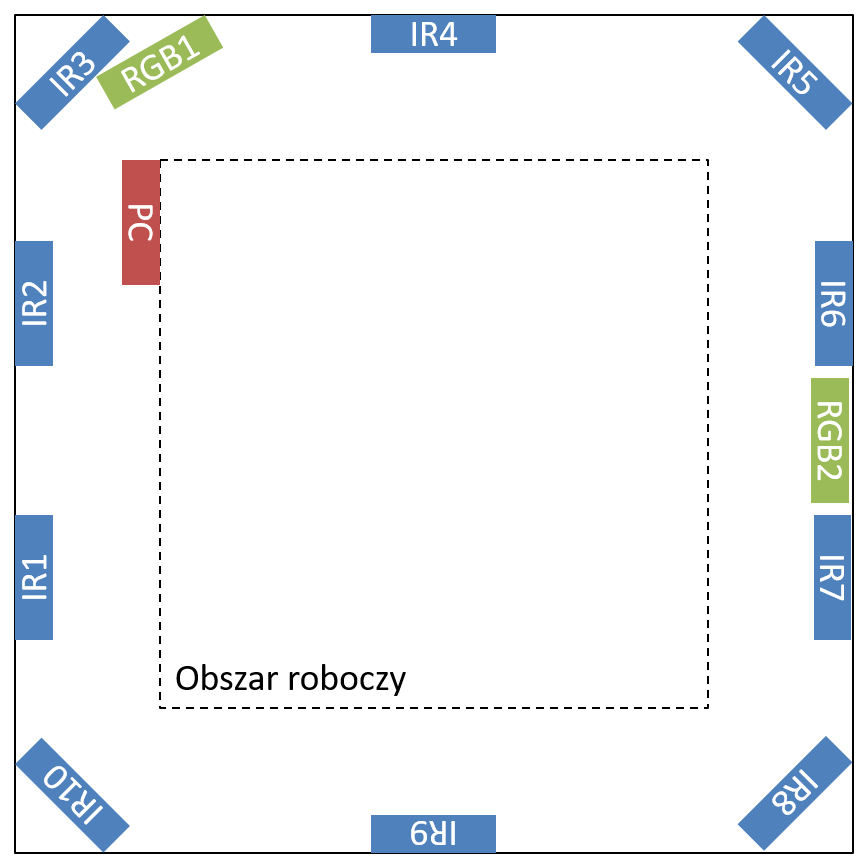
\includegraphics[width=0.75\textwidth]{images/viconSetup.png}
	\caption{Rysunek przedstawiający konfigurację sprzętową systemu Vicon dostępnego na Politechnice Łódzkiej.}
	\label{fig:literature:vicon:lutSetup}
\end{figure}

Kamery wykorzystane w~systemie Vicon posiadają filtr przepuszczający jedynie fale z~zakresu światła podczerwonego, co pozwala na stosunkowo łatwe wyodrębnienie z~rejestrowanego obrazu markerów odbijających światło podczerwone. Markery są elementami pokrytymi farbą odbijającą padające na nie światło w~kierunku źródła emisji promieni. Ponieważ w~przypadku zastosowanych kamer źródło światła jest umieszczone tuż obok obiektywu, oświetlone markery stanowią najjaśniejsze punkty na rejestrowanym obrazie. Na rysunku \ref{fig:literature:qualisys:markers} zaprezentowany został przykładowy zestaw markerów wykorzystywanych w~omawianym systemie śledzenia ruchu, natomiast na rysunku \ref{fig:literature:vicon:markers} widać aktora w~kombinezonie, przy którym owe markery są przymocowane. Markery wykorzystywane są do oznaczenia części ciała człowieka, których ruch będzie śledzony.

\begin{figure}[!htp]
	\centering	
	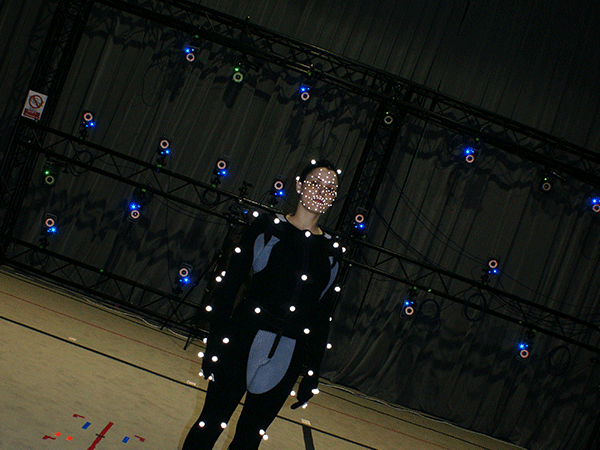
\includegraphics[width=0.75\textwidth]{images/markers-suits-600x450.png}
	\caption{Zestaw znaczników pasywnych w~systemie Vicon umieszczonych na ciele aktora w~trakcie sesji śledzenia ruchu \cite{ViconMarkersSet}}
	\label{fig:literature:vicon:markers}
\end{figure}

\begin{figure}[!htp]
	\centering	
	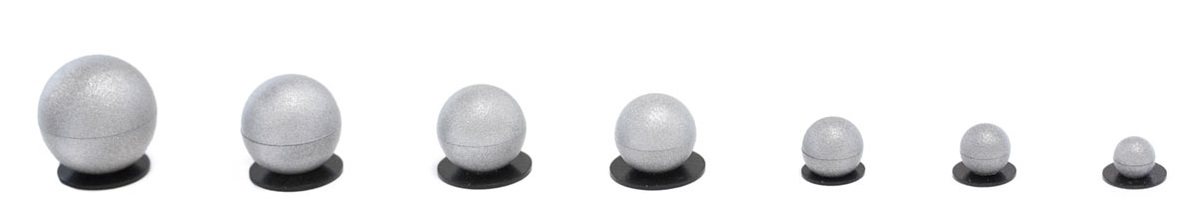
\includegraphics[width=0.75\textwidth]{images/super-spherical-markers-hero.jpg}
	\caption{Pasywne markery wykorzystywane w~optycznych systemach śledzenia ruchu\cite{QulisysMarkers}}		
	\label{fig:literature:qualisys:markers}
\end{figure}

Oprócz kamer i~markerów, istotnym elementem optycznego systemu śledzenia ruchu jest oprogramowanie obsługujące system. Jest ono odpowiedzialne za synchroniczną analizę sekwencji obrazów zarejestrowanych przez kamery tak, aby możliwe było określenie położenia każdego z~markerów w~przestrzeni trójwymiarowej układu odniesienia. W~przypadku systemu Vicon, dostępnego na Politechnice Łódzkiej, rekonstrukcja przestrzeni trójwymiarowej odbywa się na podstawie sekwencji obrazów z~maksymalnie 10 kamer. Aby możliwe było wyznaczenie położenia markera w~przestrzeni trójwymiarowej musi być on \textsl{widziany} przez minimum 3 kamery w~tym samym czasie. Pozwala to na precyzyjne wyznaczenie jego wszystkich współrzędnych za pomocą triangulacji. Jednakże zbudowanie profesjonalnego systemu śledzenia ruchu złożonego jedynie z~3 kamer byłoby niewystarczające ze względu na możliwość przysłonięcia markerów przez części ciała w~trakcie wykonywania ruchu. Zwiększenie liczby kamer pozwala na obserwowanie sceny przez większą ich liczbę, co zwiększa prawdopodobieństwo, że w~trakcie nawet złożonych ruchów przynajmniej 3 kamery zarejestrują każdy z~markerów. Dodatkowo redundancja danych, dla lepiej widocznych markerów, sprzyja zwiększeniu dokładności wyznaczania ich pozycji. Oczywiście może się zdarzyć, że pomimo zastosowania wielu kamer marker zostanie zauważony przez mniej niż 3 kamery. W~takiej sytuacji rolą oprogramowania jest oszacowanie przybliżonego położenia danego markera, przykładowo na podstawie jego relacji do położenia innych markerów i~ich trajektorii ruchu.\\

Kolejnym ważnym elementem, za który odpowiada oprogramowanie systemu śledzenia ruchu jest etykietowanie (\emph{ang. labelling}) śledzonych markerów. Dzięki temu możliwe jest określenie wzajemnych relacji pomiędzy poszczególnymi markerami i~nadanie im dodatkowego znaczenia poza wyznaczeniem położenia w~przestrzeni np.: powiązania pomiędzy markerami, przypisanie kilku markerów do jednego obiektu na scenie itp. Proces ten, po wcześniejszym zdefiniowaniu wzajemnych relacji pomiędzy markerami, jest zazwyczaj automatyzowany i~wymaga korekty ze strony operatora systemu jedynie w~sytuacjach kiedy nie jest możliwa pełna rekonstrukcja sceny, np. gdy zbyt wiele markerów jest niewidocznych dla kamer i~oprogramowanie nie jest w~stanie oszacować ich położenia, a~co za tym idzie niemożliwe jest prawidłowe przypisanie zbioru etykiet.\\ 

Rozpatrując śledzenie ruchu człowieka, istotne jest aby oprogramowanie było w~stanie kompensować różnicę między ruchem markerów jaki został zarejestrowany, a~ruchem postaci jaki został faktycznie wykonany. Szczególnie jest to widoczne w~przypadku obrotów kończyn wokół własnej osi. Aby jak najlepiej odzwierciedlić taki ruch, markery powinny być umieszczone bezpośrednio na ciele w~miejscach nie wrażliwych na przesunięcia względem układu kostnego człowieka - w~pobliżu kości, w~miejscach pozbawionych tkanki mięśniowej. Jednak i~to nie gwarantuje, że markery umieszczone na powierzchni ciała wykonają taki sam ruch jak kończyna. Badania mające na celu określenie różnicy pomiędzy ruchem jaki wykonywany jest przez kość lub staw, a~tym jak jest on widoczny na podstawie markerów umieszczonych na powierzchni skóry prowadzone były już w~latach 90-tych XX wieku \cite{Sati2016,Reinschmidt2016,Holden2016}. Reinschmidt i in. \cite{Reinschmidt2016} na przykładzie badania zgięcia kolana wykazał, że średnia różnica pomiędzy faktycznym ruchem kości, a~ruchem zarejestrowanym przez markery może wynosić od $4.1\degree$ do $5.3\degree$ w~zależności od osi, w~której ruch ten się odbywał. Sati i in. \cite{Sati2016} oraz Holden i in. \cite{Holden2016} uzyskali zbliżone rezultaty dodatkowo zauważając, że markery mogą ulec przesunięciu w~trakcie wykonywania ruchu nawet o~$2cm$ \cite{Sati2016}, co również może wypaczyć uzyskane wyniki.\\ 

Optyczne systemy śledzenia ruchu z~aktywnymi markerami działają i~są zbudowane w~analogiczny sposób do systemów z~markerami pasywnymi. Podstawową różnicą pomiędzy tymi dwoma systemami śledzenia ruchu jest to, że aktywne markery są źródłem światła co eliminuje konieczność wyposażenia całego systemu w~dodatkowe urządzenia do oświetlania sceny. Przykładem realizacji takiego systemu może być wielokamerowy system Impulse X2 firmy PhaseSpace \cite{PhaseSpaceWebsite}.\\

Niewątpliwą zaletą optycznych systemów śledzenia z~markerami jest ich wysoka dokładność szacowania pozycji śledzonych markerów przy jednoczesnej swobodzie wykonywania ruchów. Oficjalna specyfikacja systemu Vicon, a~także niezależne badania wykorzystujące ten system, pokazują że jest on w~stanie oszacować położenie markerów z~dokładnością $\pm0.5mm$, a~ich obrót z~dokładnością $\pm0.5 \degree$ \cite{ViconSpec, Windolf2008}. Dzięki tej precyzji wykorzystywane są one zarówno w~przemyśle rozrywkowym np. przy tworzeniu animacji postaci na potrzeby gier i~filmów, jak i~w~analizie ruchu na potrzeby sportu, czy medycyny \cite{Perry2012, Even-zohar1984}. 

Większość oferowanych obecnie komercyjnych optycznych systemów śledzenia ruchu pracuje standardowo z~częstotliwością 100 Hz -- 160 Hz, jednak możliwe jest także używanie ich w~trybie 500Hz i~więcej. Zwiększenie częstotliwości pomiarów wiąże się zazwyczaj z~obniżeniem ich dokładności.
Główną wadą omawianych systemów jest ich cena, która sprawia, że są one praktycznie niedostępne dla użytkowników chcących zbudować taki system śledzenia ruchu w~warunkach domowych. Wystarczy wspomnieć, że koszt zakupu systemu śledzenia ruchu firmy Vicon złożonego z~10 kamer z~filtrem podczerwonym na potrzeby Centrum Technologii Informacyjnych Politechniki Łódzkiej  wyniósł w~2014 roku ok. 1000 000 zł.
 
\subsubsection*{Optyczne systemy śledzenia ruchu nie wymagające markerów}\label{chap:mocaps:Kinect}
Drugim rodzajem optycznego systemu śledzenia ruchu są systemy niewymagające zastosowania markerów. Bezmarkerowe systemy także możemy podzielić na systemy aktywne i~pasywne \cite{Mundermann2006}. Aktywne systemy stosują emisję światła (najczęściej ustrukturyzowanego), widzialnego bądź podczerwonego, oświetlającego śledzone obiekty, natomiast pasywne rejestrują jedynie obrazy z~kamer wideo i~rozpoznają ruch na podstawie analizy zawartości obrazów. \\
Systemy aktywne wykorzystują zróżnicowane techniki emisji światła do określenia odległości pomiędzy urządzeniem pomiarowym danego systemu a~obserwowanym obiektem. Przykładową techniką jest oświetlenie sceny ustrukturyzowaną mapą punktów świetlnych, której odkształcenie pozwala określić, w~jakiej odległości przed kamerą znajdują się dany obiekty. Technika ta jest wykorzystywana między innymi przez kontroler Microsoft Kinect v1 \cite{flatley2011}, czy kamerę 3D systemu Intel RealSense \cite{intelRealSenseWebsite}. Inną popularną techniką określania odległości w~jakiej znajduje się obserwowany obiekt, wykorzystywaną przykładowo w~kontrolerze Microsoft Kinect v2 \cite{kinect2Spec}, jest czas dotarcia wiązki światła do tego obiektu (ang. \emph{Time-of-Flight}) \cite{Hansard2013}.

Zarówno w~systemach aktywnych jak i~pasywnych kluczowym etapem przetwarzania danych jest wyodrębnienie pierwszego planu i~oddzielenie go od tła. Metody wykorzystywane na tym etapie są często opisywane w~literaturze \cite{wang2003recent}\cite{rosenhahn2008markerless}\cite{guan2009estimating}\cite{surer2011markerless}\cite{corazza2006markerless}. Po separacji pierwszego planu od tła, zawierającego obraz postaci, kolejnym etapem jest znalezienie najbliższej obrazowi postaci, konfiguracji modelu człowieka, który jest jego reprezentacją w~systemie komputerowym.\\ 

Optycznym, bezmarkerowym i~zarazem aktywnym systemem śledzenia ruchu, który niewątpliwie odniósł największy sukces komercyjny i~posiada największą rozpoznawalność jest system wbudowany w~kontroler Microsoft Kinect. Obecnie dostępne są dwie wersje tego kontrolera, które znacząco różnią się sposobem działania. Starsze z~urządzeń, Microsoft Kinect v1, swoje działanie opiera na ustrukturyzowanej mapie oświetlenia podczerwonego, natomiast Microsoft Kinect v2 mierzy czas dotarcia wiązki światła od kontrolera do śledzonej postaci. W~dalszej części niniejszej pracy (rozdział \ref{chap:characteristics}) szczegółowo zostało opisane działanie kontrolera Microsoft Kinect v1 z~uwagi na fakt, że opracowana autorska metoda śledzenia ruchu wykorzystuje to właśnie urządzenie. 

Systemy śledzenia ruchu, zaimplementowane w~każdej z~dwóch wersji kontrolera Microsoft Kinect, zostały domyślnie zaprojektowane do śledzenia ruchów wykonywanych przez człowieka. Wykorzystywanie ich przykładowo do śledzenia ruchu zwierząt lub przedmiotów wymaga ingerencji w~proces przetwarzania sygnałów realizowany przez wspomniane kontrolery \cite{Nirjon2012}.

System śledzenia ruchu człowieka, zaimplementowany w~kontrolerze Microsoft Kinect, w~takiej konfiguracji w~jakiej dostarcza go producent, jest systemem do zastosowań rozrywkowych dla użytkownika domowego. Istnieją jednak bezmarkerowe systemy śledzenia ruchu człowieka adresowane do zastosowań profesjonalnych. Jako przykład może posłużyć system Organic Motion zaprezentowany na konferencji SIGGRAPH w~2012 roku. Jest to system wielokamerowy (8--18 urządzeń), który rekonstruuje zmienność obiektu 3D w~czasie na podstawie triangulacji wspólnych punktów rozpoznanych na zsynchronizowanych obrazach 2D \cite{Brooks2012}.

W swoim artykule Brooks i~Czarowicz \cite{Brooks2012} porównują podstawowe cechy systemów Organic Motion oraz systemu wbudowanego w~kontroler Microsoft Kinect v1. W~tabeli \ref{tab:literature:markerless:comparison} znajduje się skrócone porównanie tych dwóch systemów. 

\begin{table}[!htp]
	\caption{Porównanie cech charakterystycznych systemu Organic Motion oraz systemu wbudowanego w~kontroler Microsoft Kinect v1}
	\label{tab:literature:markerless:comparison}
	\footnotesize
	\noindent
	\centering
	\begin{tabular}{|l|c|c|}
															
		\hline 
		                                 & \textbf{Kinect} & \textbf{Organic Motion} \\ 
		\hline 
		\textbf{Częstotliwość}        & 30Hz            & 30Hz -- 120Hz           \\ 
		\hline 
		\textbf{Wymiarowanie kości szkieletu} & \begin{tabular}{@{}c@{}}Szacowanie \\ Zmienne w~czasie\end{tabular}
		& \begin{tabular}{@{}c@{}}Dokładny pomiar \\ Stały w~czasie\end{tabular} \\
		\hline 
		\textbf{Śledzenie stóp}        & Brak            & Jest                    \\ 
		\hline 
		\textbf{Śledzenie palców}      & Brak            & Brak                    \\ 
		\hline 
		\textbf{Śledzenie 360$\degree$} & Brak            & Jest                    \\ 
		\hline 
		\textbf{Opóźnienie}            & 250ms           & 50--100ms               \\ 
		\hline 
		\textbf{Rozdzielczość}         & 640x480px       &                         
		\begin{tabular}{@{}c@{}}8 -- 18 kamer \\ 640x480px każda\end{tabular} \\ 
		\hline 
	\end{tabular}
\end{table}

Cechy przedstawione w~powyższej tabeli pozwalają zauważyć kilka istotnych różnic pomiędzy porównywanymi systemami, które mają znaczący wpływ na działanie i~obszary możliwych zastosowań dla każdego z~nich. Warto zauważyć, że system oparty o~kontroler Microsoft Kinect v1, w~konfiguracji zalecanej przez jego producenta, opiera się o~pojedyncze urządzenie rejestrujące obraz z~rozdzielczością 640x480px co sprawia, że jesteśmy pozbawieni możliwości śledzenia małych ruchów wykonywanych na przykład przez palce, czy stopy. Są to ruchy zbyt szczegółowe by można było je skutecznie zarejestrować i~wyodrębnić na tak niskiej rozdzielczości obrazu. Dodatkowo, pojedyncze urządzenie sprawia, że ruch obserwowany jest tylko z~jednej płaszczyźnie, więc tracimy informację o~ruchu jaki wykonywany jest przykładowo za plecami użytkownika. W~przypadku systemu Organic Motion wykorzystanie większej liczby kamer daje możliwość pełnej obserwacji dookoła użytkownika w~$360\degree$. Obraz uzyskany z~wielu kamer daje sumarycznie większą rozdzielczość co pozwala na zarejestrowanie szczegółowych ruchów. Daje także możliwość dokładnego, stałego w~czasie, wymiarowania poszczególnych elementów modelu ciała człowieka (w szczególności długości jego kości) zamiast przybliżonego ich szacowania na podstawie chwilowych danych, co ma wpływ na częstą zmienność tych pomiarów. Wszystko to pokazuje, że, o~ile w~systemach rozrywkowych, gdzie nie ma konieczności uzyskiwania stabilnych i~dokładnych pomiarów oraz~śledzenia ruchu, kontroler Microsoft Kinect jest wystarczający. Natomiast aplikacje związane na przykład z~biomechaniką wymagają rozbudowanych systemów wielokamerowych.\\

Przybliżone powyżej systemy wizyjne, zarówno te wykorzystujące markery jak i~bezmarkerowe, osiągają wysoką dokładność śledzenia ruchu w~konfiguracjach wielokamerowych umieszczonych wewnątrz pomieszczenia, gdzie system nie jest podatny na działanie światła słonecznego. W~przypadku śledzenia ruchu wykonywanego w~innych warunkach niż studyjnych, przykładowo w~wodzie, systemy oparte o~inne techniki niż optyczne np. rejestrując prędkości ruchu śledzonych części ciała.

\subsection{Systemy nieoptyczne}

\subsubsection*{Systemy inercyjne i~magnetyczne}\label{chap:mocaps:IMU}
Systemy inercyjne oraz systemy magnetyczne opierają swoje działanie na pomiarach wielkości fizycznych (podać konkretnie) występujących w~trakcie wykonywania ruchu. Wykorzystują one moduły zbudowane z~czujników pozwalających na pomiar wspomnianych wielkości, jakie występują w~momencie wykonywania ruchu. Systemy inercyjne wykorzystują dwa czujniki bezwładnościowe: akcelerometr oraz żyroskop. Każdy z~nich może być jedno, dwu lub trójosiowy, co przekłada się na liczbę kierunków ruchu, w~którym może być dokonany pomiar.\\
Akcelerometry są to czujniki mierzące siłę oddziałującą liniowo wzdłuż poszczególnych osi. Pomiar oddziałującej siły wyrażany jest w~odniesieniu do siły grawitacji, co teoretycznie pozwala na określenie z~jakim przyspieszeniem w~każdej z~mierzonych osi porusza się dany czujnik. W~praktyce, precyzyjne określenie przyspieszeń w~każdej osi, a~dalej na tej podstawie określenie odległości na jaką przesunął się czujnik jest utrudnione ze względu na duże zaszumienie danych. Możliwe jest natomiast przybliżone oszacowanie kąta obrotu danego czujnika, będącego w~spoczynku, względem siły grawitacji.\\
Drugim z~czujników inercyjnych jest żyroskop, który pozwala zmierzyć prędkość kątową względem każdej z~osi z~jaką obraca się czujnik. W~przypadku pozostawania czujnika bez ruchu, pomiary dla każdej z~osi powinny wynosić~0. Podobnie jak w~przypadku akcelerometru, zaszumienie danych znacząco utrudnia precyzyjne określenie o~jaki kąt obrócił się czujnik.\\
Czujnikiem magnetycznym, jaki wykorzystywany jest w~magnetycznych systemach śledzenia ruchu, jest magnetometr. Czujnik ten pozwala na określenie jak jest on obrócony względem pola magnetycznego ziemi.\\
Czujniki te najczęściej wykorzystywane są w~konfguracji para akcelerometr--żyroskop lub trójki akcelerometr--żyroskop--magnetometr. Para akcelerometr--żyroskop występuje w~literaturze anglojęzycznej pod nazwą \emph{ang. Innertial Measurement Unit -- IMU} natomiast trójka wspomnianych czujników nazywana jest \emph{ang. Magnetic, Angular Rate, and Gravity -- MARG}.\\
Wykorzystywanie tych czujników w~parze lub trójce ma na celu połączenie ze sobą ich sygnałów i~dzięki temu zmniejszenie wpływu szumów na pomiary uzyskiwane przez każdy z~nich z~osobna. Metody łączenia ze sobą sygnałów z~czujników inercyjnych oraz magnetometru, a także identyfikacja szumów jakie na nie działają, od wielu lat są przedmiotem badań uczonych ze wszystkich ośrodków badawczych zajmujących się śledzeniem i~analizą ruchu i~są wciąż kontynuowane. Jako przykłady prac związanych z~tym zagadnieniem można przytoczyć chociażby propozycję wykorzystania transformaty Fouriera do badania szumu magnetometrów w~zakresie niskich częstotliwości $(0Hz, 5Hz]$. Badania te były prowadzone przez zespół włoskich naukowców pod przewodnictwem Maurizio Candidiego już w~latach 70-tych XX wieku \cite{Candidi1974} na potrzeby przemysłu kosmicznego. W~latach 90-tych zaszumienie danych z czujników inercyjnych: akcelerometru i~żyroskopu oraz metod kompensacji tych szumów było obiektem badań przedstawionych przez S. Woolvena i~D. B. Reida z~Uniwersytetu w~Ontario \cite{Woolven1994}. Autorzy w swoim artykule zaproponowali łączenie danych z~dwóch wspomnianych czujników inercyjnych za pomocą filtru Kalmana jako jednej z~metod kompensacji ich szumów. Wśród współczesnych badań znaleźć można propozycję zastosowania falek do odszumiania pomiarów czujników inercyjnych (ElSheimy  \cite{ElSheimy2004}). Zastosowanie ich w~kontekście systemu nawigacji inercyjnej (INS) pozwoliło zmniejszyć niemal dziesięciokrotnie wariancję wyznaczonego kierunku poruszania się nawigowanego obiektu oraz trzykrotnie przyspieszyć ustabilizowanie się estymacji obranego kierunku ruchu. W~dotychczas dyskutowanych publikacjach, metodą łączenia danych z~wykorzystywanych czujników był filtr Kalmana. Jego główną wadą jest jednak wysoka złożoność obliczeniowa spowodowana wykorzystaniem rachunku macierzowego. W~2015 roku Pasquale Daponte wraz ze swoim zespołem przedstawili publikację badającą, alternatywną do filtru Kalmana, metodę łączenia danych z~czujników inercyjnych i~magnetycznych \cite{Daponte2015}. Obiektem ich badań była metoda zmniejszającego się gradientu wykorzystywana wcześniej przez Roberta Mahony'ego \cite{Mahony2005a} oraz Sebastiana Madgwicka \cite{Madgwick2011}. Autorzy dyskutowanego artykułu wskazali trzy główne zalety badanej przez nich metody w porównaniu do wykorzystywanego powszechnie filtru Kalmana: mniejsza złożoność obliczeniowa, szybsza stabilizacja uzyskiwanych wyników i~ich lepsza stabilność w~czasie. Dodatkowo zwrócili uwagę na wykorzystanie kwarternionów przez badany przez nich algorytm zamiast kątów Eulera, co z~kolei ma wpływ na możliwość szerszego wykorzystania otrzymanych wyników w~dalszych obliczeniach oraz uniknięcia niejednoznaczności obrotów. \\
Warto zauważyć, że zarówno moduł zbudowany z~pary czujników inercyjnych jak i~moduł zawierający akcelerometr, żyroskop oraz magnetometr określają jak względem poszczególnych osi obrócony jest dany moduł. W~przypadku wykorzystania tylko czujników inercyjnych, możliwe jest określenie obrotu wokół dwóch osi prostopadłych do osi wyznaczonej przez siłę grawitacji. Na rysunku \ref{fig:literature:imu:coordination} są to osie X i~Y. W~przypadku wykorzystania również magnetometru możliwe jest określenie obrotów wokół każdej z~tych osi. Warto również zauważyć, że układ współrzędnych połączonych czujników, w~jakim przedstawione są obroty wokół każdej z~osi, odpowiada osiom w~układzie współrzędnych Ziemi. Oznacza to, że w~przypadku wykorzystania wszystkich trzech czujników, możliwe jest określenie orientacji modułu względem czterech stron świata (obrót wokół osi Z) oraz względem płaszczyzny Ziemi (obroty względem osi X i~Y).

\begin{figure}[!htp]
	\centering	
	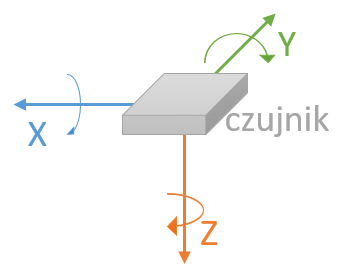
\includegraphics[width=0.75\textwidth]{images/IMUAxes.png}
	\caption{Układ współrzędnych dla czujników inercyjnych i~magnetycznych.}
	\label{fig:literature:imu:coordination}
\end{figure}

Nie ma natomiast możliwości precyzyjnego określenia położenia modułu w~przestrzeni na podstawie jedynie akcelerometru, żyroskopu i~magnetometru na podstawie przemieszczenia wyznaczonego metodami zliczeniowymi. Spowodowane jest to znaczącymi szumami występującymi w~pomiarach, a~przez to niską dokładnością uzyskiwanych wyników. Fakt ten ma wpływ na sposób budowania systemów śledzenia opartych na takich urządzeniach. W~przypadku śledzenia ruchu człowieka wymagane jest uzupełnienie pomiarów poprzez zdefiniowanie hierarchicznego modelu szkieletu ludzkiego, zawierającego informację o~długościach poszczególnych kości. Umożliwia to oszacowanie położenia poszczególnych stawów na podstawie orientacji czujników umieszczonych na poszczególnych częściach ciała. W~związku z~tym, duży wpływ na dokładność śledzenia ruchu w~systemach wykorzystujących czujniki inercyjne i~magnetyczne ma dokładność pomiaru długości poszczególnych kości.\\
Przykładem komercyjnej implementacji takiego systemu może być rozwiązanie zaproponowane przez firmę Xsens, które z~powodzeniem wykorzystywane jest zarówno do śledzenia ruchu na potrzeby animacji \cite{XsensEnt}, jak i~do analizy ruchu u sportowców \cite{XsensSport1,XsensSport2}, czy w~procesie rehabilitacji motorycznej \cite{XsensRehab}. Dinu i in. w~swojej pracy \cite{Dinu2016} porównał dokładność systemu Xsens z~systemem Vicon w~kilku przypadkach użycia. Pierwszym z~nich było porównanie pozycji stawów oszacowanych za pomocą systemów Xsens i~Vicon dla znanej obu systemom pozy związanej z~procesem kalibracji. Przyjmując pomiary Vicona jako referencyjne, autorzy wyznaczyli średniokwadratowy błąd szacowania położenia stawów przez system XSens na wartość poniżej $0.5mm$. Należy jednak pamiętać, że oba systemy "wiedziały"' jak będą wyglądały pozy w~jakich będzie stał użytkownik. W~przypadku śledzenia dowolnego ruchu błąd oszacowania występujący między systemami śledzenia XSens i~Vicon wzrósł w~zależności od osi do niemal $5.5mm$,

Widzimy więc, że systemy śledzenia ruchu oparte o~czujniki inercyjne i~magnetyczne, przy wykorzystaniu odpowiedniej jakości urządzeń pomiarowych i~dokładnym modelu kości są w~stanie dość precyzyjnie śledzić ruch postaci i~pozycjonować jej stawy w~przestrzeni. Jednak na przykładzie zastosowań sportowych \cite{XsensSport1,XsensSport2} należy zauważyć, że układy IMU i~MARG nie są wystarczające do oszacowania położenia śledzonej postaci na scenie, a~jedynie do odtworzenia jej pozy. Aby śledzić przemieszczenie się całej postaci wykorzystywany jest dodatkowy system umożliwiający lokalizowanie obiektów w~przestrzeni. W~zależności od powierzchni na jakiej odbywa się ruch może być to system GPS, czy systemy oparte o~technologię LPM (\emph{ang. local position measurement}). GPS przeznaczony jest do lokalizowania postaci na bardzo dużej powierzchni w~warunkach zewnętrznych, przy dokładności określenia położenia rzędu kilku metrów\footnote{Według danych zamieszczonych na \url{http://www.gps.gov/} dokładność systemu GPS może wynieść do $3.5m$.}. Technologie LPM pozwalają na użycie ich zarówno wewnątrz budynków, jak i~na zewnątrz, wymagają jednak dodatkowych urządzeń obserwujących określony obszar, na którym odbywa się ruch. Jako przykład realizacji systemu LPM może posłużyć system firmy Inmotio\cite{inmotio} wykorzysujący technologię radiową RFID (identyfikacja radiowa, \emph{ang. Radio-frequency identification}), która pozwala określić położenie śledzonej postaci na podstawie triangulacji oraz pomiaru mocy sygnału pomiędzy stacjami bazowymi a~odbiornikiem. Przykładowa konfiguracja takiego systemu widoczna jest na rysunku \ref{fig:literature:inmotio:setup}). Szczegółowy opis działania systemu Xsens można znaleźć w~pracy Roetenberg i in. \cite{Roetenberg2009}.

\begin{figure}[!htp]
	\centering	
	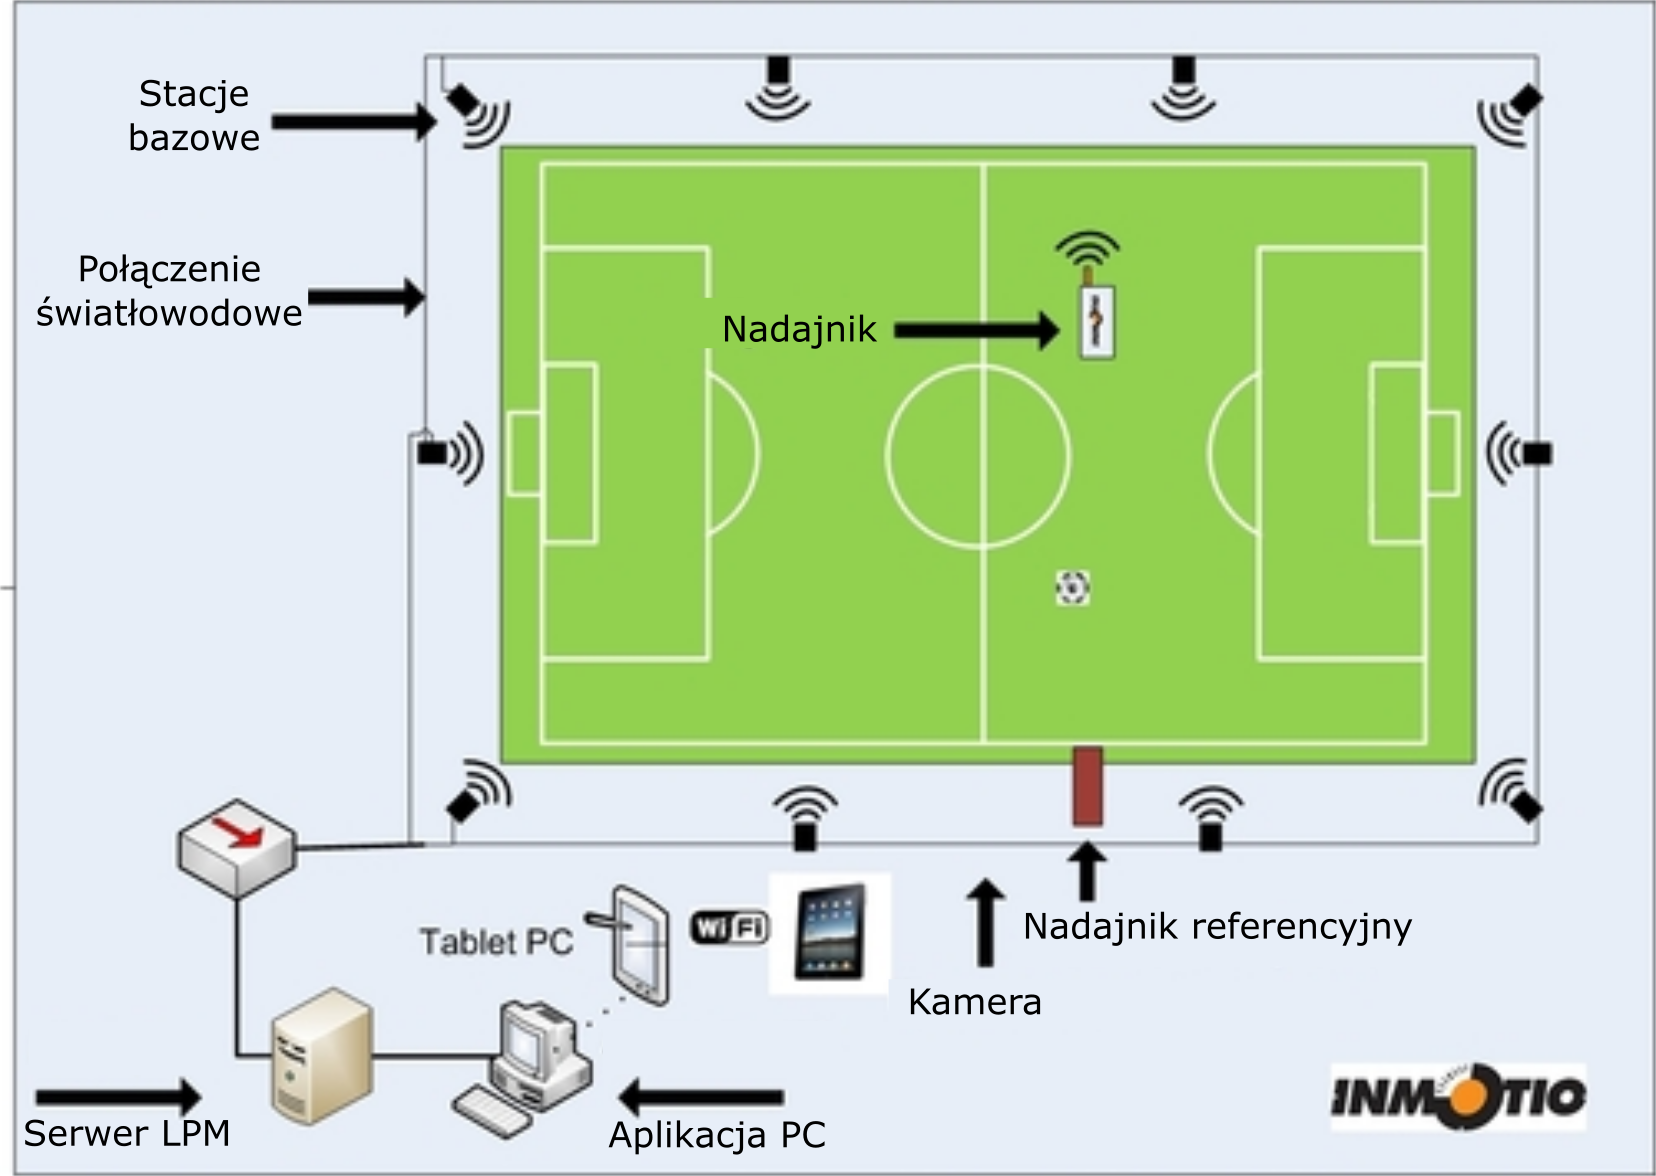
\includegraphics[width=0.75\textwidth]{images/lpm.png}
	\caption{Przykładowa konfiguracja systemu LPM firmy Inmotio\cite{inmotio}}	
	\label{fig:literature:inmotio:setup}	
\end{figure}

Systemy śledzenia ruchu oparte o~czujniki inercyjne i~magnetycze są także obiektem prac badawczych mających na celu poprawę dokładności śledzenia ruchu. Zhou i~Hu \cite{Zhou2005,Zhou2006} zaproponowali, na podstawie badań opartych o śledzenia ruchu stawów ręki, wykorzystanie algorytmu symulowanego wyżarzania w~celu zmniejszenia błędów pomiarowych czujników oraz zastosowali rozszerzony filtr Kalmana do połączenia sygnałów z~sensorów. Na potrzeby badania swojej metody, Zhou i~Hu wykorzystali komercyjny, inercyjny system śledzenia ruchu firmy Xsens, natomiast dane referencyjne uzyskali za pomocą wizyjnego systemu śledzenia ruchu firmy Vicon. Zaproponowana przez nich metoda pozwoliła na poprawienie dokładności śledzenia ruchu stawów ręki o~$26\%$ z~około $2.3 cm$ do $1.7 cm$.\\

W przypadku systemów śledzenia ruchu człowieka opartych o~IMU i~MARG wpływ na dokładność wyznaczenia położenia poszczególnych stawów ma umiejscowienie czujników na ciele. Badania na ten temat prowadzili m.in. Vanegas i~Stirling \cite{Vanegas2015}. Badania te wykazały, że optymalnym miejscem umieszczenia tego typu sensorów są okolice środka masy danej części ciała lub obiektu. W~przypadku umieszczenia czujników na ciele człowieka pomocne okazują się być wyniki badań prowadzonych w~połowie lat 90-tych przez Paolo de Leva z~Uniwersytetu stanu Indiana. De Leva w~swojej pracy, dotyczącej badań nad środkami mas poszczególnych części ciała\cite{DeLeva1996}, rozwinął wcześniejsze badania Zatsiorskiego i~Seluyanova \cite{549} i~wyznaczył położenie poszczególnych środków mas. Rysunek \ref{fig:centerOfMass} przedstawia diagram rozmieszczenia środków mas dla każdej z~części ciała według badań de Leva.

\begin{figure}[!htp]
	\centering	
	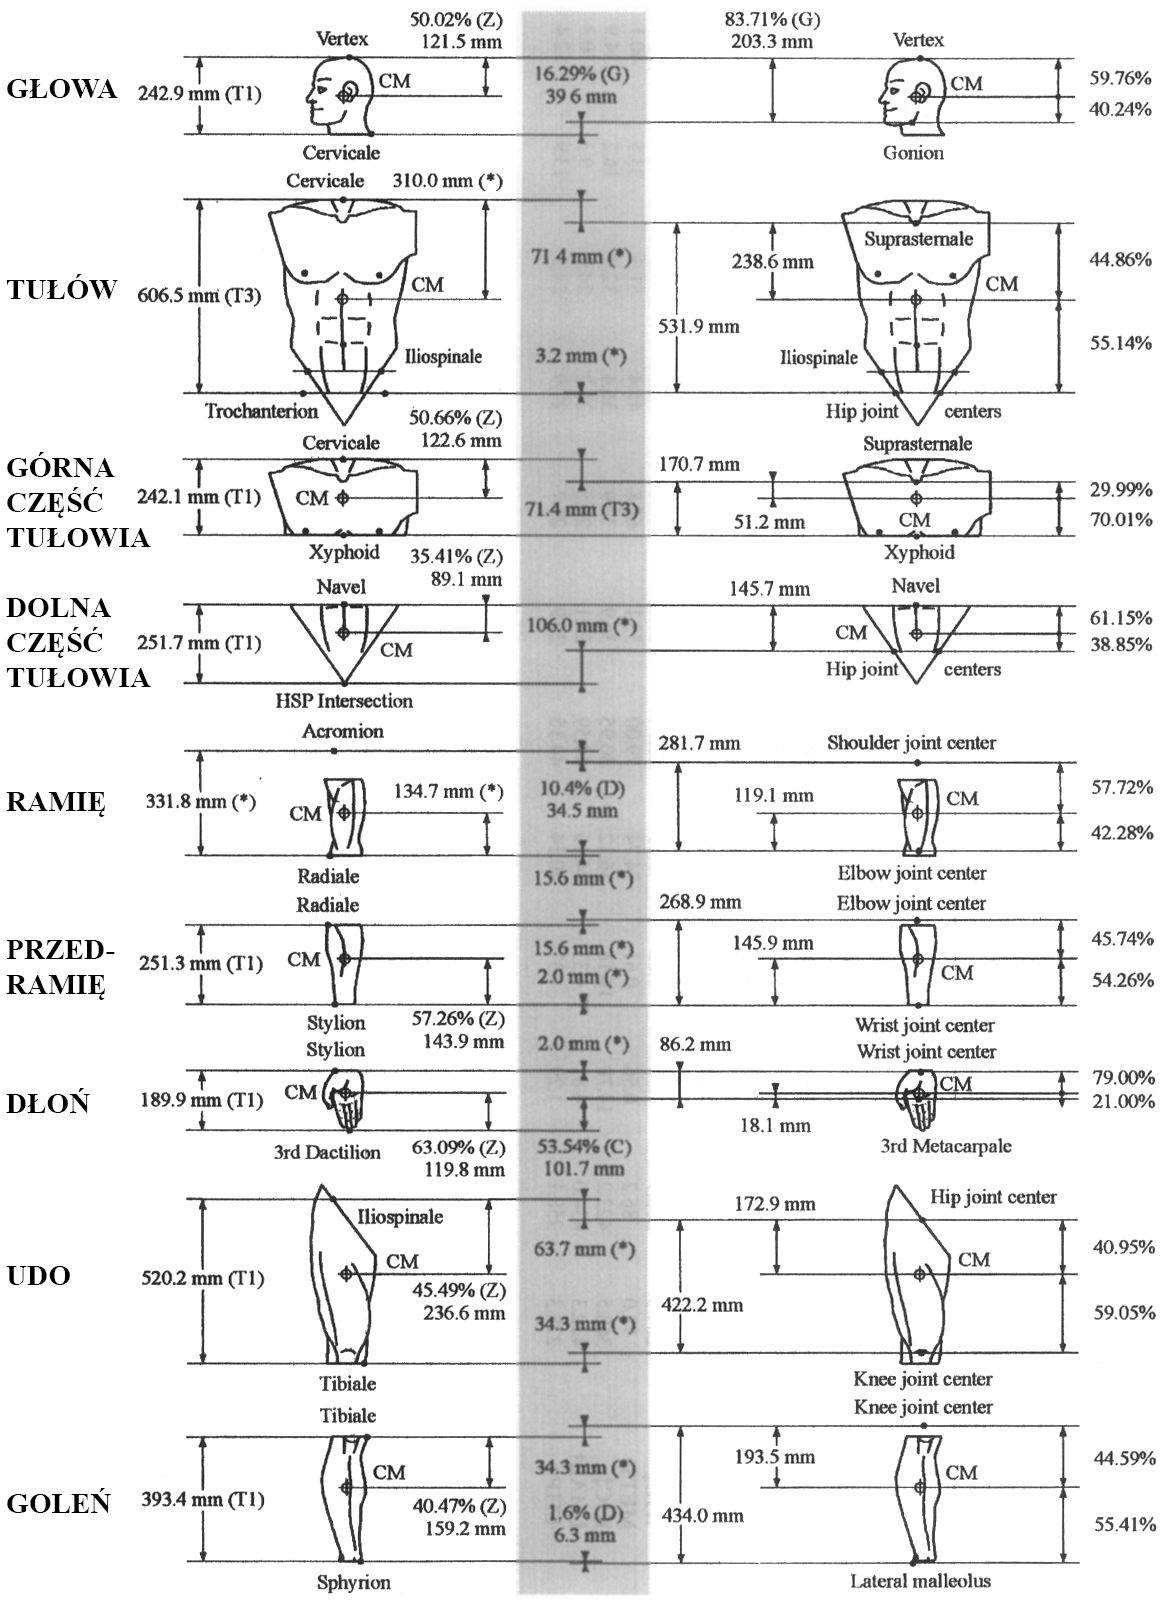
\includegraphics[width=0.75\textwidth]{images/centerOfMass.png}
	\caption{Rozmieszczenie środków mas poszczególnych części ciała człowieka według propozycji de Leva\cite{DeLeva1996}}	
	\label{fig:centerOfMass}	
\end{figure}

\subsubsection*{Systemy elektromagnetyczne (radiowe)}
Elektromagnetyczne systemy śledzenia ruchu opierają się o~pomiar strumienia elektromagentycznego wytworzonego między nadajnikiem umieszczonym na ciele postaci, której ruch jest śledzony, a~odbiornikami, które otaczają obszar, na którym odbywa się śledzenie ruchu. Zarówno nadajnik jak i~odbiorniki zbudowane są z~kilku prostopadłych cewek, co pozwala na śledzenie ruchu w~6 stopniach swobody (położenie oraz obroty). Dokładne położenie nadajnika w~przestrzeni wyznaczone jest za pomocą triangulacji uzyskiwanych pomiarów. Elektromagnetyczne systemy śledzenia ruchu są podatne na zakłócenia wynikające z~obecności elementów metalowych lub magnetycznych w~pobliżu obszaru, na którym odbywa się śledzenie. W~szczególności źródłem  takiego zakłócenia mogą być stalowe elementy konstrukcyjne budynku gdzie znajduje się system śledzenia (np. pręty zbrojeniowe w~stropie czy ścianach). 

\subsubsection*{Systemy akustyczne}
Akustyczne systemy śledzenia opierają się na pomiarze czasu przemieszczania się fali dźwiękowej między nadajnikami umieszczonymi na ciele osoby, której ruch był śledzony, a~odbiornikami umieszczonymi wokół obszaru, na którym ruch się odbywał. Systemy te również określają położenie nadajników na podstawie triangulacji. Niestety, są one podatne na wiele czynników naturalnych, które mogą wpływać na dokładność uzyskanych wyników. Do takich czynników należą między innymi temperatura powietrza, wilgotność, czy ciśnienie atmosferyczne. Wymienione czynniki zewnętrzne powodują zmianę szybkości przemieszczania się fali dźwiękowej i w konsekwencji, zaburzenia rozchodzenia się dźwięku. Akustyczne systemy śledzenia ruchu zazwyczaj wykorzystują ultradźwięki, więc są niesłyszalne dla człowieka.

\subsubsection*{Systemy mechaniczne}
Mechaniczne systemy śledzenia ruchu różnią się znacznie od poprzednio opisanych systemów choćby ze względu na ich ingerencję w~swobodę ruchu jaki może wykonać śledzona osoba. Podstawowym urządzeniem wykorzystywnym w~mechanicznych systemach śledzenia ruchu, jest strój nazywany egzoszkieletem, zbudowany z~szeregu czujników mechanicznych i~elektromechanicznych, np. potencjometrów, których zadaniem jest odzwierciedlenie pozy jaką przyjmuje śledzona osoba. Przykładem egzoszkieletu może być układ mechaniczny będący elementem systemu śledzenia ruchu Gypsy \cite{gypsy}. Egzoszkielet został~zaprezentowany na rysunku \ref{fig:literature:gypsy:full}.

\begin{figure}[!htp]
	\centering	
	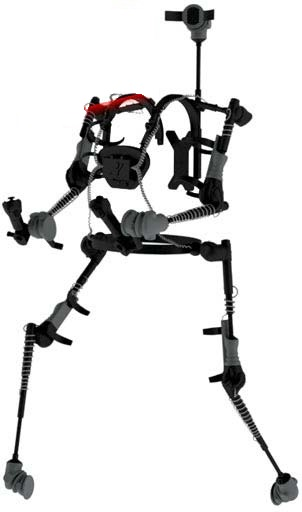
\includegraphics[height=6cm]{images/gypsy7_full.jpg}
	\caption{Egzoszkielet dla systemu MoCap Gypsy}	
	\label{fig:literature:gypsy:full}
\end{figure}

Niewątpliwą zaletą mechanicznych systemów śledzenia ruchu jest to, że jedynym urządzeniem z~jakiego się składa taki system to wspomniany egzoszkielet. Nie jest on podatny na zakłócenia swojego działania przez elementy znajdujące się w~otoczeniu, czy przysłanianie się części ciała w~trakcie ruchu. Mechaniczne systemy śledzenia ruchu zazwyczaj są w~stanie pracować w~czasie rzeczywistym. Niestety, wadą jest, wspomniane już wcześniej, ograniczenie swobody wykonywanego ruchu, co powoduje, że nie każdy rodzaj ruchu (np. dynamiczne ćwiczenia gimnastyczne) może być śledzony za pomocą układów mechanicznych .

\section{Trójwymiarowy model postaci ludzkiej} \label{chap:bodyRep}
Systemy śledzenia ruchu kończyn człowieka opierają się często na komputerowym modelu postaci, który opisuje właściwości kinematyczne modelu szkieletu oraz, jeśli to możliwe, również kształt ciała śledzonej postaci. Reprezentacja geometryczna opisująca zewnętrzny wygląd postaci jest zmapowana na jego układ szkieletowy, dzięki czemu zmiany szkieletu mogą być automatycznie przekładane na zewnętrzną pozę postaci, natomiast na podstawie kształtu i~ustawienia ciała człowieka można wnioskować jaka jest konfiguracja szkieletu. 
Nie istnieje jeden standardowy model postaci, gdyż w~zależności od zastosowań przyjmowane sa różne uproszczenia. O ile szkielet kostny dorosłego człowieka składa się z~206 kości \cite{Lasinski1990}, o~tyle w~modelach komputerowych, na potrzeby rejestracji ruchu, stosuje się ich zazwyczaj kilkadziesiąt. Przykładowo, model szkieletowy zastosowany w~kontrolerze Kinect składa się z~20 stawów i~19 kości\cite{msdn:kinectSkeleton}, zaś model szkieletowy systemu Optitrack zbudowany jest również z~20 stawów, ale połączonych ze sobą za pomocą 25 kości\cite{optitrackSkeleton} (zwiększona liczba kości w~obrębie klatki piersiowej oraz stóp). Zatem przyjęcie właściwego modelu reprezentacji postaci wpływa na swobodę ruchów (liczba stopni swobody) modelowanego układu kostnego, co z kolei przekłada się na skuteczność i~dokładność śledzenia kończyn człowieka.

\subsection{Model kinematyczny szkieletu postaci}
Model kinematyczny szkieletu postaci opisany jest za pomocą struktury przedstawiającej relacje między poszczególnymi stawami połączonymi ze sobą segmentami reprezentującymi kości. Każdy ze stawów opisany jest przez tzw. stopnie swobody definiujące w~jaki sposób segmenty (kości) połączone danym stawem mogą się wzajemnie poruszać. Teoretycznie maksymalna liczba stopni swobody danego stawu może wynosić 6, co oznacza, że staw może przesunąć się wzdłuż każdej z~3 osi $X, Y$ i~$Z$ układu współrzędnych oraz obracać się wokół każdej z~nich, jednak w~praktyce zakres ruchomości stawów człowieka jest ograniczony i~osobniczo różny. W~związku z~tym pozycja każdego ze stawów jest determinowana stopniem swobody jego rodzica. Zatem wiedząc, że staw łokciowy ma jeden stopień swobody, ruch kości przedramienia jest ograniczony tylko do jednej płaszczyzny, a~względna możliwa pozycja stawu nadgarstkowego znajduje się na łuku o~promieniu równym długości kości przedramienia.\\
%[FIxed]tutaj trzeba doprecyzować gdzie jest układ i~jaki to układ? Czy kości się przemiszczają względem siębie czy może staw ma stopień swobody.

Model kinematyczny jest zazwyczaj definiowany jako hierarchiczny układ stawów co oznacza, że wielkości opisujące dany staw są wielkościami względnymi w~odniesieniu do stawu bezpośrednio go poprzedzającego (nadrzędnego) w~hierarchii. Aby wyznaczyć wartości absolutne danego stawu, niezbędne jest przyrostowe złożenie informacji ze wszystkich stawów w~łańcuchu kinematycznym, począwszy od stawu głównego (korzenia). Korzeniem nazywamy jeden wyszczególniony staw modelu hierarchicznego, do którego doczepione są łańcuchy kinematyczne wszystkich pozostałych stawów. Korzeń może, ale nie musi mieć swojego odpowiednika w~stawach szkieletu ludzkiego. Jako przykład można przytoczyć propozycję uproszczonego modelu szkieletowego człowieka wraz z~przedstawieniem hierarchii poszczególnych segmentów oraz ich stopni swobody zaproponowaną przez Kwolek i in.\cite{Kwolek2014} i~przedstawioną na rys. \ref{fig:literature:skeletonModelHierarchy}. W~modelu kinematycznym, w~którym określona jest hierarchia jego stawów, układ współrzędnych, w~którym opisane są obroty i~położenie danego stawu, ma swój początek w~stawie poprzedzającym go (staw rodzica). Sprawia to, że wartości przypisane do poszczególnych stawów są wielkościami względnymi.

\begin{figure}[!htb]
	\centering
	\begin{minipage}{.2\textwidth}
		\centering
		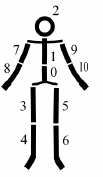
\includegraphics{images/hierarchical-structure.png}       
	\end{minipage}%
	\begin{minipage}{0.8\textwidth}
		\centering
		\scalebox{0.8}{
			\tiny
\begin{tikzpicture}[
	level 1/.style={sibling distance=5.3cm},
level 2/.style={sibling distance=2.3cm}, 
	every node/.style = {shape=rectangle, rounded corners,
    draw, align=center}]]
  \node {0. Miednica\\(\emph{ang. Pelvis})\\6 DOF}   
    child { node {3. Lewe udo\\(\emph{ang. Upper Right Leg})\\2 DOF}
    	child { node {4. Lewy piszczel\\(\emph{ang. Right Lower Leg})\\1 DOF}}
    }
    child { node {1. Kręgosłup\\(\emph{ang. Spine})\\3 DOF}    	
    	child {node{7. Prawe ramię\\(\emph{ang. Upper Right Arm})\\3 DOF}
    		child {node{8. Prawe przedramię\\(\emph{ang. Right Forearm})\\1 DOF}}
    	}
    	child {node{2. Głowa\\(\emph{ang. Head})\\3 DOF}}
	child {node{9. Lewe ramię\\(\emph{ang. Upper Left Arm})\\3 DOF}
		child {node{10. Lewe przedramię\\(\emph{ang. Left Forearm})\\1 DOF}}
	}	     
    }
    child { node {5. Prawe udo\\(\emph{ang. Upper Left Leg})\\2 DOF}
    	child { node {6. Prawy piszczel\\(\emph{ang. Left Lower Leg})\\1 DOF}}
    };
\end{tikzpicture}
		}
	\end{minipage}
	\caption{Uproszczony hierarchiczny model szkieletowy człowieka (lewo) wraz z~diagramem przedstawiającym hierarchię poszczególnych elementów(prawo)\cite{Kwolek2014}}
	\label{fig:literature:skeletonModelHierarchy}
\end{figure}

Oprócz stopni swobody pojedynczego stawu, definiuje się również stopień swobody całego modelu kinematycznego. Taka wielkość rozumiana jest jako suma stopni swobody wszystkich jego elementów. W~przypadku pełnego opisu modelu postaci możemy mieć zatem do czynienia z~modelem kinematycznym, który posiada zdefiniowanych ponad 50 stopni swobody \cite{Agarwal2006}. Nie zawsze jednak potrzebne są modele zawierające pełen opis stopni swobody. Okazuje się, że do śledzenia większości ruchów człowieka wystarczający jest model uproszczony definiujący około 30 stopni swobody \cite{Sigal2006,Kwolek2011}.\\

O ile model kinematyczny szkieletu jest w~stanie jednoznacznie opisać pozę, w~jakiej znajduje się śledzona postać w~danej chwili czasu o~tyle może okazać się to niewystarczające w~przypadku śledzenia ruchu w~środowiskach wirtualnych, w~których istotna jest interakcja postaci z~otoczeniem. W~takim przypadku niezbędne staje się określenie dodatkowo modelu kształu ciała śledzonej postaci.
		
\subsection{Model reprezentacji postaci}
Modele kształtu ciała, podobnie jak modele kinematyczne, możemy określać w~przestrzeni dwu-- lub trójwymiarowej. Zwykle wystarczające jest przybliżone odwzorowanie kształtu poszczególnych części ciała za pomocą figur geometrycznych (modele 2D) lub brył (modele 3D). Pozwala to zwizualizować budowę ciała postaci, której ruch jest śledzony, bez zbytniego obciążania procesora komputera, na którym odbywa się przetwarzanie danych pozyskanych z~systemu śledzenia. Dokładne odwzorowanie budowy ciała postaci jest możliwe dzięki wykorzystaniu popularnych przestrzennych reprezentacji geometrycznych (np.: siatka trójkątna 3D), jednak ich wykorzystanie może wpłynąć negatywnie na wydajność systemu. \\
Niezależnie jakie reprezentacje geometryczne wykorzystujemy, istotne jest takie przedstawienie kształtu ciała, aby odpowiednio zwizualizować przynajmniej śledzone ruchy. Przykładowo, jeśli wykorzystujemy trójwymiarowy uproszczony model zbudowany z~kul i~cylindrów trudne będzię zwizualizowanie niektórych obrotów ciała, przykładowo rotacji dłoni i~nadgarstka jak na rys. \ref{fig:literature:wristRotation}.\\
		
\begin{figure}[!htp]
	\centering	
	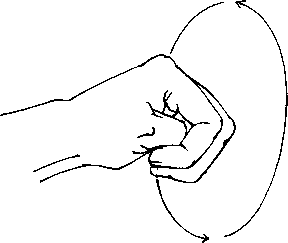
\includegraphics[height=6cm]{images/Wrist_joint_rotation.png}
	\caption{Rotacja wewnętrzna (pronacja) i~zewnętrzna (supinacja) dłoni.}	
	\label{fig:literature:wristRotation}
\end{figure}

W praktyce to w~jaki sposób aktor będzie reprezentowany w~systemie komputerowym ściśle powiązane jest z~przeznaczeniem danego systemu. Inna reprezentacja będzie konieczna dla śledzenia i~rozpoznawania pozy w~jakiej znajduje się aktor, a~inaczej jeśli śledzimy jego położenie w~przestrzeni. I~tak możemy wyróżnić następujące sposoby reprezentowania postaci:
	
\begin{itemize}
	\item \textbf{punkt} -- postać reprezentowana jest przez pojedynczy punkt (zazwyczaj środek ciężkości) \cite{Veenman2001} lub kilka punktów określających punkty charakterystyczne na ciele \cite{Serby2004}. Reprezentacja taka jest zazwyczaj użyteczna jeśli śledzony obiekt zajmuje niewielki fragment obszaru, na którym odbywa się śledzenie;
	\item \textbf{figury i~bryły geometryczne} -- śledzona postać może być reprezentowana przez pojedynczą figurę/bryłę \cite{Comaniciu2003} lub kilka brył odpowiadających za każdą cześć ciała. W~tej reprezentacji wykorzystuje się proste figury/bryły, które mogą jednoznacznie zobrazować śledzone ciało. Do takich możemy zaliczyć między innymi: prostokąty, elipsy, cylindry, prostopadłościany;
	\item \textbf{sylwetka} -- w~przypadku tej reprezentacji możliwe są dwa warianty realizacji: jako kontur pusty lub jako kontur z~wypełnieniem. Dodatkowo, sam obrys może być pełny, czyli zrealizowany jako figura zamknięta zaznaczona linią ciągłą, lub przedstawiony jedynie jako zbiór punktów kluczowych na obrysie sylwetki. Taka reprezentacja została zaproponowana między innymi w~\cite{Yilmaz2004}, do śledzenia interakcji człowieka z~obiektami o~nieregularnych kształtach;
	\item \textbf{szkielet} -- model szkieletowy jest niejako graficzną reprezentacją modelu kinematycznego. Jest to hierarchiczna struktura zbudowana z~prostych figur/brył geometrycznych i~swoim kształtem oddaje pozycję w~jakiej znajduje się śledzona postać. Szkielet taki powinien być w~stanie w~pełni zawrzeć się w~obrysie postaci \cite{Ali2001}. Chociaż zwyczajowo punkty, z~których zbudowany jest model szkieletowy nazywa się stawami (\emph{ang. joints}), nie muszą one odpowiadać stawom w~szkielecie biologicznym. Na przykład, często występujący w~modelu szkieletowym staw reprezentujący kość miedniczą lub głowę, w rzeczywistości nie istnieje;
\end{itemize}

W niniejszej pracy wykorzystywana jest trójwymiarowa reprezentacja szkieletowa modelu 3D śledzonej postaci złożona z~20 stawów i~19 segmentów kości. Model ten przedstawiony jest na rysunku \ref{fig:characteristics:kinect:skeleton}. W~zależności od wykorzystywanego systemu śledzenia ruchu inna jest metoda wyznaczania położenia i~obrotów poszczególnych stawów. W~dalszej części zamieszczony został opis metod związanych z~technikami śledzenia wykorzystywanymi w~niniejszej pracy. To jest: optyczny system śledzenia ruchu z~markerami pasywnymi, inercyjny system śledzenia ruchu oraz optyczny system śledzenia ruchu bez markerów.
		
\begin{tikzpicture}
	\node (leyend) at (7, 0){
		\begin{tabular}{l@{: }l}
			10 & Środek bioder   \\
			11 & Kręgosłup      \\
			12 & Środek barków  \\
			13 & Głowa           \\
																																																																																																																				 	
			20 & Lewe biodro      \\
			21 & Lewe kolano      \\
			22 & Lewa kostka      \\
			23 & Lewa stopa       \\
																																																																																																																				 	
			30 & Prawe biodro     \\
			31 & Prawe kolano     \\
			32 & Prawa kostka     \\
			33 & Prawa stopa      \\
																																																																																																																				 	
			40 & Lewy bark        \\
			41 & Lewy łokieć    \\
			42 & Lewy nadgarstek  \\
			43 & Lewa dłoń      \\
																																																																																																																				 	
			50 & Prawy bark       \\
			51 & Prawy łokieć   \\
			52 & Prawy nadgarstek \\
			53 & Prawa dłoń     
																																																																																																																				 	
		\end{tabular} };
																																																												
	\tikzset{
		joint/.style	= {draw, very thin, circle}
	}
																																																													
	\draw  
	node at (0,0) [joint, fill=gray!40](hipCenter){10}
																																																													
	node at (-1,-1) [joint, fill=green!40](hipLeft){20}
	node at (-1.5,-3.5) [joint, fill=green!40](kneeLeft){21}
	node at (-1.5,-6)[joint, fill=green!40](ankleLeft){22}
	node at (-2.5,-6.5)[joint, fill=green!40](footLeft){23}
																																																													
	node at (1,-1)[joint, fill=blue!40](hipRight){30}
	node at (1.5,-3.5)[joint, fill=blue!40](kneeRight){31}
	node at (1.5,-6)[joint, fill=blue!40](ankleRight){32}
	node at (2.5,-6.5)[joint, fill=blue!40](footRight){33}
																																																													
	node at (0,1) [joint, fill=gray!40](spine){11}
																																																													
	node at (0,4) [joint, fill=gray!40](shoulderCenter){12}
																																																													
	node at (-1,3.5) [joint, fill=red!40](shoulderLeft){40}
	node at (-1.7,1.5) [joint, fill=red!40](elbowLeft){41}
	node at (-1.9,-0.5) [joint, fill=red!40](wristLeft){42}
	node at (-2.4,-1.3)[joint, fill=red!40](handLeft){43}
																																																													
	node  at (1,3.5) [joint, fill=yellow!40](shoulderRight){50}
	node at (1.7,1.5) [joint, fill=yellow!40](elbowRight){51}
	node at (1.9,-0.5) [joint, fill=yellow!40](wristRight){52}
	node at (2.4,-1.3) [joint, fill=yellow!40](handRight){53}
																																																													
	node  at (0,5.5)[joint, fill=gray!40](head){13};
																																																													
	\draw
	(head) -- (shoulderCenter)
																																																													
	(shoulderCenter) -- (shoulderLeft) -- (elbowLeft) -- (wristLeft) -- (handLeft)        
	(shoulderCenter) -- (shoulderRight) -- (elbowRight) -- (wristRight) -- (handRight)  
	(shoulderCenter) -- (spine)
																																																													
	(spine) -- (hipCenter)
																																																													
	(hipCenter) -- (hipLeft) -- (kneeLeft) -- (ankleLeft) -- (footLeft)        
	(hipCenter) -- (hipRight) -- (kneeRight) -- (ankleRight) -- (footRight);
\end{tikzpicture}
		
\subsection{Wyznaczanie położenia stawów w~modelu szkieletowym}
Metody wyznaczania położenia oraz obrotu stawów w~modelu szkieletowym mogą się znacząco od siebie różnić w~zależności od zastosowanego systemu śledzenia ruchu. W~przypadku systemów wykorzystujących markery możemy przyjąć, że podstawową różnicą (pomijając wykorzystywanie różnych zjawiskach fizycznych, takich jak fala elektromagnetyczna, czy fala akustyczna) jest to, czy oszacowane położenie danego stawu jest wynikiem jego bezpośredniego śledzenia (bądź śledzenia markerów przymocowanych w~sąsiedztwie tego stawu), czy jest to efekt przekształceń geometrycznych wynikających ze śledzenia ruchu markerów umieszczonych blisko środków ciężkości kości, pomiędzy dwoma kolejnymi stawami. W~przypadku systemów śledzenia ruchu niewykorzystujących markerów, wyznaczenie położenia stawów odbywa się przy wykorzystaniu analizy i~rozpoznawania obrazów postaci, na podstawie których wnioskuje się położenie poszczególnych stawów.
		
\subsubsection*{Wyznaczanie położenia stawów w~optycznych systemach śledzenia ruchu z~markerami}
Optyczne systemy śledzenia ruchu kończyn stosujące markery, są przykładem systemów, w~którym określenie położenia stawów odbywa się przez śledzenie ruchu markerów bezpośrednio przymocowanych do ciała śledzonej postaci. Aby możliwe było określenie położenia oraz obrotu danego stawu, każdy staw musi być oznaczony przez minimum 2 markery. Komercyjnie dostępne, optyczne systemy śledzenia ruchu stosujące markery posiadają zazwyczaj zdefiniowane schematy rozmieszczenia markerów na ciele człowieka, tak aby móc na ich podstawie automatycznie określić niezbędne paramtery dla każdego ze stawów. Rysunek \ref{fig:literature:vicon:markerPlacement} przedstawia przykładowy schemat rozmieszczenia markerów wykorzystany w~systemie śledzenia firmy Vicon. Szczegółowy opis akronimów wykorzystanych do oznaczenia markerów można znaleźć w~dokumentacji systemu Vicon \cite{ViconGaitPlacement}.
		
\begin{figure}[!htp]
	\centering	
	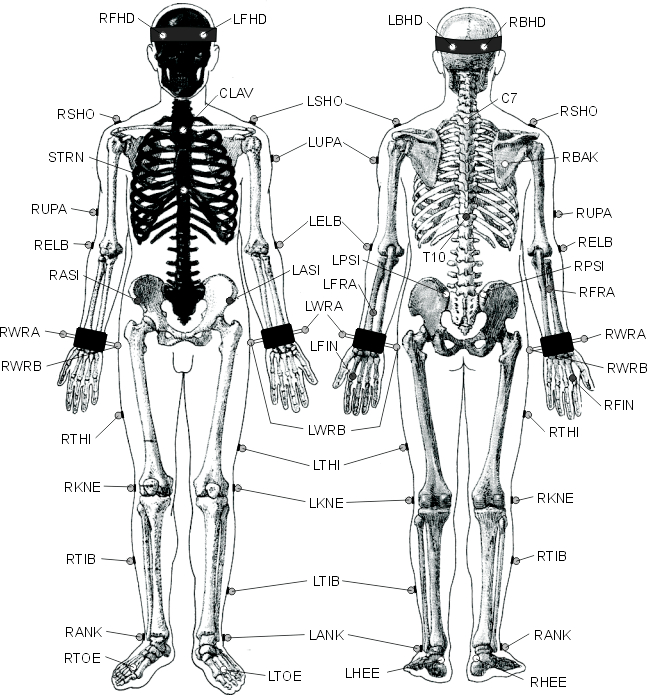
\includegraphics[width=0.75\textwidth]{images/markerPlacement.jpg}
	\caption{Rysunek przedstawiający schemat umieszczania markerów na ciele człowieka w~systemie śledzenia ruchu firmy Vicon\cite{ViconGaitPlacement}}
	\label{fig:literature:vicon:markerPlacement}
\end{figure}
		
Kolejnym krokiem po wyznaczeniu położenia poszczególnych markerów, na podstawie obrazów z~kamer, jest interpretacja tych danych w~taki sposób, aby uzyskać opis stanu stawów, które są reprezentowane graficznie przez pojedyncze punkty posiadajace informacje nie tylko o~swoim położeniu, ale także orientacji przestrzennej. Interpretacja ta odbywa się bądź to na podstawie obliczeń matematycznych, wynikających wprost z~położenia przestrzennego wyznaczonych punktów i~relacji między nimi, lub na podstawie przyjętego modelu biomechanicznego ciała ludzkiego. 
Przykładem sposobu wyznaczania położenia stawu na podstawie wzajemnej relacji pomiędzy stawami, może być proces wyznaczania położenia kości miedniczej (\emph{ang. pelvis}). Rysunek \ref{fig:literature:vicon:pelvisPlacement} pokazuje umiejscowienie markerów wykorzystywanych do wyznaczenia pozycji stawu reprezentującego kość miedniczą. Według dokumentacji \cite{ViconModelingInstruction} położenie kości miedniczej jest szacowane jako średnia arytmetyczna punktów RASI i~LASI (rys. \ref{fig:literature:vicon:pelvisPlacementA}). Jeśli jeden z~tych dwóch punktów jest niewidoczny, wówczas położenie stawu reprezentującego kość miedniczą jest wyznaczane jako wierzchołek trójkąta prostokątnego, którego przeciwprostokątną wyznaczają punkty SACR oraz jeden z~widocznych RASI lub LASI.
		
\begin{figure}
	\centering	
	\subfigure[Położenie markerów]{
		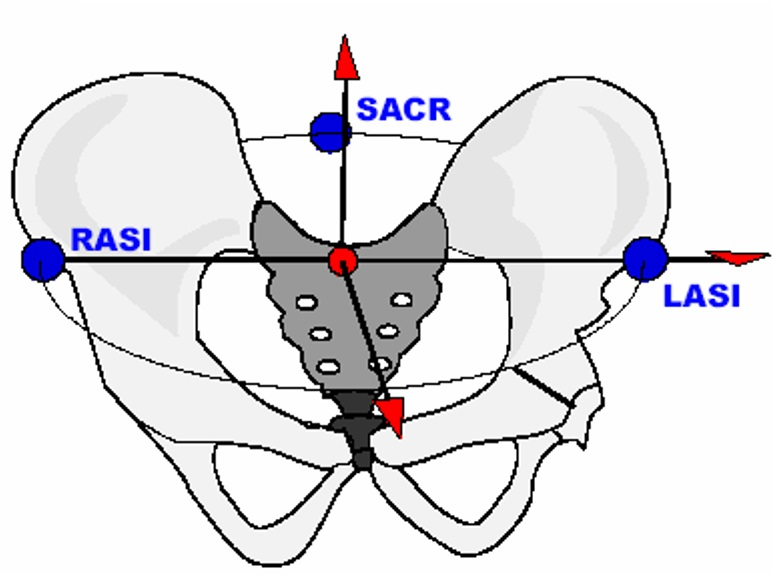
\includegraphics[width=0.45\textwidth]{images/pelvisEstimationA.jpg}
		\label{fig:literature:vicon:pelvisPlacementA}}
	\subfigure[Położenie wyznaczonego stawu kości miedniczej]{
		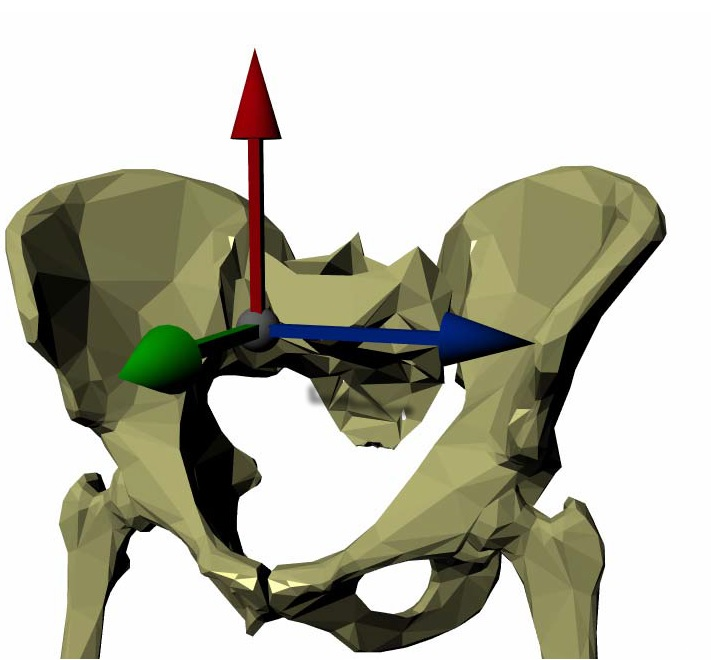
\includegraphics[width=0.45\textwidth]{images/pelvisEstimationB.jpg}	}
	\caption{Rysunek przedstawiający wyznaczenie położenia kości miedniczej na potrzeby modelu szkieletowego na podstawie położenia markerów w~systemie Vicon\cite{ViconModelingInstruction}}
	\label{fig:literature:vicon:pelvisPlacement}
\end{figure}
		
Przykładem wyznaczania położenia stawu modelu szkieletowego na podstawie biomachanicznego modelu szkieletu ludzkiego, może być schemat wyznaczania położenia stawów biodrowych. Opierając się na pracy Davies i in. \cite{Davis1991} do wyznaczenia położenia stawów zostały wykorzystane informacje o~szerokości miednicy, długości kości udowej postaci, której ruch jest śledzony, oraz współczynników skalujących i~stałych zdefiniowanych we wspomnianej pracy. Równania \eqref{eq:hipEquation:Xcoordinate}--\eqref{eq:hipEquation:Zcoordinate} przedstawiają przykład wyznaczania współrzędnych położenia dla prawego biodra.
		
\begin{subequations}
	\begin{align}
		X & = f_C * \cos(\gamma) * \sin(\upsilon) - (f_h + f_m) * \cos(\upsilon) \label{eq:hipEquation:Xcoordinate} \\
		Y & = -(f_C * \sin(\gamma) - f_a) \label{eq:hipEquation:Ycoordinate}                                        \\
		Z & = -f_C * \cos(\gamma)*\cos(\upsilon) - (f_h + f_m) * \sin(\upsilon) \label{eq:hipEquation:Zcoordinate}  
	\end{align}
	\label{eq:hipEquation:XYZcoordinates}
\end{subequations}
		
Przyjmując, że $l_l$ i~$l_p$ to długości kości udowych obu nóg, współczynnik $f_C$ zdefiniowany jest empirycznie według wzoru \eqref{eq:hipEquation:Ccoeficient}.
		
\begin{equation}
	\centering
	f_C = \frac{l_l + l_p}{2} * 0.115 - 15.3
	\label{eq:hipEquation:Ccoeficient}
\end{equation}
		
Współczynnik $f_h$ wyznaczany jest na podstawie wartości $l_l$ albo $l_p$ w~zależności czy wyznaczane jest położenie biodra dla lewej albo prawej strony. Współczynnik $f_h$ zdefiniowany został według wzoru \eqref{eq:hipEquation:Hcoeficient}.
		
\begin{equation}
	\centering
	f_h = 0.1288 * l_p - 48.56
	\label{eq:hipEquation:Hcoeficient}
\end{equation}
		
Współczynnik $f_a$ wyznaczony jest jako połowa odległości pomiędzy stawem kości miedniczej a~położeniem markera LASI albo RASI, natomiast współczynnik $f_m$ określa średnicę markerów wykorzystywanych w~trakcie śledzenia. Kąty $\gamma$ oraz $\upsilon$ przyjmują stałe wartości odpowiednio $0.5 rad$ oraz $0.314 rad$. W~dokumentacji systemu śledzenia Vicon\cite{ViconModelingInstruction} można również znaleźć opisy procedur wyznaczania położenia dla pozostałych stawów.
	
%[Fixed]cały ten podrozdział jak dla mnie jest do przepisania, bo przecież pozycję można obliczac zliczeniowo, na podstawie przyspieszeń.!!!
\subsubsection*{Wyznaczanie położenia stawów w~inercyjnych i~magnetycznych systemach śledzenia ruchu}
Inercyjne i~magnetyczne systemu śledzenia ruchu wymagają nieco innego podejścia do wyznaczania położenia poszczególnych stawów, ponieważ nie udostępniają one bezpośrednio informacji dotyczących ich położenia w~przestrzeni, a~jedynie orientację oraz wartości sił działających na poszczególne czujniki. Pozwala to określić przyspieszenie i~kierunek z~jakim porusza się czujnik (akcelerometr) oraz prędkość z~jaką się obraca (żyroskop). Dzięki wykorzystaniu pomiarów poszczególnych czujników inercyjnych, możliwe jest zastosowanie metod zliczeniowych do określenia przybliżonego położenia wynikającego z przemieszczenia się obiektu, do którego dany czujnik jest przymocowany \cite{HyeRiPark2009, Montorsi2013b}. Uzyskanie dokładnego położenia danego czujnika wymaga wykorzystania drogich komponentów, w~których zaszumienie danych pomiarowych jest stosunkowo niewielkie. W~przypadku powszechnie dostępnych czujników inercyjnych wykorzystywanych przykładowo w~telefonach, czy w~inercyjnych systemach śledzenia ruchu, takich jak XSense, czujniki inercyjne wykorzystywane są do określenia orientacji przestrzennej takiego czujnika, czy kształtu pozy jaką przyjęła w~danej chwili śledzona osoba. Konsekwencją takiego podejścia jest to, że korzeń modelu szkieletowego w~systemie śledzenia ruchu opartym o~czujniki inercyjne i~magnetyczne pozostaje zazwyczaj nieruchomy. \\
Możliwe jest zdefiniowanie tylko fragmentu modelu szkieletowego, zawierającego przykładowo ramię i~przedramię prawej ręki, którego korzeniem będzie staw barkowy. Wówczas cały model zbudowany będzie z~3 stawów, jednego nieruchomego odpowiadającego stawowi barkowemu i~dwóm ruchomym: łokciowemu i~nadgarstkowemu.\\
%[Fixed] z~powyższym akapitem się nie zgadzam, bo przecież istnieją inercyjne systemy śledzenia ruchu postaci. To trzeba przepisać.
		
W inercyjnych i~magnetycznych systemach śledzenia ruchu markery wyposażone w~odpowiednie czujniki umieszczane są na powierzchni ciała osoby (wzdłuż kości), której ruch jest śledzony. Czujniki inercyjne działają najlepiej jeśli umieszczone są blisko środka masy poruszającego się obiektu. Wyznaczeniem środków mas kości człowieka zajmują się między innymi badacze z~zakresu biomechaniki, a~przykładem efektów tych prac może być diagram wyznaczający środki mas kości zaprezentowany w~pracy Paolo de Leva \cite{DeLeva1996} i przedstawiony na rysunku \ref{fig:centerOfMass}.\\
		
\begin{figure}[!htp]
	\centering	
	\includegraphics[width=0.75\textwidth]{images/imuArm.png}
	\caption{Przykładowy schemat umieszczenia markerów inercyjnych na potrzeby śledzenia ruchu ręki.}
	\label{fig:literature:imuMarkerPlacementSample}
\end{figure}
		
Rysunek \ref{fig:literature:imuMarkerPlacementSample} pokazuje przykładowy sposób umieszczenia markerów inercyjnego systemu śledzenia ruchu na powierzchni ręki, tak aby ich położenie możliwie pokrywało się ze środkiem mas poszczególnych segmentów kończyny. 
%([Fixed] dopisałem końcówkę, ale nie wiem czy tak jest w~rzeczywistości)
Moduły inercyjne, dostarczające informacje o~swojej orientacji w~przestrzeni, 
%([Fixed] a~nie przemieszczenia? A co z~akcelerometrem?)(Kwestia przemieszczeń opisana powyżej)
nie przekazują wprost informacji o~położeniu konkretnych stawów, a~jedynie określają jaki obrót, względem jakiegoś stanu początkowego, wykonała kończyna, do której te moduły zostały przymocowane. Posługując się przykładowym schematem z~rysunku \ref{fig:literature:imuMarkerPlacementSample}, przyjmijmy staw barkowy (3) jako korzeń. Chcąc określić położenie stawu łokciowego (4), niezbędna jest informacja o~orientacji przestrzennej modułu inercyjnego umieszczonego na ramieniu (1), oraz długość kości ramieniowej, która łączy stawy barkowy i~łokciowy. Mając te dwie informacje należy dokonać obrotu wektora o~długości takiej, jak długość kości ramieniowej, do orientacji, w~jakiej znajduje się rozważany moduł (1). Wówczas punkt początkowy hierarchicznego modelu szkieletowego ręki
%([Fixed] jaki początek, czego poczatek?) 
reprezentuje staw barkowy i~znajduje się w~umownym punkcie $(0 , 0 , 0)$, natomiast punkt końcowy reprezentuje staw łokciowy, a~jego współrzędne $(X , Y , Z)$ odpowiadają położeniu tego stawu w~przestrzeni. Wyznaczenie położenia stawu nadgarstkowego (5) odbywa się analogicznie, przy czym punktem początkowym jest położenie stawu łokciowego (4), a,~modułem którego orientacja jest brana pod uwagę, jest sensor umieszczony na przedramieniu (2). W~przypadku systemów śledzenia ruchu wykorzystujących moduły inercyjne, w~których położenie stawów nie jest wyznaczane wprost z~uzyskanych pomiarów, ale mymaga dodatkowych obliczeń i~transformacji geometrycznych, istotne jest zachowanie hierarchii wykorzystywanego modelu szkieletowego i~wykonywanie obliczeń zgodnie z~tą hierarchią.\\
W przypadku konieczności budowania modelu szkieletowego na podstawie przekształceń geometrycznych, jak ma to miejsce w~przypadku inercyjnych systemów śledzenia ruchu, istotnym jest wykorzystanie odpowiedniej reprezentacji orientacji tak, aby wykonywanie obliczeń matematycznych było jak najprostsze i~dawało jednoznaczne wyniki.
		
\subsubsection*{Wyznaczanie położenia stawów modelu szkieletowego w~optycznym, bezmarkerowym systemie śledzenia ruchu}\label{chap:humanModel:kinect}
Na przykładzie kotrolera Microsoft Kinect można przedstawić jeden z~możliwych sposobów wyznaczania modelu postaci 
%([Fixed] system sledzenia nie wyznacza modelu postaci)% 
przez oprogramowanie wykorzystywane w~systemie śledzenia ruchu nie bazującym na markerach, lecz stosującym algorytmy rozpoznawania obrazów. Algorytm zastosowany w~kontrolerze Kinect jest w~stanie rozpoznać tylko szkielet postaci ludzkiej, a~w~zależności od trybu pracy szkielet ten przedstawia całą sylwetkę albo jedynie jej górną część, na którą składają się głowa, ręce oraz barki. Należy zwrócić uwagę, że model szkieletowy przedstawiający pełną sylwetkę, jest jedynie modelem uproszczonym zawierającym 20 stawów (rys. \ref{fig:characteristics:kinect:skeleton}).
		
Kontroler Kinect wykorzystuje mechanizm uczenia maszynowego, dzięki któremu możliwe jest rozpoznawanie poszczególnych części ciała śledzonej postaci na podstawie obrazu mapy głębi. Zastosowana w~kontrolerze metoda uczenia maszynowego opiera się na algorytmie losowych lasów decyzyjnych\cite{Criminisi2011}, który podlegał wcześniejszemu procesowi uczenia. W~celu nauczenia algorytmów decyzyjnych, zastosowanych w~kontrolerze Kinect, przygotowano bazę ponad miliona wzorców różnych póz, w~jakich może się znajdować śledzona postać wraz z~oznaczonymi częściami ciała. Zestaw zdjęć zastosowany do uczenia algorytmu składał się z~blisko stu tysięcy zdjęć póz rzeczywistych postaci, uzupełnionych pomiarami z~systemu śledzenia ruchu o~wysokiej dokładności oraz z~kilkuset tysięcy wzorcowych zdjęć cyfrowych postaci wygenerowanych (wyrenderowanych) komputerowo. Odpowiednio wytrenowany algorytm zyskał gotowość do rozpoznawania i~klasyfikowania elementów przedstawionego obrazu jako części ciała człowieka. Wykorzystując między innymi wzajemne położenie elementów (pojedyncze punkty lub grupy punktów -- obszary) występujących na mapie głębi 
%([Fixed] co to sa piksele występujące na mapie głębi?)
, algorytm szacuje, które z~nich należą do tej samej części ciała. Efektem działania algorytmu losowych lasów decyzyjnych jest tzw. mapa części ciała (ang. \emph{body parts map}), której przykład przedstawiony jest jako drugi krok na schemacie widocznym na rysunku \ref{fig:literature:kinect:classificationSteps}.
		
\begin{figure}[!htp]
	\centering	
	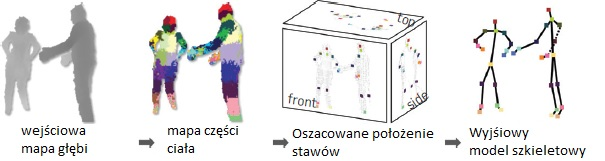
\includegraphics[width=0.75\textwidth]{images/KinectRecognitionSteps.jpg}
	\caption{Schemat przedstawiający kolejne kroki wyznaczania modelu szkieletowego na podstawie mapy głębi.}
	\label{fig:literature:kinect:classificationSteps}
\end{figure}
		
Mapa części ciała stanowi podstawę dla kolejnego kroku wyznaczania modelu szkieletowego, jakim jest oszacowanie położenia stawów w~przestrzeni trójwymiarowej. Segmenty, z~których składa się mapa części ciała, przetworzone są algorytmem \emph{mean shift} \cite{Comaniciu2003}, co w~efekcie daje oszacowanie położenia poszczególnych stawów. Połączenie ich zgodnie ze zdefiniowaną hierarchią wyznacza model szkieletowy śledzonej postaci. Warto zaznaczyć, że większość tych operacji zaimplementowana została jako oprogramowanie wbudowane procesora firmy Prime Sense.\\
%%%%%%%%%%%%%%%%%%%%%%%%%%%%%%%%%%%%%%%%%%%%%%%%%%%%%%%%%%%%%%%%%%%%%%%%%%%%%%%%%%%%%%%%%%%%		
Hipotetycznie, w~celu wykorzystania Kinecta do podobnego rozpoznawania innych obiektów czy zwierząt, należałoby zaimplementować powyżej przedstawiony proces opierając się na specjalnie przygotowanych do tego danych.
Warto zwrócić uwagę, że proces wyznaczania mapy głębi i~reprezentacji szkieletowej śledzonego użytkownika opiera się na danych pozyskanych tylko z~jednego układu jaki stanowią kamera i~projektor światła podczerwonego (IR - ang. \textit{infra red}). Kamera RGB nie jest w~ogóle do tego zadania wykorzystywana, co z~kolei skutkuje tym, że urządzenie jest w~stanie działać w~zaciemnionych pomieszczeniach.\\
		
Kinect wykorzystuje reprezentację ciała użytkownika w~postaci szkieletowej. Składa się ona z~20 jednopunktowych węzłów, które w~dużej mierze pokrywają się ze stawami ludzkiego szkieletu (rys. \ref{fig:characteristics:kinect:skeleton}). Każdy z~węzłów posiada swoje współrzędne w~przestrzeni trójwymiarowej związanej z~kontrolerem wyrażone w~metrach, gdzie punktem (0,0,0) jest projektor podczerwieni w~kontrolerze Kinect. Rysunek \ref{fig:characteristics:kinect:space} przedstawia układ współrzędnych wykorzystywany w~Kinekcie do określenie położenia stawów. 
		
\begin{figure}
	\centering
	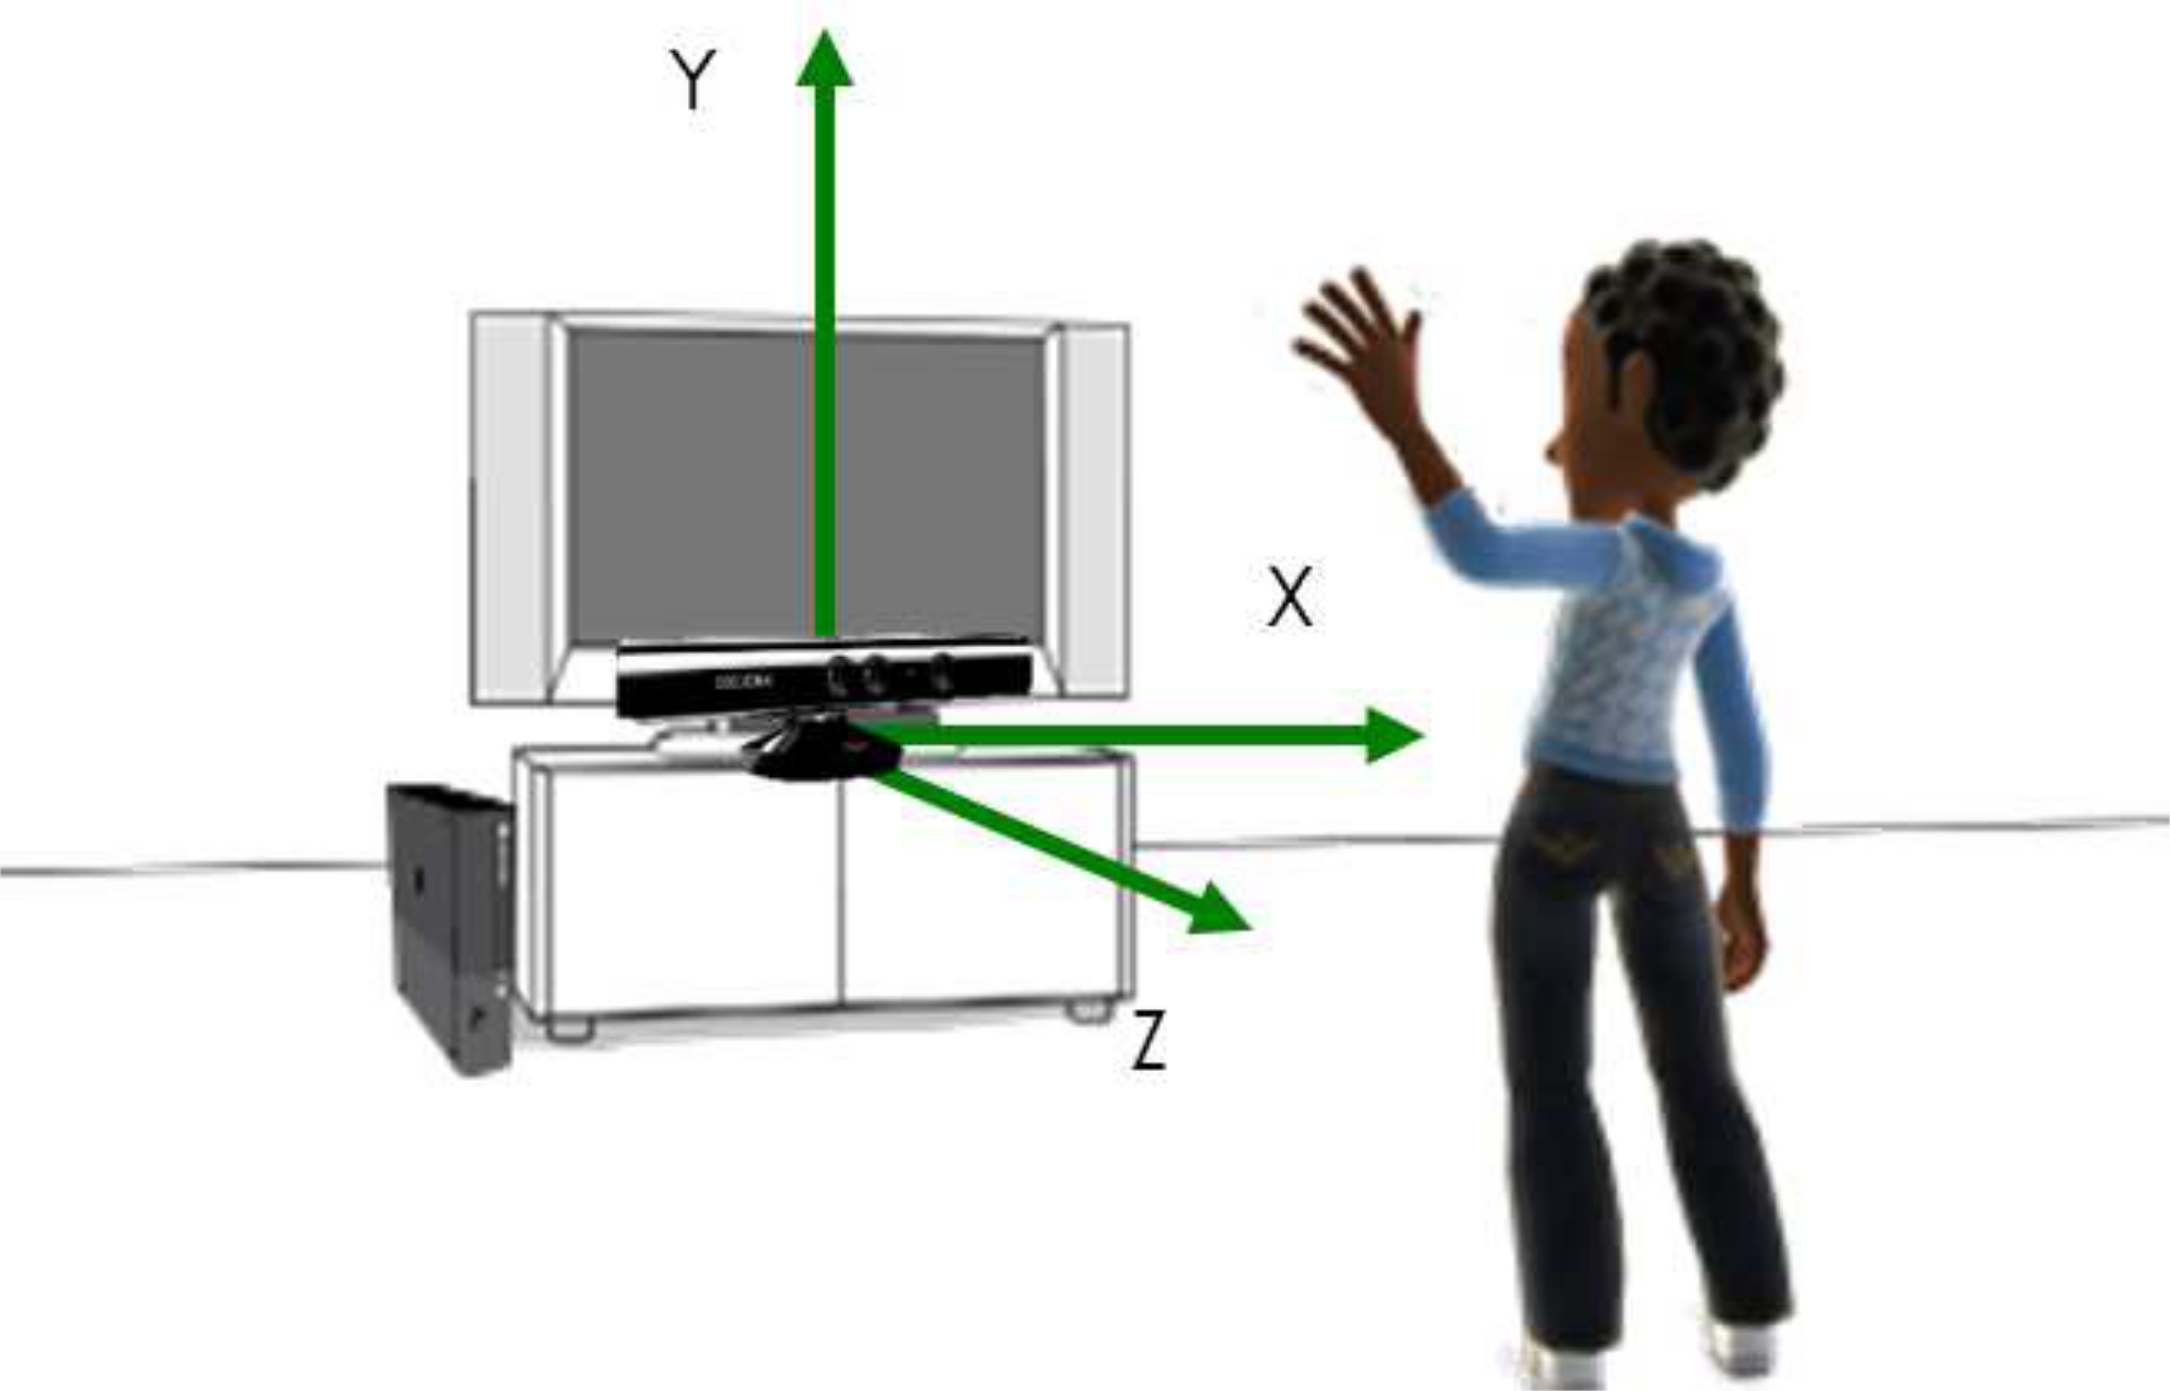
\includegraphics[width=0.6\textwidth]{images/skeletonSpace.png}
	\caption{Układ współrzędnych wykorzystywany w~kontrolerze Microsoft Kinect \cite{msdn:kinectCoordSpace2016}}
	\label{fig:characteristics:kinect:space}
\end{figure}
		

\subsection{Reprezentacja rotacji obiektu w~przestrzeni}\label{chap:orientstionRep}
Istnieje wiele metod reprezentowania jak zorientowany w~przestrzeni jest obiekt i~każda z~tych metod wyróżnia się charakterystycznymi dla siebie cechami, które na przykład mogą wpływać na łatwość obliczeń kosztem czytelności zapisu czy optymalizacją użycia pamięci w~ich implementacji komputerowej. Do najpopularniejszych można zaliczyć następujące metody:
	
\begin{itemize}
	\item Kąty Eulera
	\item Macierze rotacji
	\item Para Osie-Kąt (\emph{ang. Axis--Angle})
	\item Kwaterniony
\end{itemize} 
		
\subsubsection*{Kąty Eulera} \label{sec:orientstionRep:euler}
Reprezentacja ta jest najbardziej intuicyjną z~powszechnie używanych, ponieważ przedstawia ona 3 wartości kątów o~jakie nastąpił obrót względem odpowiednich osi układów współrzędnych. W~zależności od dziedziny w~jakiej określana jest orientacja obiektu, przyjęta jest nieco inna konwencja nazewnicza poszczególnych kątów. Jest to związane z~układem odniesienia jaki jest przyjęty do określania obrotów: relatywny, w~którym obrót mierzony jest względem arbitralnie wybranego układu (\emph{body--fixed coordinate system}, rys.\ref{fig:appx:rot:eulerRel}) lub absolutny względem kierunków ziemi (\emph{ang. world coordinate system}, rys.\ref{fig:appx:rot:eulerAbs}). Tabela \ref{tab:appx:rot:eulerNames} zawiera powszechnie przyjęte konwencje oznaczania obrotów.
		
\begin{figure}
	\centering
	\subfigure[Relatywny \cite{nasa2016}]{
		\label{fig:appx:rot:eulerRel}
		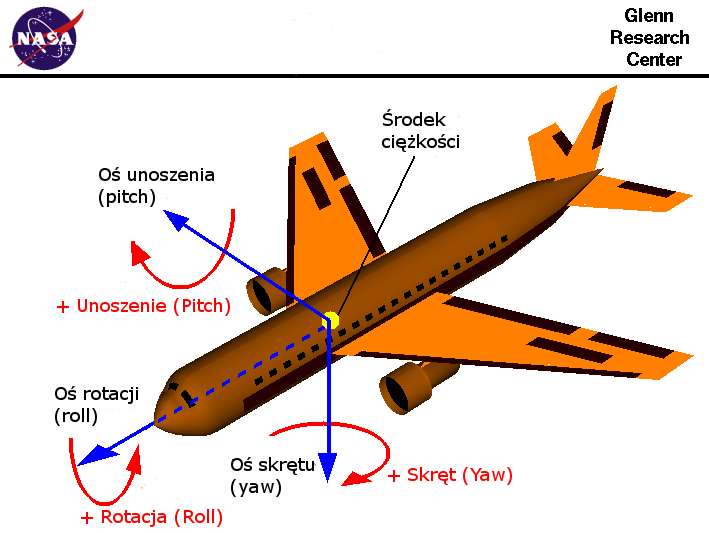
\includegraphics[width=0.75\textwidth]{images/nasaAircraft.png}
	}
														
	\subfigure[Absolutny \cite{Baker2015}]{
		\label{fig:appx:rot:eulerAbs}
		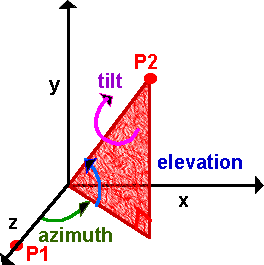
\includegraphics[width=0.5\textwidth]{images/eulerAbsolute.png}	
	}
															
	\caption{Kąty Eulera względem przyjętego układu współrzędnych}
\end{figure}
		
\begin{table}
	\centering
	\caption{Konwencje nazewnicze kątów Eulera}
	\label{tab:appx:rot:eulerNames} 
	\begin{tabular}{|c|c|c|c|c|}
		\hline
		Oś & Układ Relatywny & Układ Absolutny & Symbol   & Prędkość kątowa \\
		\hline
		X   & \emph{bank}      & \emph{tilt}      & $\psi$   & \emph{roll}         \\
		Y   & \emph{heading}   & \emph{azimuth}   & $\theta$ & \emph{yaw}          \\ 
		Z   & \emph{attitude}  & \emph{elevation} & $\phi$   & \emph{pitch}        \\
		\hline
	\end{tabular} 
\end{table}
		
Chcąc prawidłowo interpretować podane wartości trzeba pamiętać, że określają one zawsze obroty względem określonych osi w~ściśle określonej sekwencji. Spośród 27 możliwych kombinacji określających kolejność wykonywania rotacji (osie w~sekwencji mogą się powtarzać), jedynie 12 może być wykorzystane do zdefiniowania obrotów w~przestrzeni 3D. Dokładne opisy sekwencji wykonywanych obrotów można znaleźć w~pracach poświęconych zagadnieniu rotacji obiektów np. \cite{Pio1966, Diebel2006}. Innym utrudnieniem, które trzeba brać pod uwagę w~przypadku stosowania kątów Eulera jest występowanie niejednoznaczności przy obrotach w~pozycji pionowej ($ \phi=90\degree $). W~takim wypadku wykonanie dowolnej innej rotacji powoduje niejednoznaczność względem której osi odbył się ruch. Sytuacja o~której jest mowa nosi angielską nazwę \emph{gimbal lock}. W~przypadku implementacji komputerowej, taki przypadek wymaga szczególnej obsługi w~celu uniknięcia błędów zarówno interpretacyjnych jak i~stricte matematycznych.
		
\subsubsection*{Macierze orientacji}
Reprezentacja w~postaci kątów Eulera jest intuicyjna w~interpretacji przez człowieka, ale utrudnia ona obliczanie obrotów na bieżąco. W~takim przypadku należy ją skonwertować do innej postaci -- dobrze sprawdzają się tu macierze obrotów względem każdej z~osi, opisane wzorami \eqref{eq:appx:rot:rMatrix:rx}, \eqref{eq:appx:rot:rMatrix:ry} oraz \eqref{eq:appx:rot:rMatrix:rz}.
		
\begin{subequations}
	\begin{align}
		\mathbf{R_x(\alpha)} & = 
		\begin{bmatrix}
		1            & 0            & 0            \\
		0            & cos(\alpha)  & sin(\alpha)  \\
		0            & -sin(\alpha) & cos(\alpha)  
		\end{bmatrix} 
		\label{eq:appx:rot:rMatrix:rx} \\				
		\mathbf{R_y(\alpha)} & = 
		\begin{bmatrix}
		cos(\alpha)  & 0            & -sin(\alpha) \\
		0            & 1            & 0            \\
		sin(\alpha)  & 0            & cos(\alpha)  
		\end{bmatrix} 
		\label{eq:appx:rot:rMatrix:ry} \\				
		\mathbf{R_z(\alpha)} & = 
		\begin{bmatrix}
		cos(\alpha)  & sin(\alpha)  & 0            \\
		-sin(\alpha) & cos(\alpha)  & 0            \\
		0            & 0            & 1            
		\end{bmatrix} 
		\label{eq:appx:rot:rMatrix:rz}
	\end{align}
\end{subequations}
		
Rotacja o~dowolne kąty względem każdej z~osi rozumiana jest jako iloczyn powyższych macierzy. Końcowa postać macierzy obrotu będąca wynikiem takiego iloczynu wyrażona jest wzorem \eqref{eq:appx:rot:rMatrix:all}.
		
\begin{equation}
	\footnotesize
	\begin{split}
		&\mathbf{R(\phi,\theta,\psi)} = \mathbf{R_z(\psi)}\mathbf{R_y(\theta)}\mathbf{R_x(\phi)} =\\
		&=	\begin{bmatrix}
		cos(\theta)cos(\psi)   & cos(\phi)sin(\psi) + cos(\phi)sin(\theta)cos(\psi) & sin(\phi)sin(\psi) - cos(\phi)sin(\theta)cos(\psi) \\
		-cos(\theta)sin(\psi)  & cos(\phi)cos(\psi) - sin(\phi)sin(\theta)sin(\psi) & sin(\phi)cos(\psi) + cos(\phi)sin(\theta)sin(\psi) \\
		sin(\theta)            & 			-sin(\phi)cos(\theta) 		            & cos(\phi)cos(\theta)            
		\end{bmatrix} 
		\label{eq:appx:rot:rMatrix:all}
	\end{split}
\end{equation}
			
\subsubsection*{Para Osie-Kąt (\emph{ang. Axis--Angle})}
Reprezentacja w~postaci pary Osie-Kąt odpowiada za określenie kierunku (osie) oraz wielkość obrotu (kąt). Zapisuje się ją jak we wzorze \eqref{eq:appx:rot:angleAxis:form}
	
\begin{equation}
	\alpha\mathbf{e} = (\alpha, \begin{bmatrix}e_1 & e_2 & e_3\end{bmatrix})
	\label{eq:appx:rot:angleAxis:form}
\end{equation}
		
przy założeniu, że wektor $\mathbf{e}$ jest wektorem o~długości 1. 
Forma ta jest zbliżona do reprezentacji kwaternionowej, jednak nie można używać jej w~obliczeniach z~podobną łatwością.  
		
\subsubsection*{Kwaterniony}
Ostatnią z~prezentowanych reprezentacji orientacji są kwaterniony. Są to liczby z~ciała liczb zespolonych złożony z~części rzeczywistej reprezentowanych przez jedną liczbę oraz części urojonej na która składają się 3 pozostałe. Jej zaletą jest łatwość i~zwięzłość zapisu operacji obrotu obiektu oraz składania sekwencji obrotów. Obarczone jest to jednak utrudnioną interpretacją tego zapisu przez człowieka. Aby na podstawie kwaternionu określić pod jakim kątem w~stosunku do osi poszczególnych znajduje się obiekt, należy dokonać szeregu operacji arytmetycznych. Ogólna postać kwaternionu wyrażona jest jak we wzorze \eqref{eq:appx:rot:quat}:
		
\begin{equation}
	\label{eq:appx:rot:quat}
	\mathbf{q} =
	\begin{bmatrix}
		q_0 \\
		q_1 \\
		q_2 \\
		q_3 
	\end{bmatrix} 
	= 	
	\begin{bmatrix}
		q_w \\
		q_x \\
		q_y \\
		q_z 
	\end{bmatrix} 
	= 
	\begin{bmatrix}
		cos(\frac{\alpha}{2})    \\
		e_1sin(\frac{\alpha}{2}) \\
		e_2sin(\frac{\alpha}{2}) \\
		e_3sin(\frac{\alpha}{2}) 
	\end{bmatrix}
\end{equation}
gdzie $q_{0-1}, q_{w-z}, e_{1-3} \in \mathbb{R}, \alpha \in [-\pi \pi], \sqrt{e_1^2 + e_2^2 + e_3^2} = 1$
		
Wartości kąta $\alpha$ oraz $e_{1-3}$ są tożsame z~reprezentacją w~postaci Osie-Kąt.
		
Wzór \eqref{eq:appx:rot:quat} nie wyczerpuje wszystkich reprezentacji kwaternionów jakie występują w~literaturze, widać na nim jednak, że określenie o~ile stopni obrócono obiekt jest przynajmniej trudne. Wybierając dowolną notację dla kwaternionów, ze względu na ich mnogość, należy szczególnie zadbać o~określenie, która z~wartości w~wektorze odpowiada za część rzeczywistą tej liczby, a~które za część urojoną. Niesprecyzowanie tej informacji może skutkować błędami w~interpretacji podczas obliczeń. W~niniejszej pracy część rzeczywista reprezentowana jest przez element wektora oznaczony indeksem $0$ lub $w$. Wzór \eqref{eq:appx:rot:quat} pokazuje też związek pomiędzy kwaternionem a~reprezentacją w~postaci pary Osie-Kąt.
		
Aby skutecznie dokonywać obliczeń za pomocą kwaternionów muszą być one znormalizowane, czyli spełniać zależność $\|\mathbf{q}\| = 1$
		
Opis operacji matematycznych oraz geometrycznych jakie wykonywane mogą być na kwaternionach można znaleźć w~szeregu publikacji (np. \cite{Dantam2014}) na ten temat, a~także w~podręcznikach akademickich dotyczących matematyki.
		
\subsubsection*{Konwersje}
W każdej z~powyższych reprezentacji istnieje możliwość dokonania konwersji na dowolną inną. Taka operacja może być przydatna jeśli chcemy np. prezentować aktualną orientację obiektu użytkownikowi, a~postać, która jest używana przy obliczeniach nie jest łatwa do interpretacji przez człowieka. Z~uwagi na to, że w~niniejszej pracy do wyrażenia orientacji i~obrotów wykorzystane były dwie formy prezentacji: kąty Eulera oraz kwaterniony, konwersja pomiędzy tymi dwoma typami została przedstawiona poniżej.
		
\subsubsection*{Kąty Eulera $\rightarrow$ Kwaternion}
Przyjmując, że kąty Eulera wyrażone sa przez sekwencję obrotów $Z-Y-X$ (\emph{Tait–Bryan angles}) konwersja z~kątów Eulera do kwaternionów wyrażona jest wzorem \eqref{eq:appx:rot:eulerToQuat}
		
\begin{equation}
	\label{eq:appx:rot:eulerToQuat}
	\begin{bmatrix}
		q_w \\
		q_x \\
		q_y \\
		q_z 
	\end{bmatrix} 
	= 
	\begin{bmatrix}
		\cos{\frac{\psi}{2}}\cos{\frac{\theta}{2}}\cos{\frac{\phi}{2}}+\sin{\frac{\psi}{2}}\sin{\frac{\theta}{2}}\sin{\frac{\phi}{2}} \\
		\cos{\frac{\psi}{2}}\cos{\frac{\theta}{2}}\sin{\frac{\phi}{2}}-\sin{\frac{\psi}{2}}\sin{\frac{\theta}{2}}\cos{\frac{\phi}{2}} \\
		\cos{\frac{\psi}{2}}\sin{\frac{\theta}{2}}\cos{\frac{\phi}{2}}+\sin{\frac{\psi}{2}}\cos{\frac{\theta}{2}}\sin{\frac{\phi}{2}} \\
		\sin{\frac{\psi}{2}}\cos{\frac{\theta}{2}}\cos{\frac{\phi}{2}}-\cos{\frac{\psi}{2}}\sin{\frac{\theta}{2}}\sin{\frac{\phi}{2}} 
	\end{bmatrix}
\end{equation}
		
\subsubsection*{Kwaternion $\rightarrow$ Kąty Eulera}
Przy analogicznych założeniach co do sekwencji kątów Eulera, konwersja z~postaci kwaternionowej wyrażona jest wzorem \eqref{eq:appx:rot:quatToEuler}
		
\begin{equation}	
	\label{eq:appx:rot:quatToEuler}
	\begin{matrix}
		\begin{matrix}                                                   
		\theta = arcsin(-2(q_x q_z-q_w q_y))                             \\
		\psi = arctan2((q_y q_z + q_w q_x), \frac{1}{2}-(q_x^2 + q_y^2)) \\
		\phi = arctan2((q_x q_y + q_w q_z), \frac{1}{2}-(q_y^2 + q_z^2)) 
	\end{matrix} & \quad \text{if } 2(q_x q_z-q_w q_y) \ne \pm 1 \\
	& \\	
	& \\
	\begin{matrix}
		\theta = \frac{-\pi}{2}                                         \\
		\phi + \psi = arctan2((q_x q_y - q_w q_z), (q_x q_z + q_w q_y)) 
	\end{matrix} & \quad \text{if } 2(q_x q_z-q_w q_y) = +1 \\
	& \\	
	& \\
	\begin{matrix}
		\theta = \frac{\pi}{2}                                          \\
		\phi - \psi = arctan2((q_x q_y - q_w q_z), (q_x q_z + q_w q_y)) 
	\end{matrix} & \quad \text{if } 2(q_x q_z-q_w q_y) = -1 
	\end{matrix}
\end{equation}
		
\section{Charakterystyka wykorzystywanych urządzeń pomiarowych}\label{chap:characteristics}
W niniejszej pracy zostały wykorzystane dwa typy urządzeń: kamera RGB-D w~postaci kontrolera ruchu Microsoft Kinect dla konsoli gier Microsoft XBox 360 oraz inercyjne czujniki ruchu (ang. \emph{Inertial Measurement Unit - IMU}): akcelerometr i~żyroskop. Ich powszechna dostępność sprawiła, że zagadnienie śledzenia ruchu ciała ludzkiego przestało być zarezerwowane jedynie dla profesjonalistów dysponujących drogim i~bardzo rozbudowanym systemem śledzenia oraz rejestrowania ruchu (ang. \emph{Motion Capture}, MoCap). Korzystając z~obu typów urządzeń należy zwrócić szczególną uwagę na charakterystykę ich działania oraz ograniczenia takie jak wrażliwość na okluzje sensora głebi, niedokładność pomiarów, czy wręcz ich brak, dla niektórch stopni swobody czujników inercyjnych. Świadomość ta jest niezbędna przy budowaniu algorytmów śledzenia ruchu w~oparciu o~wymienione urządzenia. 
		
\subsection{Kontroler Microsoft Kinect v. 1}\label{sec:characteristics:kinect}
Pierwsza wersja kontrolera ruchu Microsoft Kinect została oficjalnie udostępniona do sprzedaży rynkowej w~2010 roku (wcześniej prezentowano prototypy pod nazwą kodową "Project Natal"). Urządzenie to stało się pierwszym, powszechnie dostępnym, kontrolerem śledzącym ruch użytkownika bez wykorzystywania markerów, który odniósł faktyczny sukces komercyjny\footnote{W lutym 2013 łączna sprzedaż kontrolera Microsoft Kinect osiągnęła 24 miliony sztuk \cite{kinectSales2013}}.  
		
\subsubsection*{Budowa kontrolera}
Śledzenie ruchu za pomocą tego urządzenia oparte jest o~system wizyjny zbudowany z~dwóch kamer z~matrycami CMOS oraz z~projektora światła podczerwonego. Jedna z~kamer odpowiada za rejestrowanie tradycyjnego obrazu RGB, natomiast druga, wraz z~projektorem, tworzy sensor głębi, który potrafi określić, w~jakiej odległości od Kinecta znajdują się obiekty na scenie. Obie kamery działają z~częstotliwością nie przekraczającą 30 fps (ang. \textsl{frames per second}). Ponadto urządzenie posiada cztery mikrofony, a~głównym komponentem odpowiedzialnym za przetwarzanie i~interpretację zarejestrowanych obrazów wejściowych jest dedykowany procesor opracowany i~wyprodukowany przez izraelską firmę Prime Sense. Firma ta jest także autorem algorytmu rozpoznającego ruchy i~gesty użytkownika na podstawie zarejestrowanych przez kamery sygnałów wejściowych. Rysunek \ref{fig:characteristics:kinect:inside} przedstawia uproszczony schemat budowy tego kontrolera. 
		
\begin{figure}
	\centering
	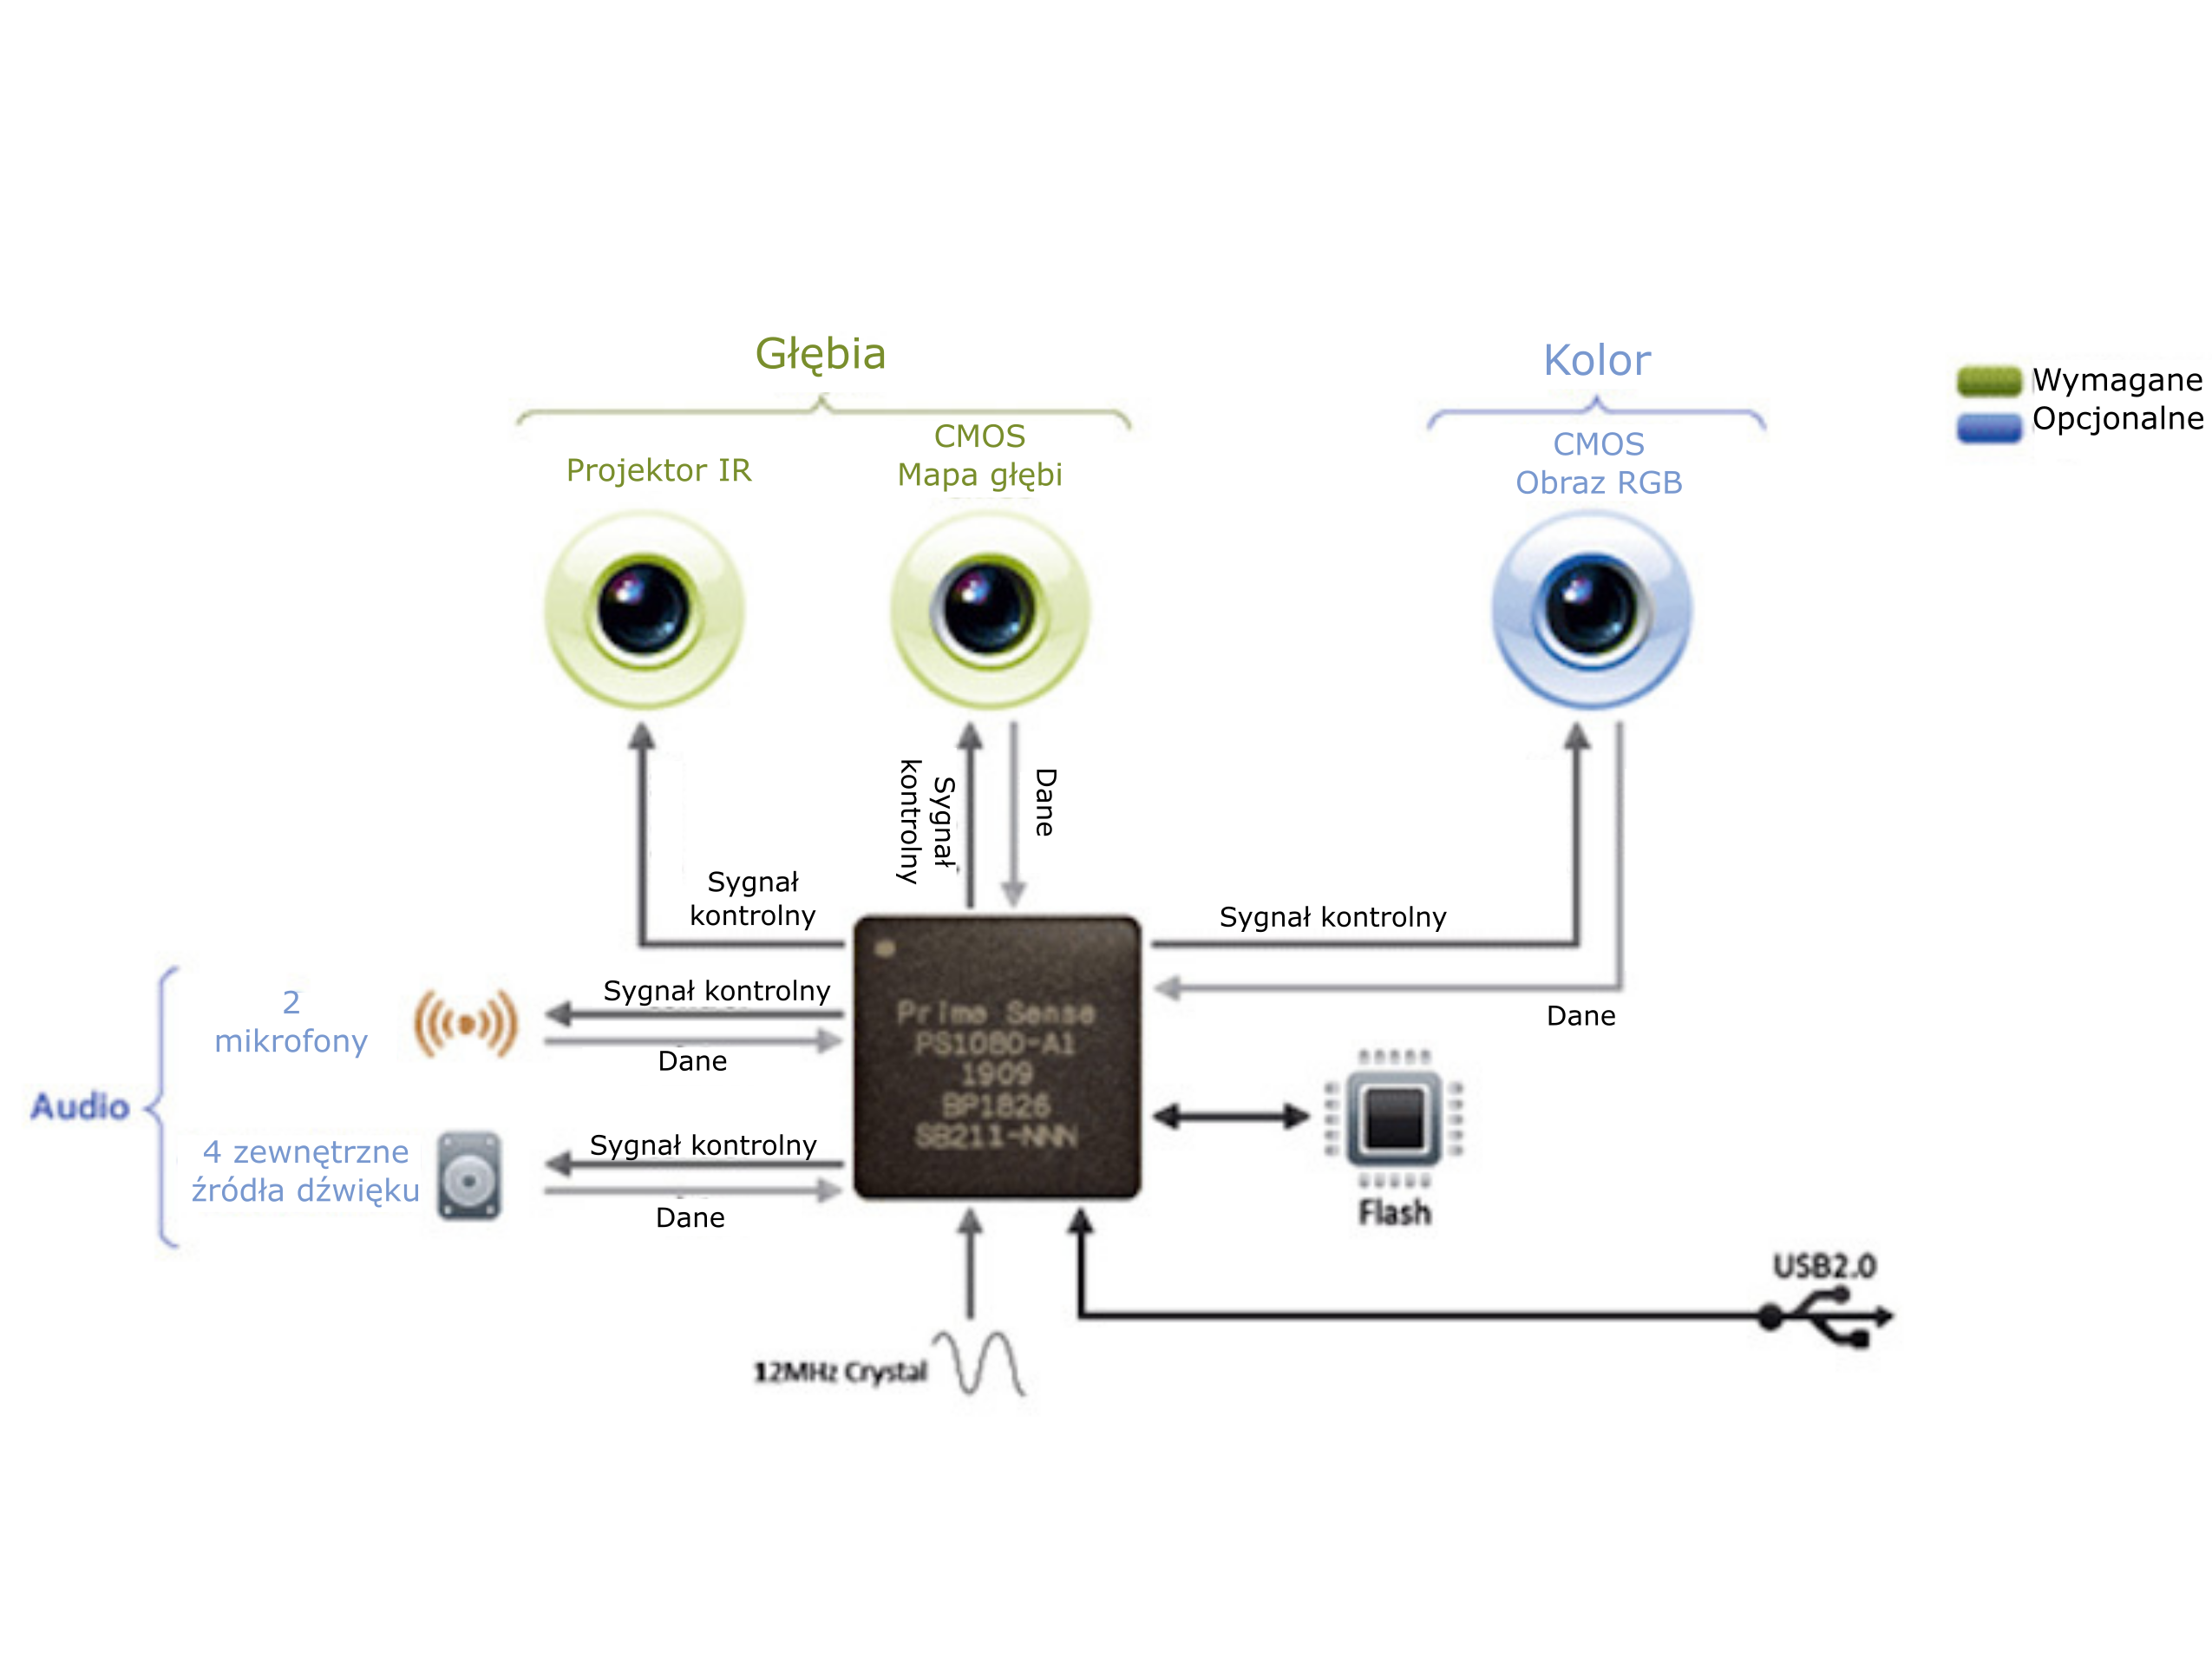
\includegraphics[width=0.95\textwidth]{images/kinectSchema.png}
	\caption{Uproszczony schemat budowy kontrolera Microsoft Kinect v.1 \cite{kinectFixit2016}}
	\label{fig:characteristics:kinect:inside} 
\end{figure}
		
Według oficjalnej dokumentacji \cite{kinectSpec2016} Kinect pracuje poprawnie, gdy obiekt (postać) znajduje się w~odległości od $0.8m$ do $4m$ od urządzenia oraz zawiera się w~polu widzenia urządzenia: $57\degree$ w~orientacji poziomej i~$43\degree$ w~orientacji pionowej. Oficjalny zakres pracy urządzenia przedstawia rysunek \ref{fig:characteristics:kinect:range}. Dla odległości mniejszej niż $0.4m$ i~większej niż $8m$ Kinect nie zwraca żadnych wyników pozwalających określić czy jakiś obiekt znajduje się przed nim czy nie. Oficjalna dokumentacja nie zawiera jednak informacji o~ewentualnej niejednorodności precyzji działania w~obszarze pracy. Można by więc przypuszczać, że urządzenie działa jednakowo precyzyjnie w~dowolnym miejscu znajdującym się w~zakresie roboczym urządzenia \footnote{Eksperymenty badawcze weryfikujące to przypuszczenie zostały zawarte w~dalszej części niiejszego rozdziału \ref{sssection:distanceEstimation}}. 
%([Fixed] podać w~któreym rozdziale)
Specyfikacja udostępniona na stronach MSDN \footnote{MSDN -- \emph{\textbf{M}icro\textbf{s}oft \textbf{D}eveloper \textbf{N}etwork}, portal internetowy zawierający dokumentacje i~poradniki głownie dla programistów korzystających z~produktów i~narzędzi firmy Microsoft. dostępny pod adresem \url{http://https://msdn.microsoft.com}}
%([Fixed] wprowadzić przypis dolny i~wyjasnić co to jest MSDN) 
przedstawia prawdopodobnie pewien uśredniony lub minimalny zakres pracy, ponieważ zgodnie z~obserwacjami użytkowników \cite{stack:kinect2011} oraz badaniami porównawczymi \cite{DiFilippo2015} okazuje się, że poszczególne serie produkcyjne urządzenia mogą mieć nieco inne zakresy pracy. Występowanie różnic w~zakresie działania pomiędzy poszczególnymi egemplarzami kontrolera Kinect zostało także przewidziane w~oficjalnym SDK przygotowanym przez firmę Microsoft\cite{msdn:kinectSDKConstants2016}. Analizując kod źródłowy SDK urządzenia można zauważyć rozbieżność pomiędzy dokumentacją dotyczącą maksymalnych zakresów działania, a~faktyczną implementacją. Jako przykład można podać wartość kąta widzenia kamery urządzenia w~pionie: według dokumentacji wynosi on $43\degree$, natomiast faktyczna implementacja podaje różne wartości dla kamer głębi i~RGB, a~wynoszą one odpowiednio $45.6\degree$ i~$48.6\degree$. 
		
\begin{savenotes}
	\begin{figure}[hbp]
		\centering
		\begin{subfigure}[b]{0.5\textwidth}
			\centering
			
\begin{tikzpicture}[scale=0.4]					
	\draw[very thin,pattern=dots, pattern color = black] (61.5:0.8) -- (61.5:4) arc (61.5:118.5:4) -- (118.5:0.8) arc (118.5:61.5:0.8) -- cycle;						
	\draw[very thin,pattern=horizontal lines, pattern color = black] (61.5:4) -- (61.5:8) arc (61.5:118.5:8) -- (118.5:4) arc (118.5:61.5:4) -- cycle;						
	\draw[very thin,fill=black!10] (61.5:8) -- (61.5:9) arc (61.5:118.5:9) -- (118.5:8) arc (118.5:61.5:8) -- cycle;
																																										
	\draw[dashed, very thin,fill=black!10] (61.5:8) -- (61.5:9) arc (61.5:0:9) -- (0:8) arc (0:61.5:8) -- cycle;
	\draw[dashed, very thin,fill=black!10] (61.5:4) -- (61.5:8) arc (61.5:0:8) -- (0:4) arc (0:61.5:4) -- cycle;
	\draw[dashed, very thin,fill=black!10] (61.5:0.8) -- (61.5:4) arc (61.5:0:4) -- (0:0.8) arc (0:61.5:0.8) -- cycle;
	\draw[dashed, very thin,fill=black!10] (61.5:0.4) -- (61.5:0.8) arc (61.5:0:0.8) -- (0:0.4) arc (0:61.5:0.4) -- cycle;
	\draw[dashed, very thin,fill=black!10] (61.5:0) -- (61.5:0.4) arc (61.5:0:0.4) -- (0:0) arc (0:61.5:0) -- cycle;
																																										
	\draw[dashed, very thin,fill=black!10] (118.5:8) -- (118.5:9) arc (118.5:180:9) -- (180:8) arc (180:118.5:8) -- cycle;
	\draw[dashed, very thin,fill=black!10] (118.5:4) -- (118.5:8) arc (118.5:180:8) -- (180:4) arc (180:118.5:4) -- cycle;
	\draw[dashed, very thin,fill=black!10] (118.5:0.8) -- (118.5:4) arc (118.5:180:4) -- (180:0.8) arc (180:118.5:0.8) -- cycle;
	\draw[dashed, very thin,fill=black!10] (118.5:0.4) -- (118.5:0.8) arc (118.5:180:0.8) -- (180:0.4) arc (180:118.5:0.4) -- cycle;
	\draw[dashed, very thin,fill=black!10] (118.5:0) -- (118.5:0.4) arc (118.5:180:0.4) -- (180:0) arc (180:118.5:0) -- cycle;
																																										
																																										
	\draw[very thin,fill=black!10] (0:0) -- (61.5:0.4) arc (61.5:118.5:0.4) -- (0:0);
																																																							
	\draw[fill=black] (0, 0) circle (0.15);
																																																								
	\draw (0:0.4) node[below right, rotate=-45] {$0.4m$};
	\draw (0:1.2) node[below right, rotate=-45] {$0.8m$};
	\draw (0:4) node[below right, rotate=-45] {$4m$};		
	\draw (0:8) node[below right, rotate=-45] {$8m$};			
	\draw (0:9) node[below right, rotate=-45] {$9m$};
																																																													
	\draw[<->, thin, black] (65:6) arc (65:115:6);
	\draw[black] (80.5: 6) node[above] {$57^\circ$};
																																																						
	\draw (61.5: 9.5) node {$28.5^\circ$};
	\draw (118.5: 9.5) node {$28.5^\circ$};
	\draw[thick, ->] (90:0) -- (90:9.5);
																																																										
	\draw (90: 10) node {Kierunek obserwacji};
\end{tikzpicture}
			\caption{Horyzontalny zakres pracy}
			\label{fig:kinect:range:a}
		\end{subfigure} \hfill
		\begin{subfigure}[b]{0.5\textwidth}
			\centering
			\begin{tikzpicture}[scale=0.45]
	\draw[very thin,pattern=dots, pattern color = black] (-21.5:0.8) -- (-21.5:4) arc (-21.5:21.5:4) -- (21.5:0.8) arc (21.5:-21.5:0.8) -- cycle;
	\draw[very thin,pattern=horizontal lines, pattern color = black] (-21.5:4) -- (-21.5:8) arc (-21.5:21.5:8) -- (21.5:4) arc (21.5:-21.5:4) -- cycle;
	\draw[very thin,fill=black!10] (-21.5:8) -- (-21.5:9) arc (-21.5:21.5:9) -- (21.5:8) arc (21.5:-21.5:8) -- cycle;
	\draw[very thin,fill=black!10] (-21.5:0) -- (-21.5:0.4) arc (-21.5:21.5:0.4) -- (21.5:0) arc (21.5:-21.5:0) -- cycle;
	\draw[very thin,fill=white] (-21.5:0.4) -- (-21.5:0.8) arc (-21.5:21.5:0.8) -- (21.5:0.4) arc (21.5:-21.5:0.4) -- cycle;
																																																									
	\draw[fill=black] (0, 0) circle (0.15);
	\draw[thick, ->] (0:0) -- (0:9.5);
	\draw (0: 10) node[right] {Kierunek obserwacji};
	% 																																				
	\draw[<->, thin, black] (-18:4.3) arc (-18:18:4.3);
	\draw[black] (-15: 4.3) node[right] {$43^\circ$};
	% 																																				
	\draw[->, thin, black, dashed] (0:6.5) arc (0:-10:6.5);
	\draw[black] (-10: 6.5) node[right] {$-21.5^\circ$};
	% 																																				
	\draw[->, thin, black, dashed] (0:6.5) arc (0:10:6.5);
	\draw[black] (10: 6.5) node[right] {$+21.5^\circ$};
	% 																										
	\draw (0:0) node[left] {Kinect}		;				
	\draw (20.5:0.4) node[above] {$0.4m$};
	\draw (33.5:1.2) node[above] {$0.8m$};
	\draw (21.5:4) node[above] {$4m$};		
	\draw (21.5:8) node[above] {$8m$};			
	\draw (21.5:9) node[above] {$9m$};
																																																									
\end{tikzpicture}
			\caption{Wertykalny zakres pracy}
			\label{fig:kinect:range:b}
		\end{subfigure} \hfill
		\begin{subfigure}[p]{\textwidth}
			\hfill
			\begin{tikzpicture}[scale=0.1]	
	\node[draw=black,thick,rounded corners=2pt,below left=2mm] {%
		\begin{tabular}{@{}r@{ }l@{}}
			\raisebox{2pt}{\tikz{\draw[black!10, fill=black!10] (0,0) rectangle (5mm,2mm);}}                               & Niewidoczne                       \\
			\raisebox{2pt}{\tikz{\draw[black,pattern=dots, pattern color = black] (0,0) rectangle (5mm,2mm);}} & Za daleko                         \\
			\raisebox{2pt}{\tikz{\draw[black, fill=black] (0,0) rectangle (5mm,2mm);}}                                     & Za blisko                         \\
			\raisebox{2pt}{\tikz{\draw[black,fill=white] (0,0) rectangle (5mm,2mm);}}             & Obszar roboczy                    \\
			\raisebox{2pt}{\tikz{\draw[<->, thin] (0:0) arc (0:180:0.3);}}                                                 & Zakres pracy                      \\
			\raisebox{2pt}{\tikz{\draw[<-, thin, dashed] (0:0) arc (0:180:0.3);}}                                          & Przesunięcie kierunku obserwacji \\
			\raisebox{2pt}{\tikz{\draw[fill=black] (0, 0) circle (0.15);}}                                                 & Kinect                            
		\end{tabular}};	
\end{tikzpicture}		
               
		\end{subfigure}
							
		\caption[Horyzontalny i wertykalny zakres pracy kontrolera Microsoft Kinect v.1]{Horyzontalny (a) i wertykalny (b) zakres pracy kontrolera Microsoft Kinect v.1 (na podstawie \footfullcite{footnote:kinectSpec2016})}
		\label{fig:characteristics:kinect:range}	
	\end{figure}
\end{savenotes} 
		
\subsubsection*{Wyznaczanie mapy głębi}
Sposób w~jaki Kinect określa odległość w~jakiej umieszczone są przed nim obiekty opiera się o~rozpoznawanie zniekształceń ściśle zdefiniowanego wzorca świetlnego, którym została oświetlona scena (ang. \emph{structured light}). W~tym procesie biorą udział jedynie projektor oraz kamera IR, natomiast obraz z~kamery RGB nie jest wykorzystywany na żadnym etapie określania odległości. Technika ta jest wykorzystywana powszechnie przykładowo w~skanerach 3D \cite{david2016,lmi2016}. Dokładne działanie kontrolera Kinect nie zostało oficjalnie ujawnione publicznie przez firmę Microsoft. Możliwe jest jednakże przedstawienie przybliżonego działania tego kontrolera dzięki niezależnym badaniom (np. MacCormick \cite{MacCormick2011}) oraz analizie zgłoszeń patentowych \cite{patent:20080106746,patent:20100020078,patent:20100118123} należących do producenta procesora wykorzystanego do budowy kontrolera Kinect -- firmy Prime Sense.
		
W pierwszym kroku cała scena zostaje oświetlona zbiorem punktów za pomocą projektora światła podczerwonego (rys. \ref{fig:characteristics:kinect:nightVision}) zgodnie ze ściśle określonym wzorcem (rys. \ref{fig:characteristics:kinect:dotPattern}). Wzorzec ten nie został nigdy oficjalnie opublikowany przez firmy Prime Sense, czy Microsoft, natomiast wzorzec zamieszczony na rysunku \ref{fig:characteristics:kinect:dotPattern} został wyznaczony przez Andreasa Reichingera, doktoranta na Uniwersytecie Technicznym w~Wiedniu. Na swoim blogu opublikował on dokładny opis sposobu wyznaczania zamieszczonego wzorca\cite{reichinger2011}.
		
\begin{figure}
	\centering
	\begin{minipage}[b]{0.48\linewidth}
		\centering   
		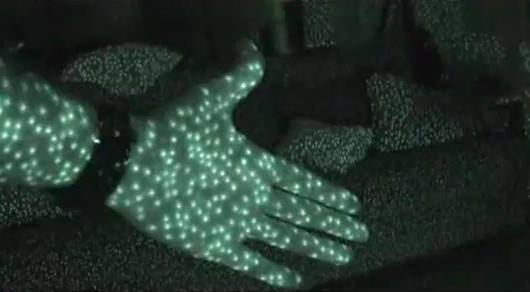
\includegraphics[width=\textwidth]{images/kinectNightVision.jpg}	
		\caption{Scena oświetlona promieniami IR\cite{flatley2011}}
		\label{fig:characteristics:kinect:nightVision}
	\end{minipage}
	\begin{minipage}[b]{0.48\linewidth}
		\centering 
		
\includegraphics[width=\textwidth]{images/kinect-pattern_3x3.png}
		\caption{Wzorzec oświetlenia sceny przez kontroler Kinect \cite{reichinger2011}}
		\label{fig:characteristics:kinect:dotPattern}
	\end{minipage}	
\end{figure}
		
Pełen wzorzec zbudowany jest z~9 powtarzających się regionów w~układzie 3x3 o~rozmiarze 211x165 punktów co daje pełen rozmiar 633x495 punktów. Około $11\%$ z~tych punktów jest jasna przy czym jasność ta nie jest jednorodna. Wyraźnie można zauważyć, że część punktów jest jaśniejsza od pozostałych. Ponadto w~punkcie centralnym każdego z~regionów (jak i~całego wzorca) znajduje się najjaśniejszy z~punktów. Dodatkowo wzorzec ten jest skośnie symetryczny, co oznacza niewrażliwość na obrócenie urządzenia~o~$180\degree$.\\
		
Następnym krokiem jest wyznaczenie mapy głębi na podstawie analizy zniekształcenia wyświetlonego wzorca. Opierając się na badaniach prowadzonych przez MacCormicka \cite{MacCormick2011}, analiza zniekształcenia wzorca opiera się na dwóch technikach:
		
\begin{itemize}
	\item wyznaczenie głębi na podstawie ostrości punktów,
	\item wyznaczenie głębi na podstawie zjawiska paralaksy.
\end{itemize}
		
Pierwsza z~technik opiera się na fakcie, że obraz obiektów umieszczonych bliżej soczewki jest mniej wyostrzony od tych znajdujących się dalej. Dodatkowo soczewki umieszczone w~kamerze IR Kinecta posiadają różną ogniskową dla osi ''x'' i~''y'', co sprawia, że okrągłe punkty stają się eliptyczne z~pochyleniem zależnym od głębokości w~jakiej znajduje się dany obiekt. Druga z~zastosowanych technik opiera się na zjawisku paralaksy, które występuje w~wyniku przesunięcia pomiędzy projektorem światła podczerwonego a~kamerą wyposarzoną w~filtr światła o~takiej częstotliwości. Szczegółowe opisy działania obu technik można znaleźć w~wielu publikacjach naukowych m.in.: Rzeszotarski, Strumiłło et al. \cite{Rzeszotarski2006} czy Fofi, Sliwa, Voisin \cite{Fofi2004}. Informacje uzyskane na podstawie obu powyższych technik są następnie ze sobą łączone w~celu uzyskania mapy głębi.
		
\subsubsection*{Ograniczenia w~działaniu kontrolera Kinect}\label{ssec:characteristics:kinect:limitation}
		
Kinect przez ponad 5 lat dostępności na rynku jest obiektem badań związanych zarówno z~jego zastosowaniem i~poprawą działania jak i~dokładnym opisaniem jego cech, oszacowaniu dokładności oraz zdefiniowaniu ograniczeń. 
		
\paragraph*{Oświetlenie sceny}
Jednym z~podstawowych ograniczeń jakie występują w~tym urządzeniu jest wrażliwość na światło słoneczne. Jak to zostało wcześniej opisane, jedynym źródłem danych wykorzystywanym do budowy mapy głębi, a~także do stworzenia modelu szkieletowego jest kamera z~filtrem podczerwieni oraz wzorzec punktów podczerwonych emitowanych przez wbudowany projektor. Światło słoneczne natomiast składa się z~pełnego spektrum barw zarówno z~zakresu widzialnego jak i~niewidzialnego dla człowieka. Oznacza to, że promienie słoneczne mogą wprowadzić dodatkowe punkty na scenie, które nie należą do wzorca, a~będą zarejestrowane przez kamerę. Zarejestrowanie przez kamerę podczerwoną kontrolera Kinect punktów spoza przyjętego wzorca prowadzi do niepoprawnego zbudowania mapy głębi wykorzystywanej w~procesie wyznaczania modelu szkieletowego. Rysunek \ref{fig:characteristics:kinect:depthMap} przedstawia mapę głębi zbudowaną wewnątrz pomieszczenia \ref{fig:characteristics:kinect:depthMapA} oraz na zewnątrz w~dwóch przypadkach, w~miejscu zacienionym \ref{fig:characteristics:kinect:depthMapB} oraz w~pełnym słońcu \ref{fig:characteristics:kinect:depthMapC}. 
		
\begin{figure}
	\subfigure[Wewnątrz pomieszczenia]{
		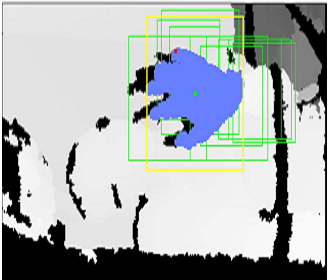
\includegraphics[width=0.3\textwidth]{images/kinectIndoor.png}
		\label{fig:characteristics:kinect:depthMapA}}
	\subfigure[Na zewnątrz pomieszczenia w~cieniu]{
		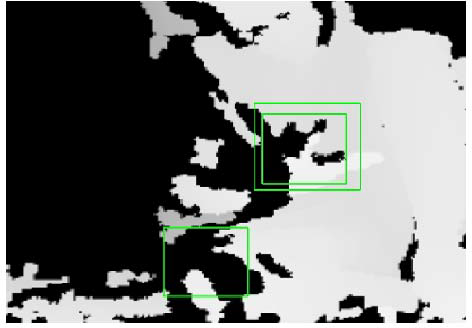
\includegraphics[width=0.3\textwidth]{images/kinecOutdoorShade.png}
		\label{fig:characteristics:kinect:depthMapB}}
	\subfigure[Na zewnątrz pomieszczenia w~świetle słonecznym]{
		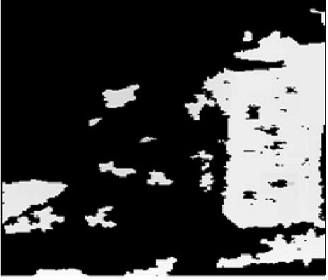
\includegraphics[width=0.3\textwidth]{images/kinecOutdoorFull.png}
		\label{fig:characteristics:kinect:depthMapC}}
	\caption{Mapa głębi ręki w~różnych warunkach oświetleniowych\cite{Suarez2012}.}
	\label{fig:characteristics:kinect:depthMap}
\end{figure}
		
Jak widać na przykładzie z~rysunku \ref{fig:characteristics:kinect:depthMap}, Kinect nie był w~stanie zbudować prawidłowej mapy w~przypadku oświetlenia sceny światłem słonecznym. \\
Z podobnych względów niezalecane jest używanie wielu Kinectów do śledzenia ruchu na jednej scenie. Co prawda SDK wspiera wykorzystanie aż 4 urządzeń równocześnie, jednak zgodnie z~oficjalną dokumentacją może to negatywnie wpłynąć na dokładność rozpoznawania części ciała, a~przez to wyznaczenia modelu szkieletowego i~śledzenia ruchu stawów \cite{msdn:multipleKinectsSDK2016}. Należy jednak wspomnieć, że scenariusz wykorzystania wielu kontrolerów Microsoft Kinect w~przypadku jednej sceny jest jednym z~obszarów badawczych wśród naukowców i~po zastosowaniu odpowiednich algorytmów m.in.  wspomagających proces kalibracji i~synchronizacji \cite{Kohno2013}, czy wprowadzających elementy uczenia maszynowego (rozpoznawanie szkieletu z~wykorzystaniem klasyfikator HCRF - ang. \emph{Hidden-state Conditional Random Fields }) \cite{Kitsikidis2011}. Badając możliwości wykorzystania kilku kontrolerów Kinect do obserwacji jednej sceny badacze byli w~stanie także poprawić działanie systemu śledzenia z~wykorzystaniem jednego urządzenia np. Asteriadis \cite{Asteriadis2013} oraz Baek \cite{Baek2014} opisali metody wykorzystania dwóch kontrolerów Kinect, dzięki którym zmniejszyli oni podatność prezentowanego systemu śledzenia na występowanie okluzji, a~przez to tracenia możliwości śledzenia ruchu stawów. To z~kolei przekłada się na dokładność oszacowania położenia stawów. Shroeder \cite{Schroder2011} zaproponował natomiast metodę poprawiającą jakość wyznaczonej mapy głębi. Według opublikowanych danych zminiejszył on liczbę pikseli niepoprawnie określających głębię z~około $20\%$ do $1\%$.
		
\paragraph*{Niepełna informacja o~obrotach}
Pozycja każdego stawu opisana jest w~kartezjańskim układzie współrzędnych w~prestrzenie trójwymiarowej przez trójkę liczb pozwalających określić jednoznacznie położenie tego stawu. Układ współrzędnych kontrolera Kinect zakłada, że jego początkiem (punkt $(0, 0, 0)$) jest kontroler, a~wszystkie udestpnione przez niego pomiary są pomiarami względnymi w~stosunku do tego niego. W~reprezentacji szkieletowej, jaką udostępnia Kinect, przyjęte jest, że z~każdym stawem powiązany jest tylko jeden punkt w~przestrzeni. Dodatkowo każdy staw jest powiązany ze swoim sąsiednim stawem tworząc kości. Mając dwa punkty położone w~przestrzeni jesteśmy w~stanie określić kierunek obrotu danej kości jednak jest to informacja ograniczona jedynie do dwóch wymiarów wyłączając obrót wokół własnej osi. Spowodowane jest to utożsamieniem każdego ze stawów z~pojedynczym punktem przestrzeni.
		
\paragraph*{Okluzje}
Innym ograniczeniem jakie należy wziąć pod uwagę jest zasłanianie stawów śledzonej postaci. Okluzja może wystąpić z~dwóch powodów:
\begin{itemize}
	\item przysłonięcie przez obiekty znajdujące się na scenie np. meble,
	\item przysłonięcie przez inne części ciała.
\end{itemize}
		
W tym miejscu należy wspomnieć o~informacji przypisanej do każdego ze stawów określającej stan jego śledzenia. Informacja ta może przyjąć jedną z~3 wartości:
\begin{itemize}
	\item \emph{Tracked} -- wartość kiedy dany staw jest w~pełni widoczny i~śledzony bez żadnych znaczących zakłóceń;
	\item \emph{Interferred} -- wartość kiedy Kinect nie jest w~stanie śledzić danego stawu, ale na podstawie innych wartości jest w~stanie oszacować jego położenie. Algorytm jakim w~tej sytuacji posługuje się Kinect do szacowania położenia nie został opublikowany;
	\item \emph{NotTracked} -- wartość kiedy dany staw jest zupełnie niewidoczny i~nie ma możliwości podania nawet jego przybliżonego położenia;
\end{itemize}
		
W praktyce, najczęściej położenie stawów jest oznaczone jako \emph{Interferred}, co oznacza, że należy dodatkowo weryfikować otrzymane dane zanim zostaną użyte, np. czy położenie danego stawu pomiędzy kolejnymi pomiarami jest prawdopodobne, czy wystąpił jednak błąd szacowania. Sposobem na taką weryfikację może być wyznaczenie stopnia przesunięcia danego stawu pomiędzy kolejnymi pomiarami. Przy częstotliwości akwizycji danych przez kontroler Kinect, która wynosi 30 klatek na sekundę, czas jaki mija pomiędzy dwiema kolejnymi klatkami to około 30ms. Tak krótki czas sprawia, że przesunięcia stawów przy normalnym ruchu postaci są realnie niewielkie, więc jeśli wyznaczone przesunięcie będzie wynosiło np. 1 metr, istnieje duże prawdopodobieństwo, że położenie stawu zostało oszacowane błędnie.\\
		
Szczególne przypadki okluzji występują, gdy użytkownik skieruje wyprostowaną kończynę w~kierunku kamery Kinecta lub obróci się cała jego sylwetka względem płaszczyzny obserwacji kontrolera Kinect. Analizując pierwszy scenariusz najłatwiej przedstawić go na przykładzie ruchu ręki. Trzymając ją na wprost kamery kontrolera Kinect, wyprostowaną w~łokciu, w~pełni widoczny jest tylko staw nadgarstkowy, a~także dłoń. Praktycznie całkowitemu przysłonięciu ulegają zaś łokieć i~staw barkowy. 
		
\begin{figure}[!htb]
	\centering
	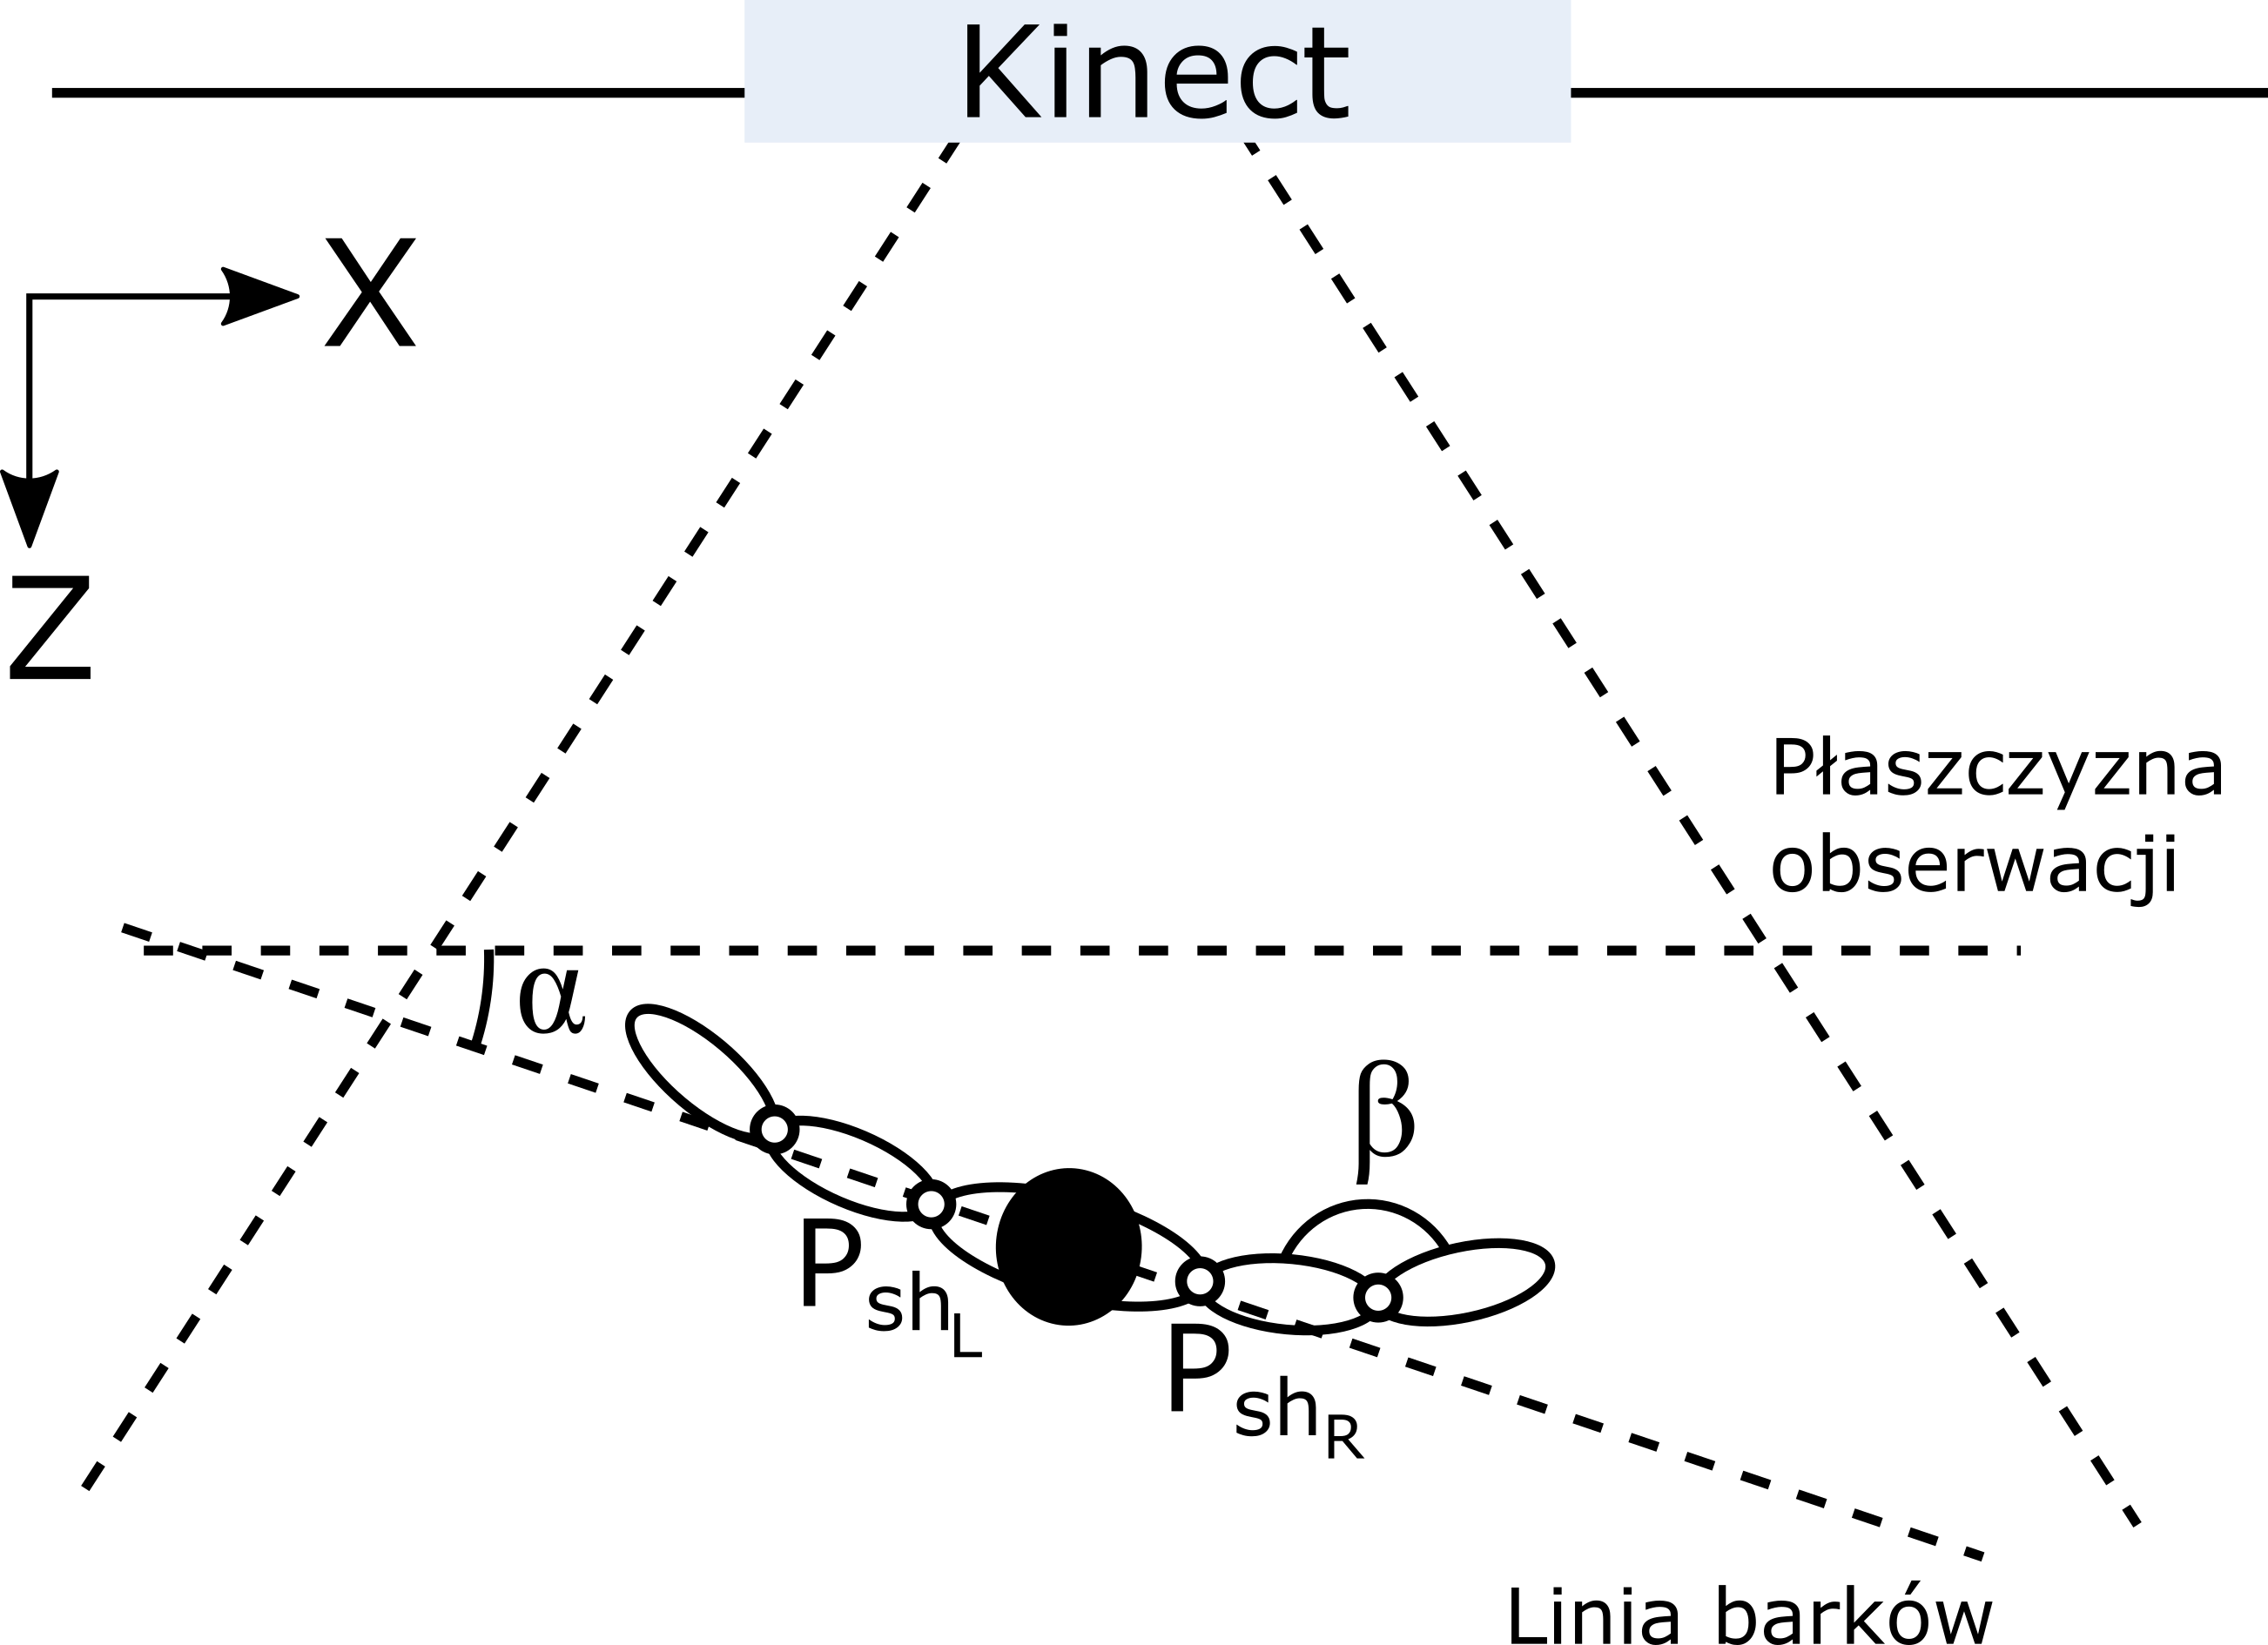
\includegraphics[width=0.5\textwidth]{images/kinectAngle.png}
	\caption{Kąt obrotu użytkownika względem Kinecta}
	\label{fig:characteristics:kinect:bodyRotationAngle}
\end{figure}
		
W trakcie badań własnych przeprowadzony został eksperyment, którego celem było oszacowanie przy jakim kącie obrotu ciała śledzonej postaci względem kontrolera Kinect następuje praktyczna utrata zdolności śledzenia przez kontroler. Eksperyment polegał na obracaniu się postaci wokół własnej osi w~tzw. pozycji \emph{T--pose}, co oznacza, obie ręce wyprostowane w~łokciach i~wyprostowane w~bok, tak że sylwetka przypomina literę "`T"'. W~trakcie wykonywania ruchu mierzony był kąt obrotu $\alpha$ pomiędzy linią barków ($P_{{Sh}_L, P_{{Sh}_R}}$) a~płaszczyzną obserwacji (rys. \ref{fig:characteristics:kinect:bodyRotationAngle}). Kąt ten jest wyznaczony w~przestrzeni dwuwymiarowej i~wyrażony jest wzorem \eqref{eq:characteristics:kinect:bodyRotationAngle}. Wszystkie współrzędne użyte w~tym wzorze wyrażone są w~układzie współrzędnych Kinecta (rys. \ref{fig:characteristics:kinect:space}).
%([Fixed] znowu sa wprowadzone jakies współrzędne do szkieletu i~wydaje mi się, że te współórzędne dla stawów szkieletu są przy kazdym rysunku inne. Warto by to sprawdzić i~ujednolicić)
	
\begin{equation}
	\label{eq:characteristics:kinect:bodyRotationAngle}
	\begin{split}
		\alpha &= 
		\begin{cases} 
			atan(\frac{|p^K_{{Sh}_R,Z} - p^K_{{Sh}_L,Z}|}{|p^K_{{Sh}_R,X} - p^K_{{Sh}_L,X}|} & , |p^K_{{Sh}_R,X} - p^K_{{Sh}_L,X}| \neq 0 \\
			\frac{\Pi}{2}                                                                    & , |p^K_{{Sh}_R,X} - p^K_{{Sh}_L,X}| = 0    \\		
		\end{cases}
	\end{split}
\end{equation}
gdzie:
\begin{conditions}
	p^K_{{Sh}_L,X}, p^K_{{Sh}_L,Z}			& współrzędne pobrane z~kontrolera Kinect określające położenie lewego barku użytkownika w~osiach X i~Z,\\
	p^K_{{Sh}_R,X}, p^K_{{Sh}_R,Z}			& współrzędne pobrane z~kontrolera Kinect określające położenie prawego barku użytkownika w~osiach X i~Z.\\
\end{conditions}
		
		
W wyniku eksperymentu okazało się, że przy kącie obrotu $\alpha$ powyżej $50\degree$ kontroler Kinect traci z~pola widzenia blisko połowę stawów użytkownika, a~to z~kolei powoduje, że pomiar wszystkich pozostałych stawów staje się niewiarygodny. Objawia się to dużymi różnicami w~oszacowaniu pozycji stawów pomiędzy dwoma kolejnymi pomiarami. Co ciekawe, różnice te są także zauważalne dla stawów oznaczonych jako \emph{Tracked}, czyli teoretycznie takich, które są w~pełni widoczne dla kontrolera. Na tej podstawie można wysunąć dwa wnioski. Po pierwsze wyznaczenie pozycji poszczególnych stawów odbywa się z~wykorzystaniem informacji o~pozostałych stawach. W~innym przypadku stawy oznaczone jako \emph{Tracked} zawsze byłyby pozycjonowane w~poprawny sposób. Drugi wniosek jaki się nasuwa dotyczy póz wykorzystywanych jako zestaw uczący dla algorytmu losowych lasów decyzyjnych (rozdział \ref{chap:humanModel:kinect}). Pozy wykorzystywane do nauczenia Kinecta prawidłowego rozpoznawania części ciała człowieka przedstawiają prawdopodobnie postać stojącą na wprost, względnie obruconą w~niewielkim stopniu do płaszczyzny obserwacji. Stąd problemy kontrolera Kinect w~określaniu położenia nawet widocznych stawów w~sytuacji gdy śledzona postać jest obrócona.\\
		
Wykres na rysunku \ref{fig:characteristics:kinect:bodyRotationChart} przedstawia status śledzenia lewego i~prawego barku (linie przerywane) w~zależności od kąta obrotu $\alpha$ wyznaczonego na podstawie pomiarów Kinecta (linia ciągła). Stan śledzenia stawu \emph{Tracked} reprezentowany jest przez wartość liczbową $1$ (wartość na prawej osi pionowej) natomiast stan \emph{Interferred} przez wartość $0.5$. Obrót wykonywany był w~kierunku przeciwnym do ruchu wskazówek zegara co oznacza, że prawa strona ciała była cały czas widoczna dla urządzenia śledzącego ruch. Jak widać na tym wykresie, przy kącie zbliżonym do $50\degree$ status śledzenia zaczyna zmieniać się gwałtownie, aby ustalić swoją wartość po przekroczeniu rzeczonego kąta. W~przedziale od $50\degree$ do $90\degree$ można zaobserwować duże wahania pomiaru, co jest spowodowane błędnym szacowaniem położenia lewego barku.\\ 
Wykres przedstawiony na rysunku \ref{fig:characteristics:kinect:kinectRightHandElbowAngle} pokazuje również zmianę wartości kąta mierzonego w~łokciu prawej ręki $\beta$ (rys. \ref{fig:characteristics:kinect:bodyRotationAngle}) w~trakcie wykonywania obrotu. Ręka przez cały czas trwania obrotu była wyprostowana w~łokciu i~stanowiła przedłużenie linii pomiędzy barkami (\emph{T--pose}). Jak widać na wykresie, pomimo pełnej widoczności prawej ręki przez kamery Kinecta przy obrocie w~zakresie  $50\degree < \alpha \le 90\degree$ , pomiar kąta $\beta$ jest niestabilny, a~jego wartość nie jest nawet zbliżona do wartości kąta wyprostowanej w~łokciu ręki ($170\degree-180\degree$). 
		
\begin{figure}  [!htp] 
	\begin{center}
		\subfigure[Stan śledzenia stawów podczas obrotu ciała \emph{(T-pose)} względem kontrolera]{\label{fig:characteristics:kinect:bodyRotationChart}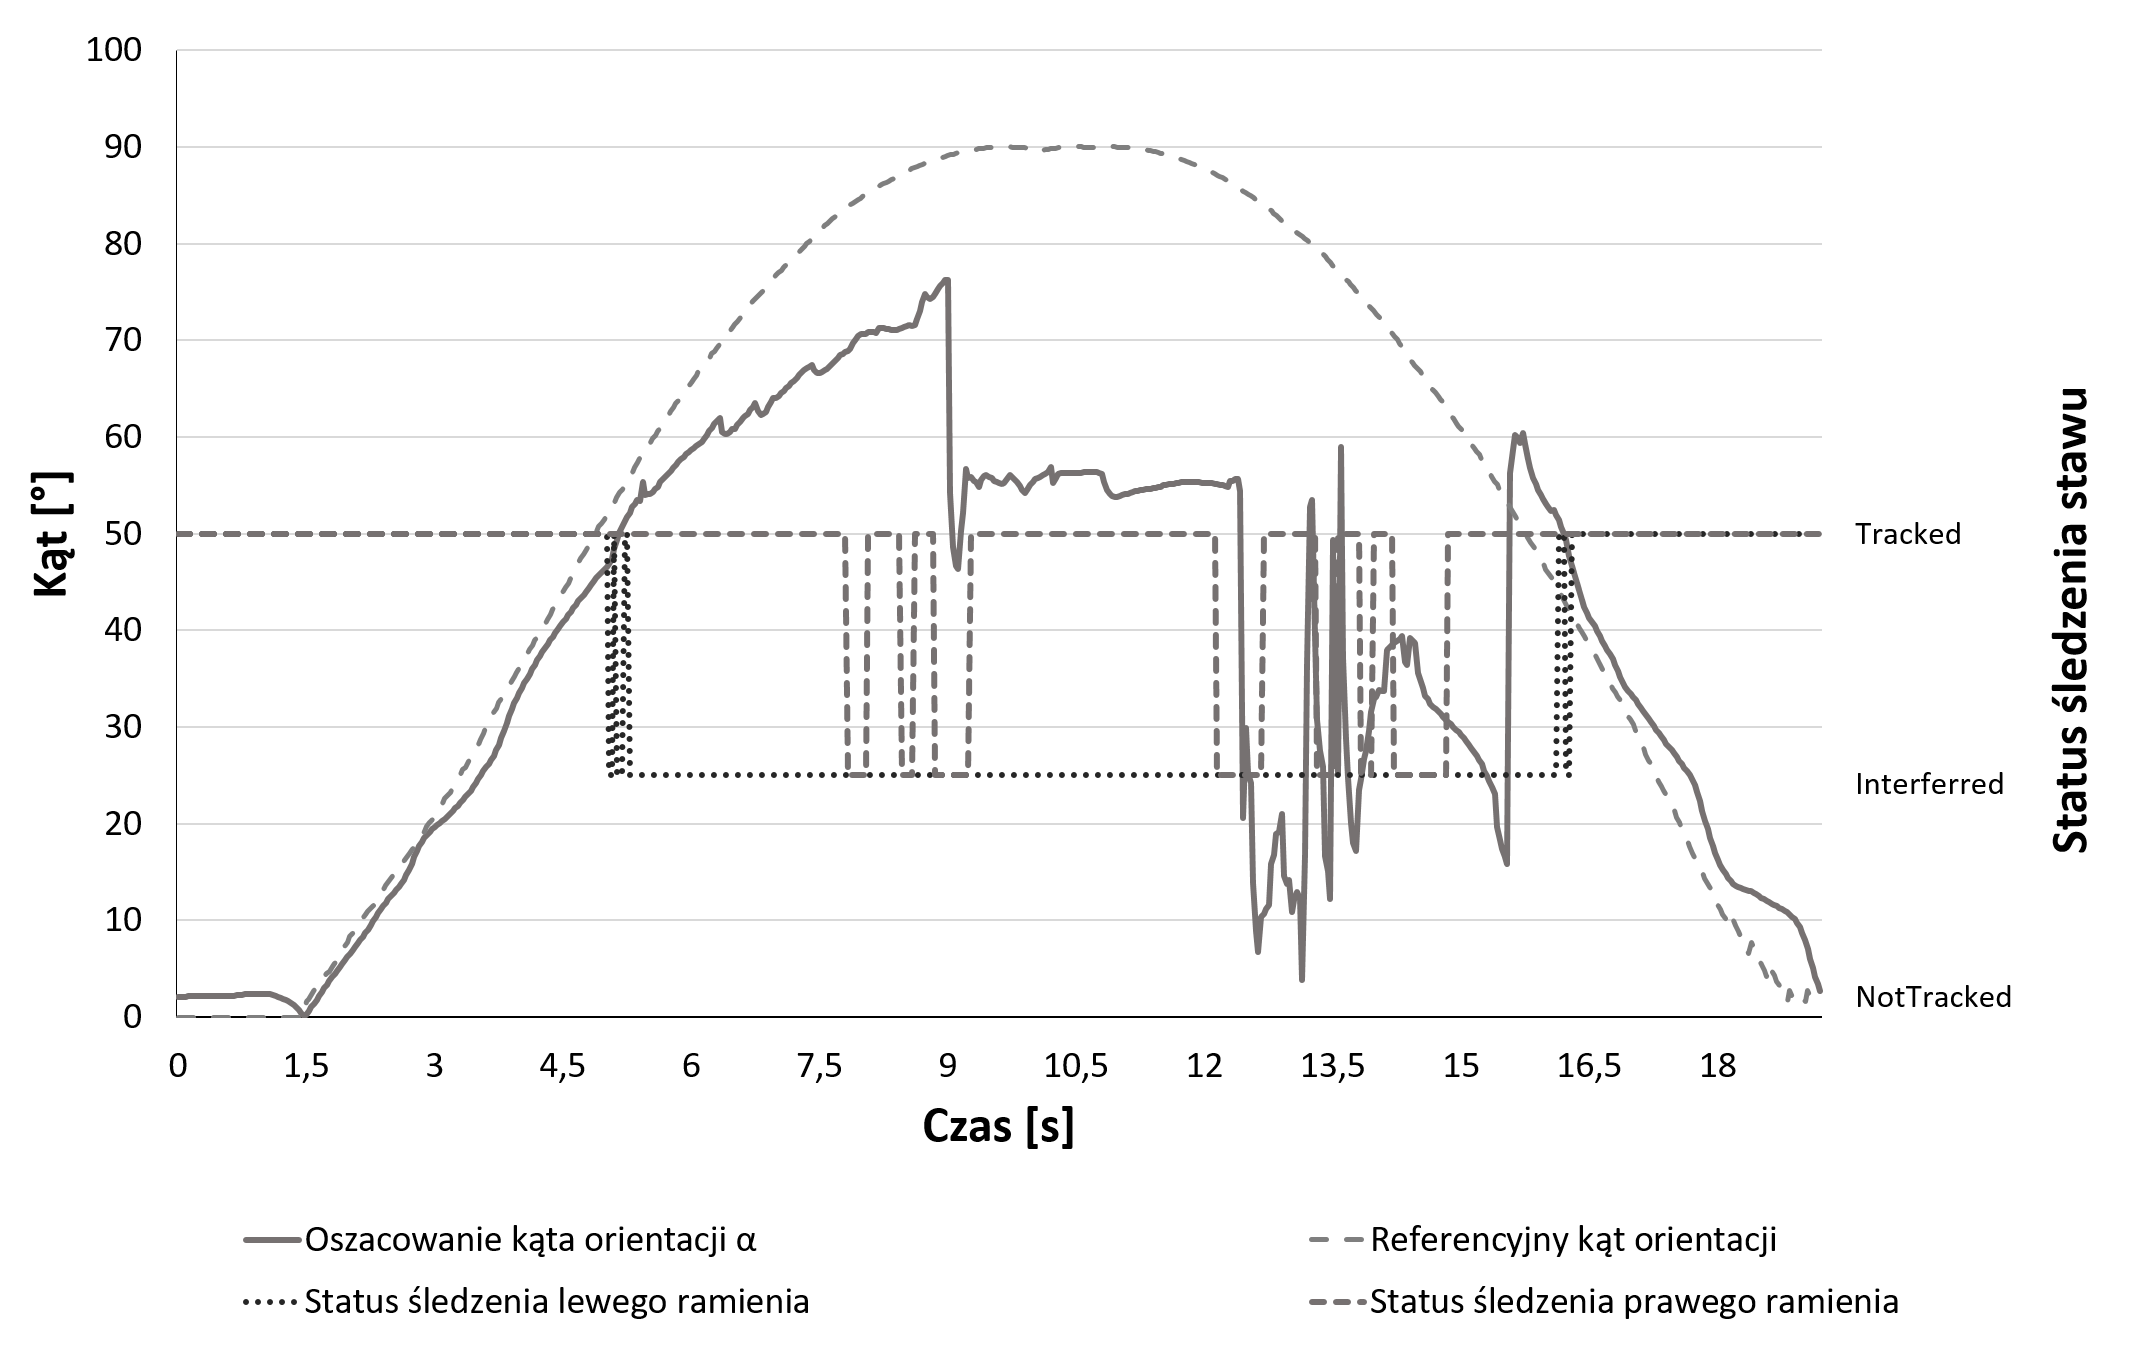
\includegraphics[scale=0.8]{images/kinectRotation.png}}
		\subfigure[Kąt w~łokciu prawej ręki podczas obrotu ciała \emph{(T-pose)} względem kontrolera]{\label{fig:characteristics:kinect:kinectRightHandElbowAngle}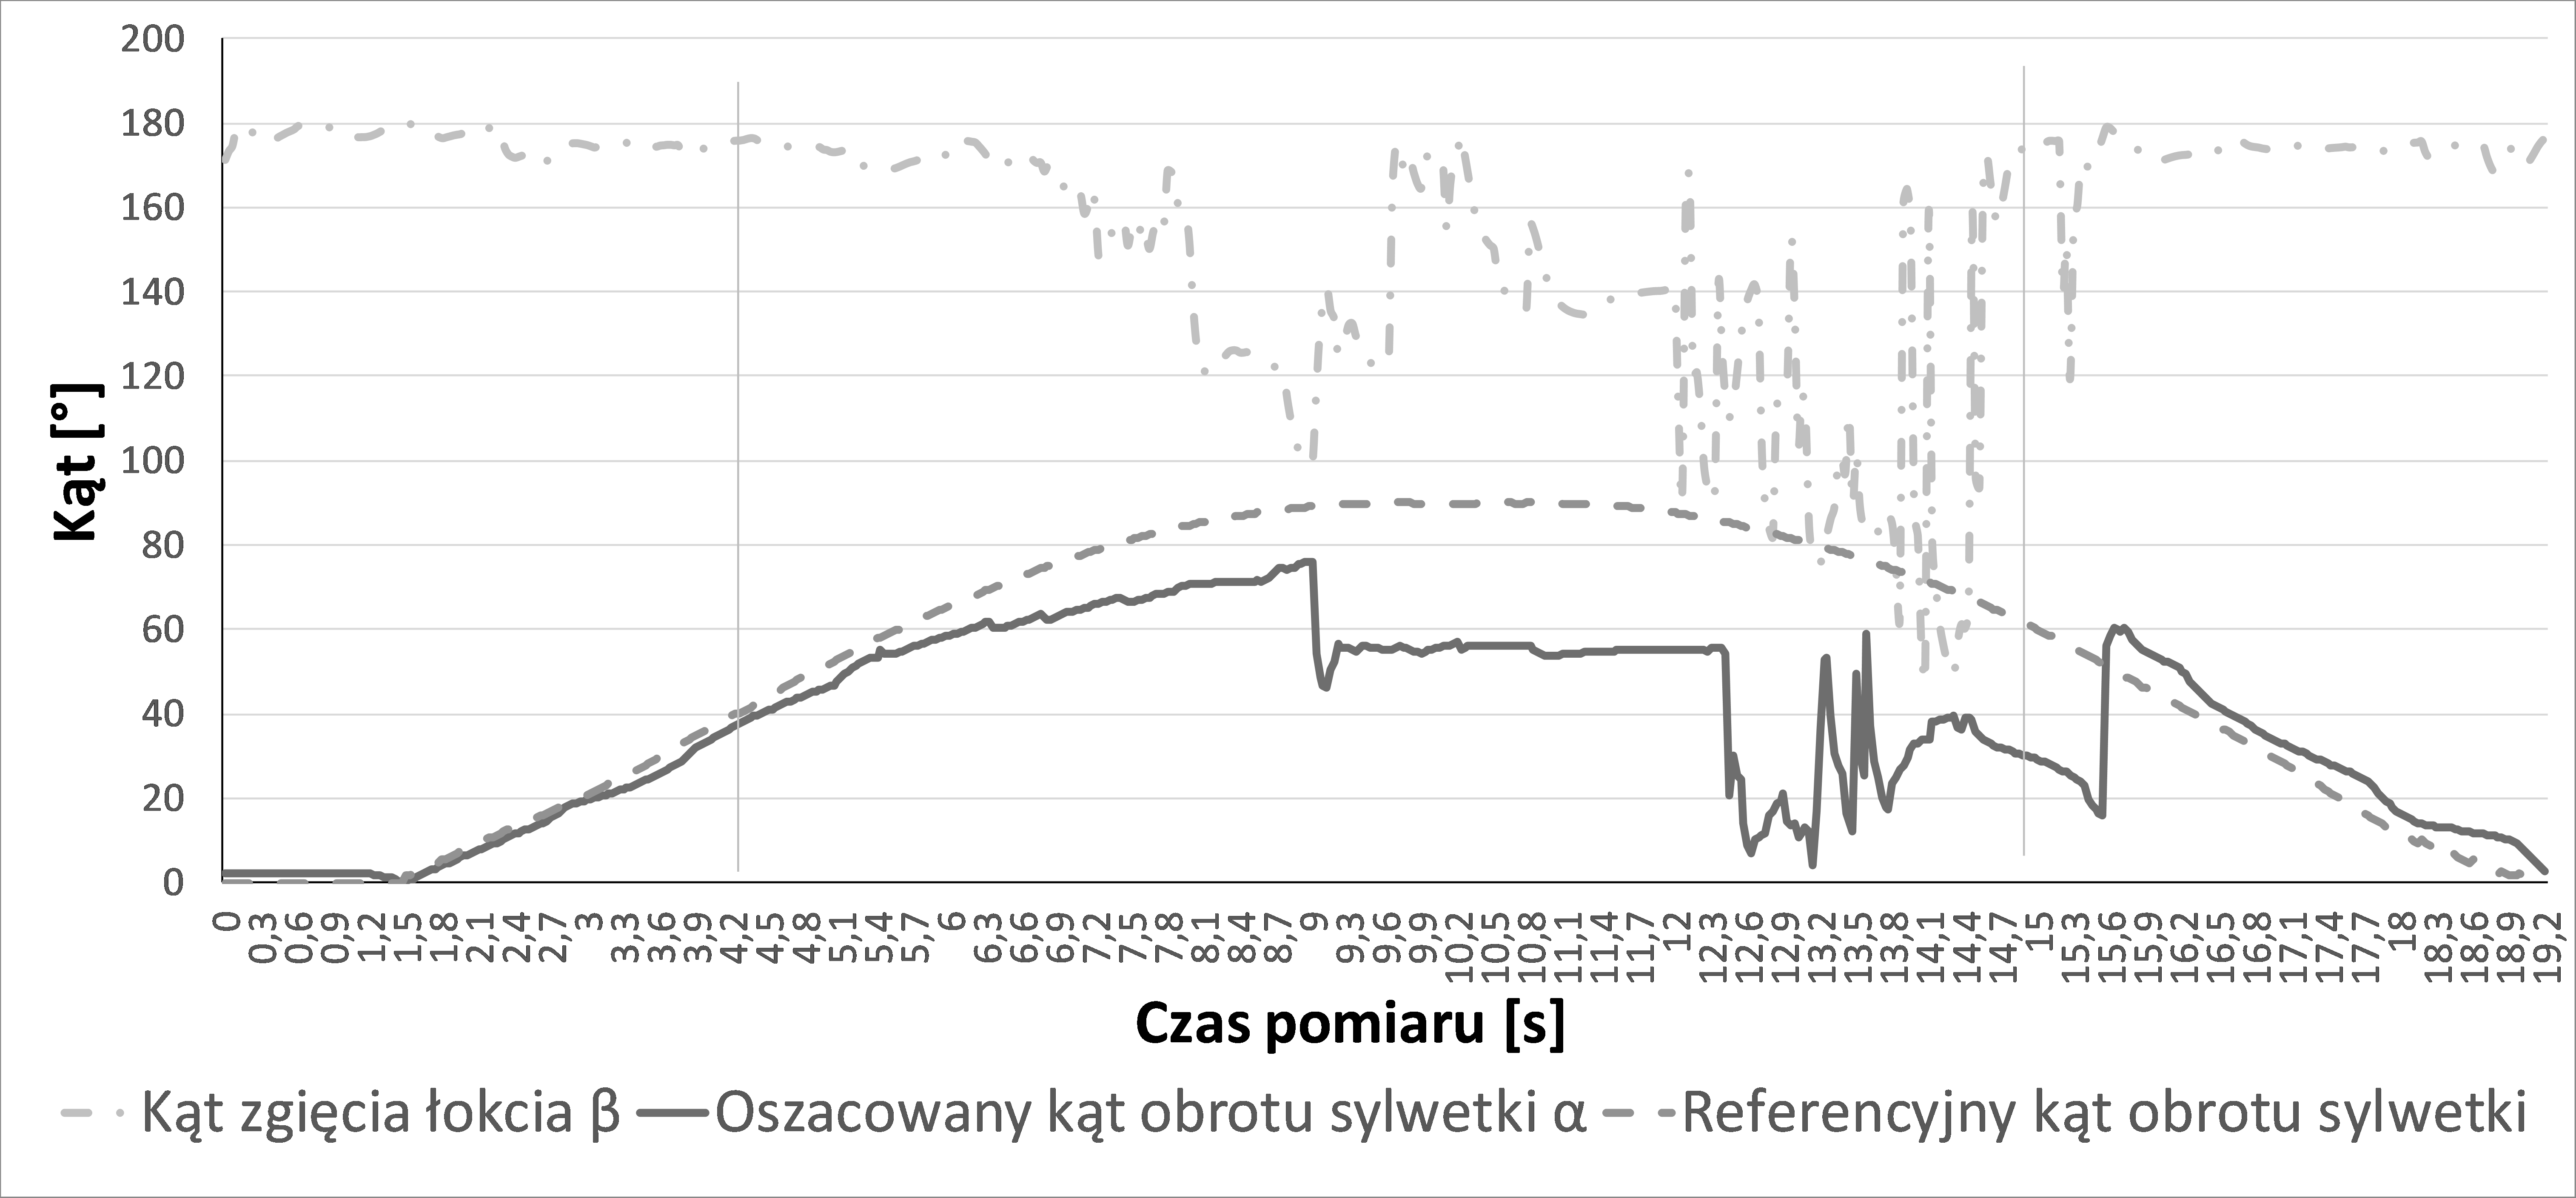
\includegraphics[scale=0.8]{images/kinectRightHandElbowAngle.png}} 
	\end{center}
										
	\caption{Pomiary zależne od kąta obrotu względem Kinecta [źródło własne]}
\end{figure}
		
\subsubsection*{Szacowanie odległości pomiędzy kontrolerem Kinect, a~śledzoną postacią}\label{sssection:distanceEstimation}
Kolejną istotną cechą kontrolera Kinect jest zmieniająca się dokładność szacowania głębi w~zależności od odległości w~jakiej znajduje się śledzona postać. Specyfikacja urządzenia nie zawiera informacji o~niejednorodności dokładności pomiaru, a~jedynie określa zakres w~jakim działa urządzenie. W~trakcie prowadzonych własnych badań nad charakterystyką kontrolera Kinect zaobserwowano zmianę dokładności szacowania głębi wraz z~oddalaniem się użytkownika od urządzenia. Eksperyment, dzięki któremu udało się zaobserwować omawianą zmianę dokładności szacowania odległości, polegał na płynnym oddalaniu się od kontrolera Kinect rejestrując uzyskany dzięki niemu pomiar odległości stawu barkowego oraz równoczesny pomiar tej samej odległości za pomocą systemu śledzenia Vicon. Wykres \ref{fig:characteristics:kinect:distanceAccuracy} przedstawia różnicę pomiędzy pomiarami uzyskanymi za pomocą kontrolera Kinect oraz tymi z~systemu Vicon. Pomiary z~systemu Vicon posłużyły jako dane referencyjne odpowiadające rzeczywistej odległości pomiędzy postacią a~kontrolerem Kinect oraz zostały wykorzystane jako dane na osi rzędnych. Jak widać na wykresie \ref{fig:characteristics:kinect:distanceAccuracy} zmiana dokładności oszacowania odległości w~jakiej znajduje się śledzona osoba od kontrolera Kinect, nie jest funkcją prostoliniową i~wraz z~oddalaniem się postaci od urządzenia pomiarowego zmienia się od niedoszacowania do przeszacowania wartości. Funkcja reprezentująca przybliżony model dokładności oszacowania odległości przez kontroler Kinect ma postać wielomianu 3-ego rzędu ($y = a_0 + a_1x + a_2x^2 + a_3x^3$). Wzór \eqref{eq:characteristics:kinect:distanceAccuracyPoly} przedstawia równanie pozwalające wyznaczyć współczynniki $a_0 ,a_1, a_2, a_3$ szukanego wielomianu. Macierze $X$ i~$Y$ wykorzystane we wzorze \eqref{eq:characteristics:kinect:distanceAccuracyPoly} zawierają odpowiednio argumenty i~wartości dla tych argumentów, na podstawie których możliwe będzie wyznaczenie współczynników wielomianu zawartych w~macierzy $A$. W~przypadku omawianego eksperymentu argumentami są wybrane odległości od Kinecta w~jakich znajdowała się śledzona postać, natomiast wartościami są różnice pomiędzy oszacowaniem Kinecta a~odległością uzyskaną dzięki pomiarom systemu Vicon we wspomnianych punktach (argumentach).
		
\begin{equation}
	\begin{split}
		X = 	\begin{bmatrix}
		x_1^0&x_1^1&x_1^2&x_1^3\\
		x_2^0&x_2^1&x_2^2&x_2^3\\
		x_3^0&x_3^1&x_3^2&x_3^3\\
		\dots\\
		x_n^0&x_n^1&x_n^2&x_n^3
		\end{bmatrix} ,
		A &= 	\begin{bmatrix}
		a_0\\a_1\\a_2\\a_3
		\end{bmatrix} ,
		Y = 
		\begin{bmatrix}
			y_0 \\y_1\\y_2\\\dots\\y_n
		\end{bmatrix} \\
		& \\
		X^TXA &= X^TY
	\end{split}
	\label{eq:characteristics:kinect:distanceAccuracyPoly}
\end{equation}
gdzie:
\begin{conditions}
	n			& liczba uzyskanych próbek pomiarowych,																\\
	X			& macierz zawierająca argumenty,																\\
	A			& macierz szukanych współczynników funkcji,																\\
	Y			& macierz wartości uzyskanych w~punktach pomiarowych.																\\
\end{conditions}
		
		
Na podstawie pomiarów uzyskanych w~trakcie eksperymentu opisanego powyżej, macierz współczynników została wyznaczona jak we wzorze \eqref{eq:characteristics:kinect:distanceAccuracyCoef}
\begin{equation}
	\label{eq:characteristics:kinect:distanceAccuracyCoef}
	\begin{bmatrix}
		a_0 \\a_1\\a_2\\a_3
	\end{bmatrix} = 
	\begin{bmatrix}
		- 0.25 \\  0.27 \\- 0.11\\0.02		
	\end{bmatrix}	
\end{equation}
		
\pgfplotsset{width=12cm,compat=1.8}
		
\begin{figure}
	\centering
	\begin{tikzpicture}
		\begin{axis}[
				xlabel={Odległość [m]},
				ylabel={Dokładność [m]},
				xmin=0, xmax=4,
				ymin=-0.2, ymax=0.3,
				xtick={0,0.5,1,1.5,2,2.5,3,3.5},
				ytick={-0.15,-0.1,-0.5,0,0.5,0.1,0.15,0.2,0.25},
				ymajorgrids=true,
				grid style=dashed,
			]
																							
			\addplot+[
				only marks,
				scatter,
				color=blue,
				mark=square,
			]
			coordinates {
				(0.85,-0.10)(1.00,-0.07)(1.20,-0.06)(1.40,-0.04)(1.60,-0.03)(1.80,-0.02)(1.96, 0.00)(2.08, 0.00)(2.20, 0.00)(2.32, 0.00)(2.50, 0.02)(2.70, 0.04)(2.90, 0.06)(3.10, 0.07)(3.35, 0.12)
			};
																							
			\addplot [
				dashed,
				domain=0.5:3.8, 
				samples=100, 
				color=blue,
			]
			{0.0194*x^3 - 0.1125*x^2 + 0.2672*x - 0.2472};
			\legend{$y = 0.02x^3 - 0.11x^2 + 0.27x - 0.25$}
		\end{axis}
	\end{tikzpicture}	
									
	\caption{Przybliżenie dokładności pomiaru głębi względem odległości śledzonej postaci od kontrolera Kinect [żródło własne].}
	\label{fig:characteristics:kinect:distanceAccuracy}
\end{figure}
		
Należy zauważyć, że zaprezentowana na wykresie \ref{fig:characteristics:kinect:distanceAccuracy} charakterystyka oszacowania odległości pomiędzy kontrolerem Kinect a~użytkownikiem dotyczy obszaru roboczego tego kontrolera (rys. \ref{fig:characteristics:kinect:range}). W~związku z~tym dokładność oszacowania pozycji poszczególnych stawów w~modelu szkieletowym użytkownika jest uzależniona od tego gdzie on się znajduje i~należy to uwzględnić w~prowadzonych obliczeniach aby wykazane niedokładności skorygować.
%([Fixed] trochę to poprzednie zdanie jakieś zapętlone)
Jest to o~tyle istotne, że na podstawie uzyskanych wyników, przestrzeń, w~której szacowanie odległości pomiędzy użytkownikiem a~Kinectem jest zbliżone do faktycznej odległości, wynosi jedynie $0.3m$ pomiędzy $2m$, a~$2.3m$ od kamery.  


		
\subsection{Urządzenia inercyjne}\label{sec:characteristics:imu}
		
Urządzenia inercyjne są czujnikami, których działanie opiera się na obserwacji i~mierzeniu wielkości fizycznych, jakie działają na te czujniki w~trakcie ruchu oraz w~spoczynku. Wyróżniamy dwa podstawowe czujniki inercyjne: akcelerometr mierzący przyspieszenia liniowe oraz żyroskop mierzący prędkości kątowe. Choć urządzenia te są znane i~stosowane od dawna, dopiero z~chwilą ich implementacji w~formie mikroukładów elektromechanicznych (MEMS -- \emph{microelectromechanical systems}) stały się one powszechnie dostępne i~stosowane np. w~telefonach, czy systemach nawigacji wewnątrz budynków (INS -- \emph{indoor navigation systems}). W~badaniach przedstawionych w~niniejszej pracy, wykorzystany został układ o~symbolu MPU-6050 firmy InvenSense integrujący oba te czujniki (tabela \ref{tab:characteristics:mpu:spec} zawiera podstawowe parametry pracy tego układu). Układ ten oprócz wcześniej wspomnianych czujników posiada wbudowany termometr oraz procesor ruchu pozwalający na przetworzenie danych pomiarowych i~udostępnienie ich w~postaci kwaternionu reprezentującego orientację układu w~przestrzeni. Algorytm wyznaczania orientacji układu zaimplementowany w~tym procesorze nie został jednak opublikowany w~żadnej dokumentacji, w~związku z~czym funkcjonalność ta nie była wykorzystywana w~badaniach.
		
\begin{table}[!htp]
	\caption{Zestawienie podstawowych parametrów pracy układu MPU-6050\cite{ivenSense:MPU6050}}
	\label{tab:characteristics:mpu:spec}
	\noindent
	\small
	\centering
	\begin{tabular}{|p{5cm}|p{8cm}|}
		\hline 
		Osie pomiaru:                             & X, Y, Z \newline (układ współrzędnych widoczny na rys. \ref{fig:characteristics:imu:space})               \\
		\hline
		Interfejs komunikacyjny:                  & I2C (TWI) - 400 kHz                                                                                           \\
		\hline
		Rozdzielczość danych:                   & 16-bitów dla każdej osi                                                                                     \\
		\hline
		Zakres pomiarowy  \newline akcelerometru: & programowalny: \newline $\pm2g$, \textbf{$\pm4g$}, $\pm8g$, $\pm16g$                                          \\
		\hline
		Zakres pomiarowy żyroskopu:              & programowalny: \newline $\pm250\degree/s$, \textbf{$\pm500\degree/s$}, $\pm1000\degree/s$, $\pm2000\degree/s$ \\
		\hline
	\end{tabular} 	
\end{table} 
		
We wszystkich badaniach w~niniejszej pracy wykorzystujących czujniki inercyjne, są one skonfigurowane do pracy w~zakresie  $\pm4g$ dla akcelerometru oraz $\pm500\degree/s$dla żyroskopu. Zakresy te zostały wybrane na podstawie specyfikacji komercyjnie dostępnego urządzenia pozwalającego na śledzenie ruchu -- Nintendo WiiRemote.
		
\begin{figure}[!htp]
	\centering 
	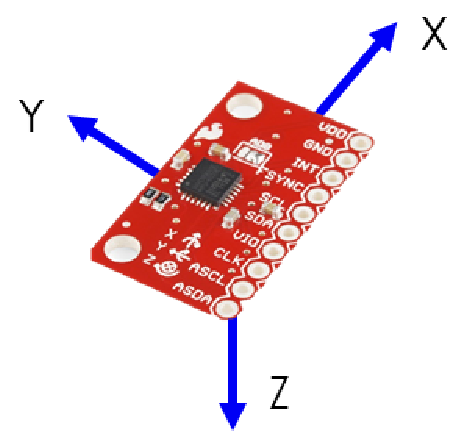
\includegraphics[width=0.35\textwidth]{images/imuCoordinationSpace.eps}	
	\caption{Układ współrzędnych wykorzystywany w~czujnikach MPU--6050}
	\label{fig:characteristics:imu:space}
\end{figure}
		
		
\subsubsection*{Akcelerometr}
Akcelerometr mierzy siłę działającą na niego w~dowolnym z~trzech kierunków, wyrażoną w~odniesieniu do siły grawitacji w~jednostkach ''g''. Pozwala to na szacunkowe określenie z~jakim przyspieszeniem wzdłuż każdej osi porusza się dany czujnik 
%([Fixed] obiekt czy czujnik?) 
($1g =9.80665^m/_{s^2}$). Ze względu na to, że siła grawitacji działa na wszystkie obiekty nieustannie, akcelerometr leżący horyzontalnie na płaskiej powierzchni i~nie poruszający się, będzie wskazywał wartość $1g$ wzdłuż osi równoległej do wektora grawitacji i~$0g$ w~pozostałych dwóch osiach. Pomijając wpływ szumów na odczyty pomiarów z~akcelerometru, jeśli dla nieporuszajacego się czujnika wartości pomiaru będą inne niż podane powyżej, oznacza to, że czujnik jednak nie leży w~pozycji horyzontalnej. Pomiar wynoszący $0g$ we wszystkich trzech osiach oznacza, że dany obiekt spada swobodnie w~orientacji idealnie horyzontalnej.\\
		
\begin{figure}[!htp]
	\subfigure[Struktura wewnętrzna \cite{memsAccStructure2016}]{
		\includegraphics[width=0.49\textwidth]{images/memsAccelerometerStructure.png}
		\label{fig:characteristics:imu:acc:memsA}}
	\subfigure[Wizualizacja budowy \cite{memsAccIdea2016}]{
		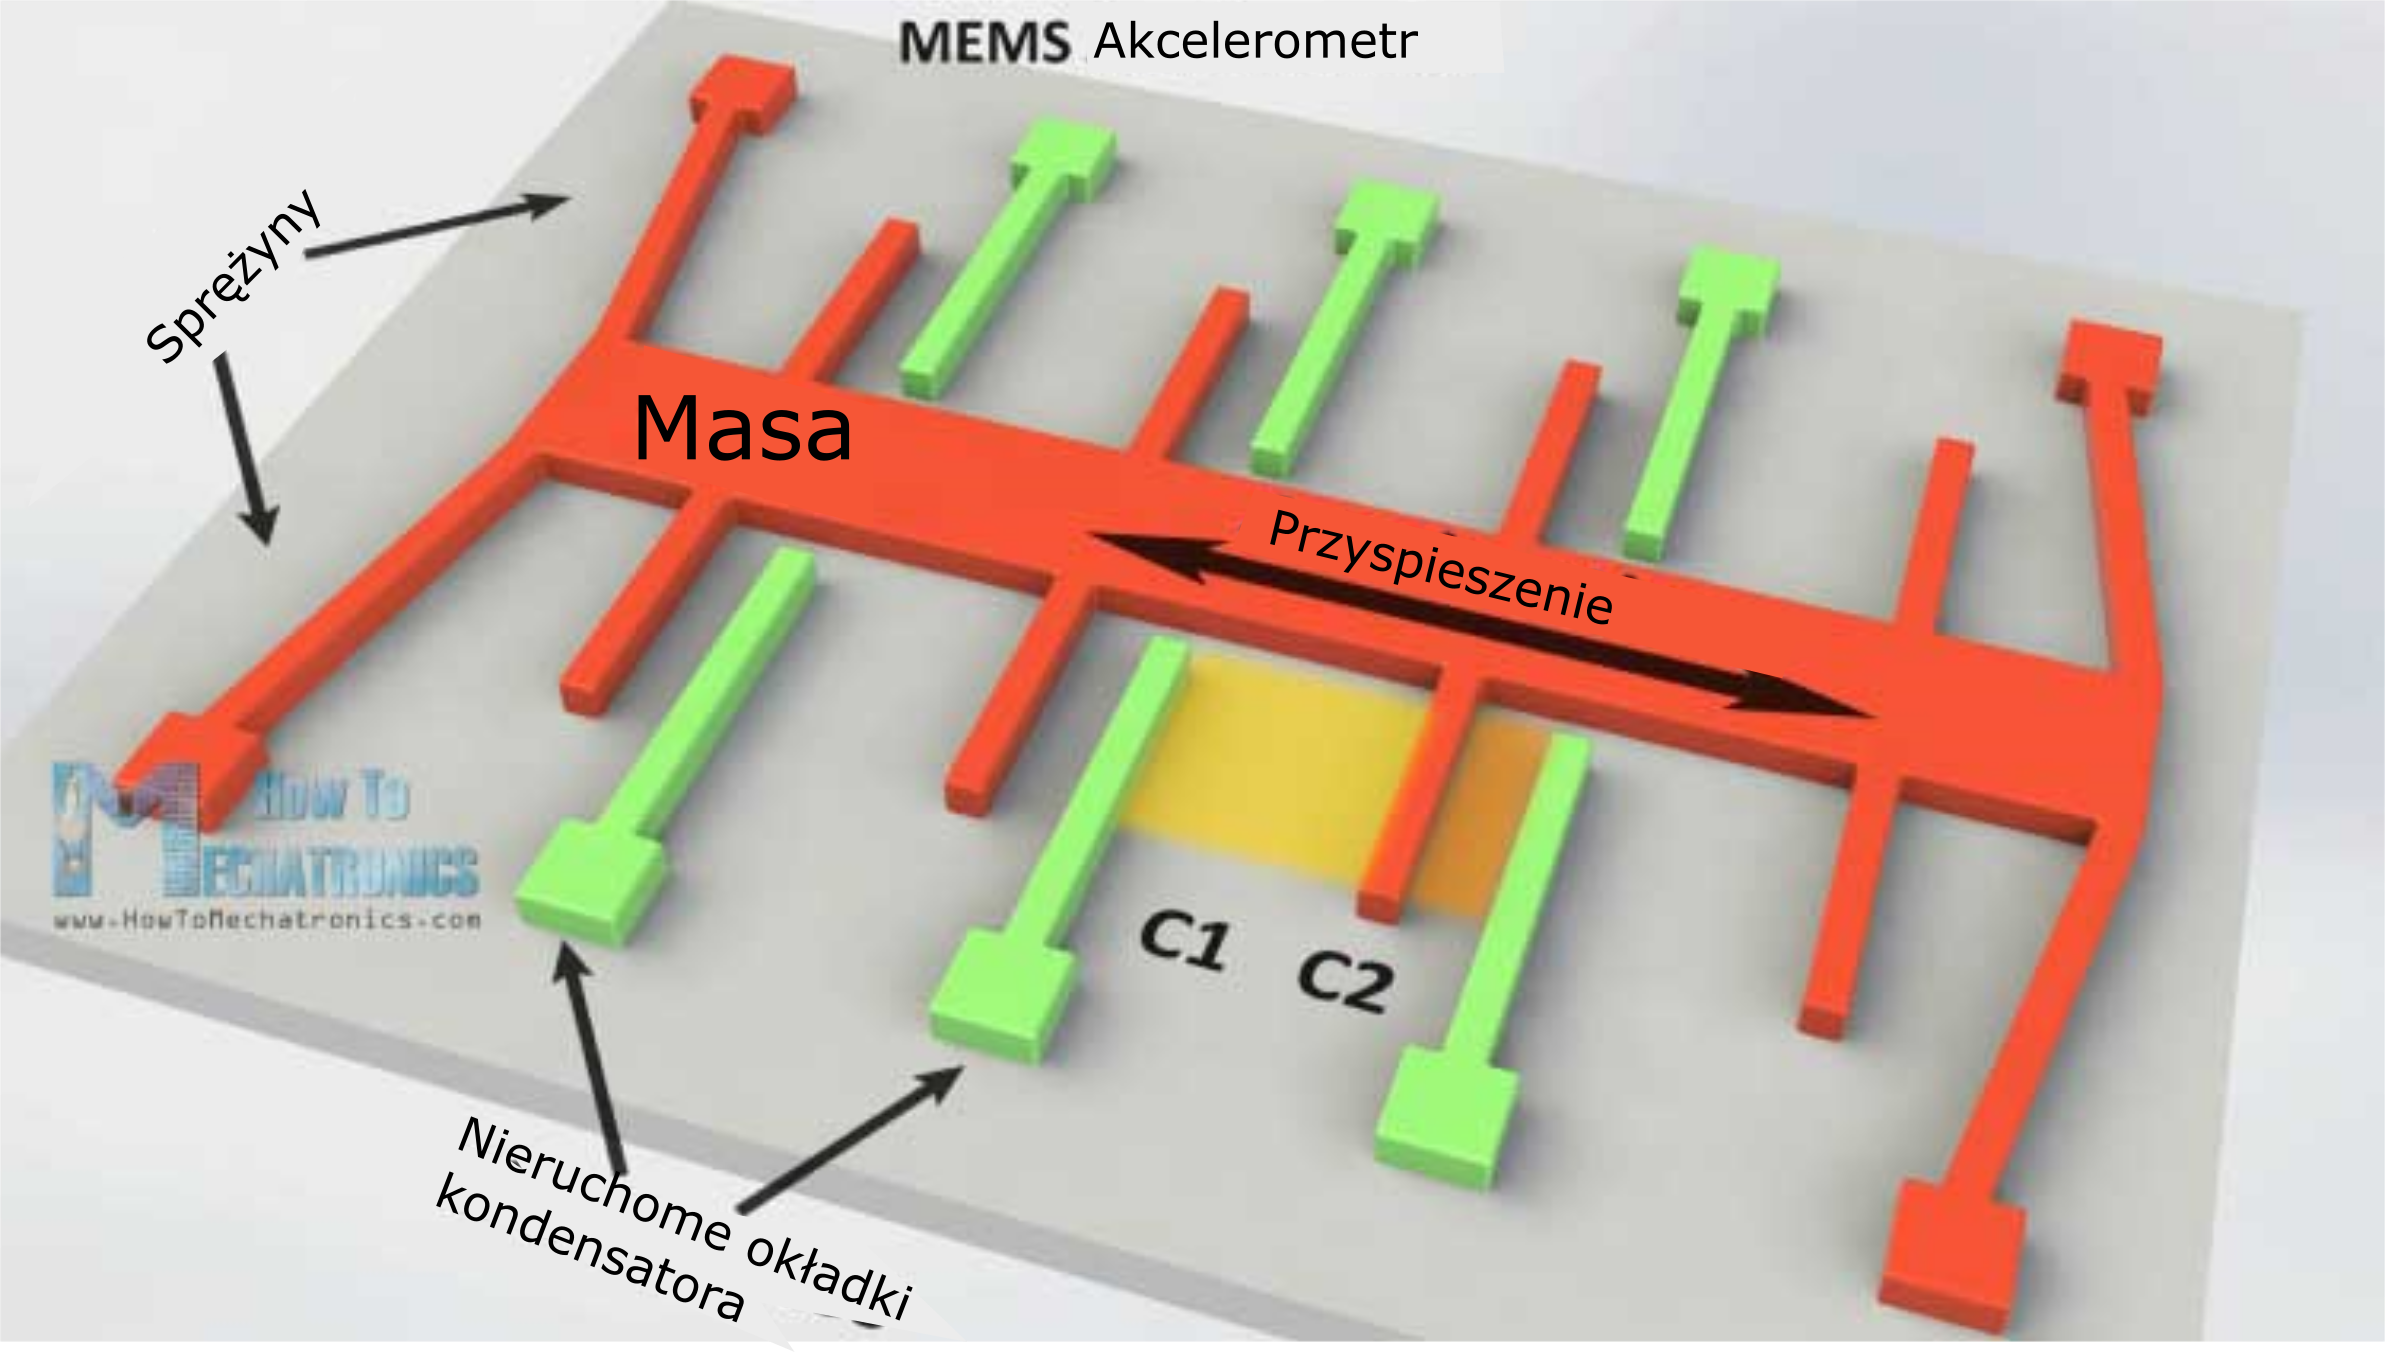
\includegraphics[width=0.49\textwidth]{images/memsAccelerometerIdea.png}
		\label{fig:characteristics:imu:acc:memsB}}
									
	\caption{Struktura wewnętrzna akcelerometru w~technologii MEMS}
	\label{fig:characteristics:imu:acc:mems}
\end{figure}
		
Zastosowany w~tym układzie akcelerometr jest czujnikiem typu pojemnościowego. Oznacza to, że jego wewnętrzna struktura opiera się na układzie ruchomych półprzewodnikowych belek ułożonych pomiędzy analogicznymi, nieruchomymi belkami, które tym samym tworzą układ kondensatorów (rys. \ref{fig:characteristics:imu:acc:mems}). Pomiędzy dwiema sąsiednimi nieruchomymi belkami znajduje się dokłądnie jedna belka ruchoma tworząc w~ten sposób parę dwóch kondensatorów o~zmiennych pojemnościach $C_1$ i~$C_2$. Siła działająca na czujnik powoduje przesunięcie się ruchomej belki w~kierunku przyłożonej siły o~dystans $d$. Przyjmując dystans pomiędzy nieruchomymi belkami a~belką ruchomą w~czasie spoczynku jako $d_0$ to przy powierzchni belek oznaczonej jako $s$ i~stałej dielektrycznej materiału z~którego wykonane są belki $\epsilon$, pojemności $C_1$ i~$C_2$ określone są wzorem \eqref{eq:characteristics:imu:acc:capacitor}.
	
\begin{subequations}
	\begin{align}
		C_1 = \frac{\epsilon s}{d_0 + d}             \\ 
		C_2 = \frac{\epsilon s}{d_0 - d}             
		\label{eq:characteristics:imu:acc:capacitor} 
	\end{align}
\end{subequations}
	
Następnie, na podstawie wartości $C_1$ i~$C_2$ i~wartości napięcia elektrycznego jaki zasila układ akcelerometru, możliwe jest wynaczenie wartości napięcia wypływającego z~takiej pary kondensatorów $V_C$ przy podanym napięciu wejściowym $V_0$ za pomocą wzoru \eqref{eq:characteristics:imu:capacityToVoltage}.

\begin{equation}
	V_C = V_0 \frac{C_2-C_1}{C_2+C_1} = V_0\frac{d}{d_0}
	\label{eq:characteristics:imu:capacityToVoltage}
\end{equation}
	
Ponieważ wartość napięcia $V_C$ jest zależna od przemieszczenia wartości $d$ ruchomej belki w~układzie dwóch kondesatorów, wartość ta odzwierciedla siłę jaka działa na dany czujnik. Bezpośredni odczyt wartości $V_C$ musi być jednak poddany dodatkowemu przetwarzaniu w~celu określenia kierunku w~jakim zadziałała siła. Kierunek działania siły na czujnik, odzwierciedlony jest w~postaci znaku $+$ albo $-$ przy wartości $V_C$. Następnie możliwe jest wyznaczenie wartości przyspieszenia $a$ działającego na dany czujnik. W~tym celu należy wykorzystać fakt, że siła sprężystości $F_s$ dla małych odkształceń, na podstawie prawa Hooke\'a, jest wprost proporcjonalna do odkształcenia sprężyny (w tym wypadku do przemieszczenia ruchomej belki $d$). Oznaczając przez $f_s$ współczynnik sprężystości charakterystyczny dla materiału z~którego zbudowana jest dana sprężyna, siłę sprężystości można zdefiniować wzorem \eqref{eq:characteristics:imu:springForce}

\begin{equation}
	F_s = f_s d
	\label{eq:characteristics:imu:springForce}
\end{equation}	
	
Wykorzystując drugie prawo Newtona możemy przedstawić związek pomiędzy siłą działającą na ciało, jego masą $m$ oraz jego przyspieszeniem $a$. Na tej podstawie wzór \eqref{eq:characteristics:imu:springForce} można przekształcić do postaci określonej wzorem \eqref{eq:characteristics:imu:springForceNewton}

\begin{equation}
	F_s = ma = f_s d
	\label{eq:characteristics:imu:springForceNewton}
\end{equation}	

Następnie łącząc ze sobą wzory \eqref{eq:characteristics:imu:capacityToVoltage} oraz \eqref{eq:characteristics:imu:springForceNewton} możemy wyznaczyć wartość przyspieszenia jak we wzorze \eqref{eq:characteristics:imu:acceleration}

\begin{equation}
	ma = f_s d \Rightarrow a~= \frac{f_s}{m} d = \frac{f_s}{m} \frac{d_0 V_C}{V_0}
	\label{eq:characteristics:imu:acceleration}
\end{equation}

Szczegółowy opis budowy i~działania akcelerometrów zbudowanych w~architekturze MEMS można znaleźć w~pracy Mateja Andrejasica z~Uniwersytetu w~Lubljanie \cite{Andrejasic2008}.

\subsubsection*{Żyroskop}
Budowa wykorzystanego żyroskopu, podobnie jak akcelerometru, opiera się na układzie kondensatorów o~zmiennej pojemności, jednak w~tym przypadku są one dodatkowo wprawione w~drgania. Działanie takiego żyroskopu opiera się na efekcie Coriolisa \cite{memsAccIdea2016}. Budowę i~uproszczony sposób działania czujnika przedstawia rysunek \ref{fig:characteristics:imu:gyro:mems}. Wykorzystane urządzenie mierzy prędkość kątową wokół 3 osi wyrażoną w~stopniach na sekundę ($^\degree/_s$), odpowiadającą konwencji nazewniczej związanej z~reprezentacją obrotów w~postaci kątów Eulera (rozdział \ref{chap:orientstionRep}). 
		
\begin{figure}[!htp]
	\subfigure[Struktura wewnętrzna \cite{memsGyroStructure2016}]{
		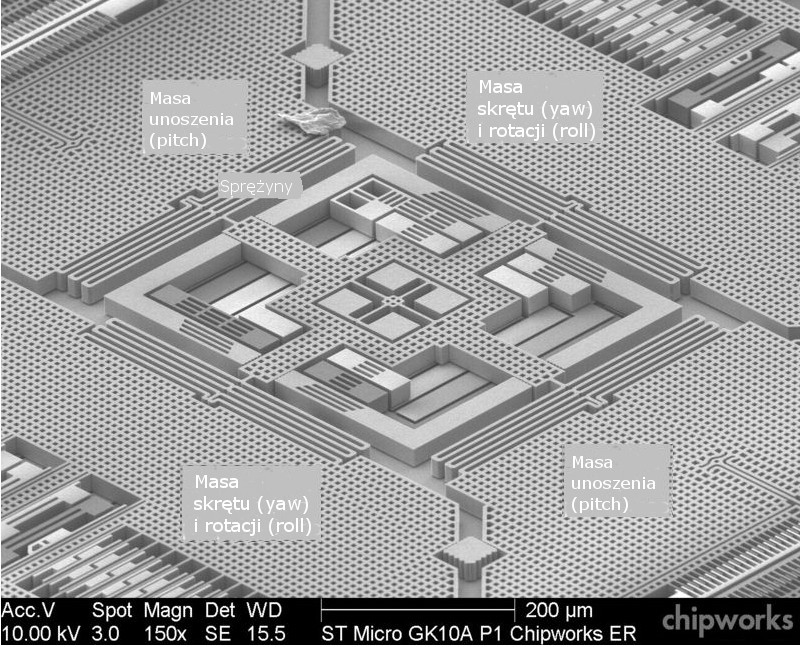
\includegraphics[width=0.49\textwidth]{images/memsGyroscopeStructure.jpg}}
	\subfigure[Wizualizacja budowy \cite{memsAccIdea2016}]{
		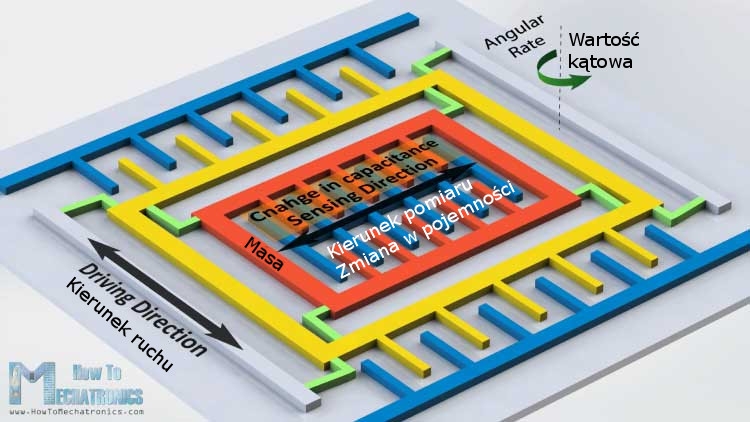
\includegraphics[width=0.49\textwidth]{images/memsGyroscopeIdea.jpg}}
										
	\caption{Struktura wewnętrzna żyroskopu w~technologii MEMS}
	\label{fig:characteristics:imu:gyro:mems}
\end{figure}
		
\subsection{Ograniczenia w~działaniu czujników inercyjnych}
Ograniczenia w~działaniu obu czujników inercyjnych można rozdzielić na te dotyczące ogólnie urządzeń stworzonych w~architekturze MEMS, a~tym samym wynikające z~ich budowy i~właściwości fizycznych, oraz na te charakterystyczne dla poszczególnych rodzajów czujników związane z~ich działaniem np.: szum danych, czy wpływ temperatury urządzenia na uzyskiwane pomiary.
		
\paragraph*{Zaszumienie danych}
Pomiary dostarczane przez oba czujniki zawierają szum, który w~znaczący sposób wpływa na dalsze obliczenia. Do określenia charakteru zakłóceń pomiaru najczęściej wykorzystuje się wariancje oraz odchylenie Allana\cite{Allan1966}, która to metoda została przyjęta przez IEEE jako standardowa do określania szumu w~IMU \cite{IeeeAccSpec}. Z uzyskanych za pomocą tej metody wyników można odczytać, że dwoma typami szumów, które przeważają w~sygnalne uzyskanym z~żyroskopu i~akcelerometru są: błądzenie losowe związane z~mierzonymi wielkościami (ang. \emph{angular/velocity random walk}), a~także szum o~wysokiej częstotliwości oraz niestabilność błędu systematycznego (ang. \emph{bias instablity}) o~niskiej częstotliwości. Fakt występowania obu szumów w~czujnikach inercyjnych jest dodatkowo powiązany z~różnymi charakterystykami częstotliwościowymi właściwych sygnałów. Dla akcelerometru, mierzącego działające na niego siły w~odniesieniu do siły grawitacji, sygnał prawidłowy jest o~niskiej częstotliwości, więc szczególnego znaczenia nabiera zakłócenie i~zmienność wartości błędu systematycznego. Z kolei sygnał zarejestrowany przez żyroskop jest wysokoczęstotliwościowy, więc błądzenie losowe wpływa na uzyskane wyniki.
		
\paragraph*{Temperatura pracy}
Jednym z~czynników wpływających na jakość pomiarów uzyskiwanych za pomocą czujników tworzonych w~architekturze MEMS jest temperatura pracy tych urządzeń.
%Temperatura pracy urządzenia jest jednym z~tych czynników wpływających na jakość uzyskiwanych pomiarów, który jest charakterystyczny dla niemal wszystkich urządzeń tworzonych w~architekturze MEMS. 
%([Fixed] trochę to zdanie brzmi nie po polsku) 
Jej wpływ na uzyskiwane wyniki, jak w~swojej analizie wskazują Liu et al. \cite{Liu2007, Liu2015}, mają 3 czynniki: moduł Younga, deformacja materiału pod wpływem temperatury oraz naprężenia materiału. Każdy z~tych czynników wpływa na możliwości przepływu prądu w~omawianych układach, co bezpośrednio wpływa na jakość interpretacji zgromadzonych ładunków w~kondensatorach układów MEMS. Zgodnie ze specyfikacją układu MPU-6050, temperatura neutralna dla ich pracy to 25 $\degree C$, a~błąd związany z~temperaturą urządzenia zmienia się nieliniowo. Zmiana temperatury układów MEMS wynika z~temperatury otoczenia, w~której pracują oraz z~naturalnego wydzielania się ciepła podczas pracy. W~wyniku własnych eksperymentów udało się zaobserwować wpływ zmiany temperatury na uzyskane pomiary przyspieszenia ziemskiego w~zakresie temperatur 10-50 $\degree C$ (rys. \ref{fig:characteristics:imu:temp}). Ponieważ temperatura pracy urządzeń umieszczonych przy ciele stabilizuje się przy 32 $\degree C$, czynnik ten musi być wzięty pod uwagę i~skorygowany przed obliczeniami bazującymi na danych akcelerometru. Podobnej zależności nie zaobserwowano w~przypadku używanych żyroskopów. Prawdopodobną przyczyną jest fakt, że temperatura wpływa na sygnały o~niskiej częstotliwości, które są odfiltrowane w~trakcie odczytu pomiarów. Wynika to z~faktu, że prawidłowy sygnał, jaki rejestrowany jest przez żyroskop, powinien mieć wysoką częstotliwość, a~w~związku z~tym cały sygnał przetwarzany jest filtrem górnoprzepustowym. W~takim przypadku szum niskiej częstotliwości jest w~dużym stopniu usunięty z~uzyskiwanych pomiarów.
		
\begin{figure}
	\centering
	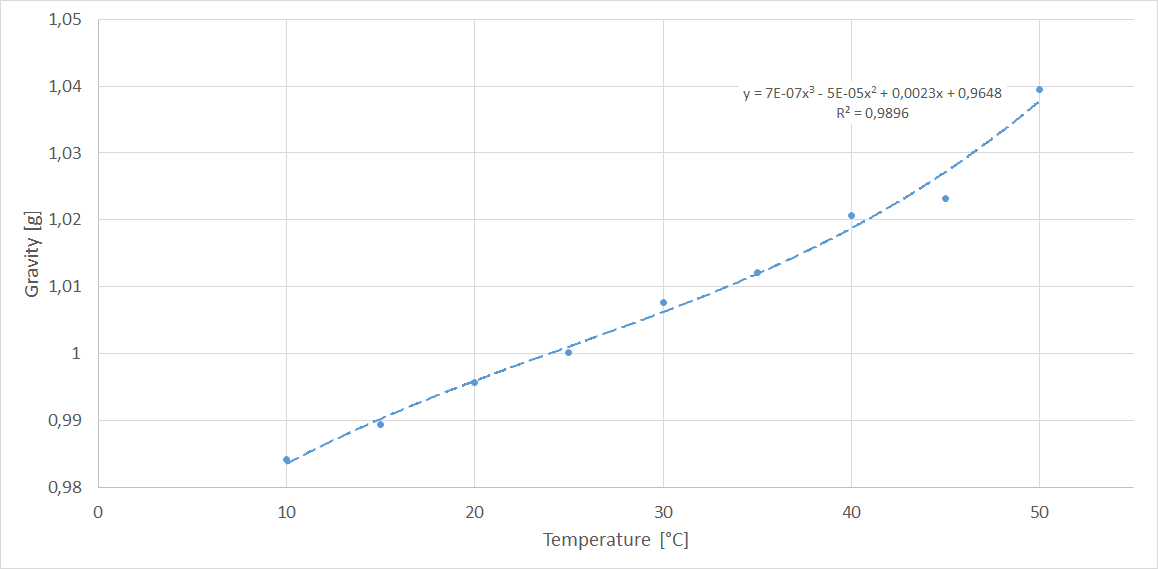
\includegraphics[width=0.8\textwidth]{images/temp.png}
	\caption{Pomiar przyspieszenia ziemskiego w~przedziale temperatur 10-50$\degree C$ [źródło własne]}
	\label{fig:characteristics:imu:temp}
\end{figure}
		
\paragraph*{Niepełna informacja o~obrotach}
Do precyzyjnego określenia orientacji, w~przestrzeni urządzenia pomiarowego złożonego z~czujników inercyjnych i~magnetycznych, nie powinno się bazować jedynie na pojedynczym czujniku (np. wyłącznie na żyroskopie), ale należy połączyć ze sobą sygnały (ang. \emph{data fusion}) z~kilku różnych czujników np: akcelerometru i~żyroskopu, czy żyroskopu i~magnetometru. Wynika to z~szumów jakie występują w~mierzonych sygnałach i~konieczności ich odfiltrowania. Ponieważ charakterystyki szumów i~sygnałów mierzonych przez każdy z~czujników różnią się od siebie, to właśnie zsynchronizowane łączenie danych daje rezultaty lepsze niż np. zastosowanie filtracji na pojedynczym sygnale. Jakość uzyskanych wyników takiego łączenia danych jest zależna od wybranej metody (rozdział \ref{chap:appx:filters}) oraz posiadanej wiedzy dotyczącej charakterystyk urządzeń. W~przypadku zastosowania pary akcelerometr -- żyroskop, pomimo tego, że każdy z~nich jest urządzeniem 3-osiowym, możliwe jest wyznaczenie orientacji jedynie względem 2 osi. Ograniczenie to wynika z~pomiarów, jakie można uzyskać z~akcelerometru. Aby móc połączyć ze sobą dane z~obu czujników, zarówno akcelerometr jak i~żyroskop muszą udostępnić dane dotyczące obrotów wokół tych samych osi. O ile żyroskop faktycznie dokonuje pomiaru prędkości kątowych wokół wszystkich 3 osi, o~tyle akcelerometr podaje informację o~tym jak czujnik jest obrócony tylko względem dwóch osi. Dla akcelerometru, obrót wokół osi działania siły grawitacji (obrót względem osi $Z$ na rys. \ref{fig:characteristics:imu:space}) jest niemierzalny, ponieważ obrót taki nie zmienia wartości z~jaką ta siła działa na czujnik w~danej chwili. Z tego zaś powodu, orientacja względem osi działania siły grawitacji nie jest wyznaczona drogą łączenia danych z~akcelerometru i~żyroskopu, a~jedynie może być wyznaczona na podstawie całkowania prędkości kątowej zmierzonej przez sam żyroskop, co jest obarczone znaczącymi błędami z~uwagi na zaszumienie danych. W~związku z~tym nie bierze się tej wartości pod uwagę w~obliczeniach i~przyjmuje się, że urządzenia oparte tylko na parze czujników inercyjnych określają orientację względem dwóch osi.\\
		
%([Fixed?] może jakieś zatem podsumowanie rozdziału?)(Czy ten tekst poniżej który przepisałeś może być podsumowaniem?)
\section{Podsumowanie}
Opisane w~niniejszym rozdziale urządzenia pomiarowe: kontroler Microsoft Kinect oraz czujniki inercyjne: akcelerometr i~żyroskop, są wykorzystywane do budowy dwóch różnych systemów śledzenia ruchu. Wykorzystując kontroler Microsoft Kinect można zbudować optyczny system śledzenia ruchu nie wykorzysujący markerów (roz. \ref{chap:mocaps:Kinect}), a~z kolei akcelerometry i~żyroskopy stanowią podstawę dla nieoptycznych inercyjnych systemów śledzenia ruchu (roz. \ref{chap:mocaps:IMU}). Opierając się na charakterystykach zarówno wspomnianych urządzeń pomiarowych jak i~cechach systemów śledzania ruchu na nich opartych, badacze zwrócili uwagę na możliwość tworzenia hybrydowych systemów śledzenia ruchu, które opierają się na kontrolerze Kinect, akcelerometrach oraz żyroskopach. Tworzenie takich hybrydowych systemów śledzenia ruchu możliwe jest dzięki temu, że urządzenia pomiarowe, które wykorzystują, mogą się wzajemnie uzupełniać w~działaniu.
		
% https://msdn.microsoft.com/en-us/library/jj131024.aspx
% https://msdn.microsoft.com/en-us/library/jj131429.aspx
% https://msdn.microsoft.com/en-us/library/hh973073.aspx
		
% http://users.dickinson.edu/~jmac/selected-talks/kinect.pdf
% https://orbi.ulg.ac.be/bitstream/2268/104993/1/Lejeune2011TheSecrets.pdf
% http://www.sci.utah.edu/~gerig/CS6320-S2013/Materials/CS6320-CV-S2012-StructuredLight.pdf
% http://home.agh.edu.pl/~hyla/Downloads/ASiUT/Cwiczenie_2/ASiUT_2.pdf
% http://www.eletel.p.lodz.pl/programy/sv/publikacje/pdf/12.pdf
		
		
		
% https://msdn.microsoft.com/en-us/library/jj131033.aspx
% https://www.ifixit.com/Teardown/Xbox+360+Kinect+Teardown/4066
% http://stackoverflow.com/questions/7696436/precision-of-the-kinect-depth-camera
% https://msdn.microsoft.com/en-us/library/hh855368
% https://azttm.wordpress.com/2011/04/03/kinect-pattern-uncovered/
% http://www.freepatentsonline.com/20100118123.pdf
% http://www.freepatentsonline.com/20100020078.pdf
		
%Opisane w~niniejszym rozdziale urządzenia pomiarowe: kontroler Microsoft Kinect oraz czujniki inercyjne akcelerometr i~żyroskop, są wykorzystywane do budowy dwóch różnych systemów śledzenia ruchu. Wykorzystując kontroler Microsoft Kinect można zbudować optyczny system śledzenia ruchu nie wykorzysujący markerów(roz. \ref{chap:mocaps:Kinect}), a~z kolei akcelerometry i~żyroskopy stanowią podstawę dla nieoptycznych inercyjnych systemów śledzenia ruchu (roz. \ref{chap:mocaps:IMU}). Opierając się na charakterystykach zarówno wspomnianych urządzeń pomiarowych jak i~cechach systemów śledzania ruchu na nich opartych, badacze zwrócili uwagę na możliwość tworzenia hybrydowych systemów śledzenia ruchu, które opierają się na kontrolerze Kinect, akcelerometrach oraz żyroskopach. Tworzenie takich hybrydowych systemów śledzenia ruchu możliwe jest dzięki temu, że urządzenia pomiarowe na których się opierają moga się wzajemnie uzupełniać w~działaniu.
		
		
		
\section{Systemy hybrydowe łączące optyczny system śledzenia ruchu bez markerów oraz inercyjny system śledzenia ruchu}
Poszukiwanie rozwiązań pozwalających na łączenie ze soba optycznych systemów śledzenia ruchu bez markerów oraz inercyjnych systemów śledzenia jest zagadnieniem stosunkowo często spotykanym w~literaturze. Wiele ośrodków badawczych na całym świecie prowadzi badania w~tym obszarze mające na celu zwiększenie dokładności pozycjonowania stawów i~śledzenia ich ruchu. Obecnie, dzięki powszechnej dostępności urządzeń pomiarowych takich jak kontroler Kinect oraz akcelerometry i~żyroskopy jak również dzięki badaniom związanym z~ich połączeniem w~jeden system, można budować hybrydowe systemy śledzenia ruchu o~wysokiej dokładności, które mogą być dostępne do użytku domowego. Otwiera to z~kolei wiele możliwości w~obszarze zastosowań takich systemów, jak chociażby zaawansowane systemy do telerehabilitacji, czy programy do precyzyjnych treningów sportowych. W~dalszej części pracy przedstawione zostaną te opracowania, które wykorzystują kamery RGB-D dostępne na rynku konsumenckim (w~szczególności kontroler Kinect) oraz urządzenia inercyjne lub magnetyczne. \\
W 2014 roku Destelle et al. \cite{Destelle2014} zaproponował połączenie ze sobą kontrolera Kinect oraz systemu inercyjnego, w~celu stworzenia kompletnego systemu śledząco--pozycjonującego, nie korzystającego z~sygnału GPS oraz zaawansowanych systemów LPM w~celu określenia położenia użytkownika na scenie. W~rozwiązaniu autorów Kinect został wykorzystany na dwa sposoby:
\begin{enumerate}
	\item jako system definiujący model szkieletowy,
	\item jako system odpowiedzialny za śledzenie położenia aktora na scenie.
\end{enumerate}
		
W omawianym rozwiązaniu autorzy zdecydowali się na wykorzystanie urzdzeń inercyjnych stworzonych przez firmę X-IO Technologies \cite{xIo}. Urządzenia inercyjne firmy X-IO Technologies to układy zbudowane na bazie czujników inercyjnych oraz czujników inercyjnych wspieranych przez czujnik magnetyczny. Łączenie danych z~tych czujników, mające na celu określić orientację przestrzenną urządzenia, stosuje autorską metodę założyciela tej firmy, nazwaną jego nazwiskiem -- metodę Madgwicka.\\
Aby uniknąć konieczności budowania modelu szkieletowego na podstawie własnych pomiarów, na potrzeby systemu inercyjnego, autorzy postanowili wykorzystać estymację szkieletu dokonywaną przez Kinecta. Aby uniknąć problemów związanych ze zmiennością szacowania długości poszczególnych kości, a~co za tym idzie zmiennością proporcji modelu szkieletowego, niezbędne pomiary pozwalające wyznaczyć model szkieletowy dokonywane są tylko raz w~czasie inicjalizacji systemu i~zostają przyjęte jako stałe na cały czas trwania śledzenia ruchu. W~trakcie śledzenia ruchu rolą urządzeń inercyjnych było określenie orientacji przestrzennej tych kości, do których owe urządzenia były przymocowane, a~rolą Kinecta było określenie położenia całego modelu postaci na scenie. Pozycjonowanie modelu na scenie zostało zrealizowane poprzez obserwowanie przez kontroler Kinect położenia pojedynczego punktu znajdującego się na korpusie obserwowanej postaci. Przemieszczenie tego pojedynczego punktu traktowane jest jako przemieszczenie całego wyznaczonego modelu szkieletowego. W~omawianym artykule Destelle wskazuje średniokwadratowy błąd wyznaczania kątów zgięcia kończyn w~stawach na $4\degree$ -- $14\degree$ w~zależności od stawu, wobec błędu średniokwadratowego w~przedziale $10\degree$ -- $30\degree$ dla tych samych stawów w~przypadku pomiaru wyłacznie za pomocą samego kontrolera Kinect. Warto jednak zauważyć, że w~przypadku pomiarów obarczonych największym błędem średniokwadratowym następowała czasowa utrata śledzenia poszczególnych stawów. Autor nie zamieścił natomiast żadnych danych pozwalających na oszacowanie dokładności wyznaczenia pozycji poszczególnych stawów. Łatwo można zauważyć, że system zaproponowany przez Destelle nie wykorzystuje w~pełni możliwości łączenia danych z~obu urządzeń, gdyż wykorzystywane są one w~odrębnych obszarach i~mają minimalny wpływ na siebie. Stąd, porównanie dokładności samego Kinecta z~dokładnością systemu hybrydowego w~zakresie mierzenia zgięcia kończyn w~stawach jest de facto porównaniem dokładności tego pierwszego z~urządzeniem Madgwicka. Z drugiej zaś strony, omawiany system dobrze pokazuje zasadność wykorzystania w~badaniach łatwo dostępnych i~tanich urządzeń inercyjnych, które pozwalają poprawić wyniki kontrolera Kinect.\\
		
Bo et al. \cite{Bo2011a} w~swoich badaniach w~2011 roku zaproponował metodę szacowania kąta stawu kolanowego wykorzystując układ czujników inercyjnych o~pięciu stopniach swobody (2 stopnie swobody dla żyroskopu i~3 stopnie swobody dla akcelerometru) oraz Kinecta. Metoda ma niejako 2 tryby działania: dla sytuacji kiedy dane z~Kinecta są dostępne i~wtedy kiedy ich brakuje. W~obu przypadkach to czujniki inercyjne są wykorzystywane do oszacowania kąta zgięcia kończyny w~obserwowanym stawie, przy czym wartości te obliczane są osobno dla żyroskopu ($\Theta_G$) i~akcelerometru ($\Theta_A$). Oszacowanie wartości kąta, wykorzystuje całkownie pomiarów żyroskopu ($\tilde{\omega}_y$) zgodnie ze wzorem \eqref{eq:literature:bo:gyro} oraz na obliczeniach trygonometrycznych bazujących na stosunku siły działającej na akcelerometr w~wybranej osi ($f_x , f_z$) do siły grawitacji $g$ wg wzoru \eqref{eq:literature:bo:acc}. Następnie wartości te są ze sobą łączone z~wykorzystaniem liniowego filtru Kalmana.
		
\begin{equation}
	\Theta_G = \int{\tilde{\omega}_y dt}
	\label{eq:literature:bo:gyro}
\end{equation}
		
\begin{equation}
	\Theta_A = \alpha \arccos{\frac{f_x}{\norm{g}}} + (1 - \alpha) \arcsin{\frac{f_z}{\norm{g}}}
	\label{eq:literature:bo:acc}
\end{equation}
		
W przypadku dostępności danych z~Kinecta, dodatkowym krokiem jest korekta pomiarów na podstawie danych z~tego urządzenia. Obliczana jest wówczas różnica pomiędzy wartościami wyznaczonymi z~czujników inercyjnych i~z Kinecta, i~wartość różnicy uwzględniania jest jako korekta estymacji kąta dokonanej jedynie na podstawie pomiarów akcelerometru.
		
Metoda zaproponowana przez Bo et al. opiera się na założeniu, że Kinect jest wystarczająco dokładnym urządzeniem, aby jego pomiary przyjąć jako referencyjne i~na ich podstawie dokonywać korekty innych pomiarów. Dokładna analiza zakresów działania (dokładność oszacowania względem odległości osoby śledzonej od kontrolera) przedstawiona w~rozdziale \ref{chap:characteristics} pokazuje, że takie założenie jest prawdziwe dla ruchów, które odbywają się bez istotnej zmiany odległości pomiędzy kontrolerem Kinect a~postacią. Problemem może być jednak śledzenie ruchu rąk przesuwanych do przodu, ponieważ nawet stojąc w~optymalnej odległości od kontrolera tj. 2m, ręka w~trakcie ruchu najprawdopodobniej nie będzie znajdowała się obszarze, w~którym Kinect szacuje położenie stawów z~dokładnością zbliżoną do pomiarów rzeczywistych. Dodatkowo, przyglądając się badaniom widać, że metoda była testowana w~taki sposób, że staw kolanowy, którego kąt zgięcia podlegał oszacowaniu, był dobrze widoczny i~znajdował się w~stałej odległości od Kinecta. Osoba, której ruch był śledzony była obrócona bokiem do kontrolera i~na przemian wstawała i~siadała na krześle. Dzięki temu uniknięto problemów związanych z~okluzją oraz zmianą dokładności śledzenia w~stosunku do odległości od kontrolera Kinect.\\
		
Wyniki zamieszczone w~omawianym artykule \cite{Bo2011a} nie pozwalają na ocenę dokładności proponowanej metody względem wartości rzeczywistych, natomiast pokazują relację oszacowań będących wynikiem proponowanej metody do pomiarów Kinecta, które zostały przyjęte przez autorów jako referencyjne. Pokazują również, że dzięki wykorzystaniu łączenia danych z~żroskopu i~akcelerometru udało się uzyskać stabilizację pomiarów kąta za pomocą czujników inercyjnych wobec braku stabilności pomiarów każdego z~czujników z~osobna. Zamieszczone wykresy wyraźnie pokazują negatywny wpływ dryfu na wyniki uzyskane za pomocą żyroskopu, objawiające się stopniowym pogarszaniem jakości pomiarów. Dryf ten jest wyraźny i~na podstawie zamieszczonych wykresów można go ocenić na $2^\degree/_s$. Tendencja ta nie jest widoczna w~przypadku pomiarów akcelerometru, jednak zaobserwować można ciągłe, małe odchylenia od pomiaru referencyjnego. Widać także, że wykorzystanie filtru Kalmana w~liniowej postaci jest w~stanie oba te problemy znacznie ograniczyć.\\
		
W 2015 roku Tian et al. \cite{Tian2015a} zaproponował łączenie danych z~czujników inercyjnych za pomocą bezśladowego filtru Kalmana (UKF - \emph{ang. Unscendent Kalman Filter}). W~prezentowanej metodzie autorzy zdecydowali się na korektę uzyskanych wyników za pomocą z~góry narzuconych ograniczeń geometrycznych wynikających z~modelu biomechanicznego szkieletu ludzkiego. Początkowo autorzy w~swojej metodzie wyznaczają orientację każdej z~kości, których ruch jest śledzony za pomocą modułów inercyjnych. Orientacje te są wyznaczone bez uwzględniania ich poprawności tj. bez sprawdzenia czy w~ogóle możliwe jest aby człowiek wykonał taki ruch na jaki wskazują pomiary. Dopiero w~następnym kroku następuje weryfikacja uzyskanych oszacowań ze względu na ograniczenia wynikające z~mechaniki ruchu ciała ludzkiego. Pozwoliło wyeliminować oszacowania obrotów, które w~sposób oczywisty sa niepoprawne oraz ograniczyć wpływ dryfu żyroskopu na ostateczny wynik. Przykładem takiego ograniczenia dzięki któremu można zweryfikować poprawność oszacowania orientacji kości jest maksymalny kąt, jaki można uzyskać w~łokciu przy wyprostowanej ręce wynoszący około $180\degree$. Jeśli zatem oszacowanie, na podstawie danych z~czujników, wskazywałoby np. na kąt zbliżony do $220\degree$ to można uznać, że jest to oszacowanie błędne. Po zakończeniu fuzji danych z~czujników inercyjnych przeprowadzano weryfikację dostępności pomiarów z~kontrolera Kinect. Jeśli były one dostępne i~były dostatecznie dobrej jakości, zostały one połączone z~wielkościami uzyskanymi z~IMU za pomocą filtru UKF. Autorzy nie podali wprost kryterium jakości pomiarów Kinecta, ale z~treści artykułu można wywnioskować, że takim kryterium jest wariancja położenia konkretnych stawów. Jeśli dane są niewiarygodne, wartość ta jest bardzo duża w~każdym kolejnym przedziale czasowym. Jeśli dane z~Kinecta nie mogą być użyte do ostatecznego wyznaczenia pozycji, algorytm bazuje tylko na pomiarach czujników inercyjnych i~odpowiednio aktualizuje położenie stawów na bazie wyznaczonego oszacowania. Porównanie uzyskanych wyników z~wynikami referencyjnymi uzyskanymi z~systemu wizyjnego z~markerami, pozwoliło autorom oszacować dokładność ich metody śledzenia poniżej $20\degree$ dla kąta zgięcia łokcia.\\
		
Cechą wspólną powyższych metod jest to, że podstawą ich działania były pomiary z~czujników inercyjnych, a~Kinect stanowił uzupełnienie lub korektę uzyskanych pomiarów. W~przypadku Bo et al. oraz Destelle et al. dane z~Kinecta nie były w~żaden sposób poddane weryfikacji co do ich wiarygodności. Podejście takie było obarczone dużym ryzykiem wprowadzenia dodatkowych błędów do uzyskanego wyniku, które mogło całkowicie wypaczyć wyniki. Metoda zaprezentowana przez Tian et al. wprowadziła krok weryfikujący poprawność danych Kinecta i~wraz z~ograniczeniami wynikającymi z~biomechaniki minimalizowała wpływ zaszumienia danych na ostateczny rezultat. Nie wiadomo jednak jak długo dyskutowana metoda jest w~stanie, w~poprawny sposób, działać bez pomiarów Kinecta. Taki eksperyment nie został opisany w~artykule.\\\\
		
Kolejną grupę hybrydowych metod łączących sygnały inercyjne z~sygnałami kontrolera Kinect stanowią metody, które wykorzystują w~sposób ciągły oba te źródła. Wymagają one ciągłego analizowania obu sygnałów i~na podstawie ich jakości decydują z~jakim stopniem istotności je połączyć. W~2014 roku Feng i~Murray-Smith \cite{Murray-Smith2014} zaprezentowali metodę łączenia tych danych za pomocą zmodyfikowanego filtru Kalmana potrafiącego działać na sygnałach o~różnej częstotliwości (ang. \emph{milti--rate Kalman Filter} \cite{Dhuli2009}). Wybór takiego filtra został podyktowany tym, że częstotliwość pracy Kinecta to 30Hz, a~użytego układu MARG to 90Hz i~połączenie ich sygnałów klasyczną wersją filtra wymagałaby wyrównania tych częstotliwości. Feng i~Murray-Smith wykorzystali w~swojej pracy wariant filtra liniowego, natomiast Armesto i~Smyth dla podobnego zadania wykorzystali warianty odpowiednio EKF\cite{Armesto01062007} i~UKF\cite{Smyth2007}. Zastosowanie modyfikacji metody łączenia danych, uwzględniającej różne częstotliwości łączonych sygnałów, pozwoliło uzyskać lepszą reaktywność na zmiany zachodzące w~śledzonym ruchu. Różnicę w~czasie reakcji na zakończenie ruchu widać na rysunku \ref{fig:literature:feng}. Moment zakończenia ruchu uwzględniony został w~przedziale czasowym pomiędzy $3s$ a~$3.4s$. Niebieski wykres pokazuje oszacowanie położenia wykorzystujące klasyczny filtr Kalmana, natomiast czerwony wykres przedstawia oszacowanie położenia z~wykorzystaniem zmodyfikowanego filtru.
		
\begin{figure}[!htp]
	\centering 
	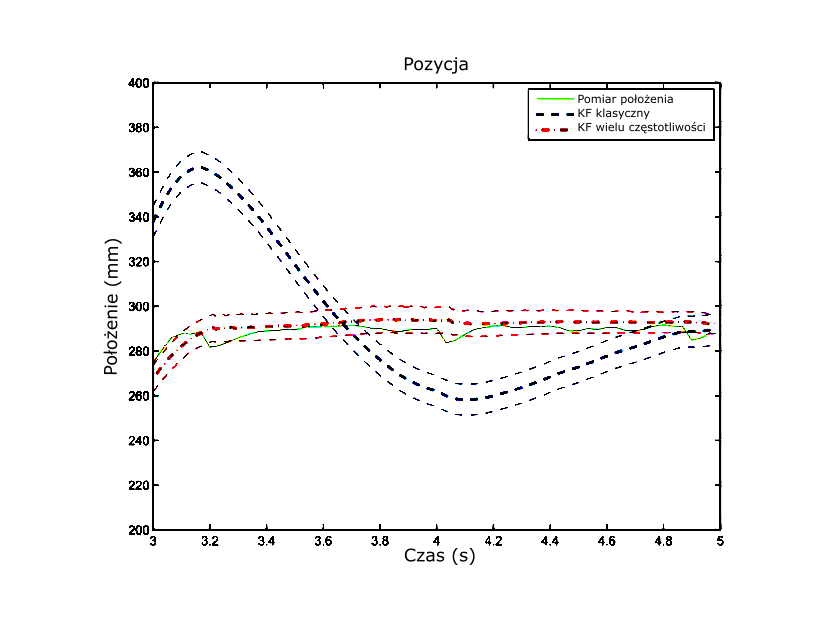
\includegraphics[width=0.95\textwidth]{images/Fig03.png}	
	\caption{Szacowanie położenia stawu z~użyciem klasycznego filtra Kalmana (niebieski) i~filtru Kalmana dostosowanego do różnych częstotliwości (czerwony) \cite{Murray-Smith2014}}
	\label{fig:literature:feng}
\end{figure}
		
Na podstawie wykresów zamieszczonych w~artykule Fanga i~Murray-Smitha można oszacować, że zaproponowana przez nich metoda określa pozycję stawów z~dokładnością $1.5 cm$ -- $2 cm$. Opublikowane diagramy pokazują jedynie wykresy wygenerowane przez zaledwie $5s$, więc problematyczne staje się oszacowanie jak zachowa się ta metoda w~dłuższym okresie. Widać także, że metoda wykorzystująca modyfikację filtru Kalmana uwzględniającą zróżnicowanie częstotliwości łączonych sygnałów szybiej reaguje na zmiany w~wykonywanym ruchu niż metoda oparta o~klasyczną implementację filtru Kalmana (ma mniejszą bezwładność).\\

W 2013 roku Helten et al. \cite{Helten2013} zaproponował połączenie ze sobą sygnałów z~IMU oraz mapy głębi wyznaczonej przez kontroler Kinect. Dane uzyskane z~obu źródeł pozwalają na zbudowanie mapy widoczności poszczególnych części ciała. Informacje zawarte w~tej mapie pozwalają z~koleji wygenerować model ciała odzwierciedlający pozę w~jakiej znajduje się śledzona postać. Wygenerowanie modelu ciała śledzonej postaci pozwala na przeprowadzenie klasyfikacji tego modelu na podstawie wcześniej zdefiniowanego treningowego zbioru zawierającego modele ciała w~określonych, nazwanych pozach. Istotną cechą metody polegającej na klasyfikacji pozy w~jakiej znajduje się śledzona postać był brak możliwości określenia położenia poszczególnych stawów, a~jedynie monitorowanie aktualnej aktywności śledzonej postaci. Dzięki temu można było określić czy dana osoba stoi, chodzi, czy siedzi, a~to z~kolei zapewniło, że metoda zaproponowana przez zespół Thomasa Heltena mogła być z~powodzeniem zastosowana w~systemach nadzorujących np. zachowanie osób starszych. W~związku z~tym metoda ta nie może być porównywana z~takimi metodami jak choćby opisana powyżej metoda zaproponowana przez Bo et al. \cite{Bo2011a}, natomiast autorzy porównali ją z~analogicznymi metodami rozpoznającymi pozy człowieka np. Ganapathi et al. \cite{Ganapathi2010} czy Baak et al. \cite{Baak2011}. Według opisu zamieszczonego w~omawianym artykule, autorzy wskazali, że uzyskane przez nich rezulataty prawidłowego rozponania póz oraz wyznaczenia na ich podstawie modelu szkieletowego było nie gorsze niż innych, podobnych metod opisanych w~literaturze dla wybranego zestawu 6 póz, wśród których były m.in. obroty czy kopnięcia. Jako miarę określającą dokładność dopasowania, zdefiniowano błąd wyznaczenia wybranych 16 stawów uproszczonego modelu szkieletowego, jaki udało się wyznaczyć na podstawie rozpoznanej pozy, względem modelu szkieletowego otrzymanego w~wyniku śledzenia póz optycznym systemem śledzenia ruchu z~markerami firmy PhaseSpace. Średni błąd wyznaczania stawów przez metodę proponowaną przez zespół Thomasa Heltena wyniósł około $75mm$ co stanowiło poprawę o~blisko $50\%$ względem metody o~największym średnim błędzie wśród metod porównywanych w~omawianym artykule.\\
		
Ostatnią z~przytoczonych metod, ujętych w~literaturze i~dyskutowanych w~niniejszej pracy jest metoda zaproponowana w~artykule Kalkbrenner et al. \cite{Kalkbrenner2014}. Autorzy w~swojej metodzie wykorzystali dwa filtry łączące dane uzyskane za pomocą kontrolera Kinect oraz urządzeń pomiarowych opartych o~czujniki inercyjne. Pierwszym z~nich jest filtr zaproponowany przez Sebastiana Madgwicka \cite{Kalkbrenner2014}, drugim -- liniowy filtr Kalmana. Filtr Madgwicka\footnote{Opis filtru można znaleźć w~dodatku \ref{chap:appx:filters}.} pozwala na wyznaczanie orientacji urządzeń pomiarowych w~dwóch osiach dla czujników inercyjnych: akcelerometru i~żyroskopu oraz w~trzech dla czujników inercyjnych wspartych przez magentometr. Implementacja filtru przygotowana przez jego twórcę operowała na kwaternionach, co jest niewątpliwym ułatwieniem dla dalszych przekształceń. Jest to o~tyle istotne, że metoda zaproponowana przez Kalkbrennera wymaga, na podstawie wyniku uzyskanego za pomocą filtru Madgwicka oraz modelu długości kości, wyznaczenia pozycji kolejnych stawów  w~analogiczny sposób jaki ma miejsce przy budowaniu hierarchicznego modelu szkieletowego ciała człowieka. Po wyznaczeniu pozycji stawów (w przypadku dyskutowanego artykułu wyznaczane są jedynie stawy jednej ręki: barkowy, jako korzeń, łokciowy oraz nadgarstkowy) były one łączone z~analogicznymi pozycjami stawów otrzymanymi z~Kinecta za pomocą liniowego filtru Kalmana. 
		
Warto tutaj dodać, że autorzy uzależnili wartość współczynnika Kalmana $K$ (ang. \emph{Kalman gain}) od wartości przemieszczenia stawów $\delta s$ w~modelu szkieletowym Kinecta. Jeśli przemieszczenie to pomiędzy kolejnymi pomiarami było zbyt duże, oznaczało to utratę śledzenia i~brak wiarygodności pomiarów, a~co za tym idzie obniżenie istotności tych danych w~trakcie łączenia. Jako graniczną wartość zbyt dużego przemieszczenia się stawu ($\delta s = [\delta s_x, \delta s_y, \delta s_z]$), po której następowało ponowne wyznaczenie współczynnika Kalmana, autorzy przyjeli wartość $15cm$. W~sytuacji kiedy przemieszczenie się stawu pomiędzy kolejnymi pomiarami przekroczyło tę wartość graniczną następowało ponowne wyznaczenie najpierw macierzy kowariancji kontrolera Kinect $R$, a~następnie współczynnika Kalmana $K$, który wykorzystywał tę macierz odpowiednio według wzorów \eqref{eq:kalman:matrixR} i~\eqref{eq:kalman:gain}.
%[Fixed]w poniższych wzorach nie jest wyjaśniony symbol s_x, s_y, s_z
\begin{equation}
	R = 
	\begin{pmatrix}
		R_x & 0   & 0   \\
		0   & R_y & 0   \\
		0   & 0   & R_z 
	\end{pmatrix} +
	\begin{pmatrix}
		\delta s_x^2 & 0            & 0            \\
		0            & \delta s_y^2 & 0            \\
		0            & 0            & \delta s_z^2 
	\end{pmatrix} * \kappa
	\label{eq:kalman:matrixR}
\end{equation}
		
\begin{equation}
	K = P * H^T * (H * P * H^T +R)^-1
	\label{eq:kalman:gain}
\end{equation}
gdzie:
\begin{conditions}
	H& macierz jednostkowa\\
	R& macierz kowariancji kontrolera Kinect\\
	P& macierz kowariancji czujników inercyjnych\\
	K& współczynnik Kalmana.
\end{conditions}
		
Wartość współczynnika $\kappa$ we wzorze \eqref{eq:kalman:matrixR} została przez autorów artukułu wyznaczona empirycznie na $15$.
		
Twórcy omawianej metody podali wartość średniego odchylenia wyznaczania położenia wybranych stawów na $\pm 2.2cm$ wobec $\pm 5.5cm$ dla kontrolera Kinect pracującego samodzielnie. Z opisu zaproponowanej metody wynika, że dla wyznaczenia pozycji stawów na podstawie IMU, model długości poszczególnych kości pobrany był wprost z~danych Kinecta. Z jednej strony ułatwiło to późniejsze złączenie ze sobą pozycji stawów wyznaczonych przez Kinecta oraz wyznaczonych na podstawie pomiarów czujników inercyjnych, ponieważ jedyna różnica pomiędzy rzeczonymi stawami wynika z~orientacji kości łączących śledzone stawy. Z drugiej zaś strony, oszacowanie długości kości przez kontroler Kinect jest niedokładne i~zmienia się niemal w~każdej klatce pomiarowej, więc unimożliwiało to wyznaczenie prawdziwego modelu szkieletowego, w~którym długości poszczególnych kości odpowiadałyby prawdziwym długościom.\\
		
Na tej podstawie zasadnym wydaje się wprowadzenie modelu szkieletowego, którego długości poszczególnych kości miałyby stałe wartości. Wymagałoby to jednak wcześniejszego dokonania pomiarów poszczególnych kości w~celu zbudowania takiego modelu. Eliminując zaszumienie ostatecznych wyników przez zmienność długości kości, łączenie danych z~urządzenia Kinect i~czujników inercyjnych powinno odbywać się z~wykorzystaniem informacji o~tym, w~jakiej orientacji znajdują się poszczególne kości. Estymacja taka dostępna jest wśród danych udostępnianych przez oprogramowanie kontrolera Kinect, a~także jest dostępne w~wyniku działania urządzeń pomiarowych opartych o~czujniki inercyjne. Następnie wykorzystanie informacji o~obrotach, z~przygotowanym wcześniej modelem szkieletowym, pozwala wyznaczyć położenie poszczególnych stawów. Można przypuszczać, że wprowadzenie modelu szkieletowego o~stałych długościach kości i~wykorzystanie informacji o~ich obrocie da większą dokładność wyznaczania pozycji stawów niż bezpośrednie łączenie ze sobą pozycji stawów wyznaczonych w~dwóch modelach szkieltowych, dla każdego z~urządzeń pomiarowych mających zmienne długości kości. Powyższe spostrzeżenia stanowią podstawową przesłankę budowy nowej, auroskiej hybrydowej metody śledzenia ruchu kończyn.
\chapter{Hybrydowa metoda śledzenia ruchu człowieka}\label{chap:hybrid}

Prezentowana w~niniejszej dysertacji hybrydowa metoda śledzenia ruchu człowieka, wykorzystuje dwa rodzaje urządzeń pomiarowych: kontroler Microsoft Kinect oraz czujniki inercyjne - akcelerometr i~żyroskop, których charakterystyki zostały przedstawione w~rozdziale \ref{chap:characteristics}. Mając na uwadze dokładność danych przesyłanych przez każde z~zastosowanych urządzeń pomiarowych oraz ograniczenia w~ich działaniu, takie jak wrażliwość na występowanie okluzji sensora głębi, czy ograniczona liczba stopni swobody układów inercyjnych, opracowana przez autora hybrydowa metoda śledzenia ruchu człowieka umożliwia ograniczenie wpływu niedoskonałości każdego ze składowych urządzeń. Autorskie połączenie danych (\emph{ang. data fusion}) z~kontrolera Kinect i~czujników inercyjnych poprawia precyzję szacowania położenia stawów, a~co za tym idzie wpływa korzystnie na precyzję śledzenia wykonywanego przez użytkownika ruchu. Ograniczenie wpływu niedoskonałości każdego z~wykorzystanych urządzeń pomiarowych na dokładność śledzenia ruchu możliwe jest dzięki temu, że są one względem siebie w~pewnym stopniu komplementarne to znaczy, że niedoskonałości występujące w~jednym urządzeniu i~wpływające, na przykład, na przerwy w śledzeniu ruchu w~jednej z~płaszczyzn, mogą zostać ograniczone przez wykorzystanie możliwości śledzenia ruchu w~tej płaszczyźnie przez drugie z~urządzeń.\\
Proces łączenia danych uzyskanych z~kontrolera Kinect i~z czujników inercyjnych podzielony został na kilka etapów, z~których część jest wykonana jedynie na samym początku, a~część jest powtarzana w~trakcie śledzenia ruchu. Schemat kolejnych kroków przetwarzania danych prezentuje diagram na rysunku \ref{fig:hybrid:stepsSequence}. Kroki te zostały omówione w~dalszej części niniejszego rozdziału.\\

\begin{figure}[!htb]
	\scalebox{0.7}{
		\begin{tikzpicture} [
		scale=0.8,
		auto,
		decision/.style = { diamond, draw=black, thick, fill=black!20,
			text width=5em, text badly centered,
			inner sep=1pt, rounded corners },
		block/.style    = { rectangle, draw=black, thick, 
			fill=black!20, text width=10em, text centered,
			rounded corners, minimum height=2em },
		line/.style     = { draw, thick, ->, shorten >=2pt },
	]
	% Define nodes in a~matrix
	\matrix [column sep=5mm, row sep=10mm] {
		\node [block] (block1) {Inicjalizacja czujników inercyjnych}; \\                    
		\node [block] (block2) {Inicjalizacja filtrów łączących dane z~akcelerometru i~żyroskopu}; \\
		\node (null1) {};  \\
		\node [block] (block3) {Odszumienie danych z~czujników inercyjnych oraz z~kontrolera Kinect}; \\
		\node [decision] (inSync) {Czy dane zostały zsynchronizowane?}; \\
		\node [block] (block4) {Synchronizacja czasowa sygnałów z~czujników inercyjnych oraz z~kontrolera Kinect}; \\
		\node [block] (block5) {Łączenie danych z~czujników inercyjnych oraz z~kontrolera Kinect}; \\
		\node [block] (block6) {Oszacowanie położenia stawów}; \\                    
	};
	% connect all nodes defined above
	\begin{scope} [every path/.style=line]
		\path (block1)        --    (block2);
		\path (block2)      --   (block3);
		\path (block3)      --    (inSync);
		\path (inSync)  --++  (-3,0) node [near start] {Tak} |- (block5);
		\path (inSync)  --++  (3,0) node [near start] {Nie} |- (block4);
		\path (block4)      --    (block5);
		\path (block5)      --    (block6);
		\path (block6)      --++  (4,0) node [near start] {} |-  (null1);
	\end{scope}			
\end{tikzpicture}
	}
	\caption{Algorytm przetwarzania danych w~autorskiej metodzie łączenia danych (źródło: badania własne)}
	\label{fig:hybrid:stepsSequence}						
\end{figure}
\begin{figure}[!htb]
	\centering			
	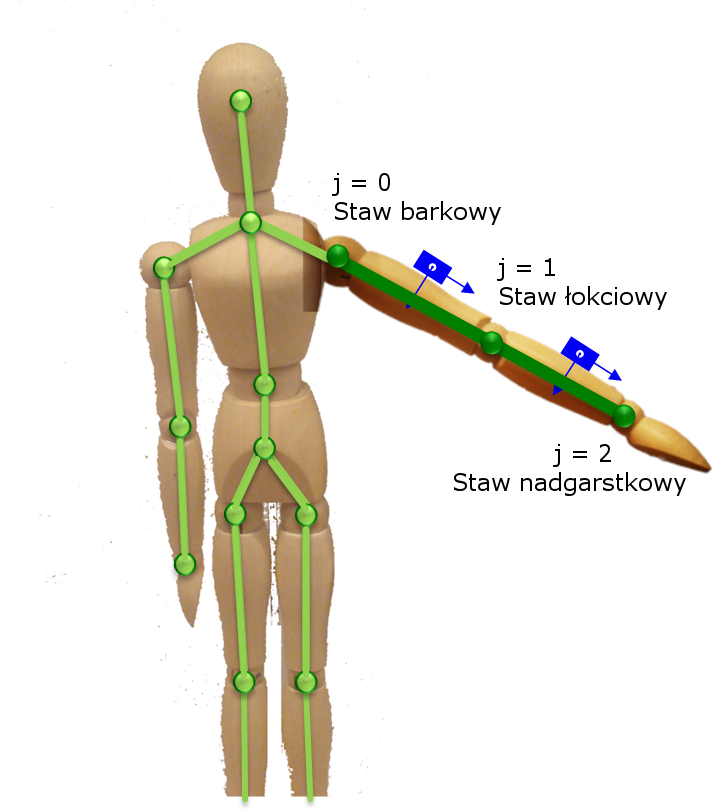
\includegraphics[width=0.75\textwidth]{images/joints.png}
	\caption{Przykład hierarchii stawów dla modelu szkieletowego ręki (źródło: opracowanie własne)}		
	\label{fig:hybrid:jointsHierarchy}		
\end{figure}

		
Zadaniem, omawianej w~niniejszym rozdziale, hybrydowej metody śledzenia ruchu człowieka jest oszacowanie w~chwili czasu $t$ położenia wybranego stawu $j$ szkieletu postaci ($P^F_{j,t} = [p^F_{j,x}, p^F_{j,y}, p^F_{j,z}]_t$, $F$ -- \emph{ang. Fused})  w~przestrzeni trójwymiarowej opisanej w referencyjnym układzie współrzędnych $X Y Z$, tożsamym z~układem współrzędnych kontrolera Kinect. W zakresie pojedynczego modułu inercyjnego szacowanie położenia stawu odbywa się na podstawie pomiaru sił działających na akcelerometr w~każdej z~trzech osi ($A = [a_x, a_y, a_z]$), pomiaru prędkości kątowych, z~jakimi porusza się żyroskop względem każdej z~osi ($G = [g_x, g_y, g_z]$) oraz aktualnej temperatury pracy czujników inercyjnych ($T$). Pomiary uzyskane z~akcelerometru oraz żyroskopu wyrażone są w~układzie współrzędnych modułu inercyjnego (rys.~\ref{fig:characteristics:imu:space}). W~przypadku kontrolera Kinect pobierane są pozycje dwóch stawów: stawu $j$, którego pozycja będzie szacowana ($P^K_{j} = [p^K_{j,x}, p^K_{j,y}, p^K_{j,z}]$, $K$--Kinect) oraz stawu $j-1$ ($P^K_{j-1} = [p^K_{j-1,x},p^K_{j-1,y}, p^K_{j-1,z}]$), będącego jego rodzicem w~modelu szkieletowym Kinecta (rys.~\ref{fig:hybrid:jointsHierarchy}). Fuzja danych z~czujników inercyjnych ($A$ oraz $G$) oraz z~kontrolera Kinecta ($P^K_j$) pozwala oszacować pozycję stawu $j$ w~danej chwili $t$ ($P^F_{j,t}$) i~odbywa się z~pewnym interwałem czasowym $\Delta t$, określającym czas pomiędzy kolejnymi aktualizacjami pomiarów kontrolera Kinect, a~będącym jednocześnie interwałem czasowym dla procesu decymacji sygnału urządzeń inercyjnych. Dodatkowymi parametrami wykorzystywanymi w~procesie łączenia danych z~modułu inercyjnego z~pomiarami Kinecta są pozycje obu stawów barkowych uzyskane za pomocą kontrolera Kinect ($P^K_{sh_L,t}, P^K_{sh_R,t}$). Pozwalają one oszacować:

\begin{enumerate}
	\item jak śledzona postać jest obrócona względem Kinecta,
	\item pozycję stawu rodzica ($P^F_{j-1,t}$) w~globalnym układzie współrzędnych, będącą wynikiem osobnej fuzji danych,
	\item długość kości $l$, na której umieszczony jest moduł inercyjny.
\end{enumerate}

Biorąc pod uwagę powyższe, oszacowanie pozycji wybranego stawu $j$, w hybrydowej metodzie śledzenia ruchu człowieka, można wyrazić za pomocą uogólnionego wzoru \ref{eq:methodFormula}, którego szczegółowy kształt zostanie przedstawiony w dalszej części pracy.
		
\begin{equation}
	P^F_{j,t} = [p_{j,x}^F,p_{j,y}^F,p_{j,z}^F]_t = f(A,G,T,P_{j-1,t}^K,P_{j,t}^K,\Delta t, P^F_{j-1,t}, P^K_{sh_L,t},P^K_{sh_R,t},l) 
	\label{eq:methodFormula}
\end{equation}
%A - akcelerometr - potrzebny do madgwicka
%G - żyroskop - potrzebny do madgwicka
%T - temperatura - potrzebna do korekty akcelerometru
%P_j^K - staw śledzony pobrany z~Kinecta, potrzebny do fuzji
%P_j-1^K - staw rodzica pobrany z~kinecta
%P^F_{j-1,t} - staw rodzica już po fuzji. względem niego będzie wyrównany punkt wynikowy
% \Delta t - różnica czasu pomiędzy kolejnymi łączeniami dla filtru madgwicka
%------
%l - długość wybranej kości żeby wyznaczyć położenie stawu po fuzji
%P_shR^K, P_shL^K - położenie stawów barkowych z~kinecta do obliczenia orientacji względem kamery 
		
		
Wzór \ref{eq:methodFormula} odnosi się do każdego modułu inercyjnego zbudowanego z~pary czujników: akcelerometru i~żyroskopu, umieszczonego na ciele pomiędzy dwoma kolejnymi stawami, których pozycje oszacowane przez kontroler Kinect są argumentami metody. W~przypadku śledzenia ruchu więcej niż jednego stawu, powyższą metodę należy wykonać zgodnie z~ustaloną hierarchią stawów rozpoczynając od przyjętego korzenia. Oszacowana, w~wyniku fuzji, pozycja stawu $P^F_{j,t}$ określa jego położenie w~globalnym układzie współrzędnych prezentowanego systemu śledzenia ruchu, który pokrywa się z~układem współrzędnych kontrolera Kinect.
		
\section{Format danych używany przez urządzenia pomiarowe}
\subsection{Kontroler Kinect}
Kontroler Kinect w~ramach pakietu pomiarów, rejestrowanego z~częstotliwością $30 Hz$, udostępnia 3 kategorie danych dotyczących obserwowanej sceny: obraz z~kamery RGB, mapę głębi sceny oraz model szkieletowy postaci widocznej na scenie. Kontroler Kinect może jednocześnie zrekonstruować modele szkieletowe dwóch postaci i~śledzić ich kolejne pozy, rejestrując tym samym ich ruch. W~zależności od potrzeb, aplikacja wykorzystująca kontroler Kinect może uzyskać wszystkie 3 kategorie danych jednocześnie lub wybrać tylko te z~nich, które potrzebuje do swojego działania. Opisywana w~niniejszej dysertacji hybrydowa metoda śledzenia ruchu kończyn człowieka bazuje na informacji dotyczącej modelu szkieletowego śledzonej postaci wybierając z~pełnego modelu tylko informacje związane z~wybranymi stawami reprezentującymi śledzoną kończynę oraz te, na podstawie których można określić wiarygodność pomiarów uzyskanych za pomocą kontrolera Kinect. Na przykład przy śledzeniu ruchu prawej ręki są to oba stawy barkowe, prawy staw łokciowy oraz prawy staw nadgarstkowy. Każdy staw $j$ reprezentowany jest przez trzy współrzędne ($P^K_j = [p^K_{j,x}, p^K_{j,y}, p^K_{j,z}]$) określające jego położenie w~przestrzeni w~układzie współrzędnych kontrolera Kinect oraz informacje o~stanie śledzenia tego stawu: \emph{Tracked}, \emph{Interferred} albo \emph{NotTracked}. Na podstawie współrzędnych stawów barkowych postaci obliczany jest kąt obrotu sylwetki względem Kinecta (wzór \ref{eq:characteristics:kinect:bodyRotationAngle}). Dodatkowo każdy pakiet danych zawiera informacje o~swoim numerze, znacznik czasu wygenerowany przez kontroler Kinect oraz godzinę odebrania danych na komputerze, do którego podłączone jest to urządzenie.
		
\subsection{Czujniki inercyjne}
Moduły inercyjne (IMU1 i~IMU2) zbudowane zostały z~czujników inercyjnych: akcelerometru i~żyroskopu, podłączonych bezpośrednio do jednostki centralnej opartej na platformie Arduino. Częstotliwość odczytu danych z~czujników kontrolowana jest przez zewnętrzny moduł zegara (RTC DS3230), który również został podłączony bezpośrednio do Arduino{\footnote{Arduino -- platforma programistyczna dla systemów wbudowanych, \url{www.arduino.cc}}}. Zadaniem jednostki centralnej jest odczyt danych z~czujników, sformatowanie ich i~wysłanie z~wykorzystaniem technologii Bluetooth (BT HC-05) do komputera PC, gdzie następuje dalsze ich przetwarzanie (uproszczony schemat urządzenia do pomiaru danych inercyjnych\footnote{Urządzenie do pomiaru danych inercyjnych jest urządzeniem zaprojektowanym i~wykonanym przez autora niniejszej dysertacji.} przedstawia rys. \ref{fig:device:circuitDiagram}). Odczyt pakietu danych z~pojedynczego modułu obejmuje:

\begin{enumerate}
	\item zestaw pomiarów udostępnionych przez żyroskop (trzy wartości obrotu $G = [g_x, g_y, g_z]$, po jednej dla każdej z~osi),
	\item zestaw pomiarów z~akcelerometru (trzy wartości przyspieszenia $A = [a_x, a_y, a_z]$),
	\item pomiar temperatury czujników $T$.
\end{enumerate}

Wszystkie pomiary przesyłane są jako 16-bitowe liczby całkowite ze znakiem i~pomiary ze wszystkich podłączonych modułów wysyłane są do komputera PC jednocześnie. Przesyłane wartości muszą być następnie skonwertowane do jednostek odpowiadających wielkościom fizycznym mierzonym przez poszczególne czujniki. Dla żyroskopu są to stopnie na sekundę ($\degree/s$), dla akcelerometru -- jednostki przyspieszenia grawitacyjnego ($g$), które można również przeliczyć na jednostki przyspieszenia $m/_{s^2}$, a~dla temperatury stopnie Celsjusza ($\degree C$). W~przypadku danych z~czujników inercyjnych konwersja polega na podzieleniu wartości bezpośredniego odczytu z~czujników przez współczynniki odpowiednie dla zakresu pracy tych czujników. Tabele \ref{tab:hybrid:accRangeFactors} oraz \ref{tab:hybrid:gyroRangeFactors} przedstawiają zestawienie współczynników konwersji $f_A$ i~$f_G$ wykorzystywanych do konwersji pomiarów odpowiednio z~akcelerometru i~żyroskopu. Jak już zostało to zaznaczone wcześniej, w~trakcie prowadzonych eksperymentów badawczych, zakres pracy akcelerometru został ustalony na $\pm4g$, natomiast żyroskopu na $\pm500\degree/s$. Jako zakresy pracy czujników modułów inercyjnych przyjęto podobne wartości do tych zastosowanych w~kontrolerze ruchu Nintendo Wii Remote Plus. 
	
\begin{figure}[!htb]
		\captionsetup{singlelinecheck=off}
	\centering
	\rotatebox{-90}{
		\begin{figure}[!htp]
	\centering
	\begin{tikzpicture}
		\draw  (-3,5) rectangle (3,-5); % board
		\draw  (-2,4.75) rectangle (-1.5,4); % DC in
		\node [font=\tiny]   at(-1.75, 3.8){DC IN};
		\draw[fill=green!20]  (-0.5,4.75) rectangle (0.25,4.5); % USB 1
		\node [font=\tiny]   at(-0.1, 4.62){USB1};
		\draw  (0.75,4.75) rectangle (1.5,4.5); % USB 2
		\node [font=\tiny]   at(1.1, 4.62){USB2};
		\draw (2.5,3.75) rectangle (2.75,1.25);%SCL1
		\draw (2.5,3.5) -- (2.75, 3.5);%SDA1
		\draw (2.5,3.25) -- (2.75, 3.25);%AREF
		\draw (2.5,3) -- (2.75, 3);%GND
		\draw (2.5,2.75) -- (2.75, 2.75);%D13
		\draw (2.5,2.5) -- (2.75, 2.5);%D12
		\draw (2.5,2.25) -- (2.75, 2.25);%D11
		\draw (2.5,2) -- (2.75, 2);%D10
		\draw (2.5,1.75) -- (2.75, 1.75);%D09
		\draw (2.5,1.5) -- (2.75, 1.5);%D08
		\draw  (2.5,1) rectangle (2.75,-1);%D07
		\draw (2.5,0.75) -- (2.75, 0.75);%D06
		\draw (2.5,0.5) -- (2.75, 0.5);%D05
		\draw (2.5,0.25) -- (2.75, 0.25);%D04
		\draw (2.5,0) -- (2.75, 0);%D03
		\draw (2.5,-0.25) -- (2.75, -0.25);%D02
		\draw (2.5,-0.5) -- (2.75, -0.5); %TX0 -> 1
		\draw (2.5,-0.75) -- (2.75, -0.75); %RX0 -> 2
		\draw  (2.5,-1.25) rectangle (2.75,-3.25); %TX3
		\draw (2.5,-1.5) -- (2.75, -1.5); %RX3
		\draw (2.5,-1.75) -- (2.75, -1.75); %TX2
		\draw (2.5,-2) -- (2.75, -2); %RX2
		\draw (2.5,-2.25) -- (2.75, -2.25); %TX1
		\draw (2.5,-2.5) -- (2.75, -2.5); %RX1
		\draw (2.5,-2.75) -- (2.75, -2.75); %SDA
		\draw (2.5,-3) -- (2.75, -3); %SCL
		\draw  (-2.75,3.25) rectangle (-2.5,1.25);
		\draw (-2.75,3) -- (-2.5, 3);%IOREF
		\draw (-2.75,2.75) -- (-2.5, 2.75);%RESET
		\draw (-2.75,2.5) -- (-2.5, 2.5);%3.3V
		\draw (-2.75,2.25) -- (-2.5, 2.25);%5V
		\draw (-2.75,2) -- (-2.5, 2);%GND
		\draw (-2.75,1.75) -- (-2.5, 1.75);%GND
		\draw (-2.75,1.5) -- (-2.5, 1.5);%VIN
		\draw  (-2.75,1) rectangle (-2.5,-1); %A0
		\draw (-2.75,0.75) -- (-2.5, 0.75);%A1
		\draw (-2.75,0.5) -- (-2.5, 0.5);%A2
		\draw (-2.75,0.25) -- (-2.5, 0.25);%A3
		\draw (-2.75,0) -- (-2.5, 0);%A4
		\draw (-2.75,-0.25) -- (-2.5, -0.25);%A5
		\draw (-2.75,-0.5) -- (-2.5, -0.5); %A6
		\draw (-2.75,-0.75) -- (-2.5, -0.75); %A7
		\draw  (-2.75,-1.25) rectangle (-2.5,-3.25);%A08
		\draw (-2.75,-1.5) -- (-2.5, -1.5); %TX0 -> 1
		\draw (-2.75,-1.75) -- (-2.5, -1.75); %RX0 -> 2
		\draw (-2.75,-2) -- (-2.5, -2);%A4
		\draw (-2.75,-2.25) -- (-2.5, -2.25);%A5
		\draw (-2.75,-2.5) -- (-2.5, -2.5); %A6
		\draw (-2.75,-2.75) -- (-2.5, -2.75); %A7
		\draw (-2.75,-3) -- (-2.5, -3);%A4
		\draw  (-2.25,-3.75) rectangle (2.25,-4.25);
		\draw  (-2.25,-4) -- (2.25,-4);
		\draw  (-2,-3.75) -- (-2,-4.25);
		\draw  (-1.75,-3.75) -- (-1.75,-4.25);
		\draw  (-1.5,-3.75) -- (-1.5,-4.25);
		\draw  (-1.25,-3.75) -- (-1.25,-4.25);
		\draw  (-1,-3.75) -- (-1,-4.25);
		\draw  (-0.75,-3.75) -- (-0.75,-4.25);
		\draw  (-0.5,-3.75) -- (-0.5,-4.25);
		\draw  (-0.25,-3.75) -- (-0.25,-4.25);
		\draw  (0,-3.75) -- (0,-4.25);
		\draw  (0.25,-3.75) -- (0.25,-4.25);
		\draw  (0.5,-3.75) -- (0.5,-4.25);
		\draw  (0.75,-3.75) -- (0.75,-4.25);
		\draw  (1,-3.75) -- (1,-4.25);
		\draw  (1.25,-3.75) -- (1.25,-4.25);
		\draw  (1.5,-3.75) -- (1.5,-4.25);
		\draw  (1.75,-3.75) -- (1.75,-4.25);
		\draw  (2,-3.75) -- (2,-4.25);
		%IMU1
		\draw  [fill=blue!20](4.2,4.4) rectangle (6,3.4);
		\draw  [fill=white](4.3,4.3) rectangle (4.5,3.5);
		\draw  (4.3,4.1) -- (4.5,4.1);
		\draw  (4.3,3.9) -- (4.5,3.9);
		\draw  (4.3,3.7) -- (4.5,3.7);
		%IMU2
		\draw  [fill=blue!20](4.2,-2.8) rectangle (6,-3.8);
		\draw  [fill=white](4.3,-2.9) rectangle (4.5,-3.7);
		\draw  (4.3,-3.1) -- (4.5,-3.1);
		\draw  (4.3,-3.3) -- (4.5,-3.3);
		\draw  (4.3,-3.5) -- (4.5,-3.5);
		%BT
		\draw  [fill=blue!20](4.8,-1) rectangle (6.6,-2);
		\draw  [fill=white](4.9,-1.1) rectangle (5.1,-1.9);
		\draw  (4.9,-1.3) -- (5.1,-1.3);
		\draw  (4.9,-1.5) -- (5.1,-1.5);
		\draw  (4.9,-1.7) -- (5.1,-1.7);
		%RTC
		\draw  [fill=blue!20](4.2,-4.2) rectangle (6,-5.2);
		\draw  [fill=white](4.3,-4.3) rectangle (4.5,-5.1);
		\draw  (4.3,-4.5) -- (4.5,-4.5);
		\draw  (4.3,-4.7) -- (4.5,-4.7);
		\draw  (4.3,-4.9) -- (4.5,-4.9);
		%LCD
		\draw  (4.8,1.6) rectangle (6.8,-0.375);
		\draw  (4.9,1.5) rectangle (5.15,-0.25);
		\draw (4.9,1.25) -- (5.15, 1.25); 
		\draw (4.9,1) -- (5.15, 1); 
		\draw (4.9,0.75) -- (5.15, 0.75);
		\draw (4.9,0.5) -- (5.15, 0.5);
		\draw (4.9,0.25) -- (5.15, 0.25);
		\draw (4.9,0) -- (5.15, 0);
		\node[left, font=\tiny] (SCL1) at (2.625,3.625) {SCL1$\quad$};
		\node[left, font=\tiny] (SDA1) at (2.625,3.375) {SDA1$\quad$};
		\node[left, font=\tiny] (GND) at (2.625,2.875) {GND$\quad$};
		\node[left, font=\tiny] (D07) at (2.625,0.875) {D07$\quad$};
		\node[left, font=\tiny]  (D06) at (2.625,0.625) {D06$\quad$};
		\node[left, font=\tiny]  (D05) at (2.625,0.375) {D05$\quad$};
		\node[left, font=\tiny]  (D04) at (2.625,0.125) {D04$\quad$};
		\node[left, font=\tiny]  (D03) at (2.625,-0.125) {D03$\quad$};
		\node[left, font=\tiny]  (TX1) at (2.625,-2.375) {TX1$\quad$};
		\node[left, font=\tiny]  (RX1) at (2.625,-2.625) {RX1$\quad$};
		\node[left, font=\tiny]  (SDA) at (2.625,-2.875) {SDA$\quad$};
		\node[left, font=\tiny]  (SCL) at (2.625,-3.125) {SCL$\quad$};
		\node (GND3) at (-2.125,-3.875) {};
		\node[above left, font=\tiny] (GND4) at (-2.125,-4.125) {GND$\quad$};
		\node[below right, font=\tiny] (50V3) at (2.125,-3.875) {$\quad$5V};
		\node[right, font=\tiny] (50V4) at (2.125,-4.125) {};
		\node (33V)at (-2.625,2.375) {};
		\node[left, font=\tiny] at (-2.725,2.375) {$\quad$3.3V};
		\node (50V) at (-2.625,2.125) {};
		\node[left, font=\tiny]  at (-2.725,2.125) {$\quad$5V};
		\node[right, font=\tiny]  (GND1) at (-2.625,1.875) {$\quad$GND};
		\node[right, font=\tiny]  (GND2) at (-2.625,1.625) {$\quad$GND};
		\node(IMU1VCC) at (4.4,4.2) {};
		\node(IMU1SCL) at (4.4,4.0) {};
		\node(IMU1SDA) at (4.4,3.8) {};
		\node(IMU1GND) at (4.4,3.6) {};
		\node[right, font=\tiny] at (4.5,4.2) {VCC};
		\node[right, font=\tiny] at (4.5,4) {SCL};
		\node[right, font=\tiny] at (4.5,3.8) {SDA};
		\node[right, font=\tiny] at (4.5,3.6) {GND};
		\node[rotate=90, font=\tiny] at (5.6,3.9) {IMU1};
		\node(IMU2VCC) at (4.4,-3) {};
		\node(IMU2SCL) at (4.4,-3.2) {};
		\node(IMU2SDA) at (4.4,-3.4) {};
		\node(IMU2GND) at (4.4,-3.6) {};
		\node[right, font=\tiny] at (4.5,-3) {VCC};
		\node[right, font=\tiny] at (4.5,-3.2) {SCL};
		\node[right, font=\tiny] at (4.5,-3.4) {SDA};
		\node[right, font=\tiny] at (4.5,-3.6) {GND};
		\node[rotate=90, font=\tiny] at (5.6,-3.3) {IMU2};
		\node(BTGND) at (5,-1.2) {};
		\node(BTVCC) at (5,-1.4) {};
		\node(BTRX) at (5,-1.6) {};
		\node(BTTX) at (5,-1.8) {};
		\node[right, font=\tiny] at (5.1,-1.2) {GND};
		\node[right, font=\tiny] at (5.1,-1.4) {VCC};
		\node[right, font=\tiny] at (5.1,-1.6) {RX};
		\node[right, font=\tiny] at (5.1,-1.8) {TX};
		\node[rotate=90, font=\tiny, align=center] at (6.1,-1.5) {BT \\ HC-05};
		\node(RTCSDA) at (4.4,-4.4) {};
		\node(RTCSCL) at (4.4,-4.6) {};
		\node(RTCGND) at (4.4,-4.8) {};
		\node(RTCVCC) at (4.4,-5) {};
		\node[right, font=\tiny] at (4.5,-4.4) {SDA};
		\node[right, font=\tiny] at (4.5,-4.6) {SCL};
		\node[right, font=\tiny] at (4.5,-4.8) {GND};
		\node[right, font=\tiny] at (4.5,-5) {VCC};
		\node[rotate=90, font=\tiny, align=center] at (5.6,-4.7) {RTC \\ DS3230};
		\node (LCDGND) at (5.025,1.375) {};
		\node (LCDVCC) at (5.025,1.125) {};
		\node (LCDD07) at (5.025,0.875) {};
		\node (LCDD06) at (5.025,0.625) {};
		\node (LCDD05) at (5.025,0.375) {};
		\node (LCDD04) at (5.025,0.125) {};
		\node (LCDD03) at (5.025,-0.125) {};
		\node[right, font=\tiny] at (5.1,1.375) {GND};
		\node[right, font=\tiny] at (5.1,1.125) {VCC};
		\node[right, font=\tiny] at (5.1,0.875) {SCLK};
		\node[right, font=\tiny] at (5.1,0.625) {DIN};
		\node[right, font=\tiny] at (5.1,0.375) {D/C};
		\node[right, font=\tiny] at (5.1,0.125) {CS};
		\node[right, font=\tiny] at (5.1,-0.125) {RST};
		\node[rotate=90, font=\tiny, align=center] at (6.4,0.625) {LCD};
		\draw(SCL1) --(3.625,3.625) |- (IMU1SCL);
		\draw  (SDA1)--(3.725,3.375)  |-(IMU1SDA);
		\draw  (GND) -- (3.825,2.875)|- (IMU1GND);
		\draw  (50V) --(0,2.125) |- (IMU1VCC);
		\draw  (50V) --(0,2.125)--(0,-1.125)--(4,-1.125) |- (IMU2VCC);
		\draw (SDA) -- (3.8,-2.875) |-(IMU2SDA);
		\draw(SCL) -- (3.6,-3.125) |- (3.72,-3.2) arc(180:0:0.08)--(IMU2SCL);4.4,-3.2
		\draw (GND3) |- (IMU2GND);
		\draw(4,-1.125) |- (BTVCC);
		\draw(TX1) --(3.9,-2.375) arc(180:0:0.1)--(4.2,-2.375) |-(BTRX);
		\draw(RX1) --(3.9,-2.625) arc(180:0:0.1)--(4.4,-2.625) |-(BTTX);
		\draw  (GND) -- (4.125,2.875)|- (BTGND);
		\draw  (4.125,1.375) -- (LCDGND);
		\draw (33V) -- (-0.1,2.375) arc(180:0:0.1)-- (1,2.375) |-(4.025,1.125) arc(180:0:0.1)-- (LCDVCC);
		\draw (D07) --(4.025,0.875) arc(180:0:0.1)-- (LCDD07);
		\draw (D06) --(4.025,0.625) arc(180:0:0.1)-- (LCDD06);
		\draw (D05) --(4.025,0.375) arc(180:0:0.1)--(LCDD05);
		\draw (D04) --(4.025,0.125) arc(180:0:0.1)-- (LCDD04);
		\draw (D03) --(4.025,-0.125) arc(180:0:0.1)-- (LCDD03);
		\draw(3.8,-2.875) --(3.8,-3.5) arc(90:-90:0.1)|-(RTCSDA);
		\draw(3.6,-3.125)--(3.6,-3.5) arc(90:-90:0.1) |-(RTCSCL);
		\draw(3.4,-3.6) |-(RTCGND);
		\draw(50V4) -- (3.2, -4.125) |- (RTCVCC);
		\draw(0.9,2.375)--(0.9,2.6);
		\draw(1,2.375)-|(1.15,2.6);
		\draw(0.9,3.2)|-(SCL1);
		\draw(1.15,3.2) |-(SDA1);
		\draw  (1.05,3.2) rectangle (1.25,2.6);
		\draw  (0.8,3.2) rectangle (1.,2.6);
		\node[font=\tiny, rotate=90] at (0.9,2.9) {4k7$\Omega$};
		\node[font=\tiny, rotate=90] at (1.15,2.9) {4k7$\Omega$};
		\node[font=\tiny] at (0,-2) {Arduino Due};
	\end{tikzpicture}
	\caption{Schemat budowy urządzenia pomiarowego opartego o~komputer Arduino.}
													
	\label{fig:device:circuitDiagram}
\end{figure}
	}
	\caption{Schemat budowy urządzenia pomiarowego opartego o~komputer Arduino (źródło: badania własne). IMU1 i~IMU2 -- Moduły inercyjne, RTC -- moduł zagara oparty o~komponent DS3230, BT -- moduł Bluetooth oparty o~komponent HC-05, LCD -- ekran ciekłokrystaliczny}	
	\label{fig:device:circuitDiagram}
\end{figure}
		
\begin{savenotes}
	\begin{table}[!htb]
		\caption[Współczynniki konwersji bezpośrednich pomiarów akcelerometru (a) i żyroskopu (b) w~zależności od przyjętego zakresu pracy]{Współczynniki konwersji bezpośrednich pomiarów akcelerometru (a) i żyroskopu (b) w~zależności od przyjętego zakresu pracy\footfullcite{footnote:ivenSense:MPU6050}}
		\begin{subtable}{.5\linewidth}
			\centering
			\caption{Akcelerometr}
			\label{tab:hybrid:accRangeFactors} 
			\begin{tabular}{|l|c|}
				\hline
				Zakres pomiaru              & Współczynnik \\ \hline
				$\pm2g$                     & $16384$        \\ \hline
				\rowcolor{black!20} $\pm4g$ & $8192$         \\ \hline
				$\pm8g$                     & $4096$         \\ \hline
				$\pm16g$                    & $2048$         \\ \hline
			\end{tabular}
		\end{subtable}%
		\begin{subtable}{.5\linewidth}
			\centering
			\caption{Żyroskop}
			\label{tab:hybrid:gyroRangeFactors}	
			\begin{tabular}{|l|c|}
				\hline
				Zakres pomiaru                        & Współczynnik \\ \hline
				$\pm250\frac{\degree}{s}$             & $131.0$        \\ \hline
				\rowcolor{black!20} $\pm500\degree/s$ & $65.5$         \\ \hline
				$\pm1000\frac{\degree}{s}$            & $32.8$         \\ \hline
				$\pm2000\frac{\degree}{s}$            & $16.4$         \\ \hline
			\end{tabular}
		\end{subtable} 
	\end{table}
\end{savenotes}	
		
		
Konwersja pomiaru temperatury czujników ($T_{raw}$) do wartości wyrażonej w~$\degree C$ ($T_{deg}$) wymaga zastosowania wzoru \ref{eq:hybrid:tempEquation}

\begin{equation}
	T_{deg} = 36.53 + T_{raw} / 340.0
	\label{eq:hybrid:tempEquation}
\end{equation}

wynikającego ze specyfikacji zastosowanego układu elektronicznego IvenSense MPU-6050. Wartości stałe zastosowane w~tym wzorze związane są z~rozdzielczością pomiarów wykorzystanego w~tym układzie elektronicznym termometru (wartość = 340.0) oraz ze stałego przesunięcia dla temperatury $0 \degree C$ (wartość = 36.53)
				
Do danych pobranych ze wszystkich podłączonych modułów inercyjnych, podobnie jak w~przypadku danych z~Kinecta, dołączone są znaczniki czasowe zarówno ustawiane przez urządzenie, jak i~przez komputer PC w~momencie odbioru danych oraz numeracja kolejnych pakietów danych. Odczyt danych z modułów inercyjnych odbywa się z częstotliwością $100Hz$.
		
\section{Kalibracja}
W proponowanym systemie czujniki inercyjne wymagają kalibracji przy każdym uruchomieniu. Kalibracja Kinecta nie jest wymagana, a~jedyne co należy zrobić to upewnić się, że kąt nachylenia kamery pozwala na obserwację śledzonej postaci.
		
Kalibracja czujników inercyjnych przebiega dwuetapowo w~następującej kolejności:
\begin{enumerate}
	\item {Wyznaczenie współczynników korekty odchylenia pomiarów czujników inercyjnych dla wartości spoczynkowych.} 
	\item {Inicjalizacja filtru Madgwicka wyznaczającego orientację sensora na podstawie danych z~czujników inercyjnych.}
\end{enumerate}
		
Krok pierwszy służy do wyznaczenia macierzy współczynników korekty ($cor = [cor_A \quad cor_G]^T = [[c_{AX},c_{AY},c_{AZ}]\quad [c_{GX},c_{GY},c_{GZ}]]^T $) pomiarów spoczynkowych ($G, A$) dla każdego modułu inercyjnego indywidualnie. W~trakcie tego kroku kalibrowane czujniki należy umieścić możliwie jak najbardziej poziomo tak, żeby oś $Z$ sensora była równoległa do kierunku działania siły grawitacji. Dla czujników znajdujących się w~takim właśnie położeniu można określić jakich wartości pomiarów należy oczekiwać ($A_0 = [0,0,1]$ dla akcelerometru oraz $G_0 = [0,0,0]$ dla żyroskopu). W~praktyce jednak, ze względu na zaszumienie danych i~brak możliwości całkowitego ich oczyszczenia, wartości idealne nie są osiągalne. W~związku z~tym, algorytm odpowiedzialny za kalibrację działa iteracyjnie ($s$ -- indeks iteracji) tak długo, dopóki jakikolwiek element macierzy średnich błędów pomiarów czujników inercyjnych ($[\overline{A}\quad \overline{G}]^T = [[\overline{a_x},\overline{a_y},\overline{a_z}]\quad[\overline{g_x},\overline{g_y},\overline{g_z}]]^T$ jest większy od elementu o~tym samym indeksie w~macierzy akceptowalnych błędów pomiaru ($[A_{th}\quad G_{th}]^T = [[a_{x,th},a_{y,th},a_{z,th}]\quad[g_{x,th},g_{y,th},g_{z,th}]]^T $. Stop następuje, gdy prawdą jest następujący warunek: $[\overline{A}\quad \overline{G}] \leq [A_{th}\quad G_{th}] \Leftrightarrow \overline{a_x}\leq a_{x,th} \land \overline{a_y} \leq a_{y,th} \land \overline{a_z} \leq a_{z,th} \land \overline{g_x} \leq g_{x,th} \land \overline{g_y} \leq g_{y,th} \land \overline{g_z} \leq g_{z,th}$). W rezultacie elementy macierzy $cor$ pozwalają uzyskać pomiary w~każdej z~osi z~założoną dokładnością. Przyjmując, że macierz $[A_0\quad G_0]$ zawiera oczekiwane wartości pomiarów dla akcelerometru i~żyroskopu, a~$[A\quad G]_{s,i}$ to $i$-ty z $n$ kolejnych pomiarów obu czujników dla iteracji $s$, średnie błędy pomiarów wyznaczone są zgodnie ze wzorem \ref{eq:hybrid:IMUCalibration:1}.
\begin{equation}
	\begin{bmatrix} \overline{A} \\ \overline{G} \end{bmatrix}_s =
	\begin{cases}
		\frac{1}{n}\sum_{i=1}^{n}{\begin{bmatrix}A \\ G\end{bmatrix}_{s,i}} & s = 1\\
		\frac{1}{n}\sum_{i=1}^{n}{\begin{bmatrix}A \\ G\end{bmatrix}_{s,i} - \begin{bmatrix}cor_A\\ cor_G\end{bmatrix}_{s-1}} &  s > 1
	\end{cases}
	\label{eq:hybrid:IMUCalibration:1}
\end{equation}

natomiast macierz współczynników korekty $cor$ wyznaczona jest na podstawie wzoru \ref{eq:hybrid:IMUCalibration:2}.

\begin{equation}
	\begin{split}
		&cor_s = \begin{bmatrix}cor_A\\ cor_G\end{bmatrix}_s = \begin{bmatrix}c_{AX} & c_{AY} & c_{AZ} \\ c_{GX} & c_{GY} & c_{GZ}\end{bmatrix}_s = \\
		&\begin{cases}
		\frac{1}{8}\left(\begin{bmatrix}A_0 \\ G_0\end{bmatrix} - \begin{bmatrix}\overline{A}\\ \overline{G}\end{bmatrix}_1\right) & s = 1\\
		cor_{s-1} - diag(\frac{1}{a_{x,th}},\frac{1}{a_{y,th}},\frac{1}{a_{z,th}},\frac{1}{g_{x,th}},\frac{1}{g_{y,th}},\frac{1}{g_{z,th}}) 
		\left(\begin{bmatrix}A_0 \\ G_0\end{bmatrix} - \begin{bmatrix}\overline{A}\\ \overline{G}\end{bmatrix}_n\right) & s > 1
		\end{cases}
	\end{split}
	\label{eq:hybrid:IMUCalibration:2}
\end{equation}

Wyznaczone w~ten sposób współczynniki korekty: $c_{AX}$, $c_{AY}$, $c_{AZ}$, $c_{GX}$, $c_{GY}$, $c_{GZ}$ wykorzystywane są następnie do ciągłej korekty pomiarów uzyskiwanych z~akcelerometrów i~żyroskopów. Kalibracja modułu zajmuje zwykle około 10 iteracji, natomiast zdarzały się sytuacje, w~których trwało to ponad 2 razy dłużej. Było to zazwyczaj spowodowane poruszeniem modułu w~trakcie kalibracji. Schemat na rysunku \ref{fig:hybrid:IMUCalibration} przedstawia schemat blokowy procedury kalibracji czujników inercyjnych.

\begin{figure}[!htb]
	\scalebox{0.55}{		
		\begin{tikzpicture} [	
		node distance=1cm,
		start/.style = {ellipse,fill=red!30, minimum height=2em},
		decision/.style = { diamond, draw=black, thick, fill=black!5, text width=6em, text badly centered, inner sep=1pt, rounded corners },
		block/.style    = { rectangle, draw=black, thick, fill=black!5, text width=26em, text centered, rounded corners, minimum height=2em },
		line/.style     = { draw, thick, ->, shorten >=2pt },
		action/.style = {trapezium, draw=black, thick, fill=black!5,  text width=16em, text centered, trapezium left angle=-100, trapezium right angle=-80}
	]
	% Define nodes in a~matrix
	\begin{scope}
		\node [start] (start) {Start};\\
		\node [block, below=of start] (init) {$s:=1 \quad\quad n:=1000$ \\        			
			$cor_0 = \begin{bmatrix}cor_A \\ cor_G\end{bmatrix}_0 := \begin{bmatrix}0, 0, 0 \\ 0, 0, 0\end{bmatrix} \quad\quad \begin{bmatrix}A_0 \\ G_0 \end{bmatrix} := \begin{bmatrix}0,0,1 \\ 0,0,0\end{bmatrix}$ \\
			$\begin{bmatrix} A_{th} \\ G_{th}\end{bmatrix} := \begin{bmatrix}a_{x,th},a_{y,th},a_{z,th}\\ g_{x,th},g_{y,th},g_{z,th}\end{bmatrix} \quad\quad \begin{bmatrix} A \\ G\end{bmatrix} := \begin{bmatrix}a_{x},a_{y},a_{z}\\ g_{x},g_{y},g_{z}\end{bmatrix}$ \\    
			};\\
																		
		\node [block, below=of init] (resetCounter) {$i:=0$\\
			$temp := \begin{bmatrix}0, 0, 0 \\ 0, 0, 0\end{bmatrix}$ \\
			$\begin{bmatrix}\overline{A}\\ \overline{G}\end{bmatrix} = \begin{bmatrix}\overline{a_x},\overline{a_y},\overline{a_z} \\ \overline{g_x},\overline{g_y},\overline{g_z}\end{bmatrix} := \begin{bmatrix}0, 0, 0 \\ 0, 0, 0\end{bmatrix}$};\\
		\node [above=of resetCounter, below, yshift=-0.5cm](nullResetCounter) {};  \\
																		
		\node [decision, below=of resetCounter] (loop1) {$i<n$?}; \\
		\node [above=of loop1, below, yshift=-0.5cm](nullLoop1) {};  \\
																
		\node [left=of loop1,xshift=-3cm] (nullReadMotionData) {};
		\node [action, below=of nullReadMotionData] (readMotionData){$\begin{bmatrix} A \\ G\end{bmatrix} := \begin{bmatrix} odczyt \\ z\quad sensorow\end{bmatrix}- \begin{bmatrix}cor_A\\ cor_G\end{bmatrix}_{s-1}$\\ $temp := temp + \begin{bmatrix} A \\ G\end{bmatrix}$\\$i:=i+1$};  
																		        
		\node [right=of loop1,xshift=3cm] (nullCalculateAverage) {};
		\node [action, below=of nullCalculateAverage] (calculateAverage){$\begin{bmatrix}\overline{A}\\ \overline{G}\end{bmatrix}_s := \frac{1}{n} temp$};\\   
															             
		\node [decision, below=of loop1, yshift=-2cm] (loop2) {
			$\overline{a_x} \leq a_{x,th} \land$\\ 
			$\overline{a_y} \leq a_{y,th} \land$\\ 
			$\overline{a_z} \leq a_{z,th} \land$\\ 
			$\overline{g_x} \leq g_{x,th} \land$\\
			$\overline{g_y} \leq g_{y,th} \land$\\ 
			$\overline{g_z} \leq g_{z,th}$ ?};\\
															
		\node [left=of loop2, xshift=-3cm] (nullReturn){};  
		\node [action, below=of nullReturn] (return){return $cor_s$};  
		\node [start, below=of return] (stop) {Stop};
														
		\node [decision, below=of loop2, yshift=-1cm] (loop3) {$s = 1$?};\\
																
		\node [left=of loop3, xshift=-3cm] (nullCor1) {};
		\node [action, below=of nullCor1] (cor1){$ cor_s =\frac{1}{8}\left(\begin{bmatrix}A_0 \\ G_0\end{bmatrix} - \begin{bmatrix}\overline{A}\\ \overline{G}\end{bmatrix}_s\right)$};
														
		\node [right=of loop3, xshift=4cm] (nullCorS) {};
		\node [action, below=of nullCorS, text width=26em] (corS) {$cor_s = cor_{s-1} +$ \\$ -diag(\frac{1}{a_{x,th}},\frac{1}{a_{y,th}},\frac{1}{a_{z,th}},\frac{1}{g_{x,th}},\frac{1}{g_{y,th}},\frac{1}{g_{z,th}}) \left(\begin{bmatrix}A_0 \\ G_0\end{bmatrix} - \begin{bmatrix}\overline{A}\\ \overline{G}\end{bmatrix}_s\right)$};\\
																		        
		\node [action, below=of loop3, yshift=-2cm] (incS){$s:=s+1$};  \\
	\end{scope}
									
	\begin{scope} [every path/.style=line]
		\path  (start)        --    (init)  --   (resetCounter)   --    (loop1);
		\path  (loop1)  --++  (-3,0) node [near start, above] {Tak} -| (readMotionData)--++ (-4,0) node [near start] {} |-  (nullLoop1);
		\path  (loop1)  --++  (3,0) node [near start, above] {Nie} -| (calculateAverage);	               
		\path  (calculateAverage.south) --++ (0,-1) node {} -| (loop2.north);
		\path (loop2)  --++  (-4,0) node [near start, above] {Tak} -| (return) -- (stop);
		\path (loop2.east) --++  (2,0) node [near start, above] {Nie} --++ (0,-3.5) node {} -| (loop3);
		\path  (loop3)  --++  (-3,0) node [near start, above] {Tak} -| (cor1) --++ (0, -1.5) node(temp) {} -|  (incS.north);
		\path  (loop3)  --++  (3,0) node [near start, above] {Nie} -| (corS) --++  (0, -1.33) node(temp) {} -|  (incS.north);		                 
		\path  (incS.east)  --++  (9.5, 0) node {} |-  (nullResetCounter.east);
	\end{scope}			
\end{tikzpicture}
	}
	\caption{Diagram przedstawiający kalibrację czujników inercyjnych (źródło: badania własne)}
	\label{fig:hybrid:IMUCalibration}
\end{figure}


Kolejnym krokiem jest inicjalizacja filtru Madgwicka łączącego dane z~czujników inercyjnych w~celu wyznaczenia ich orientacji w~przestrzeni. Łączenie to ma na celu ograniczenie dryfu żyroskopu za pomocą pomiarów akcelerometru, a~następnie wyznaczenie orientacji przestrzennej modułu inercyjnego. W~literaturze najczęściej spotykanym filtrem wykorzystywanym do tego celu jest filtr Kalmana \cite{Sasiadek2000, Sabatini2011, Mau2005, Qingming2014} (szczegółowy opis filtrów Kalmana jak i filtru Madgwicka znajduje się w~dodatku \ref{chap:appx:filters}). W~roku 2010 Sebastian Madgwick opublikował raport ze swoich badań, w~którym przedstawił wzór autorskiego filtru łączącego dane z~akcelerometru i~żyroskopu oraz wariant uzupełniony o~dane z~magnetometru,  przedstawiający orientację urządzenia pomiarowego w chwili $t$, zbudowanego z~tych czujników, w~postaci kwaternionów \cite{Madgwick2010, Madgwick2011} ($Q_t^I = \left[q_w, q_x, q_y, q_z\right]$). W~przytoczonych pracach opublikowane zostały także wyniki testów porównujących zaproponowany filtr z~filtrem Kalmana, z~których wynika, że filtr Madgwicka osiąga lepsze wyniki niż filtr Kalmana w~wyznaczaniu orientacji przestrzennej. W~opisywanej w~tym rozdziale autorskiej hybrydowej metodzie śledzenia ruchu kończyn człowieka, wykorzystany został filtr Madgwicka ($m(\ldots)$) opisany wzorem \ref{eq:hybrid:magwickFormula} 
		
\begin{equation}
	Q^I_t = m(Q^I_{t-1}, A, G, \Delta t, f_m) 
	\label{eq:hybrid:magwickFormula}
\end{equation}
gdzie: $Q^I_t$ reprezentuje kwaternion reprezentujący orientację czujnika inercyjnego w~przestrzeni, $A$ jest wektorem reprezentującym pomiar z~akcelerometru ($A =\left[a_x, a_y, a_z\right]$), $G$ -- wektor reprezentujący pomiar z~żyroskopu $(G = \left[g_x, g_y, g_z\right])$,	$\Delta t$ to czas pomiędzy kolejnymi pomiarami wyrażony w~sekundach, a~$f_m$ jest współczynnikiem filtracji filtru Madgwicka.
		
Inicjalizacja filtru Madgwicka odbywa się poprzez jego wielokrotne zastosowanie dla uśrednionych pomiarów z~czujników inercyjnych znajdujących się i~dokonujących pomiary w~stanie spoczynku. W~trakcie inicjalizacji filtru Madgwicka powinien być on zastosowany taką liczbę razy jakiej liczności była próbka do wyznaczenia uśrednionych wartości pomiarów czujników. Na przykład, jeśli średnie wartości pomiarów były wyznaczone z~próbki zawierającej 1000 wartości, to w~ramach inicjalizacji filtr Madgwicka powinien być zastosowany 1000-krotnie dla uśrednionych danych.\\
		
Zgodnie z~zaleceniami twórcy tej metody, w~trakcie inicjalizacji wartość współczynnika filtracji $f_m$ powinna być relatywnie wysoka. W~opisywanej w~niniejszej dysertacji metodzie, w~momencie inicjalizacji filtru $f_m = 2$. Po zakończeniu inicjalizacji współczynnik $f_m$ zostaje wyznaczony według wzoru \ref{eq:hybrid:magwickBetaFormula}.

\begin{equation}
	f_m = \sqrt{\frac{3}{4}\widetilde{\omega}}
	\label{eq:hybrid:magwickBetaFormula}
\end{equation}

Jest on zależny od średniej wartości szumu błądzenia $\widetilde{\omega}$ (błąd ARW -- \emph{ang. Angle Random Walk}) wyznaczonego dla żyroskopu na podstawie wariancji Allana (dodatek \ref{chap:appx:allan}). W~przypadku wykorzystanych czujników wartość ARW wynosi $\widetilde{\omega} = 0.009$, więc dla wykorzystywanych urządzeń przyjęto współczynnik $f_m = 0.082$.

		
\section{Korekta danych z~urządzeń pomiarowych}
		
Dane pobrane z~czujników inercyjnych oraz z~kontrolera Kinect muszą zostać poddane filtracji, aby ograniczyć wpływ szumów na uzyskane pomiary. W~przypadku czujników inercyjnych, wpływ szumów wynikający z~błądzenia losowego zostaje skutecznie ograniczony w~trakcie łączenia danych pobranych z~akcelerometru z~danymi pobranymi z~żyroskopu za pomocą filtru Madgwicka, którego wynikiem jest oszacowana orientacja, w~jakiej znajduje się dany moduł inercyjny. Ograniczenie wpływu szumów obecnych w~danych pomiarowych ma bezpośrednie przełożenie na stabilność i~dokładność oszacowanej orientacji. Dla osi $X$ i~$Y$, oszacowana wartość orientacji jest stabilna w~czasie, a~dokładność w~stosunku do prawdziwej orientacji modułu inercyjnego, zweryfikowana w~trakcie własnych eksperymentów, wyniosła około $\pm 2\degree$ (rys. \ref{fig:hybrid:imu:XYRot}).
Oszacowanie orientacji w~osi $Z$ odbywa się jedynie na podstawie danych pomiarowych żyroskopu, co powoduje, że uzyskiwany wynik nie jest stabilny w~czasie. Analizując wykres z rysunku \ref{fig:hybrid:imu:drift}, przedstawiający wartość oszacowania orientacji w~osi $Z$ w~czasie dla modułu inercyjnego będącego w~spoczynku, można zaobserwować ciągłą zmianę wartości tak jakby urządzenie pomiarowe wciąż się obracało. W~trakcie przeprowadzanych badań zarejestrowano dryf dochodzący do około $60\degree$ w~przeciągu 2 minut pomiaru. W~związku z~tym oszacowanie obrotu wokół tej osi jest całkowicie niewiarygodne i~nie nadaje się do dalszego wykorzystania w~obliczeniach. \\
Wyznaczając orientację przestrzenną modułu inercyjnego zbudowanego jedynie z~akcelerometru i~żyroskopu, należy mieć na uwadze układ odniesienia dla otrzymywanych wartości. Oszacowanie będące wynikiem działania filtru Madgwicka dla osi $X$ i~$Y$ wykorzystuje jako swój punkt odniesienia wektor siły grawitacji, co oznacza że te dwie wartości będą wskazywały orientację względem grawitacji ziemskiej. Orientacja względem osi $Z$, oszacowana jedynie na podstawie pomiarów żyroskopu, co do zasady wyraża obrót w~stosunku do pozycji początkowej, w~jakiej znajdował się moduł w~trakcie inicjalizacji filtru Madgwicka. Sposobem na ustabilizowanie oszacowania orientacji wokół osi $Z$ i~odniesienia go względem grawitacji Ziemi byłoby uzupełnienie urządzenia pomiarowego o~magnetometr. \\
		
\begin{savenotes}
	\begin{figure}[!htb]																													
		\centering 
		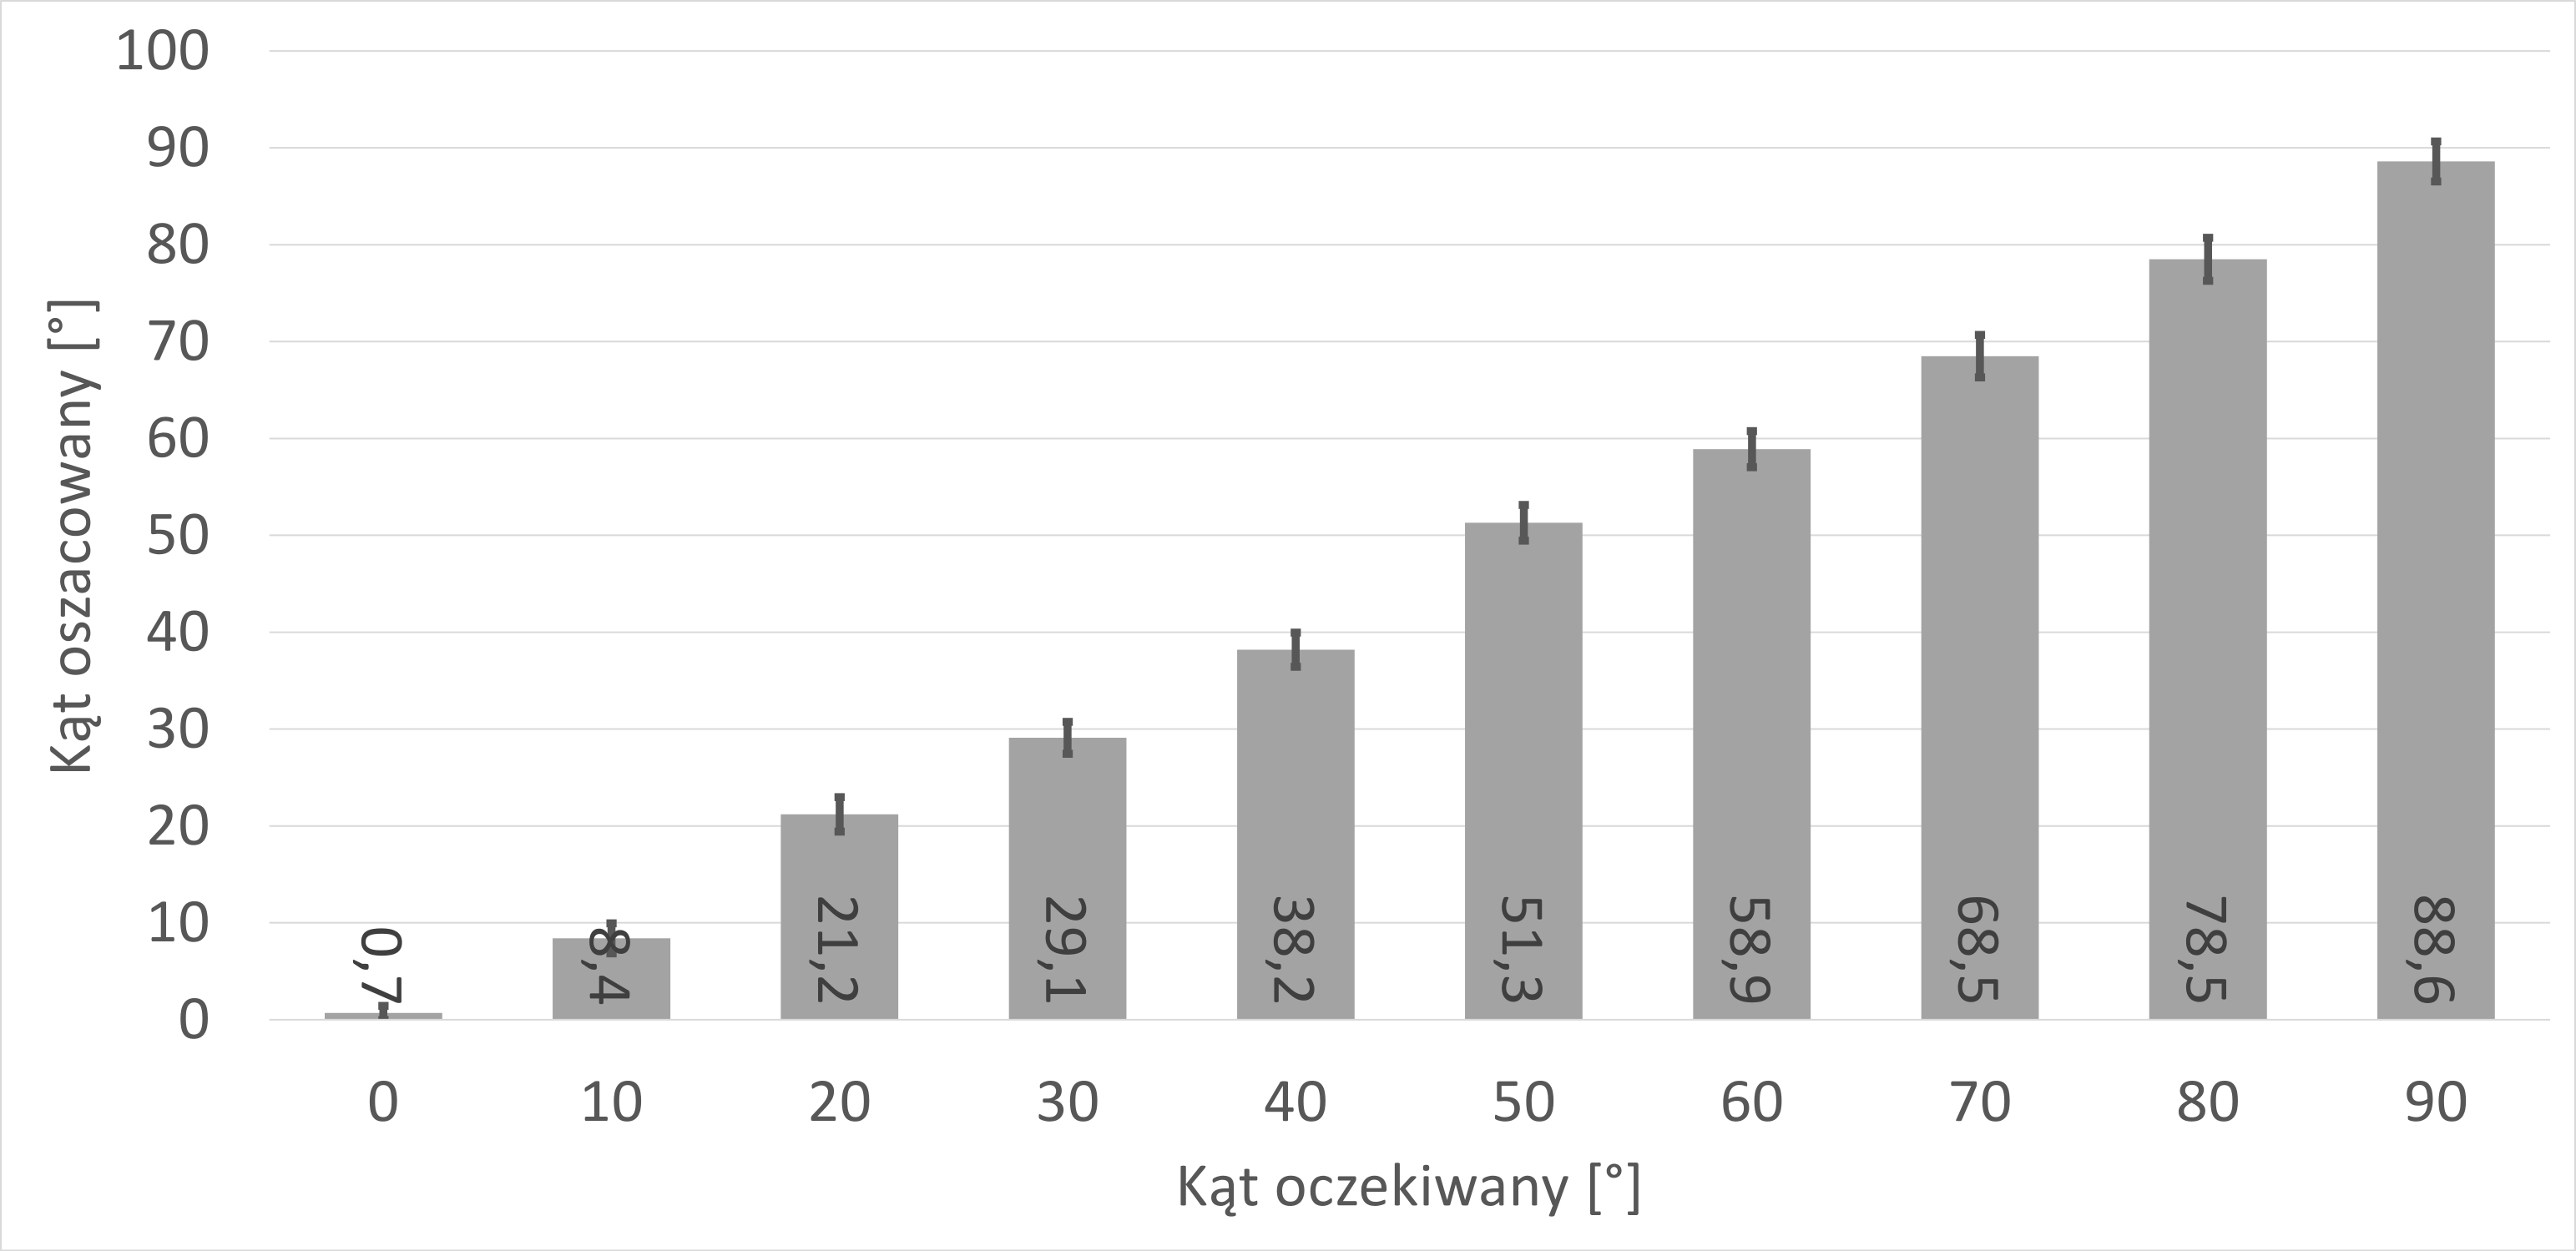
\includegraphics[width=\textwidth]{images/imumeasuredAngles.png}
		\caption{Wykres przedstawiający uśrednione wartości oszacowania kąta obrotu wokół osi $X$ i~$Y$ za pomocą modułu inercyjnego (źródło: badania własne)}
		\label{fig:hybrid:imu:XYRot}
	\end{figure}
\end{savenotes}
\begin{savenotes}
	\begin{figure}[!htb]
		\centering 
		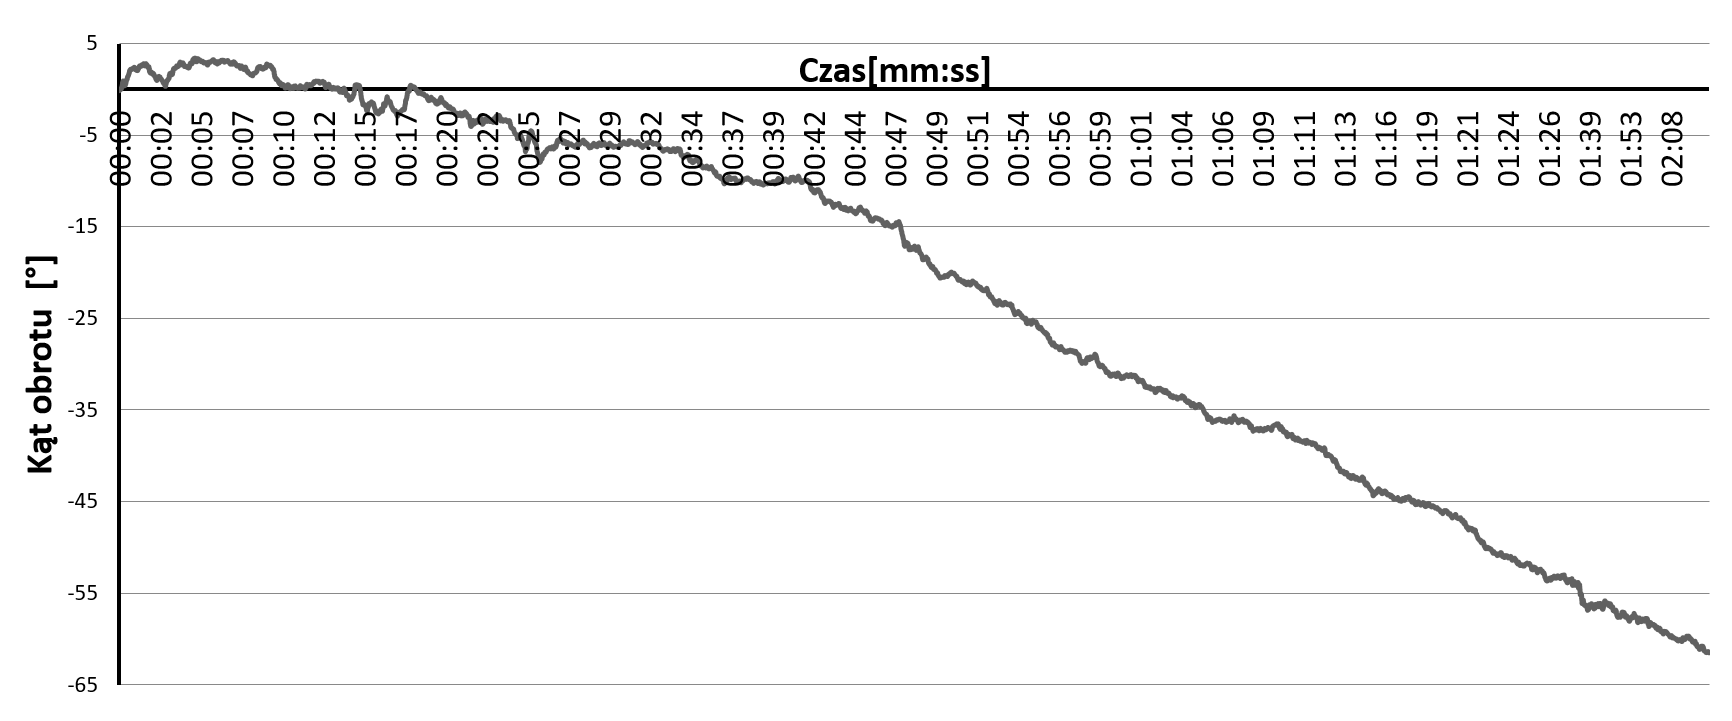
\includegraphics[width=\textwidth]{images/imuDrift.png}
		\caption{Wykres przedstawiający dryf oszacowania kąta obrotu modułu inercyjnego wokół osi $Z$ (źródło: badania własne)}
		\label{fig:hybrid:imu:drift}																														
	\end{figure}
\end{savenotes}
						
Zanim jednak dane z~akcelerometru i żyroskopu zostaną połączone ze sobą z~wykorzystaniem filtru Madgwicka, pomiary uzyskane za pomocą akcelerometru poddane są korekcie ze względu na aktualną temperaturę pracy sensora.
\begin{equation}
	A' = \frac{A}{1+f_T (T-T_0)}
	\label{eq:hybrid:temperatureCorrection}
\end{equation}

Wzór \ref{eq:hybrid:temperatureCorrection} przedstawia sposób korekty pomiaru z~akcelerometru $A$ w~określonej temperaturze $T$. Temperatura $T_0$ to temperatura neutralna, która według specyfikacji wykorzystanego układu elektronicznego oraz na podstawie własnych badań dotyczących wpływu temperatury na dokładność pomiarów czujników inercyjnych, wynosi $25\degree C$ (wykres na rys. \ref{fig:characteristics:imu:temp}). W~znanej mnie literaturze przedmiotu, korekta taka nie była uwzględniania lub autorzy tych publikacji nie zamieścili stosownej informacji o~tym fakcie.
						
Również dane dotyczące położenia w~przestrzeni wybranych stawów szkieletu, pobrane z~kontrolera Kinect, muszą zostać poddane filtracji. Umożliwia to zmniejszenie efektu ''drgania'' położenia stawów, których ruch jest śledzony oraz eliminuje krótkotrwałe zaburzenia śledzenia mające swój efekt w~postaci znaczących różnic w~położeniu danego stawu pomiędzy dwoma kolejnymi pomiarami. Na przykład przy częstotliwości pracy kontrolera Kinect wynoszącej 30 Hz przemieszczenie się stawu o~kilkanaście centymetrów, pomiędzy dwoma kolejnymi oszacowaniami, może wskazywać błąd wyznaczania pozycji lub błąd pomiaru. Aby ograniczyć wpływ opisanych szumów na dalsze etapy działania opracowanej przez autora hybrydowej metody śledzenia ruchu, pozycje wybranych stawów, których ruch jest śledzony, zostały poddane filtracji dolnoprzepustowej za pomocą filtru wykładniczego I-go rzędu. Jego działanie opiera się na komplementarnym łączeniu ze sobą zaszumionych danych dotyczących pozycji $P$ stawu $j$ pobranych z kontrolera Kinect w~chwili $t$ ($P^K_{j,t}$) z~wynikiem działania filtra w~chwili $t-1$ ($P'^K_{j,t-1}$) przy zastosowaniu współczynnika filtracji $f_{LPF}$ zgodnie ze wzorem \ref{eq:hybrid:kinect:lpf}.

\begin{equation}
	\label{eq:hybrid:kinect:lpf}
	P'^K_{j,t} = f_{LPF} P^K_{j,t} + (1-f_{LPF})P'^K_{j,t-1}
\end{equation}

Przykład danych dotyczący położenia stawu łokciowego przed i~po zastosowaniu omówionego filtra wykładniczego I-go rzędu, przedstawiają wykresy z rysunków \ref{fig:hybrid:kinect:noised} oraz \ref{fig:hybrid:kinect:denoised}.
						
	
\begin{savenotes}
	\begin{figure}[!htb]
		\centering
		\begin{subfigure}[b]{\textwidth}
			\centering
			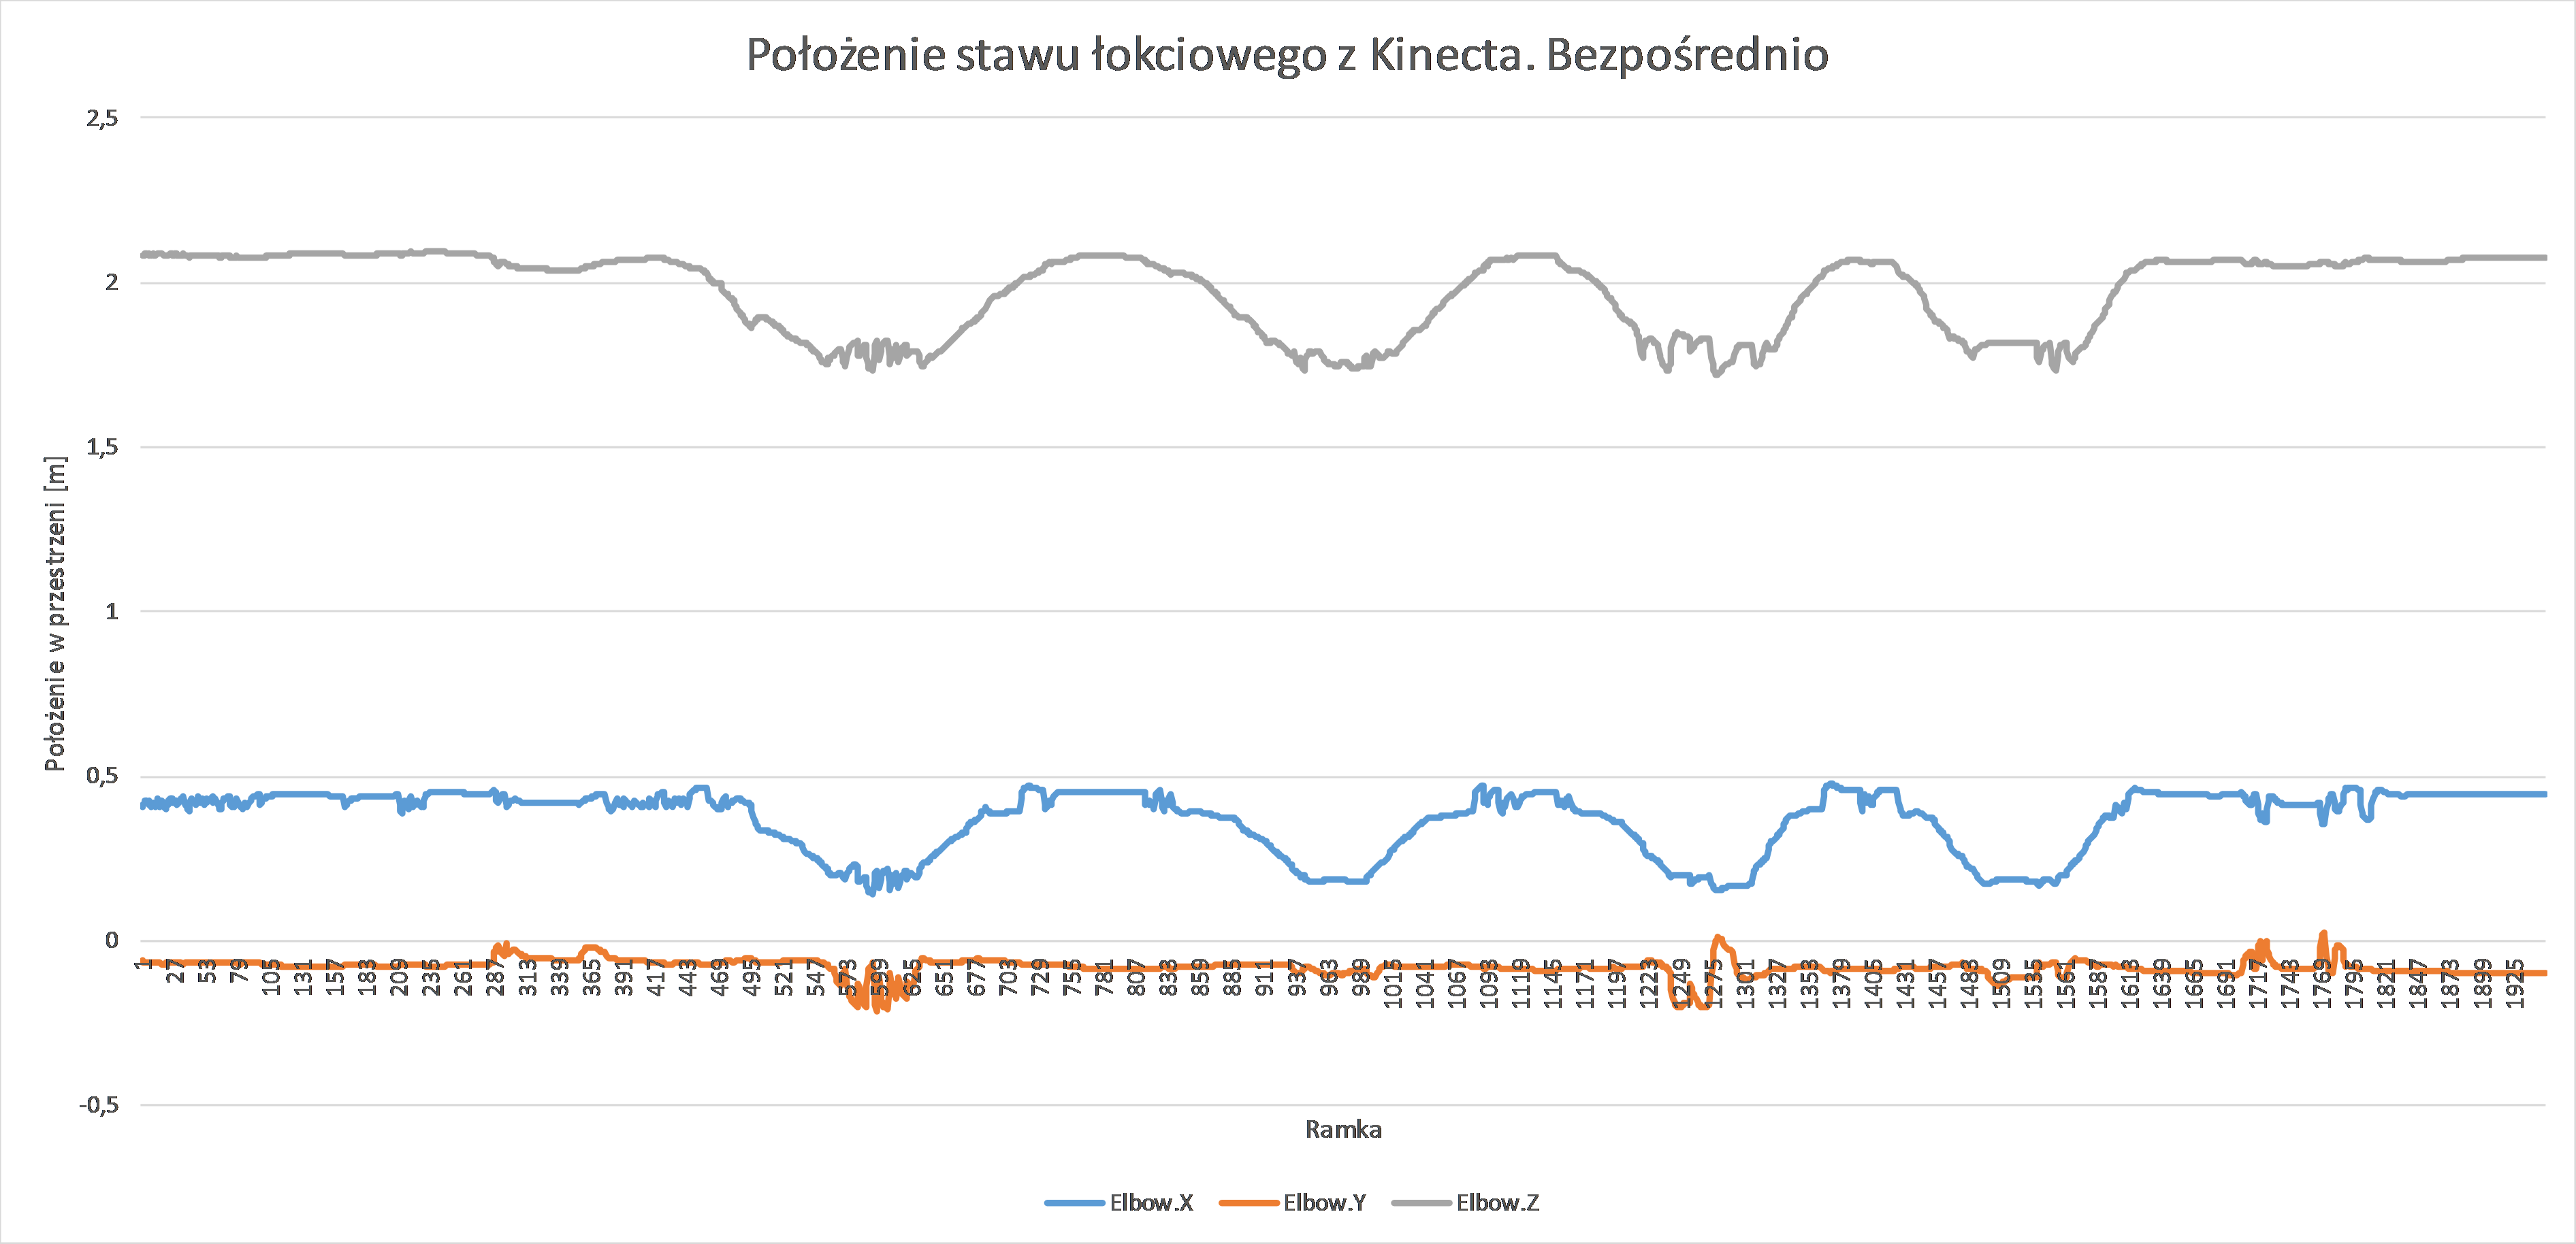
\includegraphics[width=\textwidth]{images/kinectElbowRaw.png}	
			\caption{Pomiar bezpośredni -- zaszumiony}
			\label{fig:hybrid:kinect:noised}
		\end{subfigure}
		\begin{subfigure}[b]{\textwidth}
			\centering
			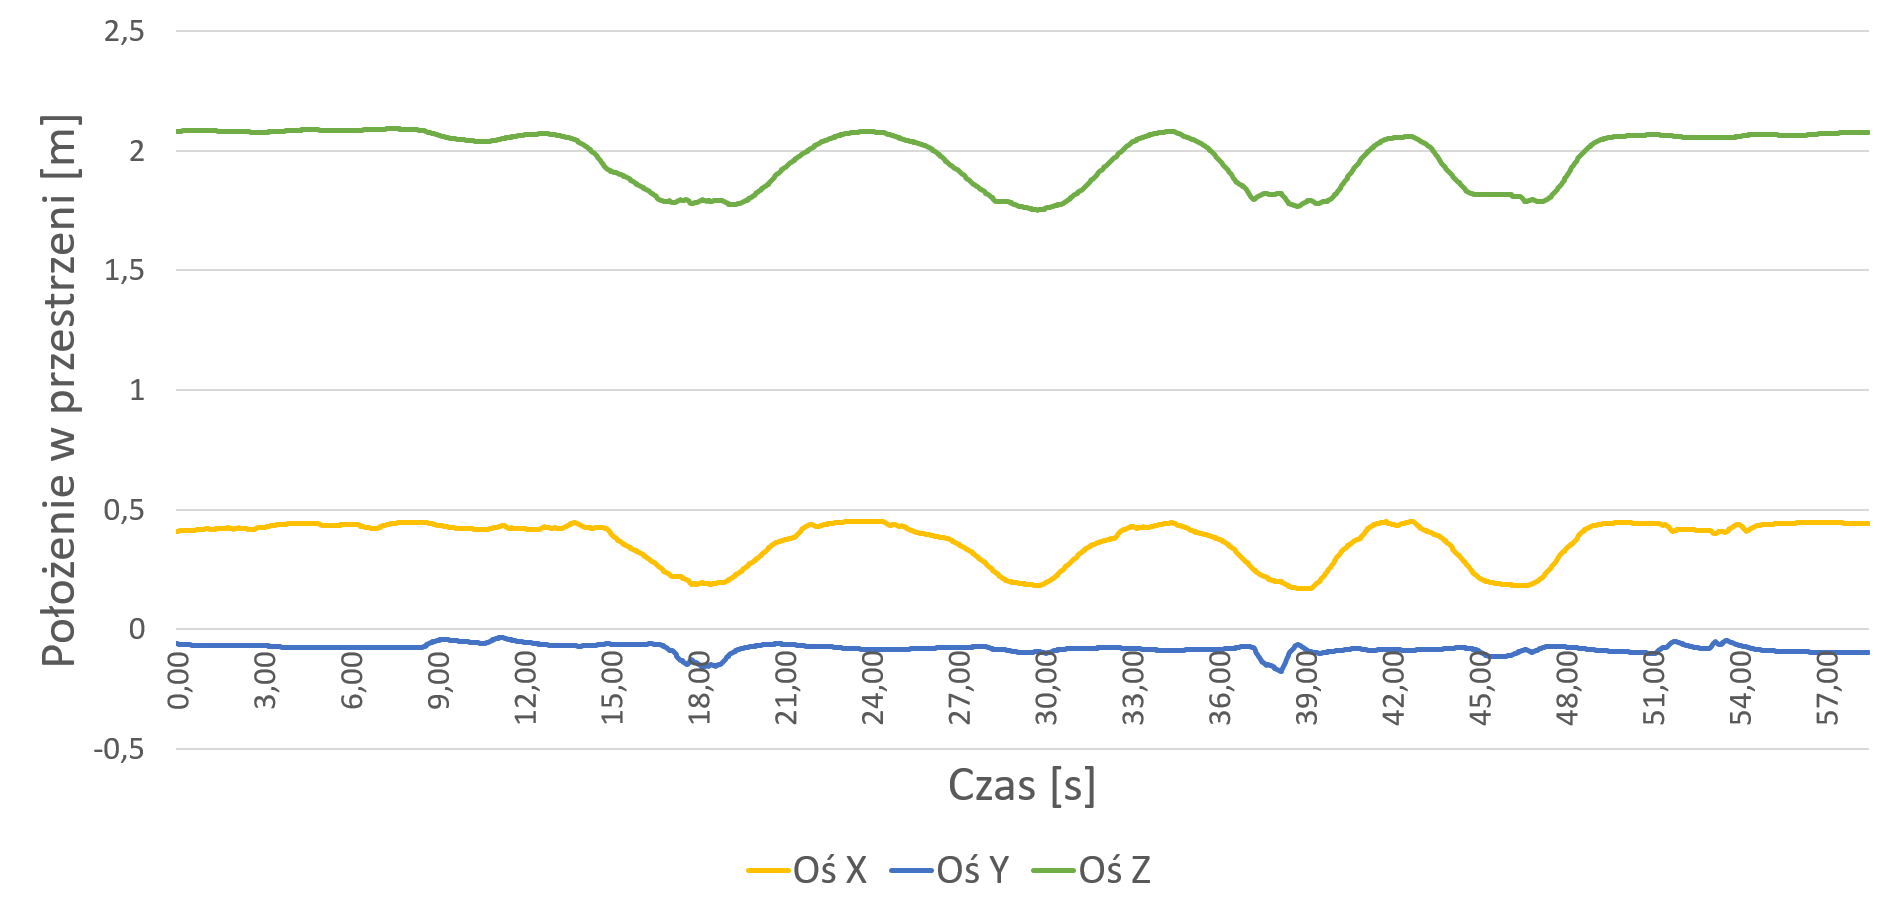
\includegraphics[width=\textwidth]{images/kinectElbowFiltered.png}	
			\caption{Pomiar odszumiony}
			\label{fig:hybrid:kinect:denoised}
		\end{subfigure}				
		\caption[Wykres przedstawiający oszacowanie położenia stawu łokciowego za pomocą kontrolera Kinect na podstawie sygnału zaszumionego oraz odszumionego]{Wykres przedstawiający oszacowanie położenia stawu łokciowego za pomocą kontrolera Kinect na podstawie sygnału zaszumionego (a) oraz odszumionego (b) filtrem wyrażonym wzorem \ref{eq:hybrid:kinect:lpf} (źródło: badania własne)}
	\end{figure}
\end{savenotes}
								
Wartość współczynnika filtracji $f_{LPF}$ została wyznaczona w~drodze prowadzonych badań własnych i~została ustalona na $0.065$. Przeprowadzone przeze mnie badanie wpływu wartości współczynnika filtracji na dokładność oszacowania pozycji stawów, za pomocą kontrolera Kinect, polegało na wyznaczeniu średniego błędu oszacowania pozycji stawów między wskazaniami kontrolera Kinect, a~danymi referencyjnymi uzyskanymi z~systemu śledzenia ruchu firmy Vicon. W~trakcie badania były wykonywane ruchy samych kończyn jak i~całego ciała, śledzone równocześnie przez system Vicon jak i~kontroler Kinect. Następnie wyznaczany był średni błąd oszacowania pozycji dla wybranych stawów, z~wykorzystaniem filtra oraz bez niego, a~także z~różnymi wartościami współczynnika $f_{LPF}$. Rysunek \ref{fig:hybrid:kinect:lpf} przedstawia wykres zależności uzyskanego średniego błędu oszacowania pozycji stawów w~zależności od wartości współczynnika filtracji $f_{LPF}$. 
								
\begin{savenotes}
	\begin{figure}[!htb]
		\centering 
		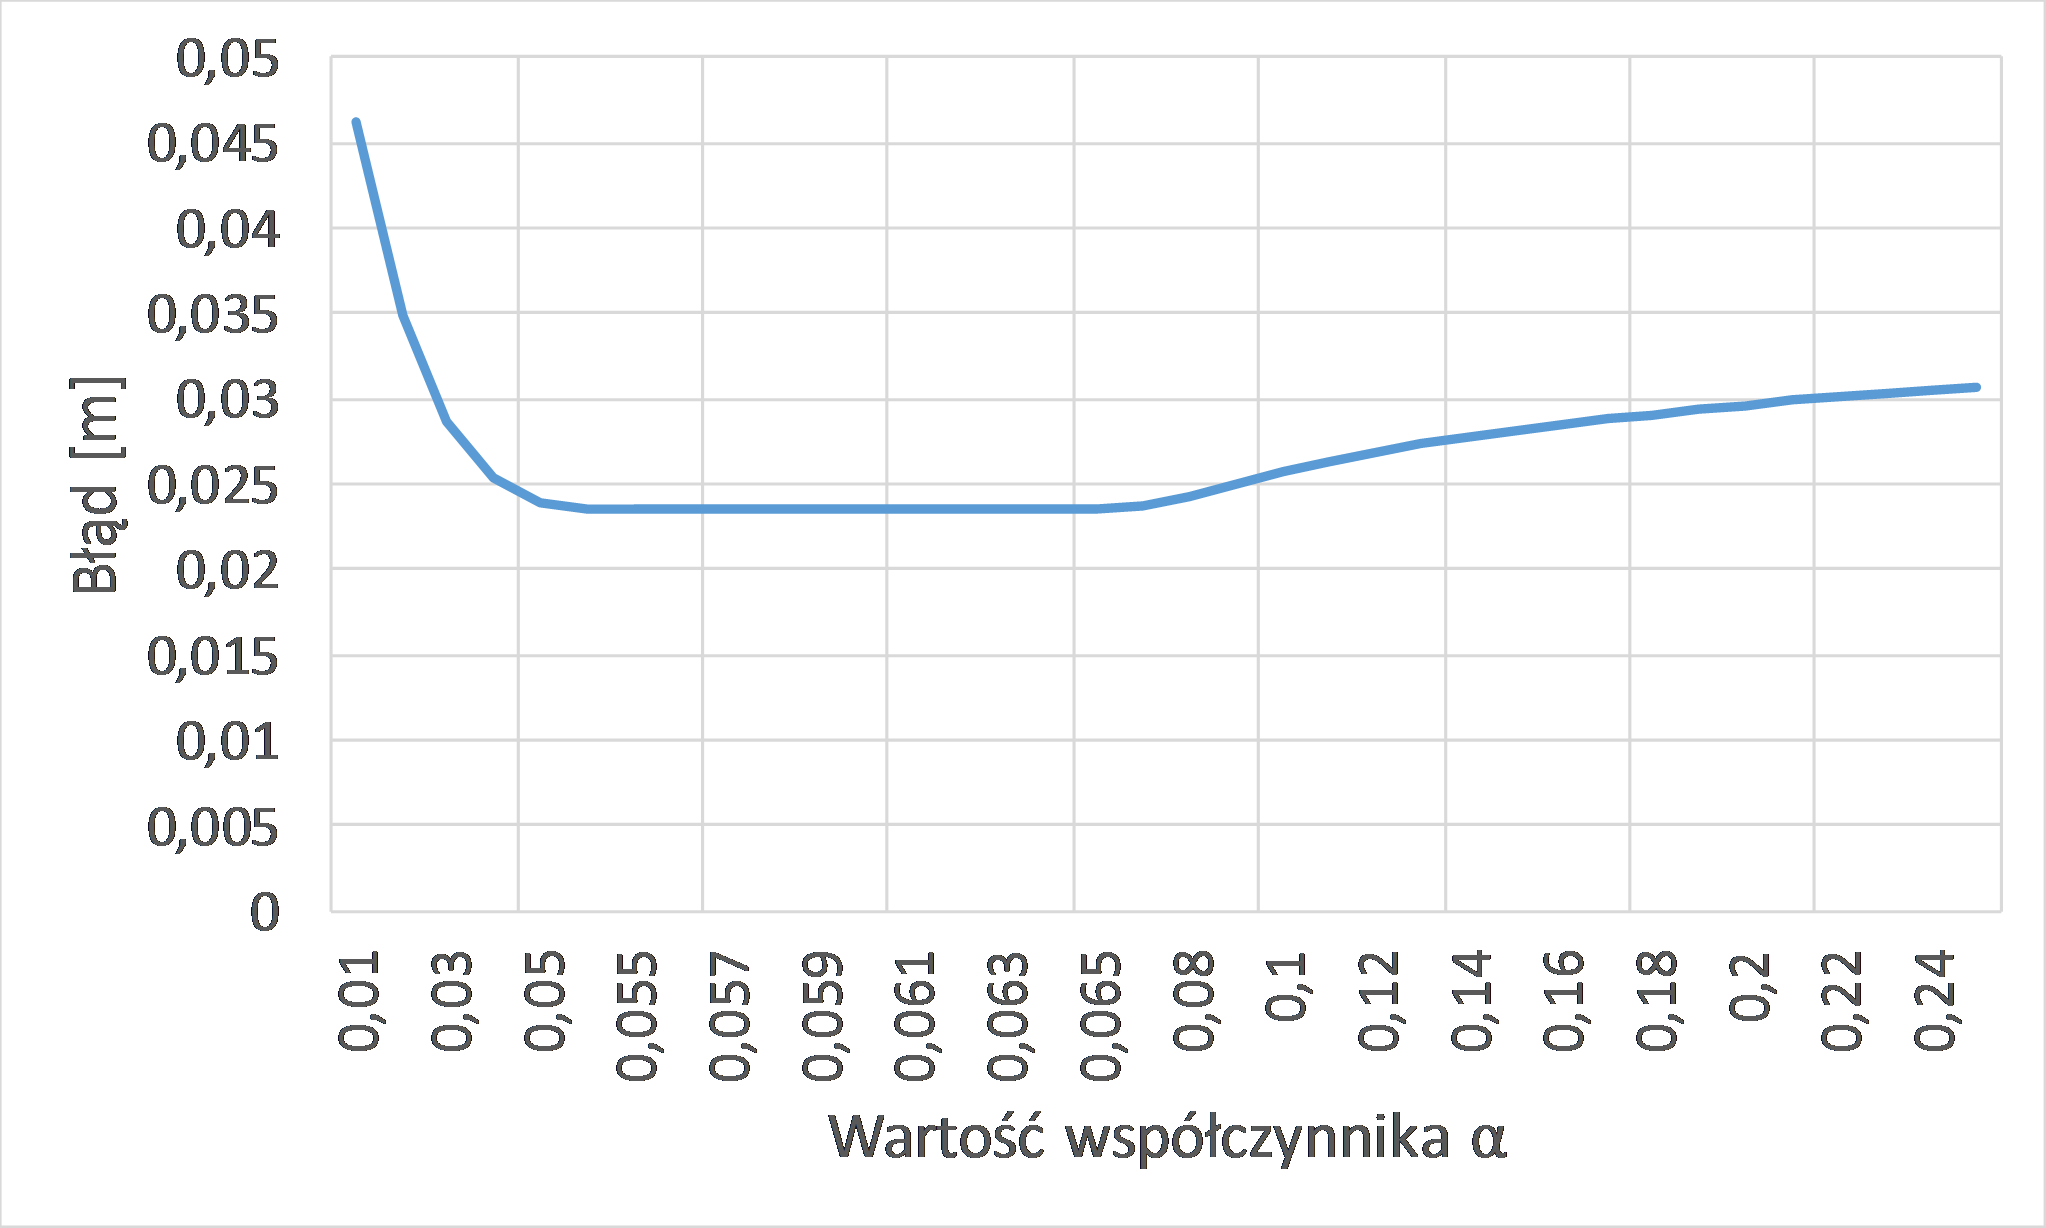
\includegraphics[width=0.75\textwidth]{images/kinectPosErrorAlpha.png}
		\caption{Wykres przedstawiający średni błąd pozycjonowania stawów za pomocą kontrolera Kinect w~zależności od współczynnika filtracji $\alpha$ (źródło: badania własne)}
		\label{fig:hybrid:kinect:lpf}
	\end{figure}
\end{savenotes}
										
Korekcie muszą zostać poddane także oszacowania odległości od kontrolera Kinect, w~jakiej znajdują się wybrane stawy. Krok ten nie był uwzględniany w dotychczas opublikowanej, znanej autorowi literaturze, a ze względu na zauważalną różnicę pomiędzy oszacowaniami Kinecta a rzeczywistą odległością, w jakiej stoi użytkownik, ma on wpływ na błędy w dalszych obliczeniach. Zgodnie ze wzorami \ref{eq:characteristics:kinect:distanceAccuracyPoly} i~\ref{eq:characteristics:kinect:distanceAccuracyCoef}, definiującymi model błędu szacowania odległości pomiędzy osobą, której ruch jest śledzony a~Kinectem, funkcja korygująca ten błąd przybiera postać wzoru \ref{eq:distCorr}.
\begin{equation}
	f(z) = z' = -0.02z^3 + 0.11z^2 - 0.27z + 0.25
	\label{eq:distCorr}
\end{equation}

gdzie wartość $z$ to oszacowanie odległości podlegające korekcie, a $z'$ to wartość skorygowana. Formuła korygująca oszacowanie odległości wykonane przez kontroler Kinect jest efektem własnego eksperymentu opisanego szerzej w~rozdziale \ref{sssection:distanceEstimation}.
										
\section{Synchronizacja czasowa}
										
Aby dane reprezentujące położenie badanego stawu, na podstawie czujników inercyjnych oraz kontrolera Kinect, mogły być poprawnie złączone, powinny zostać najpierw zsynchronizowane w~czasie. Jest to proces, który powinien zostać przeprowadzony przed każdą sesją śledzenia ruchu, na przykład przed konkretną sekwencją ćwiczeń do wykonania. Synchronizacja czasowa ma na celu określenie przesunięcia czasowego, jakie występuje pomiędzy oszacowaniami położenia tych samych stawów w~trakcie tego samego ruchu za pomocą każdego z~urządzeń pomiarowych osobno -- czujników inercyjnych i~kontrolera Kinect. Informacja dotycząca kroku związanego z synchronizacją sygnałów rozważanych urządzeń nie znalazła się w~żadnej ze znanych autorowi pozycji bibliograficznych dotyczących omawianego przedmiotu, co może wskazywać na jego pominięcie w procesie przetwarzania i łączenia sygnałów źródłowych. To z~kolei może skutkować powstaniem błędów na skutek łączenia nie skorelowanych ze sobą danych.\\
Do wyznaczenia przesunięcia czasowego pomiędzy sygnałem uzyskiwanym z~czujników inercyjnych ($I[t]$), a~tym z~kontrolera Kinect ($K[t]$) wykorzystany został algorytm korelacji wzajemnej (\emph{ang. cross--correlation}) określony wzorem \ref{eq:cross-cor:1}.

\begin{equation}
	(I \ast K)(\tau) = \int_{-\infty}^{+\infty}I[t]K[t+\tau]dt
	\label{eq:cross-cor:1}
\end{equation}

Parametr $\tau$ odpowiada za opóźnienie jednego sygnału względem drugiego. Aby wyznaczyć jakie jest przesunięcie czasowe ($\tau_{max}$) pomiędzy dwoma sygnałami należy znaleźć taką wartość argumentu $\tau$ dla której wartość funkcji korelacji wzajemnej pomiędzy badanymi sygnałami jest największa, co przedstawia wzór \ref{eq:cross-cor:2}.										
										
\begin{equation}
	\tau_{max}       = \underset{\tau}{argmax}((I \ast K)(\tau))
	\label{eq:cross-cor:2} 
\end{equation}

Aby można było skutecznie wyznaczyć tę wartość, oba sygnały muszą posiadać tę samą częstotliwość próbkowania. Spełnienie tego warunku uzyskano poprzez obniżenie częstotliwości próbkowania sygnału uzyskanego z~czujników inercyjnych ze 100Hz  do 30Hz, to znaczy została ona zrównana do tej, z~jaką pracuje Kinect. Pomiary z~czujników inercyjnych są tymczasowo buforowane i~gdy zostanie pobrany pakiet danych z Kinecta, pomiary z~modułów inercyjnych zgromadzone w~tymczasowym buforze zostają poddane filtrowi medianowemu, aby wyeliminować ewentualne krótkotrwałe zaburzenia pomiarów. 
										
W~znanej autorowi niniejszej dysertacji literaturze przedmiotu, korekta taka nie była uwzględniania lub autorzy tych publikacji nie zamieścili stosownej informacji o~tym fakcie.

Wyznaczona wartość przesunięcia w~czasie pomiędzy sygnałami ($\tau_{max}$) wykorzystywana jest następnie do modyfikacji wartości znacznika określającego czas odebrania danych z~modułu inercyjnego przez komputer PC. Tak zmodyfikowany znacznik czasu wykorzystywany jest do wyznaczenia pomiarów z~czujników inercyjnych odpowiadających pomiarom uzyskanym z~kontrolera Kinect. Metoda określająca odpowiadające sobie pomiary z~kilku sygnałów, na podstawie czasów otrzymania wartości każdego z~badanych sygnałów, nazywana jest decymacją \cite{Hinton2001}. Przyjmując, że $t_K$ jest znacznikiem czasowym otrzymania na komputerze PC danych z~kontrolera Kinect, a~$t_I[]$ to zbiór znaczników czasowych próbek otrzymanych z~czujników inercyjnych i~umieszczonych w~buforze, wówczas wybór próbki danych pomiarowych z~czujników inercyjnych skorelowanych z~danymi z~kontrolera Kinect wyrażony jest wzorem \ref{eq:dec}
										
\begin{equation}
	i_{res} = \underset{i}{argmin}(|t_K-(t_I[i] + \tau_{max})|)
	\label{eq:dec}
\end{equation}

gdzie $i_{res}$ to numer próbki umieszczonej w~buforze danych odpowiadającej danym otrzymanym z Kinecta ze znacznikiem czasowym $t_K$.
										
W trakcie prowadzonych autorskich prac badawczych, oprócz wyznaczenia przesunięcia czasowego pomiędzy czujnikami inercyjnymi, a~kontrolerem Kinect, zostało zbadane przesunięcie czasowe pomiędzy tymi urządzeniami pomiarowymi, a~systemem śledzenia ruchu Vicon. Przyjmując, że Vicon działa w~czasie rzeczywistym, przesunięcia te określają de facto jakie jest opóźnienie między IMU i~Kinectem, a~rzeczywistym ruchem. I~tak, średnie przesunięcie czasowe pomiędzy czujnikami inercyjnymi a~systemem Vicon wyniosło około $0.04s$, natomiast pomiędzy Kinectem a~systemem Vicon to około $0.09s$. Korelacja wyznaczona między czujnikami inercyjnymi a~kontrolerem Kinect wskazuje, że średnie przesunięcie szacowania pozycji wynosi około $0.06s$. Z uwagi na to, że dane z~czujników inercyjnych są łączone z~pomiarami uzyskanymi z~kontrolera Kinect, zgodnie z~częstotliwością pracy Kinecta, zasadnym jest wskazanie, że opisywana przez autora metoda łączenia danych ze wspomnianych urządzeń posiada opóźnienie $0.09s$ względem rzeczywistego ruchu.
										
\section{Łączenie danych}
										
Strumienie danych pochodzące z~poszczególnych sensorów, zsynchronizowane czasowo oraz poddane filtracji mogą zostać połączone celem uzyskania wypadkowych wartości, lepiej odzwierciedlających układ szkieletu śledzonej postaci. Na tym etapie prezentowana metoda opiera się na informacji o~orientacji przestrzennej poszczególnych kości zamiast na położeniu konkretnych stawów. Jest to nowe podejście do łączenia sygnałów z~czujników inercyjnych z sygnałami z~kontrolera Kinect, które stanowi jedno z~głównych osiągnięć prezentowanej pracy. Podejście takie podyktowane jest faktem, że w~przypadku czujników inercyjnych, wyznaczenie położenia stawów wymaga połączenia informacji o~orientacji przestrzennej czujników z~modelem szkieletowym zawierającym informację o~długościach poszczególnych kości. Z~uwagi, że wykorzystując definicję modelu szkieletowego, definicja długości jego segmentów jest stała, należy zwrócić szczgólną uwagę na dokładność pomiarów tych długości. Wszelkie błędy i~niedokładności popełnione na tym etapie przygotowywania modelu możne skutkować pojawieniem się istotnych błędów w~oszacowaniu położenia poszczególnych stawów. Co więcej, ze względu na hierarchiczną budowę modelu szkieletowego, ewentualne błędy wynikające z~braku dokładnych pomiarów długości poszczególnych kości szkieletu będą się kumulowały wraz z~odległością danego segmentu od korzenia. 

Wykorzystanie położenia stawów szkieletu w~procesie łączenia sygnałów z~obu źródeł, dodatkowo utrudnia fakt niedokładności w~oszacowaniu modelu szkieletowego za pomocą kontrolera Kinect. Model ten nie ma zdefiniowanych długości poszczególnych kości na stałe (choćby na czas pojedynczej sesji śledzenia) i~są one determinowane przez oszacowanie położenia kolejnych stawów, obarczonych zauważalną zmiennością w~czasie. To z~kolei skutkuje tym, że długości poszczególnych kości modelu szkieletowego, oszacowanego przez kontroler Kinect, różnią się nawet o~kilka $cm$ pomiędzy kolejnymi pomiarami.
										
Dane z~obu źródeł (kontroler Kinect i~moduł inercyjny) zawierają informacje o~orientacji przestrzennej wyrażone w~kwaternionach, jednak dalsze obliczenia, mające na celu połączenie tych informacji, są bardziej intuicyjne przy reprezentacji w~postaci kątów Eulera. Konwersja taka przeprowadzona jest zgodnie ze wzorem \ref{eq:appx:rot:quatToEuler}, a~w~jej wyniku wartości obrotów wokół każdej z~osi układu współrzędnych danego urządzenia pomiarowego, które składają się na orientację przestrzenną danej kości, są wyrażone bezpośrednio. Reprezentacja w~postaci kątów Eulera ułatwia także konwersję informacji o~obrotach do wspólnego, globalnego układu współrzędnych, co jest niezbędne, żeby można było je w~dalszych krokach łączyć. Informacje o~orientacji kości, wyznaczone na podstawie danych pomiarowych z~czujników inercyjnych oraz kontrolera Kinect, są od siebie niezależne i uzupełniają się nawzajem. Wzajemna niezależność i~uzupełnianie się danych umożliwia ich połączenie w~sposób komplementarny. Łącząc dane w~sposób komplementarny, każdej z~wartości podlegającej łączeniu przypisane zostają wagi, których suma wynosi $1$, a~następnie są one ze sobą sumowane z~uwzględnieniem wag określających poziom istotności poszczególnych wartości kątów. Wynik sumowania reprezentuje wartość złączonych danych wejściowych. \\
										
Prezentowana w~niniejszej dysertacji hybrydowa metoda śledzenia ruchu kończyn człowieka łączy ze sobą dane pochodzące z~dwóch źródeł. Dane te są w~postaci trójelementowych wektorów orientacji $E^i = \begin{bmatrix} \phi &  \theta & \psi \end{bmatrix}^i$ ($i = \{I,K\}, I-\text{IMU}; K-\text{Kinect}$), gdzie każdy z~elementów oznacza obrót wokół pojedynczej osi układu współrzędnych odpowiednio $X \quad Y \quad Z$. Wektor ten stanowi reprezentację orientacji przestrzennej segmentu szkieletu w~postaci kątów Eulera, wyznaczoną przez konwersję kwaternionów otrzymanych na podstawie pomiarów czujników inercyjnych ($E^I$) lub~kontrolera Kinect($E^K$). Wagi wykorzystywane w~procesie łączenia danych są wyznaczane indywidualnie dla każdego z~elementów wektora. Przyjmując, że wagi $w_\phi , w_\theta , w_\psi$ oznaczają poziom istotności informacji otrzymanych na podstawie pomiarów czujników inercyjnych ($E^I = \begin{bmatrix}  \phi^I &  \theta^I &  \psi^I \end{bmatrix}$), wówczas komplementarne łączenie ich z~danymi otrzymanymi z~kontrolera Kinect ($E^K = \begin{bmatrix}  \phi^K &  \theta^K &  \psi^K \end{bmatrix}$) dla danej chwili $t$ pozwala oszacować złączone kąty Eulera $E^F$ ($F$ -- złączone, \emph{ang. Fused}) według wzoru \ref{eq:hybrid:reliableFusion}
										
\begin{equation} E^F_t = 
	\begin{bmatrix}  \phi^F \\  \theta^F \\  \psi^F \end{bmatrix}_t = 
	\begin{bmatrix} w_\phi * \phi^I \\ w_\theta * \theta^I \\ w_\psi * \psi^I \end{bmatrix}_t + 
	\begin{bmatrix} (1-w_\phi) * \phi^K \\ (1-w_\theta) * \theta^K \\ (1-w_\psi) * \psi^K \end{bmatrix}_t
	\label{eq:hybrid:reliableFusion}
\end{equation}
										
Wzór \ref{eq:hybrid:reliableFusion} jest wykorzystywany zawsze wtedy, kiedy dane podlegające łączeniu są dobrej jakości i~możemy je uznać za prawidłowe. W~takiej sytuacji współczynniki wag $w_\phi , w_\theta , w_\psi$ są wartościami stałymi dobranymi eksperymentalnie przez autora i~wynoszącymi odpowiednio $0.98,0.05,0.65$.\\
Waga $w_\phi$ odpowiada za obrót wokół osi przechodzącej wzdłuż ciała (oś $X$, rys. \ref{fig:characteristics:kinect:space} i \ref{fig:handAxes}). Wysoka wartość tej wagi wynika z~faktu, że wartość obrotu wokół tej osi jest mierzalna jedynie przez czujniki inercyjne. Dzięki wadze zbliżonej do wartości $1$, pomiary uzyskane z~Kinecta są niemal ignorowane.\\
$w_\theta$ jest wagą określającą istotność informacji o~obrocie wokół osi zgodnej z~kierunkiem działania grawitacji (oś $Y$, rys. \ref{fig:characteristics:kinect:space} i \ref{fig:handAxes}). Wartość tego obrotu jest bardziej wiarygodnie i~stabilnie szacowana w~czasie przez kontroler Kinect. Niska wartość wagi $w_\theta$ zmniejsza wpływ danych wyznaczonych na podstawie pomiarów czujników inercyjnych (obarczonych znaczącym dryfem) na wartości wypadkowe będące wynikiem łączenia danych.\\ 
Waga $w_\psi$ określa poziom istotności informacji o~obrocie wokół osi skierowanej w~stronę obserwacji kontrolera Kinect (rys. \ref{fig:characteristics:kinect:space}). Obrót ten jest szacowany zarówno przez kontroler Kinect jak i~na podstawie pomiarów z~czujników inercyjnych. Oszacowania te mają jednak różną dokładność i~różnica ta jest odzwierciedlona w~przyjętej empirycznie wartości wagi. Według badań opublikowanych przez twórcę filtru Madgwicka \cite{Madgwick2010}, wykorzystywanego w~niniejszej pracy, jego metoda wyznaczania orientacji przestrzennej, na podstawie pomiarów z~czujników inercyjnych, zapewnia dokładność około $\pm2\degree$. W~badaniach własnych autora dokładność ta była zbliżona do $\pm3\degree$. Z kolei dokładność oszacowania obrotu wokół osi $Z$ kontrolera Kinect (rys. \ref{fig:characteristics:kinect:space}, rys. \ref{fig:handAxes}) przez to właśnie urządzenie, określona na podstawie badań własnych jak i~opisów dostępnych w~literaturze \cite{Huber2015}, wynosi około $\pm6\degree$. Niemal dwukrotnie mniejszy błąd oszacowania obrotu wokół osi $Z$, na podstawie pomiarów z~czujników inercyjnych, ma swoje przełożenie na wartość wagi $w_\psi$.\\
Rysunek \ref{fig:handAxes} przedstawia układ współrzędnych wraz z~obrotami odpowiadającymi każdej z~osi tego układu, w~odniesieniu do ręki człowieka.
										
\begin{savenotes}
	\begin{figure}[!htb]
		\centering	
		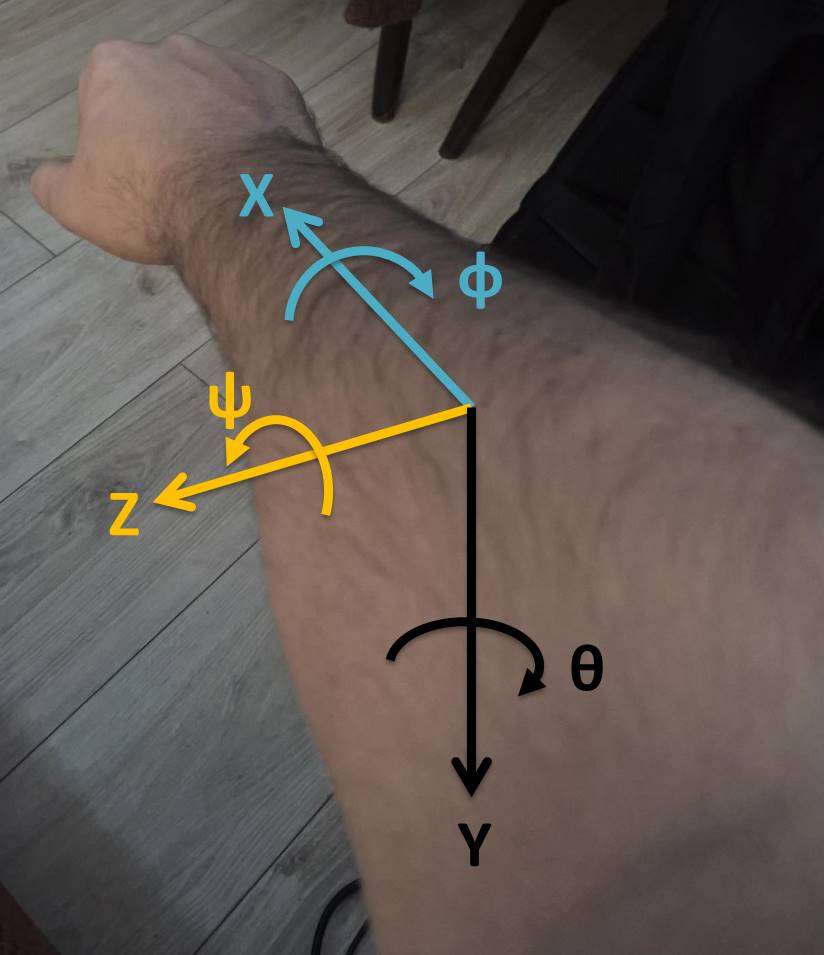
\includegraphics[width=0.6\textwidth]{images/handAxes.jpg}	
		\caption{Odniesienie układu współrzędnych $XYZ$ wraz z~obrotami $\phi , \theta , \psi$ w stosunku do ręki człowieka (źródło: opracowanie własne)}
		\label{fig:handAxes}
	\end{figure}
\end{savenotes}
												
Określenie czy oszacowania kątów, uzyskane za pomocą kontrolera Kinect, są wystarczającej jakości do łączenia ich z~oszacowaniami kątów uzyskanymi z~czujników inercyjnych, wykonywane jest każdorazowo na podstawie kryteriów związanych z~realizowanym ruchem. \\
Pierwszym kryterium branym pod uwagę jest obrót całej sylwetki względem kamery, liczony jako kąt $\alpha$ pomiędzy linią barków a~kamerą w~płaszczyźnie $X$--$Z$ (rys. \ref{fig:characteristics:kinect:bodyRotationAngle}) zgodnie ze wzorem \ref{eq:characteristics:kinect:bodyRotationAngle}. Na podstawie zbadanych wcześniej charakterystyk obu urządzeń wiadomo, że dane które można wiarygodnie wykorzystać do łączenia są możliwe do uzyskania tylko gdy sylwetka nie jest obrócona o~więcej niż $50\degree$. Oprócz wartości kąta obrotu sylwetki brane jest także pod uwagę odchylenie standardowe estymacji tego obrotu. Przyjmując, że $\alpha[]$ to zbiór wartości oszacowań kąta obrotu sylwetki z~ostatnich $3s$ (ok. 90 elementów w~zbiorze), a~$\overline{\alpha}$ to średnia arytmetyczna elementów w~tym zbiorze, wówczas odchylenie standardowe $\sigma_\alpha$ definiuje wzór \ref{eq:stdDev}.
												
\begin{equation}
	\sigma_\alpha = \sqrt{\frac{1}{n}\sum_{i=1}^{n}{(\alpha[i] - \overline{\alpha})^2}}
	\label{eq:stdDev}
\end{equation}
												
Branie pod uwagę zarówno wartości estymacji obrotu sylwetki wraz z~odchyleniem standardowym uzyskiwanych oszacowań spowodowane jest faktem, że w~momencie wystąpienia okluzji jednego lub obu stawów barkowych i~błędów oszacowania ich położenia, następuje błędne oszacowanie wartości obrotu. W~praktyce oznacza to, że wyznaczony kąt obrotu sylwetki może przyjąć dowolną wartość. Przykład szacowania kąta obrotu sylwetki względem kontrolera Kinect przedstawia wykres z rysunku \ref{fig:hybrid:kinect:kinectRotationVariance}. W~trakcie tego eksperymentu badawczego wykonywany był obrót postaci względem kontrolera Kinect do kąta $90\degree$ i~powrót do pozycji równoległej do urządzenia pomiarowego, czyli do kąta $0\degree$. Przy obrocie sylwetki nie przekraczającym $50\degree$ odchylenie standardowe oszacowań z~przyjętego okresu czasu nie przekraczało wartości $1.5\degree$. W~związku z~tym w~opisywanej w~niniejszej dysertacji hybrydowej metodzie śledzenia ruchu kończyn człowieka, autor przyjął, że pomiar obrotu postaci w~stosunku do kontrolera Kinect jest wiarygodny, jeśli oszacowanie jego kąta obrotu jest $\alpha \le 50\degree$ przy odchyleniu standardowym $\sigma_\alpha\le 1.5 \degree$.
												
\begin{savenotes}
	\begin{figure}[!htb]
		\centering
		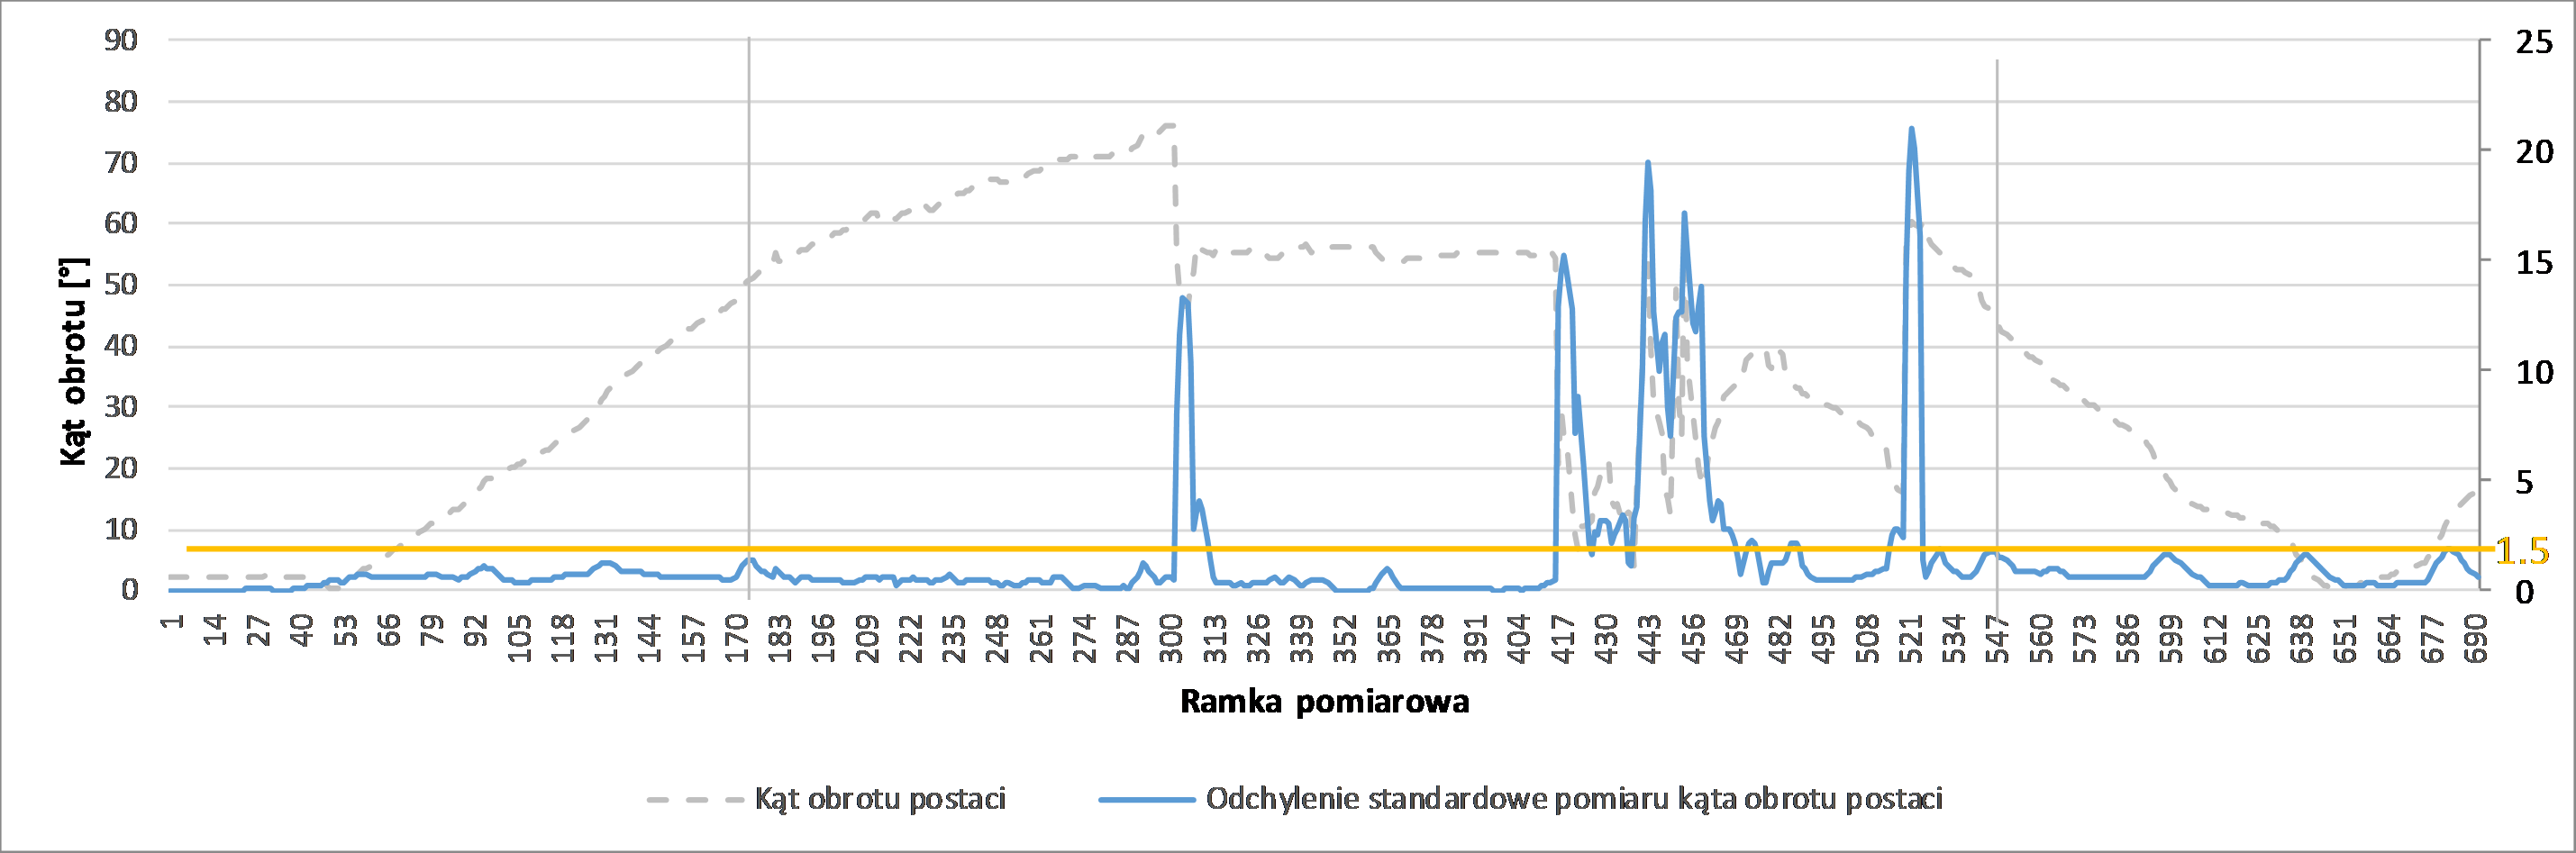
\includegraphics[width=\textwidth]{images/kinectRotationStdDev.png}
		\caption{Odchylenie standardowe estymacji kąta obrotu postaci względem Kinecta  (źródło: badania własne)}						
		\label{fig:hybrid:kinect:kinectRotationVariance}
	\end{figure}
\end{savenotes}
														
Oprócz obrotu całej postaci, ocenie podlega także stabilność pomiarów samych stawów. Pierwszym parametrem, jaki brany jest pod uwagę, jest stan śledzenia poszczególnych stawów, który może przyjąć jedną z~trzech wartości opisanych szerzej w~podrozdziale \ref{ssec:characteristics:kinect:limitation}. Wartość \emph{NotTracked} jest od razu traktowana jako wskazanie, że dane związane z~danym stawem (jego pozycja, ale także orientacja kości z~nim związanych) są niewiarygodne. W~przypadku pozostałych dwóch możliwych stanów śledzenia stawu, sprawdzany jest poziom szumu za pomocą filtru górnoprzepustowego w~postaci wzoru \ref{eq:hybrid:kinect:hpf}. 
														
\begin{equation}
	n^K_{j,t} = f_{HPF} * (n^K_{j,t-1} + P^K_{j,t} - P^K_{j,t-1}) 
	\label{eq:hybrid:kinect:hpf}
\end{equation}
														
gdzie: $n^K_{j,t}$ to poziom szumu $n$ w~aktualnym oszacowaniu położenia danego stawu $j$ w czasie $t$ dla Kinecta, $n^K_{j,t-1}$ -- poziom szumu $n$ w~poprzednim oszacowaniu położenia danego stawu $j$ w czasie $t-1$ dla Kinecta,	$P^K_{j,t}$ jest położeniem $P$ stawu $j$ w~aktualnym oszacowaniu $t$ dla Kinecta, $P^K_{j,t-1}$ to położenie  $P$ stawu $j$ w~poprzednim oszacowaniu $t-1$ dla Kinecta, natomiast $f_{HPF}$ jest współczynnikiem filtracji  $f_{HPF} = 0.01$. 
												
\begin{savenotes}
	\begin{figure}[!htb]
		\centering 
		\begin{subfigure}[b]{\textwidth}
			\centering
			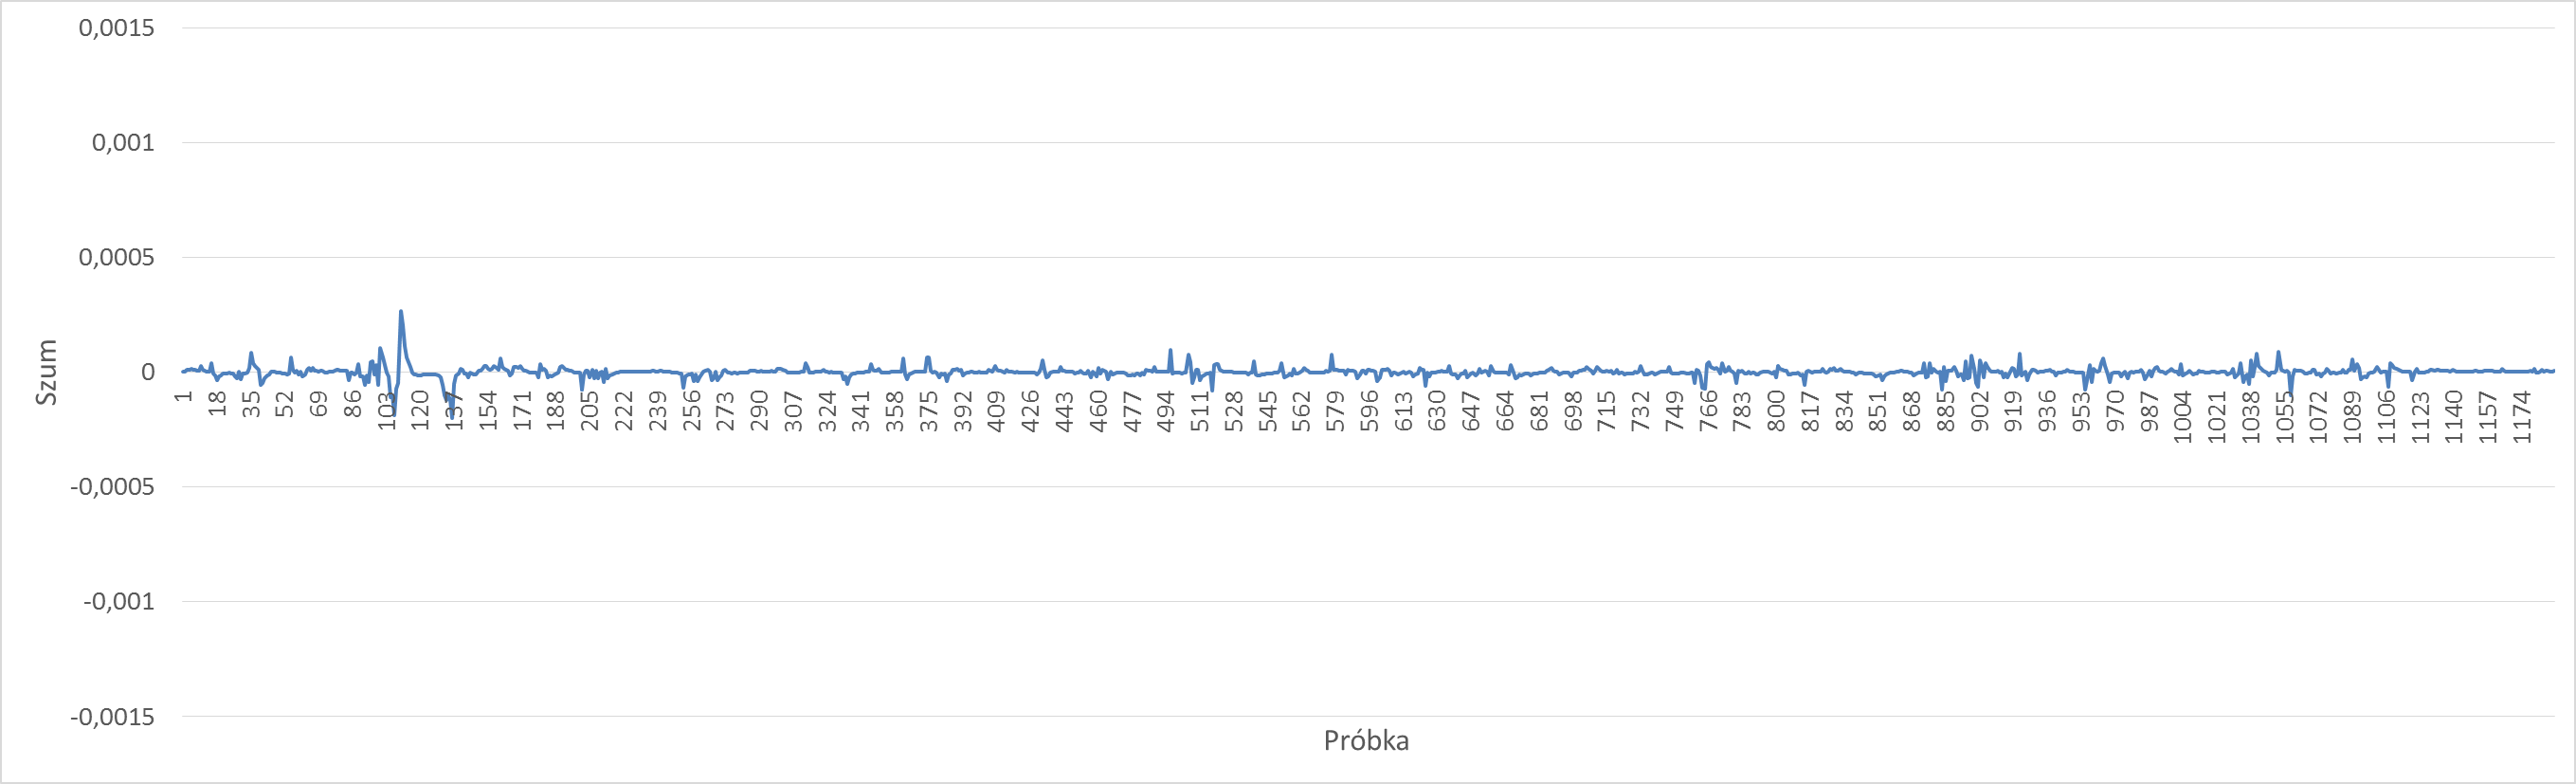
\includegraphics[width=\textwidth]{images/Fig09.png}	
			\caption{Staw śledzony ze statusem \emph{Tracked}}
			\label{fig:hybrid:kinect:hpfNotOccluded}
		\end{subfigure}	
																																									
		\begin{subfigure}[b]{\textwidth}
			\centering
			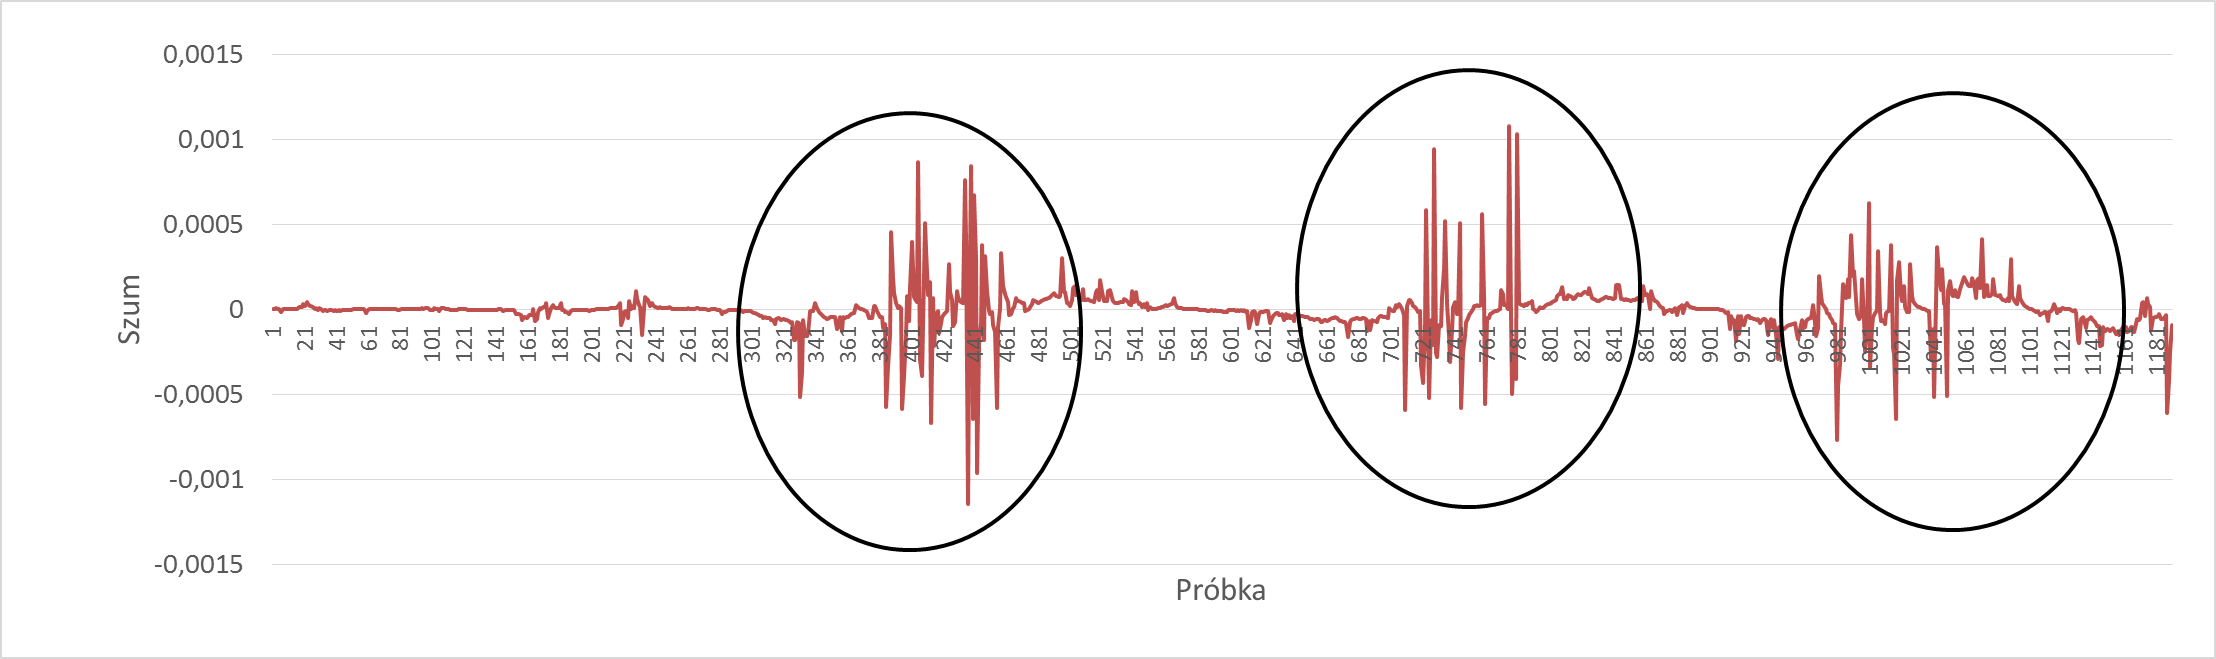
\includegraphics[width=\textwidth]{images/Fig10.png}
			\caption[Staw śledzony ze statusami \emph{Tracked} i~\emph{Interferred}]{Staw śledzony ze statusami \emph{Tracked} i~\emph{Interferred} (oznaczone owalem)}
			\label{fig:hybrid:kinect:hpfOccluded}
		\end{subfigure}	
		\caption[Wykres wartości szumu w oszacowaniach kontrolera Kinect]{Wykres wartości szumu występującego w~oszacowaniach do położenia wybranych stawów w~przestrzeni w~osi $Z$ dla stawu śledzonego ze stałym statusem \emph{Tracked} (a) oraz zmiennym statusem \emph{Tracked} i~\emph{Interferred} (b)  (źródło: badania własne)}
		\label{fig:hybrid:kinect:hpfResults}
	\end{figure}
\end{savenotes}
																
Wykresy z rysunków \ref{fig:hybrid:kinect:hpfNotOccluded} i~\ref{fig:hybrid:kinect:hpfOccluded} przedstawiają wynik działania filtru górnoprzepustowego dla oszacowania położenia stawu nadgarstkowego w~przypadku kiedy staw cały czas posiadał status śledzenia \emph{Tracked} oraz kiedy w~trakcie wykonywanego ruchu status zmieniał się na \emph{Interferred}. Dla zachowania przejrzystości, wykresy przedstawiają wspomniany wynik dla położenia stawu wyznaczonego wzdłuż jednej z~osi. Na wykresie z rysunku \ref{fig:hybrid:kinect:hpfOccluded} zostały zaznaczone owalami te miejsca, w~których nastąpiła zmiana statusu śledzenia. Na wspomnianych wykresach widać, że poziom szumu pozostaje niski dla oszacowania położenia stawu, kiedy status jego śledzenia przyjmuje wartość \emph{Tracked}. W~innym przypadku poziom szumu wzrasta wielokrotnie i~utrzymuje się do momentu ponownego przyjęcia statusu  \emph{Tracked}. Zauważyć można wówczas częste zmiany oszacowania pozycji danego stawu przez kontroler Kinect, co wiąże się z widocznym efektem drgania. Na podstawie przeprowadzonych badań własnych, w~metodzie śledzenia ruchu, jako graniczną wartość zaszumienia danych pomiarowych kontrolera Kinect ($n^K$), dla których możliwe jest ich łączenie z~danymi uzyskanymi z~czujników inercyjnych na podstawie wzoru \ref{eq:hybrid:reliableFusion}, autor przyjął $|n^K| \le 0.0004$.\\
																
W przypadku, kiedy położenie stawów, wyznaczone przez kontroler Kinect, nie może być uznane za wiarygodne (zazwyczaj spowodowane jest to okluzją), równanie \ref{eq:hybrid:reliableFusion} ulega modyfikacji i~przyjmuje postać jak w~równaniu \ref{eq:hybrid:unreliableFusion}: 
																
\begin{equation} 
	\label{eq:hybrid:unreliableFusion}
	E^F_t = 
	\begin{bmatrix}  \phi^F \\  \theta^F \\  \psi^F \end{bmatrix}_t = 
	\begin{bmatrix}  \phi^F \\  \theta^F \\  \psi^F \end{bmatrix}_{t-1} +
	diag(w_\phi,w_\theta,w_\psi)
	(\begin{bmatrix}  \phi^I \\  \theta^I \\  \psi^I \end{bmatrix}_t -
	\begin{bmatrix}  \phi^I \\  \theta^I \\  \psi^I \end{bmatrix}_{t-1})
\end{equation}
																
																
W tym przypadku zmianie ulegają wartości części wag, z~jakimi zostają połączone dane. O ile wartość $w_\phi$ nie ulega zmianie i~wynosi $0.98$, o~tyle pozostałe dwie wagi są zależne od czasu i~wyrażają się wzorem \ref{eq:dynamicWeight}:
\begin{equation}
	w_{\theta} = w_{\psi} = f(t_{szum}) = (1-\frac{t_{szum}}{10}) * 0.65
	\label{eq:dynamicWeight}
\end{equation}
																
Wartość $t_{szum}$ oznacza czas trwania okresu niepewności pomiarów wyrażony w sekundach. Jeśli czas, w~którym utrzymuje się niepewność pomiarów kontrolera Kinect, przekracza $10s$ wówczas wartość $t_{szum}$ pozostaje przy wartości $10$. Maksymalny czas kiedy szacowanie położenia stawów może odbywać się na podstawie tylko na podstawie modułów inercyjnych uzależniony jest od stabilości ich pomiarów w czasie i tego jaki jest maksymalny dopuszczony błąd szacowania położenia stawów dla projektowanego systemu. Jako przykład może tutaj posłużyć dryf pomiarów jaki występuje przy szacowaniu obrotu wokół osi równoległej do wektora grawitacji (kąt $\theta$). Jeśli dryf ten wynosi około $0.5^\degree/_s$ dla wykorzystanych modułów inercyjnych wówczas w ciągu $10s$ musimy liczyć się z błędem szacowania obrotu dochodzącym do $5\degree$ co przekłada się na błąd szacowania pozycji stawu dochodzący do $2.5cm$ dla kości o długości $30cm$. Wobec uzyskiwanych dokładności szacowania pozycji stawów w~systemach śledzenia łączących dane z Kinecta z danymi z czujników inercyjnych, które wynoszą $2.5-3cm$ oznaczałoby to dwukrotny spadek dokładności szacowania w ciągu $10s$. W związku z tym, w zaproponowanej metodzie, po utracie możliwości łączenia danych z obu źródeł, szacunkowa pozycja stawu jest aktualizowania właśnie przez $10s$. Po tym czasie musi nastąpić możliwość korekty oszacowania położenia stawów na podstawie danych z obu urządzeń. W przeciwnym razie użytkownik mógłby być wprowadzany w błąd. 
											
\begin{savenotes}
	\begin{figure}[hbp]
		\centering
		\begin{tikzpicture}[
				auto,
				block/.style    = { rectangle, draw=blue, thick, 
					fill=white, text width=50, text centered,
					minimum height=2em, font=\tiny },
				newBlock/.style    = { rectangle, draw=green, thick, 
					fill=green!20, text width=55, text centered,
					minimum height=2em, font=\tiny }
			]
																													
			\node[block](IMU)at (-1,2){Czujniki inercyjne};
			\node[newBlock](Temp) at (2,0.5){Korekta \\ względem \\ temperatury (wz. \eqref{eq:hybrid:temperatureCorrection})};
			\node[block](AHRS) at (4.5,2){Filtr \\ Madgwicka + LERP};
			\node[block](EulerImu) at (7,2){Transformacja do \\ kątów Eulera (wz. \eqref{eq:appx:rot:quatToEuler})};
			\node[newBlock](Fusion) at (7, 0){Łączenie \\ orientacji (wz. \eqref{eq:hybrid:reliableFusion} i~\eqref{eq:hybrid:unreliableFusion})};
			\node[block](EulerKinect) at (7,-2){Transformacja do \\ kątów Eulera (wz. \eqref{eq:appx:rot:quatToEuler})};
			\node[newBlock](Triage) at (7,-3.5){Ocena jakości pomiarów Kinecta};
																													
																													
			\node[newBlock](LPF) at (4.5,-3.5){Filtr \\ dolnoprzepustowy (wz. \eqref{eq:hybrid:kinect:lpf})};
			\node[newBlock](Distance) at (2,-3.5){Korekta \\ odległości (wz. \eqref{eq:distCorr})};
			\node[block](Kinect)at (-1,-3.5){Kinect};
																													
			\node[block](quat) at (11.5,0){Transformacja do \\ kwaternionu (wz. \eqref{eq:appx:rot:eulerToQuat})};
			\node[block](pos) at (11.5,-3.5){Wyznaczenie pozycji stawu};
																													
			\draw[->]  (Kinect) -- node[above,font=\tiny]{P} ++ (Distance);
			\draw[->]  (Distance) --  node[above,font=\tiny]{P'} ++(LPF);
			\draw[->]  (LPF) -- (Triage);
			\draw[->]  (Triage) -- (EulerKinect);
			\draw[->]  (EulerKinect) -- node[left,font=\tiny]{$\begin{bmatrix}  \Phi^K  \Theta^K  \Psi^K \end{bmatrix}$} ++(Fusion);
																													
																													
																													
			\draw[->]  (Fusion) -- node[above,font=\tiny]{$\begin{bmatrix}  \Phi^F  \Theta^F  \Psi^F \end{bmatrix}$} ++ (quat);
			\draw[->]  (quat) -- node[left,font=\tiny]{$Q^F$}++(pos);
			\draw[->]  (EulerImu) --  node[left,font=\tiny]{$\begin{bmatrix}  \Phi^I  \Theta^I  \Psi^I \end{bmatrix}$} ++ (Fusion);
			\draw[->]  (AHRS) --  node[above,font=\tiny]{$Q^I$} ++ (EulerImu);
			\draw[->]  (Temp) -| node[below,font=\tiny]{A'}  (AHRS);
			\draw[->]  (IMU) -- node[above,font=\tiny]{G} ++ (AHRS);
			\draw[->]  (0, 1.8) -|  node[right,font=\tiny]{T} ++ (Temp);
			\draw[->]  (IMU) |-  node[below,font=\tiny]{A}  (Temp);
			\draw[dashed, ->](quat) -- (11.5,3.0) node[above,font=\tiny]{$Q^F$} -|  (AHRS);
			\draw[->]  (pos) -- node[left,font=\tiny]{$\left[p_x^F,p_y^F,p_z^F\right]$} (11.5,-4.5);
		\end{tikzpicture}
		\caption{Diagram przedstawiający kolejne etapy działania autorskiej metody łączenia danych IMU i~Kinecta.}
																
		\label{fig:hybrid:methodDiagram}
	\end{figure}
\end{savenotes}
Poszczególne etapy metody opisanej powyżej przedstawione są na diagramie z~rysunku \ref{fig:hybrid:methodDiagram} i~odzwierciedlają kroki opisane w~niniejszym rozdziale. Kolorem zielonym zostały oznaczone etapy opisywanej metody, które stanowią autorskie dokonanie autora niniejszej pracy. Zostały one samodzielnie opracowane przez autora (wz. \eqref{eq:distCorr}, \eqref{eq:hybrid:reliableFusion}, \eqref{eq:hybrid:unreliableFusion}, kryteria określenia użyteczności danych Kinecta dla procesu łączenia ich z danymi z~czujników inercyjnych) lub po raz pierwszy, kompleksowo uwzglednione w procesie łączenia danych z kontrolera ruchu Kinect i sensorów inercyjnych (wz. \eqref{eq:hybrid:temperatureCorrection} i \eqref{eq:hybrid:kinect:lpf}).
 Elementy te miały zauważalny wpływ na jakość uzyskiwanych wyników.
%\chapter{Eksperymenty badawcze}\label{chap:experiments}
Eksperymenty badawcze wyryfikujące charakterystyki sensorów, jak również dokładności opracowanej autorsko hybrydowej metody śledzenia ruchu kończyn, zostały wykonane w~laboratorium technik multimedialnych w~Centrum Technologii Informacyjnych Politechniki Łódzkiej. Jako źródło danych referencyjnych wykorzystany został zainstalowany tam system śledzenia ruchu firmy Vicon zbudowany na bazie 10 kamer Vicon T-40S \footfullcite{footnote:ViconSpec} rejestrujących ruch markerów. System ten został skonfigurowany do działania z~częstotliwością 100 klatek na sekundę, a~dane przetwarzane były przez dedykowaną aplikację Nexus w~wersji 2.0. Dane testowe niezbędne do zweryfikowania omawianej metody zostały zgromadzone przy użyciu kontrolera Microsoft Kinect w~wersji dla konsoli XBox 360 model 1414 oraz przez urządzenie rejestrujące dane z~czujników inercyjnych zaprojektowane i~wykonane samodzielnie w~oparciu o~platformę programistyczną dla systemów wbudowanych Arduino. Szczegółowy opis przeprowadzonych eksperymentów badawczych znajduje się w~dalszej części niniejszego rozdziału.

\section{Scena}
Obszar roboczy, na którym dokonywane były pomiary ruchu, został zamknięty w~przestrzeni prostopadłościanu, obserwowanej przez kamery systemu Vicon, której obrys podstawy zbliżony był do kwadratu $4m$x$4m$. W~trakcie kalibracji systemu referencyjnego punkt początkowy $\left(0, 0, 0\right)$ został zdefiniowany w~miejscu, w~którym został umieszczony kontroler Kinect. W~trakcie trwania eksperymentu, badany użytkownik stał w~odległości ok. $2m$ od Kinecta, czyli w~odległości, w~której działa on najbardziej dokładnie.  Pełne rozmieszczenie urządzeń na scenie prezentuje rysunek \ref{fig:experiments:scene}. Prostokąty dookoła obszaru roboczego oznaczone V1 -- V10 to kamery systemu Vicon.

\begin{figure}[!htb]
	\centering
	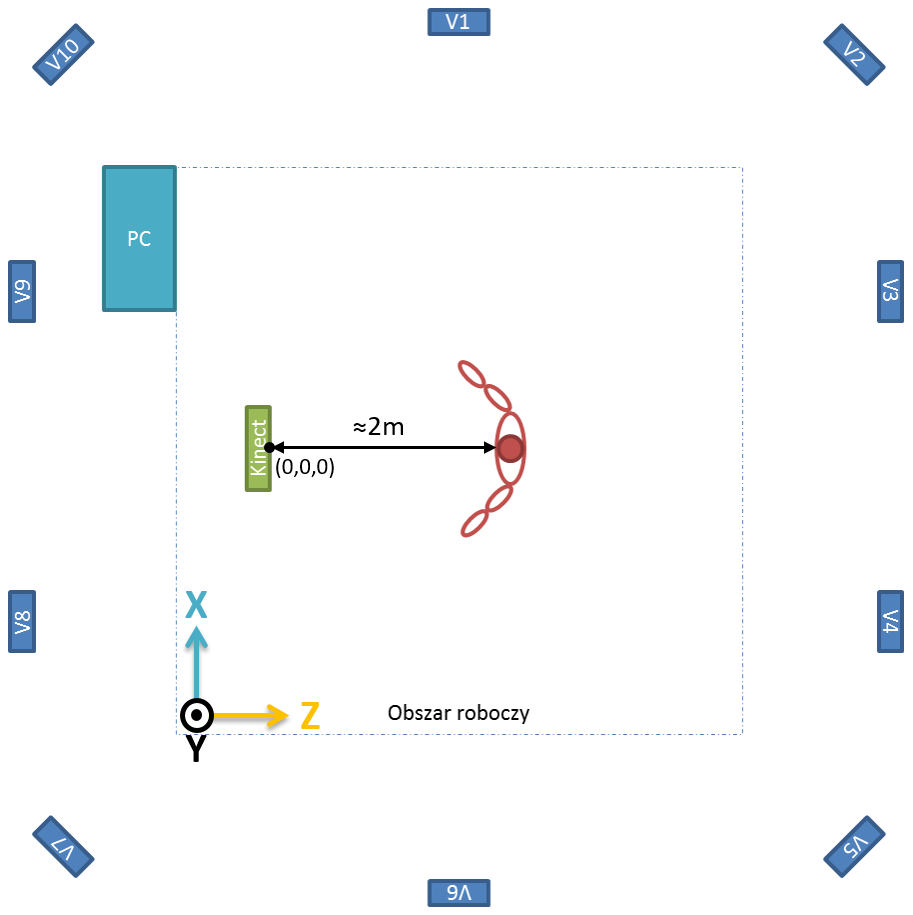
\includegraphics[width=0.7\textwidth]{images/scene.png}
	\caption{Schemat rozmieszczenia elementów sceny w~laboratorium  (źródło: opracowanie własne)}
	\label{fig:experiments:scene}
\end{figure}
		  
		 
Eksperymenty badawcze, opisane w~niniejszej pracy, zostały przeprowadzone na przykładzie ruchu ręki, a~oszacowaniu położenia w~przestrzeni podlegał staw łokciowy oraz nadgarstkowy prawej ręki. Nie ogranicza to jednak możliwości zastosowania opracowanej w~pracy metody do śledzenia pozostałych kończyn. Markery niezbędne do prawidłowego działania systemu śledzenia ruchu firmy Vicon zostały umieszczone według schematu zamieszczonego na rysunku \ref{fig:experiments:viconArm}.
		
\begin{figure}[!htb]
	\centering
	\includegraphics[width=0.75\textwidth]{images/Fig11.png}
	\caption{Schemat romieszczenia markerów na ręce zgodny z~zaleceniami systemu Vicon  (źródło: opracowanie własne)}
	\label{fig:experiments:viconArm}
\end{figure}
				
Sposób umieszczenia markerów został zaczerpnięty ze schematu ich rozmieszczenia zawartego w~instrukcji do systemu Vicon, jednak poszerzony został o~dodatkowe markery tak, aby nadgarstek i~łokieć śledzony był za pomocą czterech znaczników, a~ramię za pomocą trzech. Aby móc skutecznie porównać ze sobą położenie stawów, wyznaczonych na podstawie pomiarów z~kontrolera Kinect i~z czujników inercyjnych, z~tymi wyznaczonymi przez system śledzenia ruchu Vicon, współrzędne śledzonych markerów, reprezentujące wybrany staw, muszą być uśrednione, tak żeby na ich podstawie obliczyć współrzędne stawów analizowanej kończyny. Do dokładnego wyznaczenia pojedynczego punktu reprezentującego staw, pomocne jest oszacowanie położenia trzech markerów. Dzięki zastosowaniu uzupełniających markerów do układu rekomendowanego przez firmę Vicon, udało się znacznie ograniczyć liczbę pomiarów, na których były widoczne mniej niż trzy markery, przez co precyzja śledzenia ruchu kończyn była większa. System śledzenia ruchu Vicon, w~wykorzystanej konfiguracji, dostarczał pomiary co 10 ms -- działał z~częstotliwością 100 Hz.  
				
Oprócz markerów niezbędnych dla poprawnego działania systemu Vicon na przedramieniu i~ramieniu, w~połowie ich długości, zostały umieszczone czujniki inercyjne. Czujniki te, aby możliwie wiernie rejestrować ruchy kończyn zostały przymocowane do skóry za pomocą taśmy klejącej oraz dodatkowo dociśnięte elastycznymi opaskami. Dzięki temu były one w~stanie wykonywać obroty wraz z~kończynami minimalizując względne przesunięcia. Zostały one umieszczone na wierzchniej stronie ręki, tam gdzie jest relatywnie cienka warstwa mięśni i~ścięgien tak jak na rysunku \ref{fig:experiments:handMarker}. Dzięki temu czujniki w~większym stopniu reagowały na obroty kości i~były mniej wrażliwe na pracę otaczających je tkanek (wpływ ruchu między innymi skóry, ścięgień i~mięśni na badanie ruchu kości można znaleźć w~\cite{Sati2016,Reinschmidt2016}).
				
\begin{figure}[!htb]
	\centering
	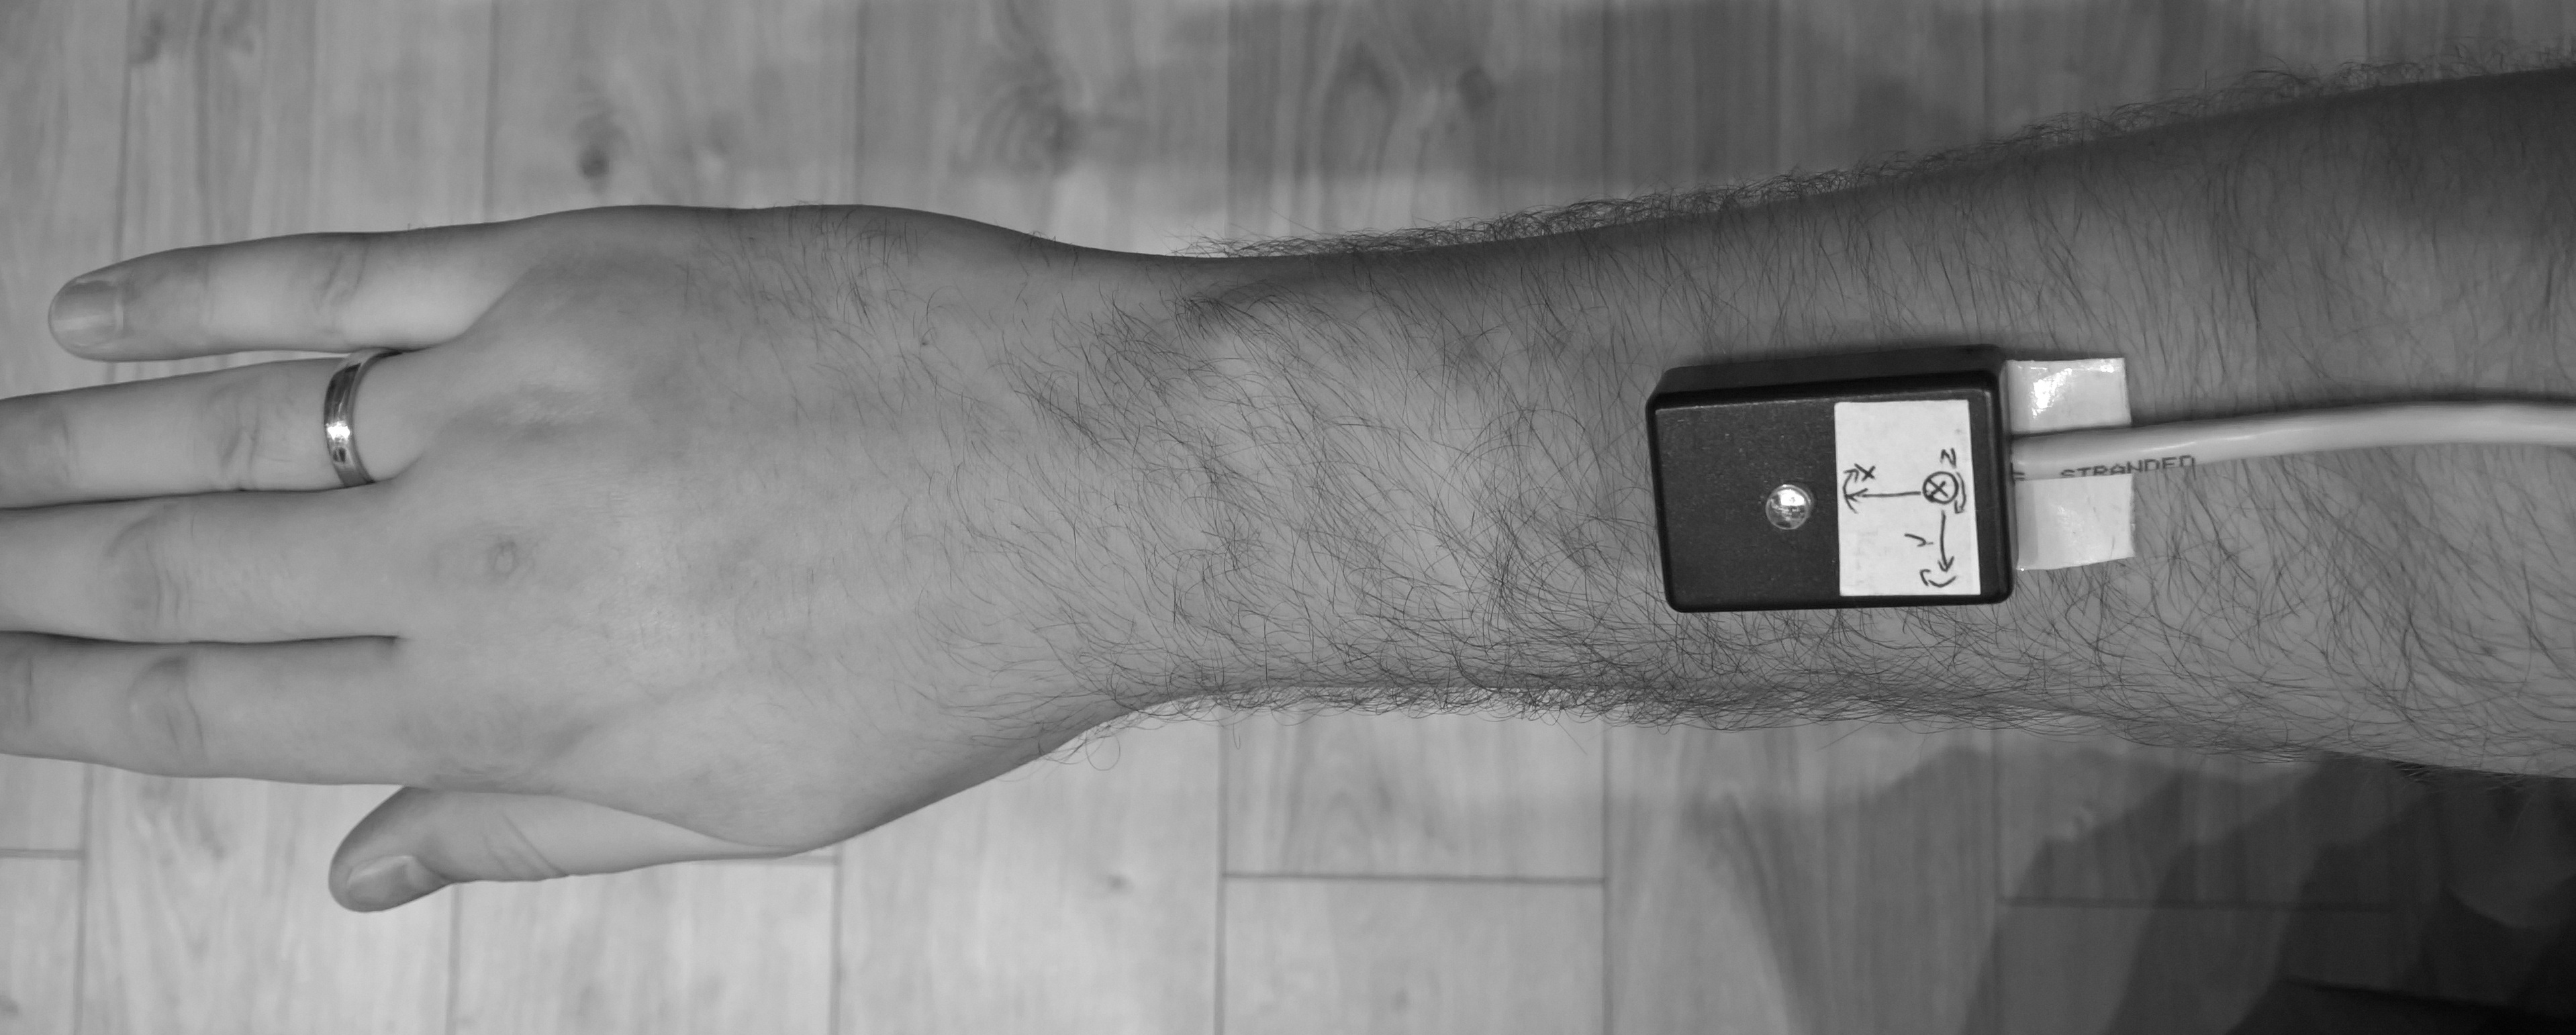
\includegraphics[width=0.9\textwidth]{images/WP_20170423_00_49_25_Raw.jpg}
	\caption{Moduł inercyjny umieszczony na przedramieniu autora(źródło: badania własne)}
	\label{fig:experiments:handMarker}
\end{figure}
				
\section{Badanie ruchu}
				
Każdy z~ruchów ręki był zrealizowany przez trzech użytkowników i~wykonany w~dwóch seriach po pięć powtórzeń. Każda seria stanowiła osobną sesję śledzenia co oznacza, że każdy ruch został zarejestrowany w~sześciu sesjach (3 osoby po 2 sesje śledzenia na każde ćwiczenie). Podzielenie całego ćwiczenia na serie z~mniejszą liczbą powtórzeń związane było z~efektem zmęczenia aktorów, jakie było widoczne wraz z~kolejnymi powtórzeniami. Ćwiczenia jakie należało wykonać zostały dobrane w~taki sposób, aby sprawdzić opisaną metodę zarówno w~sytuacjach, w~których kontroler Kinect i~czujniki inercyjne działają w~uprzywilejowanym dla nich zakresie pracy jak i~w~takich, w~których jedno z~urządzeń posiada istotne ograniczenia w~działaniu. Wszystkie sekwencje rozpoczynały się od pozycji wyjściowej z~rękoma rozłożonymi na boki w~tak zwanej pozycji T (\emph{ang. T--pose}). Następnie, wykonywano zgięcie rąk w~łokciu ku górze (w płaszczyźnie XY) i~ich wyprostowanie w~celu zsynchronizowania pomiarów Kinecta i~czujników inercyjnych w~czasie. Po sekwencji synchronizującej następowały właściwe ćwiczenia, w~których każde powtórzenie zaczynało i~kończyło się pozycją T (\emph{ang. T--pose}). Wykonywane ćwiczenia prezentuje rysunek \ref{fig:experiments:poses}.
			
\begin{figure}[!htb]
	\centering
	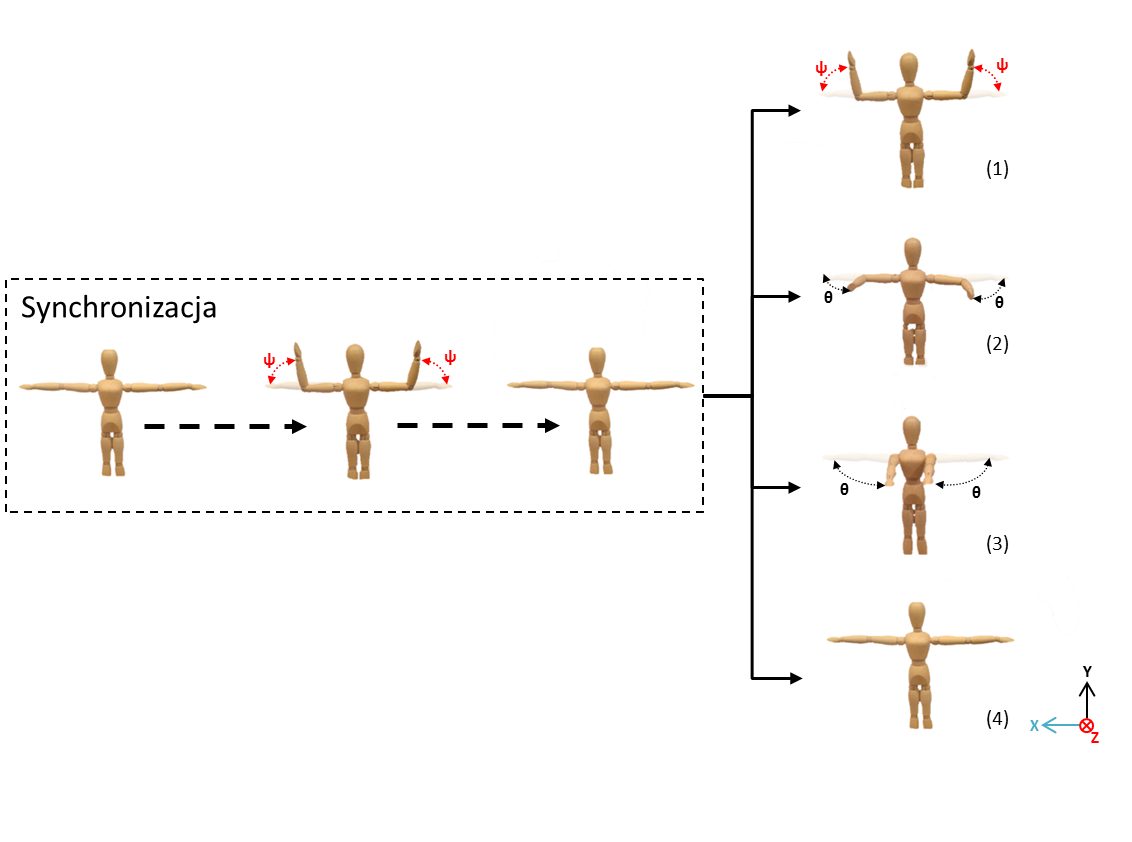
\includegraphics[width=0.9\textwidth]{images/poses.png}
	\caption{Ćwiczenia wykonywane w~ramach eksperymentu  (źródło: badania własne)}
	\label{fig:experiments:poses}
\end{figure}
\newpage				
Lista wykonywanych ćwiczeń obejmuje kolejno:

\begin{enumerate}
	\item Zgięcie ręki w~łokciu do góry (zgięcie w~płaszczyźnie XY układu współrzędnych Kinecta); \\
	\item Zgięcie ręki w~łokciu do przodu (zgięcie w~płaszczyźnie XZ układu współrzędnych Kinecta); \\
	\item Wyciągnięcie wyprostowanych ramion do przodu (ruch w~płaszczyźnie XZ układu współrzędnych Kinecta); \\
	\item Utrzymanie wyprostowanych ramion (pozycja T) w~bezruchu przez czas około 60s; \\
\end{enumerate}
						
Ćwiczenie 1 wykonywane było w~płaszczyźnie, w~której czujniki inercyjne są w~stanie dokonywać dokładnych i~stabilnych w~czasie pomiarów, natomiast dla Kinecta nie następuje okluzja stawów. Ćwiczenia 2 i~3 wymagają wykonania ruchu w~płaszczyźnie, w~której pomiary czujników inercyjnych są błędne i~nie mogą być traktowane jako wiarygodne. Dodatkowo, w~trakcie wykonywania ćwiczenia, kontroler Kinect traci możliwość obserwacji stawów ręki z~powodu ich przesłaniania się. Ostatnie ćwiczenie z~kolei sprawdza stabilność pomiaru w~sytuacji kiedy nie jest wykonywany żaden ruch. Pomiar taki obarczony jest dryfem występującym w~danych uzyskanych za pomocą akcelerometru i~żyroskopu.
						
Wszystkie pomiary zostały porównane z~pomiarami referencyjnymi zarejestrowanymi w~systemie Vicon w~celu określenia dokładności wyznaczania pozycji stawów i~kąta zgięcia w~łokciu. Układy współrzędnych systemu śledzenia Vicon i~systemu opartego na autorskiej metodzie śledzenia ruchu zostały ujednolicone tak aby można było łatwo określić precyzję szacowania położenia stawów. W~trakcie kalibracji systemu Vicon, początek jego układu współrzędnych (punkt $(0,0,0)$) został określony na podłodze, dokładnie pod kontrolerem Kinect, który został także oznaczony markerami w~celu ustalenia jego położenia. Dzięki temu możliwe było uwspólnienie układów współrzędnych Kinecta i~systemu Vicon, a~w~związku z~tym także porównanie ze sobą oszacowań uzyskanych za pomocą obu systemów.

Błąd estymacji pozycji stawów, w~pojedynczej sesji wykonywanego ruchu, został zdefiniowany jako pierwiastek kwadratowy z~błędu średniokwadratowego (RMSE -- \emph{ang. root mean square error}) odległości euklidesowej ($d_e()$) pomiędzy referencyjną pozycją danego stawu ($j$) zmierzoną w~systemie Vicon $P^V_j$, a~pozycją oszacowaną ($P^F_j$) i~jest wyrażony wzorem \ref{eq:experiments:RMSE}

\begin{equation}
	\centering
	RMSE^F_j = \sqrt{\frac{1}{n}\sum_{i=1}^{n}{d_e(P^V_{j,i}, P^F_{j,i})^2}}
	\label{eq:experiments:RMSE}
\end{equation}

Następnie została obliczona średnia arytmetyczna z~wyznaczonych błędów średniokwadratowych każdej z~sesji śledzenia według wzoru \ref{eq:experiments:average}

\begin{equation}
	\overline{RMSE^F_j} = \frac{\sum_{s=1}^{6}{RMSE^F_{j,s}}}{6}
	\label{eq:experiments:average}
\end{equation}

w~celu wyznaczenia dokładności szacowania pozycji stawów w~każdym z~wykonanych ćwiczeń. Podobną metodologię określania błędu oszacowania badanej metody zastosowali w~swoich pracach między innymi Kassim i~in. \cite{Kassim2008} oraz Tadano i~in. \cite{Tadano2013}. W~analogiczny sposób do wzoru \ref{eq:experiments:RMSE} został oszacowany błąd wyznaczania kąta zgięcia stawu łokciowego $\beta$.
						
Błędy szacowania pozycji stawów oraz kąta zgięcia stawu łokciowego zostały wyznaczone dla opisywanej w~niniejszej dysertacji metody łączenia danych, opartej na obrotach kości ($P^{F,O}_j$,$\beta^{F,O}$) oraz dla analogicznych oszacowań uzyskanych za pomocą metody o~najniższym opisanym w~literaturze błędzie szacowania położenia stawów -- metodzie Kalkbrenera i~in. \cite{Kalkbrenner2014}. Metoda Kalkbrenera wykorzystuje  dane o~pozycjach poszczególnych stawów, zarejstrowanych niezaleznie przez kontroler Kinect i~czyjniki inercyjne,
które są łączone celem zmniejszenia niedokładności ($P^{F,P}_j$,$\beta^{F,P}$).
						
Każda z~sesji śledzenia konkretnego ruchu składała się z~5 nieprzerywanych powtórzeń tego samego ruchu. Dla każdej z~takich sesji zostały wyliczone wartości błędu średniokwadratowego każdego z~wyżej wymienionych oszacowań (pozycje stawów łokciowego ($P^F_E, j = E$  \emph{ang. Elbow}) i~nadgarstkowego ($P^F_W, j = W$ \emph{ang. Wrist}) oraz kąt zgięcia łokcia $\beta^F$). Całkowity błąd szacowania metody został określony jako średnia arytmetyczna błedów śrdniokwadratowych ($\overline{RMSE}$) ze wszystkich sześciu sesji śledzenia ruchu (indeks sesji śledzenia -- $s$) dla danego stawu (łokcia $E$ lub nadgarstka $W$) lub kąta $\beta$ (wz. \ref{eq:experiments:average}).

Wyniki zostały zebrane w~tabelach \ref{tab:experiments:first:avg}, \ref{tab:experiments:sec:avg}, \ref{tab:experiments:thr:avg} i~\ref{tab:experiments:four:avg}. Porównanie pomiędzy wynikami uzyskanymi za pomocą metody Kalkbrennera i~metody łączenia danych opartej na obrotach kości zostało wyznaczone jako stosunek procentowy ($r$) różnicy pomiędzy uśrednionym błędem średniokwadratowym dla metody Kalkbrennera ($\overline{RMSE^P_j}$) a~uśrednonym błędem średniokwadratowym dla metody opracowanej przez autora niniejszej dysertacji ($\overline{RMSE^O_j}$) do $\overline{RMSE^P_j}$, gdzie $j$ oznacza analizowany staw szkieletu ($j=E, W$) lub kąt $\beta$ (wz. \ref{eq:experiments:comparison}). \\
						
\begin{equation}
	r = \frac{\overline{RMSE^P_j} - \overline{RMSE^O_j}}{\overline{RMSE^P_j}} * 100\%
	\label{eq:experiments:comparison}
\end{equation}
						
Dodatnia wartość $r$ oznacza, że uśredniony błąd średniokwadratowy wyników uzyskanych za pomocą metody opracowanej przez autora jest mniejszy niż uśredniony błąd średniokwadratowy wyników uzyskanych metodą Kalkbrennera, co oznacza, że nastąpiła poprawa oszacowań. W~przypadku wartości ujemnej mamy do czynienia z~pogorszeniem uzyskiwanych wyników. W~obu przypadkach wartość $r$ określa o~ile procent zmieniły się wyniki. Porównanie uśrednionych błędów średniokwadratowych dla oszacowań:
\begin{itemize}
	\item położenia stawu łokciowego,
	\item położenia stawu nadgarstkowego,
	\item kąta zgięcia stawu łokciowego ($\beta$),
\end{itemize}
wykonanych za pomocą obu metod, zostało zaprezentowane na wykresach znajdujących się w~dalszej części ninejszego rozdziału.
						
\section*{Ćwiczenie 1 -- Zgięcie ramienia w~łokciu do góry}
Pierwsze ćwiczenie, jakie zostało wykonane z~użyciem omawianej metody, to zgięcie ręki w~łokciu do~góry (płaszczyzna XY układu odniesienia). Jest to ruch łatwy do śledzenia dla obu urządzeń pomiarowych ze względu na brak występowania okluzji stawów w~płaszczyźnie ruchu prostopadłej do kierunku obserwacji Kinecta oraz ze względu na to, że nie odbywa się on wokół wektora grawitacji. Wyniki uzyskane w~tym ćwiczeniu prezentuje tabela \ref{tab:experiments:first:avg}.
						
\begin{table}[h]
	\caption[Średni błąd szacowania $\overline{RMSE}$ dla ćwiczenia nr 1]{Średni błąd szacowania $\overline{RMSE}$ (wz. \ref{eq:experiments:comparison})  dla ćwiczenia nr 1 (źródło: badania własne)}
	\label{tab:experiments:first:avg}
	\noindent
	\tiny
	\centering
	\begin{tabular}{|c|c|N{1}{2}|N{1}{2}|N{1}{2}|N{1}{2}|N{1}{2}|N{1}{2}|}		
		\hline 
		\multicolumn{2}{|c|}{}	& \multicolumn{3}{c|}{{Metoda autorska}} & \multicolumn{3}{c|}{{Metoda Kalkbrennera}}  \\ 
		\hline 
		{Użytkownik} & {Sesja}      & {$RMSE^O_E$} & {$RMSE^O_W$} & {$RMSE^O_\beta$} & {$RMSE^P_E$} & {$RMSE^P_W$} & {$RMSE^P_\beta$} \\
		              & {śledzenia} & {$[cm]$}     & {$[cm]$}     & {$[\degree]$}    & {$[cm]$}     & {$[cm]$}     & {$[\degree]$}    \\	
		\hline		
		1             & 1            & 2.2498       & 2.7458       & 3.2398           & 2.6475       & 3.0934       & 3.4396           \\
		1             & 2            & 2.2600       & 2.7635       & 3.3315           & 2.6598       & 3.1049       & 3.7705           \\
		2             & 3            & 2.2308       & 2.7401       & 3.1499           & 2.5496       & 3.0193       & 3.4211           \\
		2             & 4            & 2.2602       & 2.7603       & 3.1825           & 2.5593       & 3.0703       & 3.4827           \\
		3             & 5            & 2.0592       & 2.7814       & 3.3570           & 2.4909       & 2.9371       & 3.5097           \\
		3             & 6            & 2.2603       & 2.7718       & 3.5161           & 2.5602       & 2.9851       & 3.6250           \\
		\hline
		\multicolumn{2}{|c|}{{Średnia $\overline{RMSE}$}} & 2.2200       & 2.7605       & 3.2961           & 2.5779       & 3.0350       & 3.5414           \\
		\multicolumn{2}{|c|}{{Odchylenie}}                 & 0.0727       & 0.0141       & 0.1230           & 0.0585       & 0.0603       & 0.1216           \\
		\hline
	\end{tabular} 																					
\end{table} 								
Ćwiczenie polegające na wielokrotnym zgięciu ręki w~łokciu do góry, zgodnie z~przewidywaniami, dla obu urządzeń pomiarowych nie było trudne. Przez cały czas trwania ćwiczenia stawy były poprawnie identyfikowane i~w~pełni śledzone przez kontroler Kinect. Także czujniki inercyjne były w~stanie zarejestrować w~pełni  wykonywany ruch. Obie porównywane ze sobą metody uzyskiwały podobne wyniki, a~zakres szacowanego przez nie ruchu był zbliżony do tego wykonywanego w~rzeczywistości. Widoczne było natomiast zróżnicowanie w~dopasowaniu szkieletu do ciała ze względu na przyjęty model długości kości. W~metodzie Kalkbrennera miała miejsce częsta zmiana tego oszacowania, co wpływało na to, że śledzony staw potrafił zmienić swoje położenie podczas gdy postać pozostawała w~bezruchu, a~także potrafił znaleźć się poza konturem postaci. W~przypadku metody autora niniejszej rozprawy, zauważalne były częste, jednak niewielkie, fluktuacje wartości oszacowanych pozycji stawów. Były one jednak na tyle niewielkie, że nie wpływały w~istotny sposób na wartość błędu średniokwadratowego uzyskanego szacowania, w~przeciwieństwie do wpływu na ten błąd zmiennej długości segmentów reprezentujących kości wykorzystywanych w~metodzie Kalkbrennera. Wydaje się również, że to właśnie brak stałego modelu długości kości w~metodzie Kalkbrennera ma największy wpływ na różnicę uzyskiwanych wyników w~ćwiczeniu 1. \\
						
W omawianym ćwiczeniu ruch wykonywany był głównie przez przedramię, czyli istotne i~zamierzone zmiany położenia były widoczne na stawie nadgarstkowym. Wykresy \ref{fig:experiments:first:wristX}, \ref{fig:experiments:first:wristY}, \ref{fig:experiments:first:wristZ} pokazują położenie stawu nadgarstkowego w~każdej z~trzech osi w~trakcie wykonywania ruchu. Widać na nich wyraźną różnicę w~stabilności pomiarów objawiającą się ciągłymi drganiami widocznymi na wykresie łączenia danych za pomocą metody Kalkbrennera.
					
\begin{figure}[!htb]
	\centering
	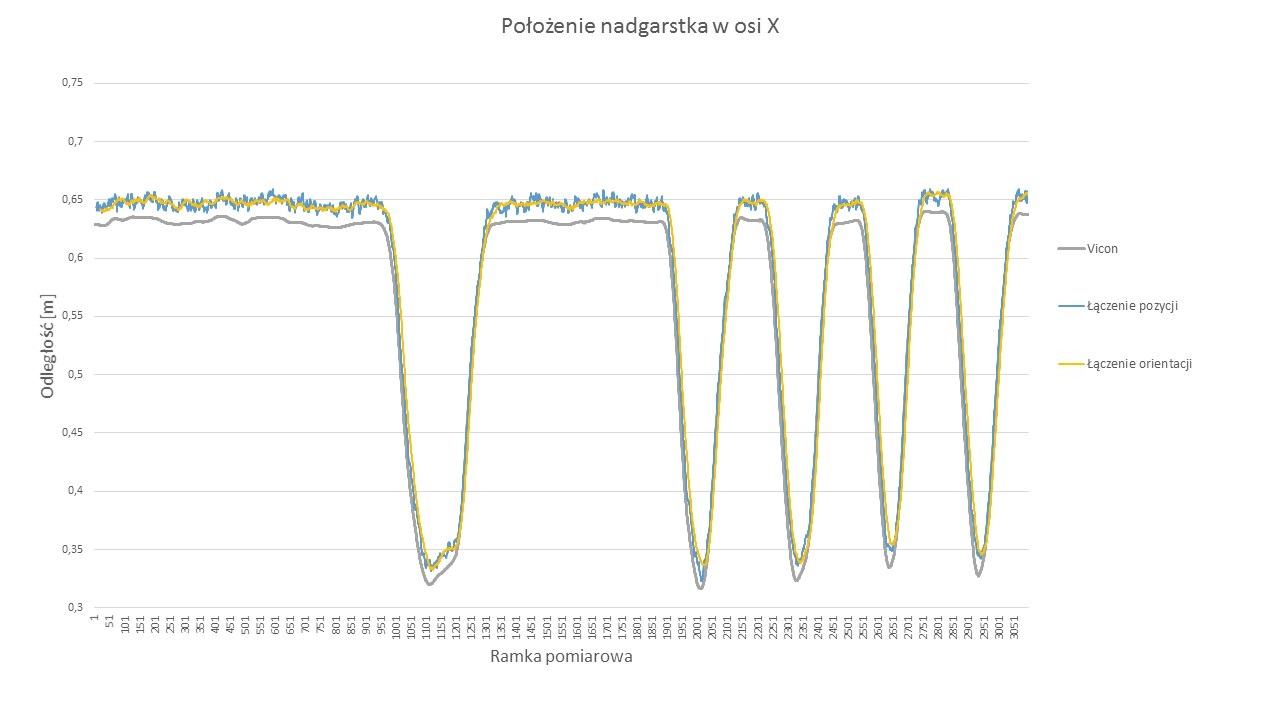
\includegraphics[width=0.9\textwidth]{images/100/Slide4.png}
	\caption{Wykres przedstawiający położenie stawu nadgarstkowego w~osi X w~ćwiczeniu 1 (źródło: badania własne)}
	\label{fig:experiments:first:wristX}
\end{figure}
\begin{figure}[!htb]
	\centering
	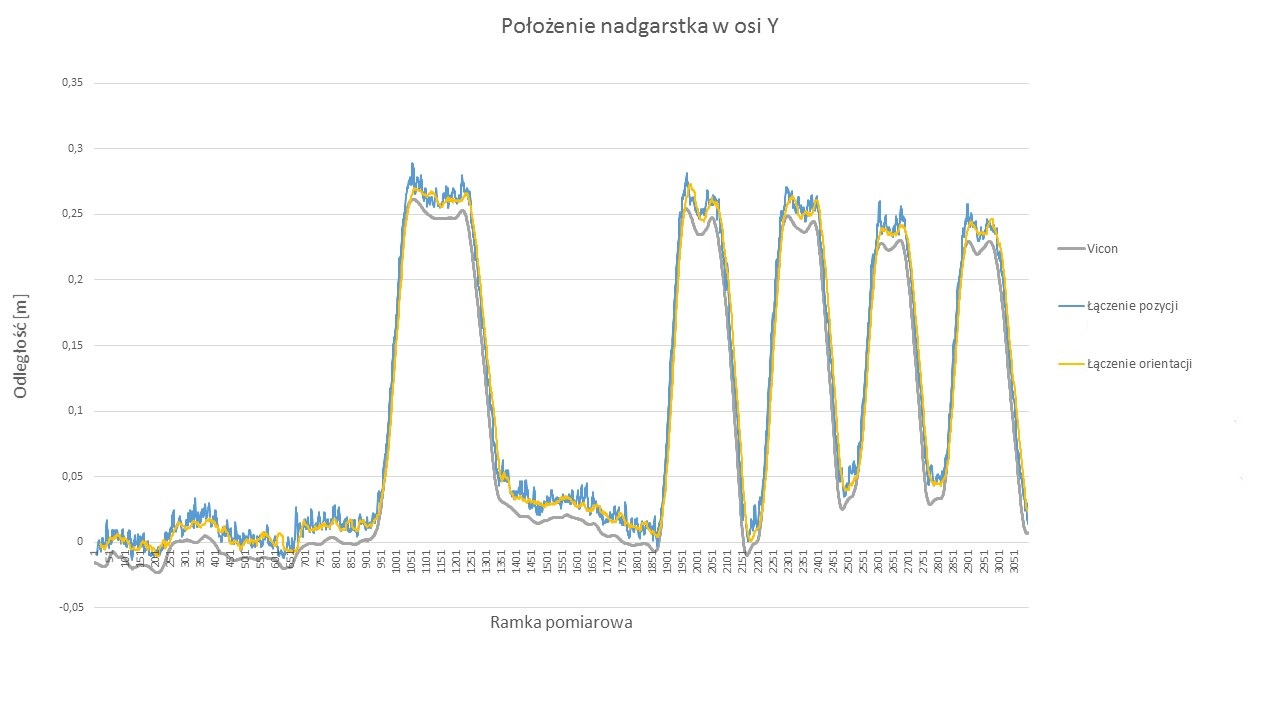
\includegraphics[width=0.9\textwidth]{images/100/Slide5.png}
	\caption{Wykres przedstawiający położenie stawu nadgarstkowego w~osi Y w~ćwiczeniu 1 (źródło: badania własne)}
	\label{fig:experiments:first:wristY}
\end{figure}
\begin{figure}[!htb]
	\centering
	\includegraphics[width=0.9\textwidth]{images/100/Slide6.png}
	\caption{Wykres przedstawiający położenie stawu nadgarstkowego w~osi Z~w~ćwiczeniu 1 (źródło: badania własne)}
	\label{fig:experiments:first:wristZ}
\end{figure}
			
Wykres na rysunku \ref{fig:experiments:first:angle} przedstawia oszacowanie kąta zgięcia ręki w~łokciu ($\beta$). Widać na nim, wyraźną różnicę w~dokładności i~stabilności szacowania wartości w~trakcie wykonywania ruchu oraz w~położeniach skrajnych (wyprostowana ręka lub zgięta). W~położeniu skrajnym widoczne są fluktuacje oszacowań zarówno w~przypadku metody Kalkbrennera jak i~metody autorskiej. Jednakże fluktuacje obecne w~oszacowaniach metody, łączącej ze sobą obroty są, widocznie mniejsze niż te występujące w~metodzie opartej o~łączenie pozycji stawów.
			
\begin{figure}[!htb]
	\centering
	\includegraphics[width=0.9\textwidth]{images/100/angle.png}
	\caption{Wykres przedstawiający oszacowanie wartości kąta zgięcia ręki w~łokciu ($\beta$) w~ćwiczeniu 1 (źródło: badania własne)}
	\label{fig:experiments:first:angle}
\end{figure}
												
Rysunki \ref{fig:experiments:first:raw} oraz \ref{fig:experiments:first:fused} wizualizują ruch ręki podczas tego ćwiczenia. W~przypadku obu metod łączenia danych widać poprawę pozycjonowania stawów względem danych otrzymanych bezpośrednio z~urządzeń pomiarowych. 
					
\begin{figure}[!htb]
	\captionsetup{singlelinecheck=off}
	\centering
	\begin{subfigure}[b]{0.48\textwidth}
		\centering
		\includegraphics[width=0.9\textwidth]{images/100/raw.png}	
		\caption{Wizualizacja ruchu bezpośrednio z~urządzeń pomiarowych}
		\label{fig:experiments:first:raw}
	\end{subfigure}
	\hfill																														
	\begin{subfigure}[b]{0.48\textwidth}
		\centering
		\includegraphics[width=0.9\textwidth]{images/100/Fused.png}		
		\caption{Wizualizacja ruchu po złączeniu danych z~urządzeń pomiarowych}
		\label{fig:experiments:first:fused}	
	\end{subfigure}																														
	\caption[Wizualizacja ruchu ręki w~ćwiczeniu 1]{Wizualizacja ruchu ręki w~ćwiczeniu 1.  Kolory: czarny -- Vicon, niebieski -- czujniki inercyjne, zielony -- Kinect, szary -- metoda Kalkbrennera, pomarańczowy -- metoda autorska (źródło: badania własne)}	
	\label{fig:experiments:first}
\end{figure}
														
\section*{Ćwiczenia 2 i~3 -- Zgięcie ramienia w~łokciu do przodu oraz wyciągnięcie wyprostowanych ramion do przodu}
Ćwiczenia 2 i~3 przedstawiają ruchy o~zwiększonym stopniu trudności śledzenia dla obu urządzeń pomiarowych. W~tym przypadku następuje stopniowe przysłanianie jednego ze stawów co oznacza utratę możliwości dokładnego śledzenia ruchu przez kontroler Kinect. Dodatkowo ruch odbywał się w~płaszczyźnie trudnej z~punktu widzenia czujników inercyjnych, ponieważ obrót dokonywany był wokół osi równoległej do wektora grawitacji. Tabela \ref{tab:experiments:sec:avg} przedstawia średnie dokładności wykonywanego ruchu samego przedramienia, natomiast tabela \ref{tab:experiments:thr:avg} przedstawia wyniki dla ruchu całej wyprostowanej ręki.
														
\begin{table}[h]
	\caption[Średni błąd szacowania $\overline{RMSE}$ dla ćwiczenia nr 2]{Średni błąd szacowania $\overline{RMSE}$ (wz. \ref{eq:experiments:comparison}) dla ćwiczenia nr 2 (źródło: badania własne)}
	\label{tab:experiments:sec:avg}
	\noindent
	\tiny
	\centering
	\begin{tabular}{|c|c|N{1}{2}|N{1}{2}|N{2}{2}|N{1}{2}|N{1}{2}|N{2}{2}|}		
		\hline 
		\multicolumn{2}{|c|}{}	& \multicolumn{3}{c|}{{Metoda autorska}} & \multicolumn{3}{c|}{{Metoda Kalkbrennera}}  \\ 
		\hline 
		{Użytkownik} & {Sesja}      & {$RMSE^O_E$} & {$RMSE^O_W$} & {$RMSE^O_\beta$} & {$RMSE^P_E$} & {$RMSE^P_W$} & {$RMSE^P_\beta$} \\
		              & {śledzenia} & {$[cm]$}     & {$[cm]$}     & {$[\degree]$}    & {$[cm]$}     & {$[cm]$}     & {$[\degree]$}    \\	
		\hline			
		1             & 1            & 2.6659       & 3.0214       & 14.4574          & 3.0815       & 3.4849       & 15.0134          \\
		1             & 2            & 2.4977       & 2.8483       & 12.7191          & 3.0676       & 3.5101       & 13.0746          \\
		2             & 3            & 2.3591       & 2.7377       & 12.7836          & 2.8575       & 3.2409       & 14.4970          \\
		2             & 4            & 2.4143       & 2.9260       & 13.3775          & 3.1409       & 3.5275       & 15.2791          \\
		3             & 5            & 2.4451       & 2.8774       & 13.4106          & 3.1591       & 3.4737       & 14.6086          \\
		3             & 6            & 2.5134       & 2.7932       & 13,3402          & 2.9532       & 3,5042       & 14.5012          \\		
		\hline
		\multicolumn{2}{|c|}{{Średnia $\overline{RMSE}$}} & 2.4826       & 2.8673       & 13.3480          & 3.0613       & 3.4569       & 14.4957          \\
		\multicolumn{2}{|c|}{{Odchylenie}}                            & 0.1048       & 0.0931       & 0.6244           & 0.1075       & 0.1049       & 0.7634           \\
		\hline
	\end{tabular} 																																					
\end{table} 
														
\begin{table}[h]
	\caption[Średni błąd szacowania $\overline{RMSE}$ dla ćwiczenia nr 3]{Średni błąd szacowania $\overline{RMSE}$ (wz. \ref{eq:experiments:comparison}) dla ćwiczenia nr 3 (źródło: badania własne)}
	\label{tab:experiments:thr:avg}
	\noindent
	\tiny
	\centering
	\begin{tabular}{|c|c|N{1}{2}|N{1}{2}|N{2}{2}|N{1}{2}|N{1}{2}|N{2}{2}|}		
		\hline 
		\multicolumn{2}{|c|}{}	& \multicolumn{3}{c|}{{Metoda autorska}} & \multicolumn{3}{c|}{{Metoda Kalkbrennera}}  \\ 
		\hline 
		{Użytkownik} & {Sesja}      & {$RMSE^O_E$} & {$RMSE^O_W$} & {$RMSE^O_\beta$} & {$RMSE^P_E$} & {$RMSE^P_W$} & {$RMSE^P_\beta$} \\
		              & {śledzenia} & {$[cm]$}     & {$[cm]$}     & {$[\degree]$}    & {$[cm]$}     & {$[cm]$}     & {$[\degree]$}    \\	
		\hline		
		1             & 1            & 2.5959       & 2.9683       & 13.3184          & 3.1288       & 3.5589       & 15.7465          \\
		1             & 2            & 2.2391       & 2.5266       & 12.3694          & 2.9860       & 3.3287       & 13.1241          \\
		2             & 3            & 2.7619       & 3.1413       & 13.1813          & 2.7030       & 3.1432       & 12.5385          \\
		2             & 4            & 2.7347       & 3.0278       & 14.7809          & 3.1662       & 3.5129       & 16.4055          \\
		3             & 5            & 2.2166       & 2.5777       & 16.7666          & 2.7412       & 3.0710       & 15.7460          \\
		3             & 6            & 2.1975       & 2.6912       & 13.4102          & 2.7532       & 2.9042       & 14.6612          \\
		\hline																		
		\multicolumn{2}{|c|}{{Średnia $\overline{RMSE}$}} & 2.4576       & 2.8222       & 13.9711          & 2.9131       & 3.2531       & 14.7036          \\
		\multicolumn{2}{|c|}{{Odchylenie}}                            & 0.2456       & 0.2344       & 1.4376           & 0.1893       & 0.2358       & 1.4291           \\
		\hline
	\end{tabular} 																																					
\end{table} 
														
W obu ćwiczeniach, w~trakcie wykonywania ruchu, następował moment, w~którym jeden lub dwa stawy stawały się niewidoczne dla kontrolera Kinect, a~co za tym idzie, obie metody musiały bazować tylko na jednym źródle danych. Metoda opracowana przez autora niniejszej pracy nie wykorzystywała  w~trakcie łączenia danych pomiarów uzyskanych z~niepewnego źródła i~stopniowo wstrzymywała aktualizację estymowanego położenia stawu. Natomiast metoda Kalkbrennera wykorzystywała w~dalszym ciągu dane z~kontrolera Kinect zmieniając jedynie ich stopień istotności (rys. \ref{fig:experiments:sec:follow}). 
														
Ze względu na to, że kontroler Kinect, pomimo utraty możliwości śledzenia wybranego stawu, wciąż estymuje jego położenie, zasadne jest sprawdzanie czy fuzja pomiarów dostarczonych przez kontroler Kinect z~pomiarami urządzeń inercyjnych nie sprawi, że ostateczna estymacja położenia stawu stanie się zbyt niedokładna. Metoda Kalkbrennera co prawda dokonuje takiego sprawdzenia w~trakcie stosowania filtru Kalmana, jednak widoczne było podążanie szacunkowych wartości położenia stawu za skokami danych z~Kinecta. Oznacza to, że wpływ pomiarów kontrolera Kinect na ostateczną estymację jest znaczący i~zastosowana w~metodzie Kalkbrennera zmiana stopnia ich istotności, w~procesie łączenia danych, jest niewystarczająca na ograniczenie negatywnego wpływu niedokładności kontrolera Kinect.
				
\begin{figure}[!htb]
	\centering
	\includegraphics[width=0.9\textwidth]{images/300/Slide3_focus.png}
	\caption{Wykres przedstawiający podążanie wyznaczania pozycji stawu za pomiarami Kinecta w~ćwiczeniu 3 (źródło: badania własne)}
	\label{fig:experiments:sec:follow}
\end{figure}
\begin{figure}[!htb]
	\captionsetup{singlelinecheck=off}
	\centering
	\begin{subfigure}[b]{0.48\textwidth}
		\centering
		\includegraphics[width=0.9\textwidth]{images/200/raw.png}	
		\caption{Wizualizacja ruchu bezpośrednio z~urządzeń pomiarowych}
		\label{fig:experiments:sec:raw}
	\end{subfigure}
	\hfill																																	
	\begin{subfigure}[b]{0.48\textwidth}
		\centering
		\includegraphics[width=0.9\textwidth]{images/200/Fused.png}		
		\caption{Wizualizacja ruchu po złączeniu danych z~urządzeń pomiarowych}
		\label{fig:experiments:sec:fused}
	\end{subfigure}
																																									
	\caption[Wizualizacja ruchu ręki w~ćwiczeniu 2]{Wizualizacja ruchu ręki w~ćwiczeniu 2.  Kolory: czarny -- Vicon, niebieski -- czujniki inercyjne, zielony -- Kinect, szary -- metoda Kalkbrennera, pomarańczowy -- metoda autorska (źródło: badania własne)}	
	\label{fig:experiments:sec}
\end{figure}

\begin{figure}[!htb]
	\captionsetup{singlelinecheck=off}
	\centering
	\begin{subfigure}[b]{0.48\textwidth}
		\centering
		\includegraphics[width=0.9\textwidth]{images/300/raw.png}	
		\caption{Wizualizacja ruchu bezpośrednio z~urządzeń pomiarowych}
		\label{fig:experiments:th:raw}
	\end{subfigure}
	\hfill																																				
	\begin{subfigure}[b]{0.48\textwidth}
		\centering
		\includegraphics[width=0.9\textwidth]{images/300/Fused.png}		
		\caption{Wizualizacja ruchu po złączeniu danych z~urządzeń pomiarowych}
		\label{fig:experiments:th:fused}	
	\end{subfigure}
																																											
	\caption[Wizualizacja ruchu ręki w~ćwiczeniu 3]{Wizualizacja ruchu ręki w~ćwiczeniu 3.  Kolory: czarny -- Vicon, niebieski -- czujniki inercyjne, zielony -- Kinect, szary -- metoda Kalkbrennera, pomarańczowy -- metoda autorska (źródło: badania własne)}	
	\label{fig:experiments:th}
\end{figure}
																				
Rysunki \ref{fig:experiments:sec:raw} i~\ref{fig:experiments:th:raw} przedstawiają wizualizację położenia stawów ręki, których położenie wyestymowano na podstawie pomiarów uzyskanych bezpośrednio z~urządzeń pomiarowych. Widoczne na nich jest niedokładne szacowanie położenia stawu łokciowego przez kontroler Kinect w~momencie jego przysłonięcia, a~z tym związane jest także niedokładne szacowanie położenia nadgarstka, pomimo jego pełnej widoczności. Widoczne jest także błędne szacowanie obrotu zarówno kości przedramienia jak i~ramienia wokół osi grawitacji przez urządzenia inercyjne. Wizualizuje to w~pełni ograniczenia w~działaniu obu urządzeń pomiarowych, które zostały opisane w~rozdziale \ref{chap:characteristics}. W~przypadku wizualizacji pozycjonowania stawów łokciowego i~nadgarstkowego, za pomocą metody Kalkbrennera oraz metody autora niniejszej rozprawy (rys. \ref{fig:experiments:sec:fused} oraz \ref{fig:experiments:th:fused}), w~obu przypadkach widoczne jest zmniejszenie wpływu występowania okluzji stawów jak i~błędów pomiaru obrotu wokół osi grawitacji na ostateczne szacowanie położenia stawów. Widać równocześnie wierniejsze odwzorowanie ruchu w~przypadku metody autora.\\
				
Wykresy z~rysunków \ref{fig:experiments:second:angle} i~\ref{fig:experiments:third:angle} przedstawiają oszacowania wartości kąta $\beta$ w~trakcie wykonywania ćwiczeń 2 i~3. Porównując ze sobą oba te wykresy, można zauważyć znacząco większe fluktuacje uzyskanych wyników szacowania wartości kąta $\beta$ w~ćwiczeniu 3 niż w~ćwiczeniu 2. W~obu tych ćwiczeniach dochodziło do czasowego przysłonięcia stawów ręki, w~ćwiczeniu 2 tylko łokcia, natomiast w~ćwiczeniu 3 zarówno łokcia jak i~barku. Skutkowało to pogorszeniem jakości pomiarów Kinecta co miało bezpośredni wpływ na działanie obu metod łączenia danych. W~obu przypadkach można zauważyć, że fluktuacje wyników uzyskanych za pomocą metody łączącej informację o~obrotach (metody autora pracy) były mniejsze od tych uzyskanych za pomocą metody opartej o~łączenie pozycji stawów.
				
\begin{figure}[!htb]
	\centering
	\includegraphics[width=0.9\textwidth]{images/200/angle.png}
	\caption{Wykres przedstawiający oszacowanie wartości kąta zgięcia ręki w~łokciu ($\beta$) w~ćwiczeniu 2 (źródło: badania własne)}
	\label{fig:experiments:second:angle}
\end{figure}
\begin{figure}[!htb]
	\centering
	\includegraphics[width=0.9\textwidth]{images/300/angle.png}
	\caption{Wykres przedstawiający oszacowanie wartości kąta zgięcia ręki w~łokciu ($\beta$) w~ćwiczeniu 3  (źródło: badania własne)}
	\label{fig:experiments:third:angle}
\end{figure}
																				
\section*{Ćwiczenie 4 -- Utrzymanie wyprostowanych ramion}
Celem ostatniego ćwiczenia było sprawdzenie stabilności pomiarów w~przypadku długiego braku ruchu. W~tym wypadku urządzeniem, którego dane pomiarowe mogą szczególnie ulec pogorszeniu w~trakcie działania jest urządzenie zbudowane z~czujników inercyjnych. Tabela \ref{tab:experiments:four:avg} zawiera zestawienie dokładności pomiarów dla tego eksperymentu.
																				
\begin{table}[!htb]
	\caption[Średni błąd szacowania $\overline{RMSE}$ dla ćwiczenia nr 4]{Średni błąd szacowania $\overline{RMSE}$ (wz. \ref{eq:experiments:comparison}) dla ćwiczenia nr 4 (źródło: badania własne)}
	\label{tab:experiments:four:avg}
	\noindent
	\tiny
	\centering
	\begin{tabular}{|c|c|N{1}{2}|N{1}{2}|N{1}{2}|N{1}{2}|N{1}{2}|N{1}{2}|}		
		\hline 
		\multicolumn{2}{|c|}{}	& \multicolumn{3}{c|}{{Metoda autorska}} & \multicolumn{3}{c|}{{Metoda Kalkbrennera}}  \\ 
		\hline 
		{Użytkownik} & {Sesja}      & {$RMSE^O_E$} & {$RMSE^O_W$} & {$RMSE^O_\beta$} & {$RMSE^P_E$} & {$RMSE^P_W$} & {$RMSE^P_\beta$} \\
		              & {śledzenia} & {$[cm]$}     & {$[cm]$}     & {$[\degree]$}    & {$[cm]$}     & {$[cm]$}     & {$[\degree]$}    \\	
		\hline		
		1             & 1            & 2.1208       & 2.3861       & 4.5450           & 2.3990       & 2.7321       & 4.8643           \\
		1             & 2            & 2.2612       & 2.6185       & 3.8645           & 2.4400       & 2.7574       & 5.1007           \\
		2             & 3            & 2.1646       & 2.4969       & 3.6962           & 2.5821       & 2.8521       & 4.2370           \\
		2             & 4            & 2.3011       & 2.5810       & 4.2258           & 2.5777       & 2.8544       & 4.6130           \\
		3             & 5            & 2.5827       & 2.4711       & 4.3170           & 2.4692       & 2.7876       & 4.8454           \\
		3             & 6            & 2.1827       & 2.4813       & 4.0222           & 2.3609       & 2.7499       & 4.2690           \\
		\hline															
		\multicolumn{2}{|c|}{{Średnia $\overline{RMSE}$}} & 2.2688       & 2.5058       & 4.1118           & 2.4715       & 2.7889       & 4.6549           \\
		\multicolumn{2}{|c|}{{Odchylenie}}                            & 0.1526       & 0.0758       & 0.2842           & 0.0836       & 0.0483       & 0.3173           \\
		\hline
	\end{tabular} 
																																												
\end{table} 
																				
Podobnie jak w~ćwiczeniu 1, tak i~w~ćwiczeniu 4, oba urządzenia były w~stanie śledzić ruchy wykonywane przez śledzonego aktora przez cały czas trwania eksperymentu. Jednak, podobnie jak we wspomnianym ćwiczeniu, zmianie ulegały długości segmentów kości i~miało to przełożenie na działanie metody Kalkbrennera. Wizualizacje łańcuchów kinematycznych przedstawione na rysunku \ref{fig:experiments:four} pokazują, że Kinect, mimo pełnej widoczności całej ręki, miał trudność z~poprawnym określeniem jej pozycji w~osi pionowej. Mimo to obie metody były w~stanie wyznaczyć pozycje stawów z~lepszą dokładnością niż każde z~urządzeń pomiarowych osobno.

\begin{figure}[!htb]
	\captionsetup{singlelinecheck=off}
	\centering
	\begin{subfigure}[b]{0.48\textwidth}
		\centering
		\includegraphics[width=0.9\textwidth]{images/400/raw.png}	
		\caption{Wizualizacja ruchu bezpośrednio z~urządzeń pomiarowych}
		\label{fig:experiments:four:raw}
	\end{subfigure}
	\hfill																																											
	\begin{subfigure}[b]{0.48\textwidth}
		\centering
		\includegraphics[width=0.9\textwidth]{images/400/Fused.png}		
		\caption{Wizualizacja ruchu po złączeniu danych z~urządzeń pomiarowych}
		\label{fig:experiments:four:fused}	
	\end{subfigure}
																																													
	\caption[Wizualizacja ruchu ręki w~ćwiczeniu 4]{Wizualizacja ruchu ręki w~ćwiczeniu 4.  Kolory: czarny -- Vicon, niebieski -- czujniki inercyjne, zielony -- Kinect, szary -- metoda Kalkbrennera, pomarańczowy -- metoda autorska (źródło: badania własne)}	
	\label{fig:experiments:four}
\end{figure}
																						
Wykresy estymacji położenia stawu łokciowego (rys. \ref{fig:experiments:four:elbowZ}) oraz nadgarstkowego (rys. \ref{fig:experiments:four:wristZ}) pozwalają zaobserwować wpływ stabilności pomiarów jednego stawu na drugi. Jest to szczególnie widoczne w~wykresie metody Kalkbrennera, gdzie amplituda drgań pozycji nadgarstka jest widocznie większa niż w~przypadku drgań łokcia. 
					
\begin{figure}[!htb]
	\centering	
		\includegraphics[width=0.9\textwidth]{images/400/3.png}		
		\caption[Wykres położenia stawu łokciowego w~osi Z~w~ćwiczeniu 4]{Wykres położenia stawu łokciowego w~osi Z~w~ćwiczeniu 4 (źródło: badania własne)}
		\label{fig:experiments:four:elbowZ}
\end{figure}
\begin{figure}[!htb]
	\centering
		\includegraphics[width=0.9\textwidth]{images/400/6.png}		
		\caption[Wykres położenia stawu nadgarstkowego w~osi Z~w~ćwiczeniu 4]{Wykres położenia stawu nadgarstkowego w~osi Z~w~ćwiczeniu 4 (źródło: badania własne)}	
		\label{fig:experiments:four:wristZ}
\end{figure}
		
Wykres estymacji kąta $\beta$ w~trakcie ćwiczenia 4, zaprezentowany na rysunku \ref{fig:experiments:fourth:angle}, pozwala zauważyć podobne zachowanie estymowanych wartości kąta do tego zaobserwowanego w~ćwiczeniu 1. W~trakcie wykonywania ruchu (w tym ćwiczeniu zamierzona zmiana kąta w~łokciu następowała tylko podczas początkowej synchronizacji) widać estymację kąta za pomocą obu metod zbliżoną do danych referencyjnych. Różnica jest natomiast dobrze widoczna podczas braku ruchu. Wówczas widoczne są wyraźne fluktuacje w~oszacowaniach wartości kąta, które wpływają na wartość uzyskanego błędu średniowkadratowego.
			
\begin{figure}[!htb]
	\centering
	\includegraphics[width=0.9\textwidth]{images/400/angle.png}
	\caption{Wykres przedstawiający oszacowanie wartości kąta zgięcia ręki w~łokciu ($\beta$) w~ćwiczeniu 4 (źródło: badania własne)}
	\label{fig:experiments:fourth:angle}
\end{figure}
														
\section{Podsumowanie}																								
Ćwiczenia wykonywane w~ramach eksperymentów miały za zadanie zweryfikować dokładność metody autora niniejszej pracy, i~porównać ją z~metodą Kalkbrennera w~sytuacji, gdy pomiary z~czujników przestają być wiarygodne oraz kiedy są one degradowane w~czasie. Dla kontrastu weryfikacja dokładności porównywanych metod, dokonana została także na bazie ćwiczenia, które dla obu urządzeń pomiarowych może być nazywane neutralnym (ćwiczenie 1).
																								
Porównane ze sobą zostały wartości trzech parametrów wybranego układu szkieletowego, wyznaczone przez dwie metody: metodę Kalkbrennera i~metodę łączącą dane opartą o~obroty kości. Porównanymi parametrami kończyny górnej były: położenie stawu łokciowego, położenie stawu nadgarstkowego oraz kąt zgięcia ręki w~łokciu ($\beta$). Błąd oszacowania pozycji stawów w~przestrzeni (wz. \ref{eq:experiments:average}) może być wykorzystany jako wskaźnik na ile dana metoda mogłaby być wykorzystana tam gdzie istotne jest wykrycie czy dochodzi do interakcji pomiędzy estymowanym modelem a~otoczeniem. Jako przykład można podać środowisko wirtualne, w~którym znajdują się obiekty, którymi można manipulować. Każdy taki obiekt ma swoje ściśle określone położenie w~przestrzeni, a~estymacja pozycji stawów jest niezbędna żeby określić czy doszło do interakcji z~takim obiektem czy nie.
																								 
Trzeci parametr układu szkieletowego ręki -- kąt zgięcia ręki w~łokciu ($\beta$) -- jest uniezależniony od przyjętych długości kości i~ewentualnych błędów w~pomiarach tych długości. Określa on wzajemną orientację, pomiędzy kością przedramienia a~ramieniem, w~zakresie stopnia swobody stawu łokciowego. Pozwala też na zweryfikowanie śledzenia zakresu ruchu stawu łokciowego na potrzeby ruchu, co może być przydatne w~procesie rehabilitacji ruchowej. 

\begin{figure}[!htb]
	\centering
	\begin{tikzpicture}
		\begin{axis}[
				ybar,
				bar width=.5cm,
				width=0.9\textwidth,
				height=.5\textwidth,
				legend style={at={(0.5,1)},
					anchor=north,legend columns=-1},
				symbolic x coords={ex 1,ex 2,ex 3,ex 4},
				xticklabels={Ćwiczenie 1,Ćwiczenie 2,Ćwiczenie 3,Ćwiczenie 4},
				xtick=data,
				ymin=0,ymax=5,
				ylabel={$\overline{RMSE} [cm]$},
			]
			\addplot [black,fill=white,error bars/.cd,y dir=both,y explicit] coordinates { 
				(ex 1,2.6) +- (0.0, 0.07)         
				(ex 2,3.1) +- (0.0, 0.11)
				(ex 3,2.9) +- (0.0, 0.18)  
			(ex 4,2.5) +- (0.0, 0.08) };
			\addplot [black,fill=gray80,error bars/.cd,y dir=both,y explicit] coordinates { 
				(ex 1,2.2) +- (0.0, 0.08)         
				(ex 2,2.5) +- (0.0, 0.14)
				(ex 3,2.5) +- (0.0, 0.23)  
			(ex 4,2.3) +- (0.0, 0.16) };
			\legend{Metoda Kalkbrennera, Metoda autorska}
			\node at (axis cs:ex 1,4){\textcolor{black}{r = 13\%}};
			\node at (axis cs:ex 2,4){\textcolor{black}{r = 18\%}};
			\node at (axis cs:ex 3,4){\textcolor{black}{r = 14\%}};
			\node at (axis cs:ex 4,4){\textcolor{black}{r = 7\%}};
		\end{axis}
	\end{tikzpicture}	
	\caption{Średni błąd średniokwadratowy wyznaczania pozycji łokcia (źródło: badania własne)}
	\label{fig:experiments:elbow:summary}
\end{figure}

\begin{figure}[!htb]
	\centering
	\begin{tikzpicture}
		\begin{axis}[
				ybar,
				bar width=.5cm,
				width=0.9\textwidth,
				height=.5\textwidth,
				legend style={at={(0.5,1)},
					anchor=north,legend columns=-1},
				symbolic x coords={ex 1,ex 2,ex 3,ex 4},
				xtick=data,
				ymin=0,ymax=5,
				xticklabels={Ćwiczenie 1,Ćwiczenie 2,Ćwiczenie 3,Ćwiczenie 4},
				ylabel={$\overline{RMSE} [cm]$},
			]
			\addplot [black,fill=white,error bars/.cd,y dir=both,y explicit] coordinates { 
				(ex 1,3.0) +- (0.0, 0.05)
				(ex 2,3.4) +- (0.0, 0.1)
				(ex 3,3.3) +- (0.0, 0.24)
			(ex 4,2.8) +- (0.0, 0.04)};
			\addplot [black,fill=gray80,error bars/.cd,y dir=both,y explicit] coordinates { 
				(ex 1,2.9) +- (0.0, 0.07)
				(ex 2,2.9) +- (0.0, 0.12)
				(ex 3,2.8) +- (0.0, 0.2)
			(ex 4,2.5) +- (0.0, 0.07)};
		
			\legend{Metoda Kalkbrennera, Metoda autorska}
			\node at (axis cs:ex 1,4){\textcolor{black}{r = 8\%}};
			\node at (axis cs:ex 2,4){\textcolor{black}{r = 16\%}};
			\node at (axis cs:ex 3,4){\textcolor{black}{r = 14\%}};
			\node at (axis cs:ex 4,4){\textcolor{black}{r = 9\%}};
		\end{axis}
	\end{tikzpicture}
	\caption{Średni błąd średniokwadratowy wyznaczania pozycji nadgarstka (źródło: badania własne)}
	\label{fig:experiments:wrist:summary}
\end{figure}

Wykresy z~rysunków \ref{fig:experiments:elbow:summary}, \ref{fig:experiments:wrist:summary} oraz \ref{fig:experiments:angle:summary} pokazują podsumowanie porównania uśrednionych wartości błędu uzyskanych oszacowań ($\overline{RMSE}$) za pomocą metody Kalkbrennera oraz metody autora tej pracy.
%([TODO] teraz czuje, że metoda powinna mieć jakiś skrót, np. od angielskiej jej nazwy, którą pewnie trzeba wymyśleć - Oriented-based Hybrid Motion Tracking -> OHMT => najbliżej jest MOTH tylko jak? / Jest jeszcze HOMT -> Hybrid, Oriented-based Motion Tracking tylko ten skrótowiec występuje też w~slangu: http://www.urbandictionary.com/define.php?term=H.O.M.T. ). 
Widać na~nich poprawę w~wyznaczaniu położenia stawu łokciowego do 18\%, nadgarstowego do 16\% oraz zdolności szacowania kąta zgięcia ręki w~łokciu do 11\%. Z~uzyskanych rezultatów eksperymentów wynika większa poprawa w~wyznaczaniu pozycji łokcia niż w~przypadku nadgarstka. Spowodowane jest to kumulowaniem się błędów własnych estymacji położenia nadgarstka, jak i~błędów estymacji położenia łokcia. Jest to cecha charakterystyczna stosowania hierarchicznego modelu ciała człowieka. Dla przyjętej hierarchicznej reprezentacji układu kostnego postaci, czym badany staw jest bardziej odległy od punktu początkowego (korzenia) tym dokładność estymacji jego położenia jest mniejsza i~mniejsze są możliwości jej poprawy.

\begin{figure}[!htb]
	\centering
	\begin{tikzpicture}
		\begin{axis}[
				ybar,
				bar width=.5cm,
				width=0.9\textwidth,
				height=.5\textwidth,
				legend style={at={(0.5,1)},
					anchor=north,legend columns=-1},
				symbolic x coords={ex 1,ex 2,ex 3,ex 4},
				xtick=data,
				xticklabels={Ćwiczenie 1,Ćwiczenie 2,Ćwiczenie 3,Ćwiczenie 4},
				ymin=0,ymax=20,
				ylabel={$\overline{RMSE} [\degree]$},
			]
			\addplot [black,fill=white,error bars/.cd,y dir=both,y explicit] coordinates { 
				(ex 1,3.54) +- (0.0, 0.12)
				(ex 2,14.49) +- (0.0, 0.77)
				(ex 3,14.71) +- (0.0, 1.57)
				(ex 4,4.65)  +- (0.0, 0.32)
			};
			\addplot [black,fill=gray80,error bars/.cd,y dir=both,y explicit] coordinates { 
				(ex 1,3.29) +- (0.0, 0.12)
				(ex 2,13.35)+- (0.0, 0.65)
				(ex 3,14.08)+- (0.0, 1.55)
			(ex 4,4.11)  +- (0.0, 0.29)};
																																																																																																														
			\legend{Metoda Kalkbrennera, Metoda autorska}
			\node at (axis cs:ex 1,16){\textcolor{black}{r = 6\%}};
			\node at (axis cs:ex 2,16){\textcolor{black}{r = 8\%}};
			\node at (axis cs:ex 3,16){\textcolor{black}{r = 4\%}};
			\node at (axis cs:ex 4,16){\textcolor{black}{r = 11\%}};
		\end{axis}
	\end{tikzpicture}	
	\caption{Średni błąd średniokwadratowy wyznaczania kąta zgięcia ręki w~łokciu $\beta$ (źródło: badania własne)}
	\label{fig:experiments:angle:summary}
\end{figure}


Również na wykresie z~rysunku \ref{fig:experiments:angle:summary}, reprezentującym wyniki szacowania kąta zgięcia ręki w~łokciu za pomocą obu metod, widać zmniejszenie błędu wyników uzyskiwanych przez metodę opisywaną w~niniejszej dysertacji. Sugeruje to, że łącząc ze sobą informacje o~orientacji kości, możliwe jest dokładniejsze odtworzenie pozy, w~jakiej znajduje się śledzona postać, niż ma to miejsce w~przypadku bezpośredniego łączenia informacji o~pozycjach stawów. Precyzyjne oszacowanie wzajemnej orientacji pomiędzy poszczególnymi kośćmi, z~jednoczesnym wykorzystaniem modelu szkieletowego o~stałych wartościach długości poszczególnych segmentów, ma bezpośrednie przełożenie na wielkość uzyskiwanego błędu. Można przyjąć, że kombinacja tych dwóch cech: łączenie ze sobą informacji o~obrotach kości oraz niezmienny, oszacowany podczas kalibracji meotdy, model długości kości, mają decydujący wpływ na błąd szacowania pozycji stawów. Jednocześnie, poprawienie szacowania wartości kąta zgięcia ręki wpływa na zmniejszenie ilości występujących drgań poszczególnych segmentów modelu szkieletowego wyznaczonego przez metodę autora tej pracy.
%\cleardoublepage
\phantomsection
\chapter{Dalsze prace ([TODO] ja bym rozdziału nie nazywał dalsze prace tylko wszystko jako podsumowanie, szczególnie że oba rozdziały z części 5 są krótkie. Poza tym nie politycznie jest zaczynać podsumowanie od tego co można jeszcze zrobić. Trzeba do bólu podkreślać co się zrobiło i jakie to może miec znaczenie dla ludzkośći)}\label{chap:durther}
Wyniki uzyskane za pomocą metody przedstawionej w~niniejszej pracy wykazują przewagę opracowanego rozwiązania nad innymi metodami opisanymi współcześnie w literaturze. ([TODO] Nie można rozpoczynać podsumowania od tego co będzie zrobione. Trzeba podkreślać to co zostało zrobione) W~perspektywie dalszych badań celowe jest sprawdzenie i~ewentualne dostosowanie metody do danych pochodzących z~drugiej wersji Kinecta działającego w~oparciu o~inną technologię niż urządzenie użyte w~tej pracy. Odmienność tego urządzenia może sprawić, że część aktualnie wykonywanych kroków może być pominięta lub zastąpiona innymi. \\

Kolejnym kierunkiem badań jaki można podjąć to dostosowanie algorytmu do śledzenia innych części ciała ([TODO] to jest strzałw stopę, bo metoda musi być uniwerslana dla każdej kończyny inaczej nie jest metodą). Ze względu na czas prowadzonych badań te skupiły się na dostosowaniu metody do ruchu ręki ([TODO] nie można tak pisać). Mając świadomość specyfiki ruchu każdej z~kończyn: szybkości wykonywanego ruchu, wielkości samej kończyny czy zakresu w~jakim się ona porusza, metoda może wymagać przedefiniowania warunków, dla których zebrane dane uznajemy za wiarygodne.([TODO] takiego czegoś bym nie pisał. Bezpiecznie jest wspomnieć o szybkości ruchu, w którym dane będą znacznie bardziej pofragmentowane, ale ich wiarygodność nie powinna się zmienić)\\

Z punktu widzenia prowadzonych ([TODO] kto to jest prowadzący?) w~trakcie działania metody obliczeń zasadnym wydaje się przeprowadzenie dodatkowych badań związanych z~bezpośrednim łączeniem ze sobą kwaternionów w~taki sposób aby można było nadać różne wartości wag dla każdej z~osi obrotu ([TODO] Wpisując tak oczywiste i relatywnie krótkotrwałe rozszerzenia dotychczasoych osiągnąć ktoś może łątwo zapytać a dlaczego to nie zostało zrobione, skoro jest oczywiste. Swoją drogą warto to może kiedyś zrobić.). Zastosowana w~niniejszej pracy transformacja do postaci kątów Eulera, choć czytelna dla programisty, z~punktu widzenia prowadzonych obliczeń może być nie efektywna. Hipotetycznie jej użycie może doprowadzić do problemu powstania niejednoznaczności obrotu (\emph{ang. gimbal lock}) jednak w~trakcie eksperymentów do takiej sytuacji nie doszło ([TODO] to znowu kopanie się po kostkach).\\

Duże znaczenie dla przeprowadzonych badań miały warunki, zwłaszcza oświetleniowe, jakie panowały w~laboratorium. Zdarzyło się kilkukrotnie, że ćwiczenia musiały zostać przerwane, bądź to ze względu na unoszenie się zanieczyszczenia niewiadomego pochodzenia w~powietrzu, które odbijało światło w~sposób zakłócający działanie Kinecta, bądź też ze względu na zakłócenia jakim poddana była transmisja danych za pomocą Bluetooth. Objawiało się to tym, że do komputera, który odbierał i~rejestrował wszystkie dane, pakiety z~pomiarami IMU trafiały niekompletne lub uszkodzone. Elementami które wymagać mogą więc dalszego rozwoju jest np. poprawa formatu danych na taki, który byłby w~stanie je odtworzyć w~przypadku niewielkiego uszkodzenia w~trakcie transmisji ([TODO] Ten akapit mi się podoba bo definiuje problemy podczas badań i daleko idące usprawnienia mocno wykraczające poza główny aspekt pracy).\\

Wreszcie zasadnym wydaje się ([TODO] zasadne, czyli można przeczytać jako niezbędne. MOże jakoś mniej zobowiązująco, np. Kolejnym etapem badań będzie...) zweryfikowanie działania metody stosując inne, alternatywne kotrolery jak np.: ([TODO]trzeba konkretnie podać)(z~innymi urządzeniami tego samego rodzaju co te zaprezentowane w~niniejszej pracy). Szczególnie interesujący wydaje się być sposób działania ([TODO] czego?)z~wykorzystaniem analogowych IMU ponieważ mogą one wprowadzić konieczność dodatkowych kroków filtrujących te dane przed dalszymi obliczeniami.([TODO] ostatnie zdanie brzmiało, że jak zastosujemy analogowe IMU to będzie więcej roboty - to chyba nie tak miało brzmieć)\\

Ostatnim z~rozważanych przeze mnie kierunków dalszych badań jest modyfikacja urządzenia pobierającego ([TODO] czy agregujący?)  sygnały z~czujników IMU ([TODO] ale jaka modyfikacja). Jednym z~wniosków, jaki został wysunięty, na podstawie zakończonych już badań, była koncepcja zamiany jednego urządzenia wysyłającego pomiary przechwycone z~wielu czujników ([TODO] nie mogę sobie wyobrazić jednego urządzenia wysyłającego dane z wielu czujników?!!) na rzecz wielu autonomicznych modułów, z~których każdy zawiera swój zegar i~wysyła dane niezależnie od innych. Głównym powodem rozważanej modyfikacji wydaje się być przede wszystkim wygoda użytkowania całego systemu poprzez wyeliminowanie przewodów łączących markery z~jednostką centralną (Arduino). Z~drugiej jednak strony taka zmiana wymagałaby przeprowadzenia synchronizacji zegarów pomiędzy nawet kilkunastoma urządzeniami, a~nie tylko komputerem PC a~jednostką centralną urządzenia pomiarowego ([TODO] trochę to trzeba bardziej klarownie opisać).
%\chapter{Podsumowanie i~wnioski }\label{chap:finalSummary}

Zaprezentowana w~pracy metoda zawiera nowe podejście do łączenia ze sobą danych z~czujników inercyjnych i~opisu modelu szkieletowego udostępnianego przez kotroler Kinect. W~wyniku hybrydowego łączenia danych o~orientacji kości układu szkieletowego, poprawiona została dokładność śledzenia ruchu stawów oraz możliwa była skuteczna aproksymacja informacji o~pozycji stawów szkieletu, których nie można było wyznaczyć bezpośrednio z~wykorzystanych urządzeń pomiarowych. Względem metod opisanych w~dostępnej i~znanej autorowi literaturze unikalnymi elementami zaproponowanej metody są:
\begin{itemize}
	\item \textbf{łączenie informacji na etapie szacowania orientacji kości i~szacowanie pozycji stawów na podstawie wypadkowej wartości ich orientacji},\\
	\item \textbf{kompleksowa kompensacja znanych i~mierzalnych błędów pomiarowych obu urządzeń}, \\
	\item \textbf{zróżnicowanie sposobu łączenia ze sobą danych w~zależności od jakości uzyskanych sygnałów, na który wpływa kontekst wykonywanego ruchu}.
\end{itemize}


Zgodnie z~przyjętą tezą mówiącą, że
\begin{center}
	\textbf{zastosowanie autorskiej, hybrydowej metody śledzenia ruchu kończyn człowieka, łączącej dane pochodzące z~sensora głębi i~sensorów inercyjnych, uwzględniającej kontekstowe charakterystyki pracy urządzeń, pozwala na bardziej precyzyjne, niż w~przypadku innych metod, śledzenie ruchu}
\end{center}

oraz celami badań, metoda opisana w~niniejszej pracy, łącząca ze sobą sygnały z~ogólnodostępnych urządzeń pomiarowych, jakimi są kontroler Kinect i~zintegrowane moduły inercyjne pokazuje, że odejście od łączenia informacji dotyczących położenia wybranych stawów na rzecz połączenia informacji o~tym jak względem osi układu współrzędnych obrócone sa związane z~nimi kości, zmniejsza błąd oszacowania położenia tychże stawów. Spowodowane jest to tym, że łączenie danych o~pozycjach śledzonych stawów uwypukla błędy związane z~określeniem długości poszczególnych kości modeli szkieletowych postaci wykorzystywanych przez oba te urządzenia. W~przypadku modułów inercyjnych umieszczonych na ciele, informacja o~ich orientacji przestrzennej (a co za tym idzie orientacji przestrzennej kości, do której są przyczepione) jest niejako domyślną i~wymaga mniej złożonego przetwarzania danych. Wyznaczenie położenia stawów powiązanych z~daną kością wymaga, oprócz wyznaczenia orientacji kości, dokładnego pomiaru jej długości tak, żeby wykorzystując przekształcenia geometryczne można było podać pozycję stawów. W~związku z~tym błąd szacowania położenia stawu wynika z~niedokładności określania orientacji kości jak i~błędów pomiaru długości kości. W~przypadku kontrolera Kinect, model szkieletowy śledzonej postaci zawiera informacje o~długościach poszczególnych segmentów, jednak są to informacje szacowane na bieżąco i~długość tej samej kości w~tym modelu może się różnić nawet o~kilka centymetrów pomiędzy następującymi po sobie pomiarami. Jednocześnie, jeśli w~trakcie śledzenia ruchu, za pomocą Kinecta nie występuje okluzja, wówczas oszacowania orientacji poszczególnych kości są bardziej stabilne niż pozycji stawów. W~związku z~powyższym, łączenie sygnałów z~tych dwóch urządzeń pomiarowych: Kinecta i~modułów inercyjnych, wykorzystując informację o~obrotach, eliminuje istotne źródło błędu.\\

Uwzględnienie charakterystyk obu urządzeń pomiarowych oraz kompensacja mierzalnych błędów, występujących w~ich pomiarach, jest także elementem wyróżniającym proponowaną metodę na tle innych, opisanych w~literaturze i~pozwala istotnie poprawić dane uzyskane z~każdego z~urządzeń przed ich złączeniem. Istotne jest także to, że wiele z~tych charakterystyk jest związanych ściśle z~kontekstem wykonywanego przez użytkownika ruchu, przykładowo charakterystyczna zmienność błędu szacowania odległości między kamerą a~użytkownikiem, w~zależności gdzie się on znajduje, czy też to jak wpływa kąt obrotu sylwetki użytkownika względem płaszczyzny obserwacji Kinecta na stabilność jego pomiarów. Celem prowadzonych badań było opracowanie hybrydowej metody śledzenia ruchu człowieka, która, uwzględniając powyższe aspekty, w~istotny sposób zmniejsza błąd oszacowania pozycji śledzonych stawów modelu szkieletowego człowieka. Zaproponowana metoda, przetestowana na przykładzie kończyn górnych, pozwoliła zmniejszyć błąd pozycjonowania stawów średnio do~18\% dla stawu łokciowego i~do 16\% dla stawu nadgarstkowego względem wyników uzyskiwanych za pomocą metody o~nominalnie największej deklarowanej w~artykułach dokładności, oraz do~11\% mniejszy błąd szacowania kąta zgięcia ręki w~łokciu ($\beta$). Uzyskane wyniki charakteryzujące się mniejszym błędem szacowania pozycji stawów niż metody opisane w~literaturze, udowadniają stawianą tezę, że zastosowanie autorskiej, hybrydowej metody śledzenia ruchu kończyn człowieka, łączącej dane pochodzące z~sensora głębi i~sensorów inercyjnych, uwzględniającej kontekstowe charakterystyki pracy urządzeń, pozwala na bardziej precyzyjne, niż w~przypadku innych metod, śledzenie ich ruchu.

Opisywana metoda może być w~dalszym ciągu rozwijana i~modyfikowana. Celowe wydaje się sprawdzenie i~ewentualne dostosowanie omawianej metody do obsługi kontrolera Kinect w~wersji 2.0 (wersja dla konsoli Xbox One) działającego w~oparciu o~inną technologię, niż urządzenie użyte w~niniejszej pracy. Odmienność tego urządzenia może sprawić, że część aktualnie wykonywanych kroków może być pominięta lub zastąpiona innymi. Innym możliwym kierunkiem badań jest poszerzenie spektrum ruchów, charakterystycznych dla dyscyplin sportowych odznaczających się dużą dynamiką wykonywanych ruchów, co z~kolei może mieć wpływ na dobór wartości wykorzystywanych jako kryterium sposobu łączenia sygnałów z~urządzeń pomiarowych. Na przykład większa fragmentacja danych przy szybkim ruchu kończyny może mieć wpływ na wariancję prawidłowych pomiarów w~określonym przedziale czasu.\\
Duże znaczenie dla przeprowadzonych badań miały warunki, zwłaszcza oświetleniowe, jakie panowały w~laboratorium. Zdarzyło się kilkukrotnie, że ćwiczenia musiały zostać przerwane, bądź to ze względu na unoszenie się zanieczyszczenia niewiadomego pochodzenia w~powietrzu, które odbijało światło w~sposób zakłócający działanie Kinecta, bądź też ze względu na zakłócenia jakim poddana była transmisja danych za pomocą technologii  komunikacji bezprzewodowej Bluetooth. Objawiało się to tym, że do komputera, który odbierał i~rejestrował wszystkie dane, pakiety z~pomiarami IMU trafiały niekompletne lub uszkodzone. Elementami, które wymagać mogą więc dalszego rozwoju jest na przykład poprawa formatu danych na taki, który byłby w~stanie je odtworzyć w~przypadku niewielkiego uszkodzenia w~trakcie transmisji.\\
%([Fixed] Ten akapit mi się podoba bo definiuje problemy podczas badań i~daleko idące usprawnienia mocno wykraczające poza główny aspekt pracy).\\ :)
Ostatnim z~rozważanych przeze mnie kierunków dalszych badań jest modyfikacja urządzenia agregującego sygnały z~czujników inercyjnych. Modyfikacja ta polegałaby na zamianie obecnie wykorzystywanego modelu opartego o~jeden moduł centralny z~podłączonymi do niego modułami inercyjnymi i~zapewniającego komunikację z~komputerem PC (rys. \ref{fig:device:circuitDiagram}), na rzecz modelu opartego o~wiele niezależnych, autonomicznych modułów inercyjnych, z~których każdy komunikuje się niezależnie z~komputerem PC, na którym odbywa się łączenie wszystkich zagreowanych pomiarów. Głównym powodem rozważanej modyfikacji jest przede wszystkim wygoda użytkowania systemu poprzez wyeliminowanie przewodów łączących moduły inercyjne z~modułem centralnym. Z~drugiej jednak strony, taka zmiana spowodowałaby potencjalne problemy synchronizacji sygnałów pomiędzy nawet kilkunastoma urządzeniami pomiarowymi co mogłoby wprowadzić istotne błędy w~śledzeniu ruchu postaci.

\appendix
\part{Dodatki}
\renewcommand{\thechapter}{\Alph{chapter}}
% !TeX root = main.tex
% !TeX spellcheck = pl_PL
% !TeX encoding = UTF-8
\chapter{Popularne metody filtracji i estymacji sygnałów pomiarowych}
\label{chap:appx:filters}
Istotnym etapem przetwarzania sygnałów jest ich filtracja. Zazwyczaj celem tej operacji jest usunięcie niepożądanego szumu z~uzyskanych pomiarów.~Znanych jest wiele metod filtracji, które weszły do powszechnego użytku, jednak szczególną grupą filtrów są filtry Kalmana.~Przez ponad 50 lat znalazły one zastosowanie w~przemyśle, a~także stały się obiektem wielu\footnote{W samej tylko bibliotece cyfrowej IEEE Xplore (\url{http://ieeexplore.ieee.org}) wyszukiwanie frazy ''Kalman filter'' zwraca około 25000 wyników.} badań i~opracowań naukowych \cite{Droleta,Welch2006, Kedzierski2007, Huo2014, Pandey2014}.

\section*{Liniowy filtr Kalmana (KF - \emph{ang. Kalman filter})}
\label{sec:appx:filters:KF}
Liniowy filtr Kalmana jest oryginalną metodą filtracji sygnału opracowana i~opisaną przez Rudolpha E. Kalmana w~1960 \cite{Kalman1960} i~1961 \cite{KalmanBucy1961}. Metoda ta pozwala na oszacowanie wartości kolejnych pomiarów tylko na podstawie bieżących danych oraz modelu matematycznego obserwowanego zjawiska. Działanie filtra możemy podzielić na dwie następujące bezpośrednio po sobie fazy: 
\begin{enumerate}
	\item Predykacji,
	\item Korekcji.
\end{enumerate}

Faza pierwsza polega na oszacowaniu aktualnej wartości (stanu) pomiaru na podstawie ostatniego znanego pomiaru oraz modelu przejścia pomiędzy kolejnymi stanami. Jeśli w~układzie występuje źródło sygnału kontrolnego, pomiary z~niego uzyskane można wykorzystać w~tej fazie do wymuszenia określonego stanu. Oszacowanie aktualnego pomiaru uwzględnia także występowanie szumu, który z~założenia jest szumem białym. Równania \ref{eq:appx:KF:ph1a} oraz \ref{eq:appx:KF:ph1b} przedstawiają matematyczny zapis fazy predykacji nazywanej także aktualizacją czasową.

\begin{subequations}
	\begin{align}
		\widehat{x}^-_k & = A\widehat{x}_{k-1} + Bu_{k-1} + w_{k-1}\label{eq:appx:KF:ph1a} \\
		P^-_k           & = AP_{k-1}A^T + Q \label{eq:appx:KF:ph1b}                        
	\end{align}
\end{subequations}

gdzie:
\begin{itemize}
	\item $\widehat{x}^-_k$ -- prognozowana wartość stanu w kroku $k$,
	\item $\widehat{x}_{k-1}$ -- wartość stanu oszacowana w~kroku $k-1$,
	\item $P^-_k$ -- prognozowana wartość kowariancji estymacji,
	\item $P_{k-1}$ -- faktyczna wartość kowariancji estymacji wykonana w~kroku $k-1$,
	\item $A$ -- stała macierz definiująca przejście pomiędzy dwoma, następującymi po sobie stanami,
	\item $B$ --  stała macierz definiująca powiązanie pomiędzy aktualnym stanem/pomiarem, a~pomiarem sygnału sterującego,
	\item $w$ --  zmienna losowa o~rozkładzie normalnym będąca szumem procesu,
	\item $Q$ --  kowariancja szumu procesu.
\end{itemize}

Efektem działania tej fazy jest oszacowana wartość aktualnego stanu obserwowanego źródła wraz z~kowariancją tego oszacowania.

Drugim etapem jaki możemy wyszczególnić w~trakcie działania omawianego filtru jest faza korekcji lub inaczej aktualizacji pomiarowej. Matematycznie fazę tę można zapisać za pomocą równań \ref{eq:appx:KF:ph2a}, \ref{eq:appx:KF:ph2b}, \ref{eq:appx:KF:ph2c} oraz \ref{eq:appx:KF:ph2d}.

\begin{subequations}
	\begin{align}
		z_k           & = H*\widehat{x}^-_k + v_k \label{eq:appx:KF:ph2a}                        \\
		K_k           & = P^-_{k}H^T(HP^-_{k}H^T + R)^{-1} \label{eq:appx:KF:ph2b}               \\
		\widehat{x}_k & = \widehat{x}^-_k + K_{k}(z_k-H\widehat{x}^-_k)  \label{eq:appx:KF:ph2c} \\
		P_k           & = (I-K_{k}H)P^-_k \label{eq:appx:KF:ph2d}                                
	\end{align}
\end{subequations}

gdzie:
\begin{itemize}
	\item $z_k$ -- aktualny pomiar uzyskany ze źródła w kroku $k$,
	\item $H$ -- macierz definiująca powiązanie aktualnego pomiaru z~oszacowanym stanem,
	\item $v_k$ -- szum pomiaru,
	\item $K_k$ -- wzmocnienie Kalmana (\emph{ang. Kalman gain}),
	\item $R$ -- macierz wariancji uzyskanego pomiaru,
	\item $I$ -- macierz jednostkowa.
\end{itemize}

Wartością, którą filtr zwraca jako wynik swojego działania jest $\widehat{x}_k$.

Obie fazy wykonywane są cyklicznie, a~kompletny algorytm przedstawia schemat z rysunku \ref{fig:appx:KF:algorithm}.

\begin{savenotes}
	\begin{figure}[!htb]
		\centering
		\begin{tikzpicture}[>=latex']
			\tikzset{block/.style= {draw, rectangle, align=center,minimum width=4cm,minimum height=1cm},
				rblock/.style={draw, shape=rectangle,rounded corners=1.5em,align=center,minimum width=2cm,minimum height=1cm},
				input/.style={ % requires library shapes.geometric
					draw,
					trapezium,
					trapezium left angle=60,
					trapezium right angle=120,
					minimum width=2cm,
					align=center,
					minimum height=1cm
				},
			}
			\node [block]    (predicate)      
			{  
				\begin{tabular}{l}
					\textbf{Faza predykacji}                                          \\
					\parbox{5cm}{                                                     
					\begin{itemize}[leftmargin=*]                                     
					\item Estymacja aktualnego stanu \ref{eq:appx:KF:ph1a}            \\
					\item Estymacja kowariancji aktulnego stanu \ref{eq:appx:KF:ph1b} \\
					\end{itemize}}                                                    
				\end{tabular} 
			};
																																																									
			\node [block, right =1cm of predicate] (correction)      
			{  
				\begin{tabular}{l}
					\textbf{Faza korekcji}                                                            \\
					\parbox{6.5cm}{                                                                   
					\begin{itemize}[leftmargin=*]                                                     
					\item {Wyznaczenie współczynnika wzmocnienia Kalmana \ref{eq:appx:KF:ph2a}}     \\
					\item {Korekta estymacji stanu w~oparciu o~uzyskany pomiar \ref{eq:appx:KF:ph2b}} \\
					\item {Estymacja aktualnego stanu \ref{eq:appx:KF:ph2c}}                          \\
					\item {Obliczenie kowariancji błędu estymacji \ref{eq:appx:KF:ph2d}}            \\
					\end{itemize}}                                                                    
				\end{tabular} 
			};    
			%% paths
			\path[every node/.style={font=\sffamily\small,
				fill=white,inner sep=1pt}]
			(predicate.north) edge [->, very thick, bend left] (correction.north)
			(correction.south) edge [->, very thick, bend left] (predicate.south);
		\end{tikzpicture}
		\caption{Schemat działania filtru Kalmana (źródło: opracowanie własne)}
		\label{fig:appx:KF:algorithm}
	\end{figure}
\end{savenotes}
		
Filtr Kalmana, dzięki swojej budowie, może być używany nie tylko w~procesie odszumiania sygnału. Drugim ważnym i~popularnym jego zastosowaniem jest łączenie ze sobą sygnałów z~różnych źródeł. Wówczas wartości jednego z~nich wykorzystywane są w~fazie predykacji, a~drugiego w~fazie korekcji.
		
		
\section*{Rozszerzony filtr Kalmana (EKF - \emph{ang. Extended Kalman Filter})}
\label{sec:appx:filters:EKF}
Filtr Kalmana w~swojej pierwotnej formie stanowi optymalny estymator dla procesów o~charakterze liniowym. Filtracja sygnałów nieliniowych wymagała modyfikacji oryginalnej formuły i~prace takie zostały podjęte niemal natychmiast po opublikowaniu prac Rudolpha Kalmana. W~1962 Stanley F. Schmidt, jeden z~dyrektorów NASA zaangażowany w~program Apollo, wraz z~zespołem opublikował pracę zawierającą zmodyfikowaną formułę liniowego filtru Kalmana przetwarzającą dane nieliniowe \cite{smith1962application}. Działanie filtru opiera się na linearyzacji przetwarzanego sygnału za pomocą szeregu Taylora. Schemat działania jest analogiczny do tego przedstawionego na rysunku \ref{fig:appx:KF:algorithm}, jednak zmianie ulegają poszczególne równania. Faza estymacji opiera się na równaniach \ref{eq:appx:EKF:ph1a} i~\ref{eq:appx:EKF:ph1b}.
		
\begin{subequations}
	\begin{align}
		\widehat{x}^-_k & = f(\widehat{x}_{k-1}, u_{k-1}, w_{k-1})\label{eq:appx:EKF:ph1a} \\
		P^-_k           & = A^J P_{k-1} {A^J}^T + W^J Q {W^J}^T \label{eq:appx:EKF:ph1b}   
	\end{align}
\end{subequations}
		
gdzie:
\begin{itemize}
	\item $f()$ -- funkcja nieliniowa określająca przejście pomiędzy kolejnymi stanami,
	\item $A^J , W^J$ -- jakobiany funkcji $f()$.
\end{itemize}
		
Równania \ref{eq:appx:EKF:ph2a}, \ref{eq:appx:EKF:ph2b}, \ref{eq:appx:KF:ph2c} oraz \ref{eq:appx:KF:ph2d} definiują natomiast fazę korekcji.
		
\begin{subequations}
	\begin{align}
		z_k           & = h(\widehat{x}^-_k, v_k) \label{eq:appx:EKF:ph2a}                                 \\
		K_k           & = P^-_{k}{H^J}^T(H^J P^-_{k}{H^J}^T + V^J R {V^J}^T)^{-1} \label{eq:appx:EKF:ph2b} \\
		\widehat{x}_k & = \widehat{x}^-_k + K_{k}(z_k-h(\widehat{x}^-_k, v_k))  \label{eq:appx:EKF:ph2c}   \\
		P_k           & = (I-K_{k}H^J)P^-_k \label{eq:appx:EKF:ph2d}                                       
	\end{align}
\end{subequations}
		
gdzie:
\begin{itemize}
	\item $h$ -- funkcja nieliniowa definiująca relację pomiędzy estymowanym stanem a~faktycznym pomiarem,
	\item $H^J, V^J$ -- jakobiany funkcji $h$.
\end{itemize}
		
Sposób wyznaczenia użytych jakobianów prezentują równania \ref{eq:appx:EKF:J1}, \ref{eq:appx:EKF:J2}, \ref{eq:appx:EKF:J3} oraz \ref{eq:appx:EKF:J4}.
		
\begin{subequations}
	\begin{align}
		A^J_{[i, j]} & = \frac{\partial f_{[i]}}{\partial x_{[j]}}(\widehat{x}_{k-1}, u_{k-1}, w_{k-1}) \label{eq:appx:EKF:J1} \\
		W^J_{[i, j]} & = \frac{\partial f_{[i]}}{\partial w_{[j]}}(\widehat{x}_{k-1}, u_{k-1}, w_{k-1}) \label{eq:appx:EKF:J2} \\
		H^J_{[i, j]} & = \frac{\partial h_{[i]}}{\partial x_{[j]}}(\widehat{x}^-_k, v_k) \label{eq:appx:EKF:J3}                \\
		V^J_{[i, j]} & = \frac{\partial h_{[i]}}{\partial v_{[j]}}(\widehat{x}^-_k, v_k) \label{eq:appx:EKF:J4}                
	\end{align}
\end{subequations}
		
Filtr EKF okazał się skuteczny dla filtracji sygnałów nieliniowych jednak konieczność obliczania jakobianów zwiększa koszty obliczeniowe tego rozwiązania, co jest szczególnie widoczne w~przypadku częstego dokonywania pomiarów. 
		
		
\section*{Bezśladowy filtr Kalmana (UKF - \emph{ang. Unscented Kalman Filter})}
\label{sec:appx:filters:UKF}
W 1995 w~wyniku prac prowadzonych przez S. Juliera, J. Uhlmanna i~H. Durrant-Whyte\'a została opublikowana \cite{Julier1995} metoda filtrowania sygnałów nieliniowych oparta o~analizę danych statystycznych filtrowanego sygnału. Realizowana jest ona poprzez zastosowanie przekształcenia bezśladowego operującego na rozkładzie prawdopodobieństwa filtrowanego sygnału, ponieważ mniej kosztowne, a~jednocześnie dokładniejsze jest aproksymowanie takich danych, niż funkcji nieliniowych \cite{Uhlmann94}.
Względem EKF, w~przypadku tego algorytmu, występuje dodatkowy krok -- wyznaczenie punktów sigma (równanie \ref{eq:appx:UKF:ph0}). 
		
\begin{equation}
	\chi^\alpha_{k-1} = [\widehat{x}^\alpha_{k-1} \widehat{x}^\alpha_{k-1}\pm\sqrt{(L+\lambda)P^\alpha_{k-1}}] \label{eq:appx:UKF:ph0}
\end{equation}
		
Kolejnym krokiem jest faza predykacji wyrażona za pomocą wzorów \ref{eq:appx:UKF:ph1a} - \ref{eq:appx:UKF:ph1e}
\begin{subequations}
	\begin{align}
		\chi^x_{k}        & = F[\chi^x_{k-1},\chi^v_{k-1}] \label{eq:appx:UKF:ph1a}                                                               \\
		\widehat{x}^-_{k} & = \sum_{i=0}^{2L}W_i^{(m)}\chi^x_{i,k}\label{eq:appx:UKF:ph1b}                                                        \\
		P^-_k             & = \sum_{i=0}^{2L}W_i^{(c)}[\chi^x_{i,k}-\widehat{x}^-_{k}][\chi^x_{i,k}-\widehat{x}^-_{k}]^T \label{eq:appx:UKF:ph1c} \\
		\gamma_k          & = H[\chi^x_k, \chi^n_{k-1}] \label{eq:appx:UKF:ph1d}                                                                  \\
		\widehat{y}^-_{k} & = \sum_{i=0}^{2L}W_i^{(m)}\gamma_{i,k} \label{eq:appx:UKF:ph1e}                                                       
	\end{align}
\end{subequations}
		
Faza korekcji została wyrażona wzorami \ref{eq:appx:UKF:ph2a} - \ref{eq:appx:UKF:ph2e}
\begin{subequations}
	\begin{align}
		P_{\widehat{y}_k\widehat{y}_k} & = \sum_{i=0}^{2L}W_i^{(c)}[\gamma_{i,k} - \widehat{y}^-_k][\gamma_{i,k} - \widehat{y}^-_k]^T\label{eq:appx:UKF:ph2a} \\
		P_{\widehat{x}_k\widehat{y}_k} & = \sum_{i=0}^{2L}W_i^{(c)}[\chi_{i,k} - \widehat{x}^-_k][\gamma_{i,k} - \widehat{y}^-_k]^T\label{eq:appx:UKF:ph2b}   \\
		K_k                            & = P_{\widehat{x}_k\widehat{y}_k} P^{-1}_{\widehat{y}_k\widehat{y}_k} \label{eq:appx:UKF:ph2c}                        \\
		\widehat{x}_k                  & = \widehat{x}^-_{k} + K_k(y_k - \widehat(y)^-_k) \label{eq:appx:UKF:ph2d}                                            \\
		P_k                            & = P^-_k - K_kP_{\widehat{y}_k\widehat{y}_k}K_k^T \label{eq:appx:UKF:ph2e}                                            
	\end{align}
\end{subequations}
		
%gdzie:
%\begin{itemize}
%	\item TODO
%	\item TODO
%	\item TODO
%	\item TODO
%\end{itemize}
		
Dokładny opis bezśladowego filtru Kalmana można znaleźć między innymi w~pracach E. Wana oraz R. van der Merwe \cite{Wan2000, Wan2001}, którzy pracowali nad rozwinięciem tej metody. Wspomniani autorzy, w~tej samej pracy, porównali ze sobą dokładność szacowania dla EKF i~UKF wykorzystując sygnał wygenerowany na podstawie równania Mackey-Glassa \cite{Glass2010} zaburzonego białym szumem. Zamieszczone wyniki jednoznacznie pokazują, że filtr UKF był w~stanie oszacować odfiltrowany sygnał z~mniejszym błędem niż EKF. Podobne badania, porównujące oba te filtry, były prowadzone także w~polskich ośrodkach badawczych między innymi w Wojskowej Akademii Technicznej. Także i~w tym przypadku, opublikowane wyniki wskazywały na większą dokładność filtru UKF \cite{Konatowski2007, Konatowski2007a}.
		
\section*{Filtr komplementarny}\label{sec:appx:filters:CF}
Filtr Kalmana w~swojej podstawowej postaci, jak i~w wersji rozszerzonej został od razu wykorzystany w~pozaakademickim środowisku i~stał się niejako standardowym narzędziem filtracji i~fuzji sygnałów. Jednak w~przypadku kiedy stan obserwowanego systemu jest wyrażony przez więcej niż jedną wartość liczbową, implementacja filtru Kalmana wymaga wykorzystania algebry macierzowej, która jest złożona obliczeniowo \cite{wiki:MatrixAlgebraComplexity2016}. Świadomość tego ograniczenia skłoniła badaczy do poszukiwania alternatywnego sposobu na filtrację sygnałów przy zachowaniu zbliżonej dokładności. Przykład efektów takich badań możemy zobaczyć w~pracy Higginsa \cite{Higgins1975}, w~której prezentuje on postać filtru komplementarnego oraz wykazuje związek takiej metody z~filtrem Kalmana. Typowym zastosowaniem filtru komplementarnego jest złączenie ze sobą sygnałów opisujących to samo zjawisko, ale odznaczających się różną częstotliwością szumu (wysoką i~niską). Ogólny schemat podstawowego filtru komplementarnego zaprezentowany został na rysunku \ref{fig:appx:CF:algorithmA}.
		
% Defining string as labels of certain blocks.
\newcommand{\suma}{\Large$+$}
\newcommand{\inte}{$\displaystyle \int$}
\newcommand{\derv}{\huge$\frac{d}{dt}$}
		
		
\begin{savenotes}
	\begin{figure}[!htb]
		\centering 
		\begin{subfigure}[b]{0.49\textwidth}
			\centering
			\begin{tikzpicture}[auto, thick, node distance=2cm, >=triangle 45]
				\tikzset{%
					block/.style    = {draw, thick, rectangle, minimum height = 3em,
						minimum width = 3em},
					sum/.style      = {draw, circle, node distance = 2cm}, % Adder
					input/.style    = {coordinate}, % Input
					output/.style   = {coordinate} % Output
				}
																																																																																			
				\draw
				node at (0,0)[right=-3mm]{\Large \textopenbullet}
				node [input, name=xSignal] {} 
				node at (4,0) [block] (lpf) {$G(s)$}
																																																																																			
				node at (0,-2)[right=-3mm]{\Large \textopenbullet}
				node [input, below of=xSignal, name=ySignal] {} 
				node at (4,-2)[block] (hpf) {$1-G(s)$}
																																																																																			
				node at (7, -1) [sum, name=suma]{\suma}
																																																																																			
				node [output, right of=suma](out) {} ;
																																																																																			
				\draw[->](xSignal) -- node {$x = z~+ n_1$}(lpf);
				\draw[->](ySignal) -- node {$y = z~+ n_2$}(hpf);
				\draw[->](hpf) -| node {}(suma);
				\draw[->](lpf) -| node {}(suma);
				\draw[->](suma) -- node {$\widehat{z}$}(out);
			\end{tikzpicture}
			\caption{Wariant podstawowy}
			\label{fig:appx:CF:algorithmA}			
		\end{subfigure}
																											
		\begin{subfigure}[b]{0.49\textwidth}
			\centering
			\begin{tikzpicture}[auto, thick, node distance=2cm, >=triangle 45]
				\tikzset{%
					block/.style    = {draw, thick, rectangle, minimum height = 3em,
						minimum width = 3em},
					sum/.style      = {draw, circle, node distance = 2cm}, % Adder
					input/.style    = {coordinate}, % Input
					output/.style   = {coordinate} % Output
				}
																																																																																			
				\draw
				node at (0,0)[right=-3mm]{\Large \textopenbullet}
				node [input, name=xSignal] {} 		
				node at (3,0)[right=-2.5mm](point){\Large \textbullet}
																																																																																			
				node at (0,-2)[right=-3mm]{\Large \textopenbullet}		
				node [input, below of=xSignal, name=ySignal] {} 
				node at (3, -2) [sum, name=sum1]{$-$}
				node at (6,-2)[block] (lpf) {$G(s)$}
																																																																																			
				node at (8, -1) [sum, name=sum2]{\suma}
																																																																																			
				node [output, right of=sum2](out) {} ;
																																																																																			
				\draw[->](xSignal) -- node {$x = z~+ n_1$}(point);
				\draw[->](point) -- node {}(sum1);
				\draw[->](point) -| node {}(sum2);
				\draw[->](ySignal) -- node {$y = z~+ n_2$}(sum1);
				\draw[->](sum1) -- node {$n_2-n_1$}(lpf);		
				\draw[->](lpf) -| node {}(sum2);
																																																																																			
				\draw[->](sum2) -- node {$\widehat{z}$}(out);
			\end{tikzpicture}
			\caption{Wariant pracujący na szumie}
			\label{fig:appx:CF:algorithmB}			
		\end{subfigure}
		\caption{Schemat działania filtru komplementarnego (źródło: opracowanie własne)}
		\label{fig:appx:CF:algorithm}					
	\end{figure}
\end{savenotes}
				
gdzie:
\begin{itemize}
	\item $x, y$ -- zaszumione sygnały wejściowe,
	\item $z$ -- sygnał nieposiadający szumu (idealny),
	\item $n_1, n_2$ -- szum jakiemu poddany jest sygnał $z$,
	\item $G(s)$ -- filtr dolnoprzepustowy; $G(s) = \frac{1}{{\tau}s+1}$, $\tau \in \mathbb{R}$,
	\item $1 - G(s)$ -- filtr górnoprzepustowy $1 - G(s) = 1 - \frac{1}{{\tau}s+1} = \frac{{\tau}s}{{\tau}s+1}$, $\tau \in \mathbb{R}$,
	\item $\widehat{z}$ -- sygnał wyjściowy będący odfiltrowanym złączeniem sygnałów $x$ i~$y$.
\end{itemize}
				
Zarówno wspomniany już Higgins, jak i~Brown \cite{BROWN1972} w~swoich artykułach pokazali związek pomiędzy filtrem Kalmana i~filtrem komplementarnym. Wykazali tym samym, że może on stanowić mniej złożoną i~mniej kosztowną obliczeniowo alternatywę dla filtru Kalmana bez znaczącej utraty jakości uzyskanego wyniku. Zagadnienie, w~kontekście którego odbywały się badania nad tym filtrem, obejmowało problem integracji sygnałów z~urządzeń pozwalających wyznaczyć prędkość oraz kierunek ruchu obiektu (w tym przypadku chodziło o~poruszanie się pojazdów kosmicznych).
\section*{Filtry Mahoney'a i~Madgwicka}
Podobnie jak w~przypadku filtru Kalmana, istnieje także wariant filtra komplementarnego dla sygnałów nieliniowych. W~podobnym kontekście prace nad opracowaniem takiego filtra prowadził między innymi Robert Mahoney, który zaprezentował serię artykułów przedstawiających zarówno sam filtr, jak i~sposób jego projektowania oraz zastosowanie \cite{Baldwin2007,Mahony2005a,Mahony2008,Euston2008}. 
Na bazie tych prac w~2010 roku Sebastian Madgwick opracował autorską metodę \cite{Madgwick2010,Madgwick2011} integracji danych z~czujników inercyjnych i~magnetycznych w~celu wyznaczenia orientacji w~przestrzeni obserwowanego obiektu. Algorytm ten, według opublikowanych wyników eksperymentów, wykazuje większą dokładność niż algorytm oparty o~filtr Kalmana.
Pierwszym krokiem wykonywanym przez ten filtr jest wyznaczenie orientacji modułu inercyjnego na podstawie odczytów z żyroskopu oraz akcelerometru, a także wykorzystując dotychczasową estymację tego filtra. Przyjmując oznaczenia zaproponowane przez Madgwicka, $^S \omega = [0,\omega_x,\omega_y,\omega_z]$ wyraża wartości pomiarów otrzymanych z~żyroskopu, natomiast pochodna kwaternionu opisującego zmianę orientacji czujnika inercyjnego względem Ziemi wyrażona jest wzorem \ref{eq:mad:11}:

\begin{equation}
	{^S_E \dot{q}} = \frac{1}{2}{^S_E \hat{\mathbf{q}}}\otimes {^S{\omega}}
	\label{eq:mad:11}
\end{equation}

gdzie ${^S_E \hat{\mathbf{q}} = [q_1,q_2,q_3,q_4]}$ \footnote{$q_4$ w tym przypadku oznacza część rzeczywistą kwaternionu} oznacza dotychczasową orientację czujnika. Wykorzystując wzór \ref{eq:mad:11}, możliwe jest określenie bieżącej orientacji czujnika względem Ziemi w~chwili czasowej $t$ ($^S_E{\mathbf{q}}_{\omega,t}$) za pomocą całkowania numerycznego pochodnej $^S_E\dot{\mathbf{q}}_{\omega,t}$ wyznaczonej na podstawie aktualnego odczytu danych żyroskopu i estymacji orientacji czujnika w chwili $t-1$ (${^S_E \hat{q}_{est, t-1}}$) zgodnie ze wzorem \ref{eq:mad:12}.

\begin{equation}
	^S_E\dot{\mathbf{q}}_{\omega,t} = \frac{1}{2}{^S_E \hat{q}_{est, t-1}}\otimes {^S{\omega_t}}
	\label{eq:mad:12}
\end{equation}

Przyjmując, że $\Delta t$ oznacza okres próbkowania, wówczas aktualna orientacja czujnika, wyznaczona na podstawie odczytów z żyroskopu, wyrażona jest wzorem \ref{eq:mad:13}:
\begin{equation}
	^S_E{\mathbf{q}}_{\omega,t} = {^S_E \hat{q}_{est, t-1}}\otimes {^S_E\dot{\mathbf{q}}_{\omega,t}}\Delta t
\end{equation}	

Na podstawie pomiarów czujnika ${^S\hat{\mathbf{s}}} = [0,s_x,s_y,s_z]$ określającego kierunki sił działających w polu grawitacyjnym (akcelerometr) lub magnetycznym (magnetometr)  możliwe jest wyznaczenie orientacji czujnika w tym polu. W związku z tym, definiując referencyjny kierunek działania sił ${^E\hat{\mathbf{d}}} = [0,d_x,d_y,d_z]$, jednoznaczne wyznaczenie orientacji przestrzennej można przedstawić jako problem optymalizacji $\underset{{^S_E \hat{q}} \in \Re^4}{\min} \mathbf{f}({^S_E \hat{q}},{^E\hat{\mathbf{d}}} , {^S\hat{\mathbf{s}}})$ gdzie funkcja $\mathbf{f}()$ wyrażona wzorem \ref{eq:mad:15}.

\begin{equation}
	\begin{split}
		&\mathbf{f}({^S_E \hat{q}},{^E\hat{\mathbf{d}}} , {^S\hat{\mathbf{s}}}) = {^S_E \hat{\mathbf{q}}}^* \otimes {^E\hat{\mathbf{d}}} \otimes {^S_E \hat{\mathbf{q}}} - {^S\hat{\mathbf{s}}} = \\
		&\begin{bmatrix}
		2d_x(1/2 - q_3^2 - q_4^2) + 2d_y(q_1 q_4 + q_2 q_3)+2d_z(q_2 q_4 - q_1 q_3) - s_x \\
		2d_x(q_2 q_3 - q_1 q_4) + 2d_y(1/2 - q_2^2 - q_4^2)+2d_z(q_1 q_2 + q_3 q_4) - s_y \\
		2d_x(q_1 q_3 + q_2 q_4) + 2d_y(q_3 q_4 + q_1 q_2)+2d_z(1/2 - q_2^2 - q_3^2) - s_z 
		\end{bmatrix}
	\end{split}
	\label{eq:mad:15}
\end{equation}

Wzór\ref{eq:mad:15} pozwala na wyznaczenie różnicy pomiędzy pomiarami czujnika, a wartościami referencyjnymi. Symbol ${^S_E \hat{\mathbf{q}}}^*$ oznacza koniugację kwaternionu ${^S_E \hat{\mathbf{q}}}$.
W przypadku omawianego filtru Madgwicka, metoda optymalizująca funkcję $\mathbf{f}()$ została zaimplementowana w formie iteracyjnej metody malejących gradientów zgodnie ze wzorem \ref{eq:mad:19}:

\begin{equation}
	{^S_E {q}_{k+1}} = {^S_E \hat{q}_{k}} - \mu \frac{\nabla \mathbf{f}({^S_E \hat{q}},{^E\hat{\mathbf{d}}} , {^S\hat{\mathbf{s}}})}{\norm{\nabla \mathbf{f}({^S_E \hat{q}},{^E\hat{\mathbf{d}}} , {^S\hat{\mathbf{s}}})}} , k = 0,1,2 \ldots n
	\label{eq:mad:19}
\end{equation}

gdzie $\mu$ oznacza rozmiar kroku przesunięcia danych pomiędzy iteracjami, natomiast gradient funkcji $\mathbf{f}()$ (wz. \ref{eq:mad:15}) przedstawia wzór \ref{eq:mad:20}

\begin{equation}
	\nabla \mathbf{f}({^S_E \hat{q}},{^E\hat{\mathbf{d}}} , {^S\hat{\mathbf{s}}}) = \mathbf{J}^T ({^S_E \hat{q}},{^E\hat{\mathbf{d}}})\mathbf{f}({^S_E \hat{q}},{^E\hat{\mathbf{d}}} , {^S\hat{\mathbf{s}}})
	\label{eq:mad:20}
\end{equation}

gdzie $\mathbf{J}({^S_E \hat{q}},{^E\hat{\mathbf{d}}})$ przedstawia Jakobian wyrażony wzorem \ref{eq:mad:22}.

\begin{equation}
	\begin{split}
		&\mathbf{J}({^S_E \hat{q}},{^E\hat{\mathbf{d}}}) = \\
		&\begin{bmatrix}
		2d_y q_4 - 2d_z q_3  & 2d_y q_3 + 2d_z q_4            & -4d_x q_3 + 2d_y q_2 - 2d_z q_1 & -4d_x q_4 + 2d_y q_1 + 2d_z q_2 \\
		-2d_x q_4 + 2d_z q_2 & 2d_x q_3 - 4d_y q_2 + 2d_z q_1 & 2d_x q_2 + 2d_z q_4             & -2d_x q_1 - 4d_y q_4 + 2d_z q_3 \\
		2d_x q_3 - 2d_y q_2  & 2d_x q_4 - 2d_y q_1 - 4d_z q_2 & 2d_x q_1 + 2d_y q_4 - 4d_z q_3  & 2d_x q_2 + 2d_y q_3             
		\end{bmatrix}
	\end{split}
	\label{eq:mad:22}
\end{equation}

Przyjmując, że wykorzystywanym czujnikiem jest akcelerometr (${^S\hat{\mathbf{a}}} = [0,a_x,a_y,a_z]$) działający w polu grawitacyjnym Ziemi ${^E\hat{\mathbf{g}}} = [0,0,0,1]$, wówczas funkcja ze wzoru \ref{eq:mad:15} przyjmuje postać jak we wzorze \ref{eq:mad:25}

\begin{equation}
	\mathbf{f}({^S_E \hat{q}},{^S\hat{\mathbf{a}}}) = 
	\begin{bmatrix}
		2(q_2 q_4 - q_1 q_3) - a_x   \\
		2(q_1 q_2 + q_3 q_4) - a_y   \\
		2(1/2 - q_2^2 + q_3^2) - a_z 
	\end{bmatrix}
	\label{eq:mad:25}
\end{equation}

natomiast Jakobian przyjmuje postać przedstawioną we wzorze \ref{eq:mad:26}

\begin{equation}
	\mathbf{J}_g({^S_E \hat{q}}) = 
	\begin{bmatrix}
		-2q_3 & 2q_4  & -2q_1 & 2q_2 \\
		2q_2  & 2q_1  & 2q_4  & 2q_3 \\
		0     & -4q_2 & -4q_3 & 0    
	\end{bmatrix}
	\label{eq:mad:26}
\end{equation}

Na podstawie wzorów \ref{eq:mad:19}, \ref{eq:mad:25}, \ref{eq:mad:26}, orientacja przestrzenna akcelerometru w~polu grawitacyjnym Ziemi w chwili $t$ wyrażona jest wzorem \ref{eq:mad:33}

\begin{equation}
	{^S_E {q}_{\nabla, t}} = {^S_E \hat{q}_{est, t-1}} - \mu_t\frac{\nabla \mathbf{f}}{\norm{\mathbf{f}}}
	\label{eq:mad:33}
\end{equation}

gdzie $\nabla \mathbf{f} = \mathbf{J}^T_g({^S_E \hat{q}_{est, t-1}})\mathbf{f}_g( {^S_E \hat{q}_{est, t-1}}, ^S \hat{\mathbf{a}}_t)$.

Kolejnym krokiem po wyznaczeniu orientacji na podstawie żyroskopu oraz akcelerometru jest fuzja tych dwóch wartości. Madgwick przyjął jako metodę fuzji orientacji z obu źródeł filtr komplementarny zdefiniowany zgodnie ze wzorem \ref{eq:mad:36}

\begin{equation}
	{^S_E \hat{q}_{est, t}} = \alpha_t {^S_E {q}_{\nabla, t}} + (1-\alpha_t){^S_E {q}_{\omega, t}} , 0 \le \alpha \le 1
	\label{eq:mad:36}
\end{equation}

gdzie $\alpha_t$ określa poziom istotności orientacji wyznaczonej na podstawie akcelerometru w danej chwili $t$. Wartość wagi $\alpha_t$ jest zmienna w czasie i jest wyznaczona na podstawie wzoru \ref{eq:mad:38}.

\begin{equation}
	\alpha_t = \frac{\beta}{\mu_t/{\Delta t} + \beta}
	\label{eq:mad:38}
\end{equation}

Współczynnik $\beta$ jest określany na podstawie błędu pomiarów żyroskopu wyznaczonego za pomocą Wariancji Allana.

Rysunek \ref{fig:appx:Madg:algorithm} przedstawia schemat blokowy filtru Madgwicka. Warto zauważyć analogię w~jego budowie do schematu filtra komplementarnego przedstawionego na rysunku \ref{fig:appx:CF:algorithmA}.
		
\begin{landscape}
	\begin{savenotes}
		\begin{figure}[!htb]	
			\centering
			\scalebox{1}{													
				\begin{tikzpicture}
	

	\begin{scope}
		\node[dspnodeopen,dsp/label=left, xshift=-6cm] (accInput) {$\text{Akcelerometr}^S_{\hat{a}_t}$}; 
	
		\node[dspsquare, right=of accInput]                   (accFilter) {$\mathbf{J}^T_g(^S_E \hat{q}_{est, t-1})\mathbf{f}_g(^S_E \hat{q}_{est, t-1}, ^S\hat{a}_t)$};
		\node[dspsquare, below=of accFilter]                   (accGrad) {$\frac{\nabla \mathbf{f}}{\norm{\nabla \mathbf{f}}}$};
		\node[dspmixer, dsp/label=right, below=of accGrad]   (accMulti) {$-\beta$};	
	
		\node[dspadder, below=of accMulti, below=of accMulti,dsp/label=below]		               (adder) {};	
		\node[dspsquare, left=of adder]                   (gyroFilter) {$\frac{1}{2}{^S_E \hat{q}_{est, t-1}}\otimes {^S{\omega_t}}$};	
		\node[dspnodeopen,dsp/label=left, left=of gyroFilter, xshift=-1cm] (gyroInput) {$\text{Żyroskop}^S_{\omega_t}$}; %		
		
		\node[dspsquare, right=of adder]                   (integral) {$\int .dt$};
		\node[dspsquare, right=of integral]                   (intGrad) {$\frac{\nabla \mathbf{q}}{\norm{\nabla \mathbf{q}}}$};
		\node[dspnodefull, right=of intGrad]                 (outPoint) {};    
		\node[dspsquare, above=of outPoint]                   (accDelay) {$\z^{-1}$};
		\node[dspsquare, below=of outPoint]                   (gyroDelay) {$\z^{-1}$};
		\node[dspnodefull, below=of integral]                 (gyroDelayPoint) {};    
		\node[dspnodeopen,dsp/label=right, right=of outPoint] (output) {$^S_E \hat{q}_{est, t}$}; 
	\end{scope}

	\begin{scope}
		\draw[dspconn] (accInput) -- (accFilter);
		\draw[dspconn] (accFilter) -- (accGrad);
		\draw[dspconn] (accGrad) -- (accMulti);
		\draw[dspconn] (accMulti) -- (adder);
		
		\draw[dspconn] (gyroInput) -- (gyroFilter);
		\draw[dspconn] (gyroFilter) -- (adder);
		
		\draw[dspconn] (adder) -- node[midway,below, yshift=-0.5cm] {$^S_E\dot{\mathbf{q}}_{est,t}$} (integral);
		\draw[dspconn] (integral) -- (intGrad);
		\draw[dspline] (intGrad) -- (outPoint);		
		
		\draw[dspconn] (outPoint) -- (output);		
		\draw[dspconn] (outPoint) -- (gyroDelay);		
		\draw[dspconn] (outPoint) -- (accDelay);		
		
		\draw[dspconn] (accDelay) |- (accFilter);
		\draw[dspline] (gyroDelay.west) -- (gyroDelayPoint);
		
		\draw[dspconn] (gyroDelayPoint) -- (integral);
		\draw[dspconn] (gyroDelayPoint) -| (gyroFilter);
	\end{scope}
\end{tikzpicture}

			}
			\caption{Diagram blokowy przedstawiający filtr Madgwicka dla czujników inercyjnych  (źródło: opracowanie własne)}
			\label{fig:appx:Madg:algorithm}
		\end{figure}
	\end{savenotes}
\end{landscape}
\chapter{Wariancja Allana}\label{chap:appx:allan}
Wariancja Allana jest metodą wykorzystywaną do określenia charakterystyk szumów zawartych w~sygnałach mierzonych przez układy oparte o~oscylatory. Metoda ta została opisana w~\cite{Allan1966} jako część pracy magisterskiej w~latach 60-tych XX wieku i~od tamtego czasu została przyjęta jako standardowa do wyznaczania charakterystyk tego typu układów. W~literaturze można znaleźć między innymi prace opisujące analizę sygnałów układów inercyjnych \cite{El-Sheimy2008, FreescaleSemiconductor2015}, czy układów GPS \cite{Wright2007}. 
Wariancja Allana ($\sigma_{\Omega}^2(t)$) wyznaczana jest dla sygnału $\Omega$ wyrażonego w~domenie czasu i~podzielonego na $N$ przedziałów o~czasie trwania $t$ każdy. Przyjmując, że $n$ oznacza numer klastra badanego sygnału, a $\Omega_n(t)$ oznacza wartość sygnału w przedziale o numerze $n$, wariancję Allana możemy wyrazić za pomocą równania \ref{eq:appx:allan:avar}\cite{Sochocka2004}.

\begin{equation}
	\label{eq:appx:allan:avar}
	\sigma_{\Omega}^2(t) = \frac{1}{2(N-1)}\sum[\Omega_{n+1}(\tau)-\Omega_n(\tau)]^2
\end{equation}

		
Aby na podstawie wyznaczonej wariancji określić charakterystyki szumów należy obliczyć odchylenie Allana $\sigma_{\Omega}(t) = \sqrt{\sigma^2(t)}$ i~przeanalizować przebieg tej funkcji na wykresie w~skali logarytmicznej (przykładowy wykres odchylania Allana dla żyroskopu przedstawia wykres z rysunku \ref{fig:appx:allan:slopes}). Wykres ten zawiera informacje o~5 różnych rodzajach szumu jakie są zawarte w~badanym sygnale (nazwy szumów na podstawie \cite{PASZEK2016}):
		
\begin{enumerate}
	\item {Błąd kwantyzacji -- szum wprowadzony w~trakcie konwersji sygnału analogowego na cyfrowy i~spowodowany przez różnice pomiędzy faktyczną wartością sygnału, a~wartością wynikającą z~punktu, w~którym nastąpiło próbkowanie.}
	\item {Błąd ARW -- szum wysokiej częstotliwości obserwowalny nawet w~czasie krótkich pomiarów. Jego występowanie znacząco obniża dokładność prowadzonych obliczeń.}
	\item {Bład BI -- szum niskiej częstotliwości związany ze zmianą właściwości fizycznych materiałów, z~których zbudowane są czujniki, a~przez to niepoprawną interpretacją napięcia elektrycznego działającego w~urządzeniu.}
	\item {Błąd RRW -- szum wysokiej częstotliwości pojawiający się w~pomiarach w~dłuższym okresie czasu. Jego pochodzenie nie jest do końca znane.}
	\item {Błąd RR -- systematycznie pojawiający się błąd pomiarów, którego wartość zależna jest od czasu działania. Pomiary zakłócone tego rodzaju szumem nie są w~stanie powrócić do wartości początkowych.}	
\end{enumerate}
		
Powyższe zakłócenia pomiarów zawarte są na wykresie odchylenia jako obszary, w~których kąt nachylenia wykresu do osi $X$ jest zbliżony do kąta nachylenia prostej (\emph{ang. slope}) o~współczynniku kierunkowym wynoszącym odpowiednio: $-1, -0.5, 0, 0.5 , 1$. Obszary te są widoczne na wykresie z rysunku \ref{fig:appx:allan:slopes}.

\begin{savenotes}
	\begin{figure}[hbp]
		\centering
		\includegraphics[width=\linewidth]{images/slopes.png}
		\caption[Obszary szumów na wykresie odchylenia Allana]{Obszary szumów na wykresie odchylenia Allana \cite{s120202219}}
		\label{fig:appx:allan:slopes}
	\end{figure}
\end{savenotes}
				
Nie zawsze wykres funkcji $\sigma(\tau)$ musi zawierać wszystkie 5 obszarów co oznacza, że niektóre rodzaje szumów mogą nie występować.

\bookmarksetup{startatroot}
\addtocontents{toc}{\bigskip}

\backmatter
\bibliographystyle{ddabbrv}
\bibliography{main}

\listoffigures
\listoftables

\end{document}

